%% USPSC-modelo.tex
% ---------------------------------------------------------------
% USPSC: Modelo de Trabalho Academico (tese de doutorado, dissertacao de
% mestrado e trabalhos monograficos em geral) em conformidade com 
% ABNT NBR 14724:2011: Informacao e documentacao - Trabalhos academicos -
% Apresentacao
%----------------------------------------------------------------
%% Esta é uma customização do abntex2-modelo-trabalho-academico.tex de v-1.9.5 laurocesar 
%% para as Unidades do Campus USP de São Carlos:
%% EESC - Escola de Engenharia de São Carlos
%% IAU - Instituto de Arquitetura e Urbanismo
%% ICMC - Instituto de Ciências Matemáticas e de Computação
%% IFSC - Instituto de Física de São Carlos
%% IQSC - Instituto de Química de São Carlos
%%
%% Este trabalho utiliza a classe USPSC.cls que é mantida pela seguinte equipe:
%% 
%% Programação:
%%   - Marilza Aparecida Rodrigues Tognetti - marilza@sc.usp.br (PUSP-SC)
%%   - Ana Paula Aparecida Calabrez - aninha@sc.usp.br (PUSP-SC)
%% Normalização e Padronização:
%%   - Brianda de Oliveira Ordonho Sigolo - brianda@usp.br (IAU)
%%   - Elena Luzia Palloni Gonçalves - elena@sc.usp.br (EESC)
%%   - Eliana de Cássia Aquareli Cordeiro - eliana@iqsc.usp.br (IQSC)
%%   - Flávia Helena Cassin - cassinp@sc.usp.br (EESC)
%%   - Maria Cristina Cavarette Dziabas - mcdziaba@ifsc.usp.br (IFSC)
%%   - Regina Célia Vidal Medeiros - rcvmat@icmc.usp.br (ICMC)
%%
%% O USPSC-modelo.tex utiliza:	
%%  USPSC.cls e USPSC1.cls
%% 	USPSC-modelo-references.bib
%%	USPSC-modelo.tex
%%	USPSC-unidades.tex
%%	Um dos arquivos com dados pre-textuais abaixo, em conformidade com a Unidade de vínculo do autor:
%%				USPSC-pre-textual-EESC.tex
%%				USPSC-pre-textual-IAU.tex
%%				USPSC-pre-textual-ICMC.tex
%%				USPSC-pre-textual-IFSC.tex
%%				USPSC-pre-textual-IQSC.tex
%%				USPSC-pre-textual-OUTRO.tex
%%	USPSC-fichacatalografica.tex ou fichacatalografica.pdf
%%	folhadeaprovacao.pdf
%%	USPSC-Cap1-Introducao.tex
%%	USPSC-Cap2-Desenvolvimento.tex
%%	USPSC-Cap3-Citacoes.tex
%%	USPSC-Cap4-referencias.tex
%%	USPSC-Cap5-Conclusao.tex
%%	USPSC-Apendices.tex
%%	USPSC-Anexos.tex
%%	USPSC-AcentuacaoLaTeX.tex
%%	USPSC-LetrasGregas.tex
%%	USPSC-SimbolosUteis.tex

%----------------------------------------------------------------
%% Sobre a classe abntex2.cls:
%% abntex2.cls, v-1.9.5 laurocesar
%% Copyright 2012-2015 by abnTeX2 group at https://www.abntex.net.br/ 
%%
%----------------------------------------------------------------

\documentclass[
% -- opções da classe memoir --
12pt,		% tamanho da fonte
openright,	% capítulos começam em pág ímpar (insere página vazia caso preciso)
twoside,  % para impressão em anverso (frente) e verso. Oposto a oneside - Nota: utilizar \imprimirfolhaderosto*
%oneside, % para impressão em páginas separadas (somente anverso) -  Nota: utilizar \imprimirfolhaderosto
% inclua uma % antes do comando twoside e exclua a % antes do oneside 
a4paper,			% tamanho do papel. 
% -- opções da classe abntex2 --
chapter=TITLE,		% títulos de capítulos convertidos em letras maiúsculas
% -- opções do pacote babel --
english,			% idioma adicional para hifenização
french,				% idioma adicional para hifenização
spanish,			% idioma adicional para hifenização
brazil				% o último idioma é o principal do documento
% {USPSC} configura o cabeçalho contendo apenas o número da página
]{USPSC}
%]{USPSC1}
% Inclua % antes de ]{USPSC} e retire a % antes de %]{USPSC1}
% para utilizar o cabeçalho diferenciado para as páginas pares e ímpares como indicado abaixo:
%- páginas ímpares: cabeçalho com seções ou subseções e o número da página
%- páginas pares: cabeçalho com o número da página e o título do capítulo 
% ---

% ---
% Pacotes básicos - Fundamentais 
% ---
\usepackage[T1]{fontenc}		% Seleção de códigos de fonte.
\usepackage[utf8]{inputenc}		% Codificação do documento (conversão automática dos acentos)
\usepackage{lmodern}			% Usa a fonte Latin Modern
% Para utilizar a fonte Times New Roman, inclua uma % no início do comando acima  "\usepackage{lmodern}"
% Abaixo, tire a % antes do comando  \usepackage{times}
%\usepackage{times}		    	% Usa a fonte Times New Roman	
% Lembre-se de alterar a fonte no comando que imprime o preâmbulo no arquivo da Classe USPSC.cls				
\usepackage{lastpage}			% Usado pela Ficha catalográfica
\usepackage{indentfirst}		% Indenta o primeiro parágrafo de cada seção.
\usepackage{color}				% Controle das cores
\usepackage{graphicx}			% Inclusão de gráficos
\usepackage{float} 				% Fixa tabelas e figuras no local exato
\usepackage{chemfig,chemmacros} % Para escrever reações químicas
\usepackage{microtype} 			% para melhorias de justificação
\usepackage{pdfpages}
\usepackage{makeidx}            % para gerar índice remissimo
% ---
\usepackage{units}

% ---
% Pacotes de citações
% Citações padrão ABNT
% ---
% Sistemas de chamada: autor-data ou numérico.
% Sistema autor-data
\usepackage[alf,abnt-emphasize=bf, abnt-thesis-year=both, abnt-repeated-author-omit=yes, abnt-last-names=abnt, abnt-etal-cite,abnt-etal-list=3, abnt-etal-text=default, abnt-and-type=e, abnt-doi=doi, abnt-url-package=none, abnt-verbatim-entry=no]{abntex2cite}

% Para o IQSC, que indica todos os autores nas referências, incluir % no início do comando acima e retirar a % do comando abaixo 

%\usepackage[alf,abnt-emphasize=bf, abnt-thesis-year=both, abnt-repeated-author-omit=yes, abnt-last-names=abnt, abnt-etal-cite,abnt-etal-list=0, abnt-etal-text=default, abnt-and-type=e]{abntex2cite}

% Sistema Numérico
% Para citações numéricas, sistema adotado pelo IFSC, incluir % no início do comando acima e retirar a % do comando abaixo 
%\usepackage[num,overcite,abnt-emphasize=bf, abnt-thesis-year=both, abnt-repeated-author-omit=yes, abnt-last-names=abnt, abnt-etal-cite,abnt-etal-list=0, abnt-etal-text=default, abnt-and-type=e]{abntex2cite}

% Complementarmente, verifique as instruções abaixo sobre os Pacotes de Nota de rodapé
% ---
% Pacotes de Nota de rodapé
% Configurações de nota de rodapé

% O presente modelo adota o formato numérico para as notas de rodapés quando utiliza o sistema de chamada autor-data para citações e referências. Para utilizar o sistema de chamada numérico para citações e referências, habilitar um dos comandos abaixo.
% Há diversa opções para nota de rodapé no Sistema Numérico.  Para o IFSC, habilitade o comando abaixo.

%\renewcommand{\thefootnote}{\fnsymbol{footnote}}  %Comando para inserção de símbolos em nota de rodapé

% Outras opções para nota de rodapé no Sistema Numérico:
%\renewcommand{\thefootnote}{\alph{footnote}}      %Comando para inserção de letras minúscula em nota de rodapé
%\renewcommand{\thefootnote}{\Alph{footnote}}      %Comando para inserção de letras maiúscula em nota de rodapé
%\renewcommand{\thefootnote}{\roman{footnote}}     %Comando para inserção de números romanos minúsculos  em nota de rodapé
%\renewcommand{\thefootnote}{\Roman{footnote}}     %Comando para inserção de números romanos minúsculos  em nota de rodapé

\renewcommand{\footnotesize}{\small} %Comando para diminuir a fonte das notas de rodapé

 % ---
 % Pacote para agrupar a citação numérica consecutiva
 % Quando for adotado o Sistema Numérico, a exemplo do IFSC, habilite 
 % o pacote cite abaixo retirando a porcentagem antes do comando abaixo
 %\usepackage[superscript]{cite}	

% ---
% Pacotes adicionais, usados apenas no âmbito do Modelo Canônico do abnteX2
% ---
\usepackage{lipsum}				% para geração de dummy text
% ---




% pacotes de tabelas
\usepackage{multicol}	% Suporte a mesclagens em colunas
\usepackage{multirow}	% Suporte a mesclagens em linhas
\usepackage{longtable}	% Tabelas com várias páginas
\usepackage{threeparttablex}    % notas no longtable
\usepackage{array}

%---
% Configurações para o pacote chemfig
%\chemsetup[chemformula]{format=\sffamily}
\renewcommand*\printatom[1]{\ensuremath{\mathsf{#1}}}
\setatomsep{2em}
\setdoublesep{.6ex}
\setbondstyle{semithick}
%---
% Configurando o ambiente para utilizar os recursos de frases pre-prontas do mhchem
\newenvironment{rslist}%
{%
	\begin{labeling}% environment from KOMA-script
		{\rsnumber{R39/23/24/25}}% R39/23/24/25 is longest label
	}{%
\end{labeling}%
}%
% Definição de comando para utilizar os recursos de frases pre-prontas do mhchem
\newcommand{\rs}[2][]{\item[{\rsnumber[#1]{#2}}] \rsphrase{bb}}
% ---

% ---
% DADOS INICIAIS - Define sigla com título, área de concentração e opção do Programa 
% Consulte a tabela referente aos Programas, áreas e opções de sua unidade contante do
% arquivo USPSC-Siglas estabelecidas para os Programas de Pós-Graduação por Unidade.xlsx 
% ou nos APÊNDICES A-F
\siglaunidade{XXXX} 
\programa{XXXX}
% Os demais dados deverão ser fornecidos no arquivo USPSC-pre-textual-UUUU ou USPSC-TCC-pre-textual-UUUU, onde UUUU é a sigla da Unidade. 
% Exemplo:USPSC-pre-textual-IFSC.tex
% ---
% Configurações de aparência do PDF final
% alterando o aspecto da cor azul
\definecolor{blue}{RGB}{41,5,195}

% informações do PDF
\makeatletter
\hypersetup{
	%pagebackref=true,
	pdftitle={\@title}, 
	pdfauthor={\@author},
	pdfsubject={\imprimirpreambulo},
	pdfcreator={LaTeX with abnTeX2},
	pdfkeywords={abnt}{latex}{abntex}{USPSC}{trabalho acadêmico}, 
	colorlinks=true,       		% false: boxed links; true: colored links
	linkcolor=blue,          	% color of internal links
	citecolor=blue,        		% color of links to bibliography
	filecolor=magenta,      		% color of file links
	urlcolor=blue,
	bookmarksdepth=4
}
\makeatother
% --- 
% --- 
% Espaçamentos entre linhas e parágrafos 
% --- 

% O tamanho do parágrafo é dado por:
\setlength{\parindent}{1.3cm}

% Controle do espaçamento entre um parágrafo e outro:
\setlength{\parskip}{0.2cm}  % tente também \onelineskip

% ---
% compila o sumário e índice
\makeindex
% ---

% ----
% Início do documento
% ----
\begin{document}

% Seleciona o idioma do documento (conforme pacotes do babel)
\selectlanguage{brazil}
% Se o idioma do texto for inglês, inclua uma % antes do 
%      comando \selectlanguage{brazil} e 
%      retire a % antes do comando abaixo
%\selectlanguage{english}

% Retira espaço extra obsoleto entre as frases.
\frenchspacing 

% --- Formatação dos Títulos
\renewcommand{\ABNTEXchapterfontsize}{\fontsize{12}{12}\bfseries}
\renewcommand{\ABNTEXsectionfontsize}{\fontsize{12}{12}\bfseries}
\renewcommand{\ABNTEXsubsectionfontsize}{\fontsize{12}{12}\normalfont}
\renewcommand{\ABNTEXsubsubsectionfontsize}{\fontsize{12}{12}\normalfont}
\renewcommand{\ABNTEXsubsubsubsectionfontsize}{\fontsize{12}{12}\normalfont}


% ----------------------------------------------------------
% ELEMENTOS PRÉ-TEXTUAIS
% ----------------------------------------------------------
% ---
% Capa
% ---
\imprimircapa
% ---
% Folha de rosto
% (o * indica impressão em anverso (frente) e verso )
% ---
\imprimirfolhaderosto*
%\imprimirfolhaderosto
% ---
% ---
% Inserir a ficha catalográfica em pdf
% ---
% A biblioteca da sua Unidade lhe fornecerá um PDF com a ficha
% catalográfica definitiva. 
% Quando estiver com o documento, salve-o como PDF no diretório
% do seu projeto como fichacatalografica.pdf e iclua o arquivo
% utilizando o comando abaixo:
%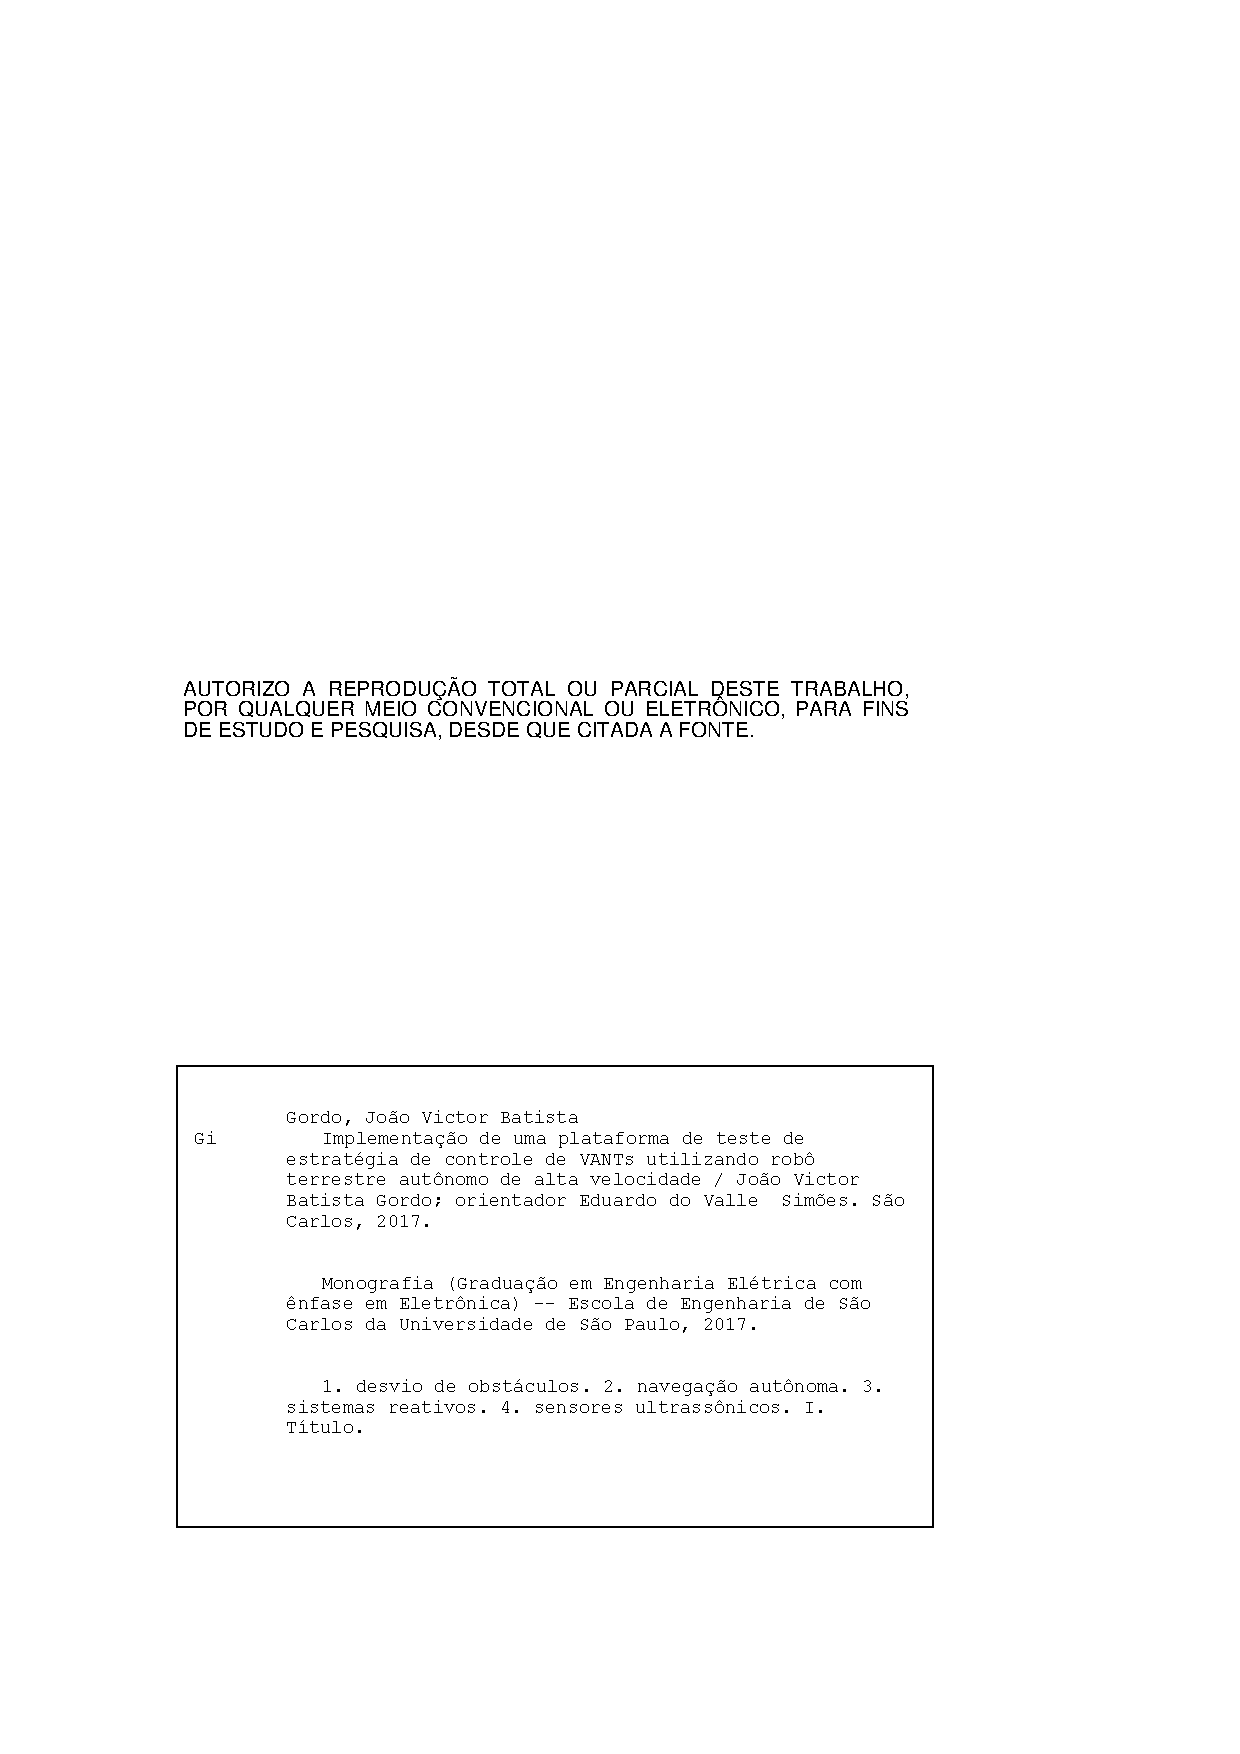
\includepdf{USPSC-Tese-pre-textual/fichacatalografica.pdf} 
% Se você optar por elaborar a ficha catalográfica, deverá 
% incluir uma % antes da linha % antes
% do comando % ---
% Inserir a ficha bibliografica
% ---
% Isto é um exemplo de Ficha Catalográfica, ou ``Dados internacionais de
% catalogação-na-publicação''. Você pode utilizar este modelo como referência. 
% Porém, provavelmente a biblioteca da sua universidade lhe fornecerá um PDF
% com a ficha catalográfica definitiva após a defesa do trabalho. Quando estiver
% com o documento, salve-o como PDF no diretório do seu projeto e substitua todo
% o conteúdo de implementação deste arquivo pelo comando abaixo:
%
\begin{fichacatalografica}
	\hspace{-1.4cm}
	\imprimirnotaautorizacao \\ \\
	%\sffamily
	\vspace*{\fill}					% Posição vertical
	\begin{center}					% Minipage Centralizado
		\imprimirnotabib \\
\begin{table}[htb]
	\scriptsize
	\centering	
	\begin{tabular}{|p{0.9cm} p{8.7cm}|}
		\hline
	      & \\
		  &	  \imprimirautorficha     \\
		
		 \imprimircutter & 
							\hspace{0.4cm}\imprimirtitulo~  / ~\imprimirautor~ ;  ~\imprimirorientadorcorpoficha. -- 	\imprimirlocal, \imprimirdata.   \\
		
		  &  % Para incluir nota referente à versão corrigida no corpo da ficha,
			  % incluir % no início da linha acima e tirar a % do início da linha abaixo
			  %	\hspace{0.4cm} \imprimirtitulo~  / ~\imprimirautor~ ; ~\imprimirorientadorcorpoficha~- ~\imprimirnotafolharosto. -- \imprimirlocal, \imprimirdata.  \\
		
			\hspace{0.4cm}\pageref{LastPage} p. : il. (algumas color.) ; 30 cm.\\ 
		  & \\
		  & 
		    \hspace{0.4cm}\imprimirnotaficha ~--~ 
						  \imprimirunidademin, 
						  \imprimiruniversidademin, 
		                  \imprimirdata. \\ 
		  & \\                 
		   % Para incluir nota referente à versão corrigida em notas,
		    % incluir uma % no início da linha acima e	
		    % tirar a % do início da linha abaixo
		    % & \hspace{0.4cm}\imprimirnotafolharosto \\ 
		  & \\ 
		  & \hspace{0.4cm}1. LaTeX. 2. abnTeX. 3. Classe USPSC. 4. Editoração de texto. 5. Normalização da documentação. 6. Tese. 7. Dissertação. 8. Documentos (elaboração). 9. Documentos eletrônicos. I. \imprimirorientadorficha. 
		   II. Título. \\
	
		     %Se houver co-orientador, inclua % antes da linha (antes de II. Título.) 
		     %          e tire a % antes do comando abaixo 
		     %III. Título. \\   
		  \hline
	\end{tabular}
\end{table}
	\end{center}
\end{fichacatalografica}
% ---

 
% e retirar o % do comando abaixo
%% ---
% Inserir a ficha bibliografica
% ---
% Isto é um exemplo de Ficha Catalográfica, ou ``Dados internacionais de
% catalogação-na-publicação''. Você pode utilizar este modelo como referência. 
% Porém, provavelmente a biblioteca da sua universidade lhe fornecerá um PDF
% com a ficha catalográfica definitiva após a defesa do trabalho. Quando estiver
% com o documento, salve-o como PDF no diretório do seu projeto e substitua todo
% o conteúdo de implementação deste arquivo pelo comando abaixo:
%
\begin{fichacatalografica}
	\hspace{-1.4cm}
	\imprimirnotaautorizacao \\ \\
	%\sffamily
	\vspace*{\fill}					% Posição vertical
	\begin{center}					% Minipage Centralizado
		\imprimirnotabib \\
\begin{table}[htb]
	\scriptsize
	\centering	
	\begin{tabular}{|p{0.9cm} p{8.7cm}|}
		\hline
	      & \\
		  &	  \imprimirautorficha     \\
		
		 \imprimircutter & 
							\hspace{0.4cm}\imprimirtitulo~  / ~\imprimirautor~ ;  ~\imprimirorientadorcorpoficha. -- 	\imprimirlocal, \imprimirdata.   \\
		
		  &  % Para incluir nota referente à versão corrigida no corpo da ficha,
			  % incluir % no início da linha acima e tirar a % do início da linha abaixo
			  %	\hspace{0.4cm} \imprimirtitulo~  / ~\imprimirautor~ ; ~\imprimirorientadorcorpoficha~- ~\imprimirnotafolharosto. -- \imprimirlocal, \imprimirdata.  \\
		
			\hspace{0.4cm}\pageref{LastPage} p. : il. (algumas color.) ; 30 cm.\\ 
		  & \\
		  & 
		    \hspace{0.4cm}\imprimirnotaficha ~--~ 
						  \imprimirunidademin, 
						  \imprimiruniversidademin, 
		                  \imprimirdata. \\ 
		  & \\                 
		   % Para incluir nota referente à versão corrigida em notas,
		    % incluir uma % no início da linha acima e	
		    % tirar a % do início da linha abaixo
		    % & \hspace{0.4cm}\imprimirnotafolharosto \\ 
		  & \\ 
		  & \hspace{0.4cm}1. LaTeX. 2. abnTeX. 3. Classe USPSC. 4. Editoração de texto. 5. Normalização da documentação. 6. Tese. 7. Dissertação. 8. Documentos (elaboração). 9. Documentos eletrônicos. I. \imprimirorientadorficha. 
		   II. Título. \\
	
		     %Se houver co-orientador, inclua % antes da linha (antes de II. Título.) 
		     %          e tire a % antes do comando abaixo 
		     %III. Título. \\   
		  \hline
	\end{tabular}
\end{table}
	\end{center}
\end{fichacatalografica}
% ---


% As informações que compõem a ficha catalográfica estão 
% definidos no arquivo USPSC-pre-textual-UUUU.tex
% ---


% ---
% ---
% Inserir errata
% ---

\begin{errata}
	\OnehalfSpacing 			
	A errata é um elemento opcional, que consiste de uma lista de erros da obra, precedidos pelas folhas e linhas onde eles ocorrem e seguidos pelas correções correspondentes. Deve ser inserida logo após a folha de rosto e conter a referência do trabalho para facilitar sua identificação, conforme a ABNT NBR 14724 \cite{nbr14724}.
	
	Modelo de Errata:
		
	\begin{flushleft} 
			\setlength{\absparsep}{0pt} % ajusta o espaçamento da referência	
			\SingleSpacing 
			\imprimirautorabr~ ~\textbf{\imprimirtitulo}.	\imprimirdata. \pageref{LastPage}p. 
			%Substitua p. por f. quando utilizar oneside em \documentclass
			%\pageref{LastPage}f.
			\imprimirtipotrabalho~-~\imprimirinstituicao, \imprimirlocal, \imprimirdata. 
 	\end{flushleft}
\vspace{\onelineskip}
\OnehalfSpacing 
\center
\textbf{ERRATA}
\vspace{\onelineskip}
\OnehalfSpacing 
\begin{table}[htb]
	\center
	\footnotesize
	\begin{tabular}{p{1.4cm} p{1cm} p{3cm} p{3cm} }
		\hline
		\textbf{Folha} & \textbf{Linha}  & \textbf{Onde se lê}  & \textbf{Leia-se}  \\
			\hline
			1 & 10 & auto-conclavo & autoconclavo\\
		\hline
	\end{tabular}
\end{table}


\end{errata}
% ---

% ---
% Inserir folha de aprovação
% ---

% A Folha de aprovação é um elemento obrigatório da NBR 4724/2011 (seção 4.2.1.3). 
% Após a defesa/aprovação do trabalho, gere o arquivo folhadeaprovacao.pdf da página assinada pela banca 
% e iclua o arquivo utilizando o comando abaixo:
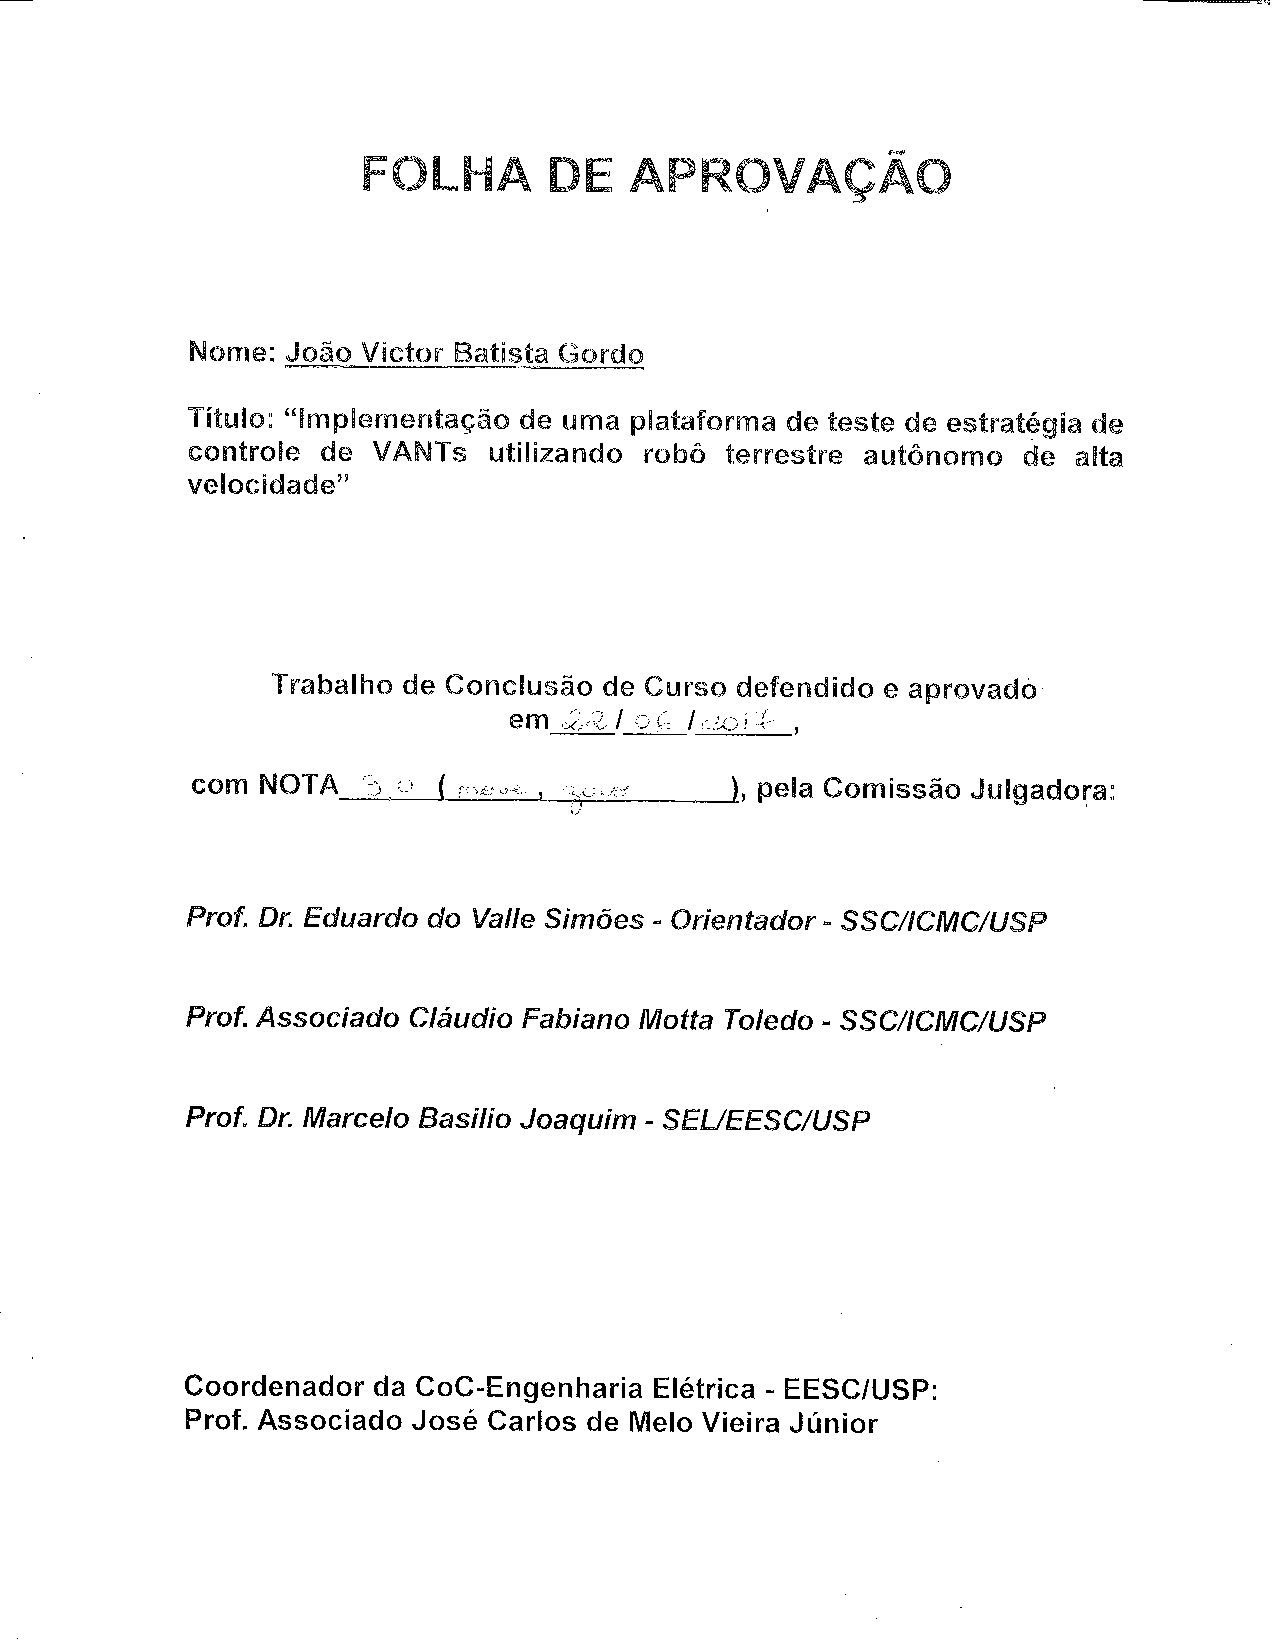
\includepdf{folhadeaprovacao.pdf}
% Alternativa para a Folha de Aprovação:
% Se for a sua opção elaborar uma folha de aprovação, insira uma % antes do comando acima que inclui o arquivo folhadeaprovacao.pdf,
% tire o % do comando abaixo e altere o arquivo folhadeaprovacao.tex conforme suas necessidades
%% Alternativa para a Folha de Aprova��o 
% Se esta for a sua op��o, exclua inclus�o feita acima do arquivo folhadeaprovacao.pdf
%
\begin{folhadeaprovacao}
  \begin{center}
       {\ABNTEXchapterfont\bfseries\large\imprimirautor}
	 \vspace*{2cm}
   
    \begin{center}
      \ABNTEXchapterfont\bfseries\Large\imprimirtitulo
    \end{center}
		\vspace*{2cm}
		\hspace{.45\textwidth}
    \begin{minipage}{.5\textwidth}
        \imprimirpreambulo
    \end{minipage}
		\vspace*{2cm}
    %\vspace*{\fill}
	\end{center}

  \begin{center}
	  {\ABNTEXchapterfont\bfseries\large\ {Trabalho de Conclus\~ao de Curso defendido e aprovado\\
	  em 22 de junho de 2017}, pela Comiss\~ao Julgadora: \\}
		\par
		\vspace*{2cm}
		{\ABNTEXchapterfont\bfseries\large Prof. Dr.  Eduardo do Valle Sim\~oes - Orientador - SSC/ICMC/USP \\}
		\vspace*{1cm}
		{\ABNTEXchapterfont\bfseries\large Prof. Dr.  Marcelo Bas\'ilio Joaquim - SEL/EESC/USP\\}
		\vspace*{1cm}
		{\ABNTEXchapterfont\bfseries\large Prof. Dr.  Cl\'audio Fabiano Motta Toledo - SSC/ICMC/USP \\}
		\vspace*{1cm}
		%\assinatura{\textbf{Professor} \\ Convidado3}
		%\assinatura{\textbf{Professor} \\ Convidado4}
		%\begin{center}
		\vspace*{\fill}
   	{\ABNTEXchapterfont\bfseries\large Coordenador da CoC-Engenharia El\'etrica - EESC/USP: \\}
   	{\ABNTEXchapterfont\bfseries\large Prof. Associado Jos\'e Carlos de Melo Vieira J\'unior}
    \par
\end{center}
\end{folhadeaprovacao}
% ---


\includepdf{PaginaEmBranco.pdf}

% ---
% Dedicatória
% ---
%% USPSC-Dedicatória.tex
% ---
% Dedicatória
% ---
\begin{dedicatoria}
   \vspace*{\fill}
   \centering
   \noindent
   \textit{ Este trabalho é dedicado aos alunos da USP, como uma contribuição\\
  das Bibliotecas do Campus USP de São Carlos para o desenvolvimento\\
	e disseminação da pesquisa científica da Universidade.} \vspace*{\fill}
\end{dedicatoria}
% ---
% ---

% ---
% Agradecimentos
% ---
%% Agradecimentos.tex
% ---
% Agradecimentos
% ---=====
\begin{agradecimentos}
	A motivação para o desenvolvimento da classe USPSC e dos modelos de trabalhos acadêmicos foi decorrente de solicitações de usuários das Bibliotecas do Campus USP de São Carlos. A versão 2.0 do Pacote USPSC é composto da \textbf{Classe USPSC}, do \textbf{Modelo para TCC em \LaTeX\ utilizando a classe USPSC} e do \textbf{Modelo para teses e dissertações em \LaTeX\ utilizando a classe USPSC}.
	
	O Modelo para TCC está disponível inicialmente apenas para EESC e será estendido às demais Unidades de Ensino do Campus USP de São Carlos a medida que as mesmas definirem seus padrões.
	
	O Grupo desenvolvedor do Pacote USPSC agradece especialmente ao Luis Olmes, doutorando do Instituto de Ciências Matemáticas e de Computação (ICMC) da Universidade de São Paulo (USP), pelas primeiras orientações sobre o \LaTeX\ . 
	
	Agradecemos ao Lauro César Araujo pelo desenvolvimento da classe  \abnTeX, modelos canônicos e tantas outras contribuições que nos permitiu o desenvolvimento da classe USPSC e seus modelos.
	
	Os nossos agradecimentos aos integrantes do primeiro
	projeto abn\TeX\, Gerald Weber, Miguel Frasson, Leslie H. Watter, Bruno Parente Lima, Flávio de Vasconcellos Corrêa, Otavio Real
	Salvador, Renato Machnievscz, e a todos que contribuíram para que a produção de trabalhos acadêmicos em conformidade com
	as normas ABNT com \LaTeX\ fosse possível.
	
	Agradecemos ao grupo de usuários
	\emph{latex-br}{\url{http://groups.google.com/group/latex-br}}, aos integrantes do grupo
	\emph{\abnTeX}{\url{http://groups.google.com/group/abntex2}  e \url{http://www.abntex.net.br/}}~que contribuem para a evolução do \abnTeX.
\end{agradecimentos}
% ---
% ---

% ---
% Epígrafe
% ---
\begin{epigrafe}
    \vspace*{\fill}
	\begin{flushright}
		\textit{``O estudo, a busca da verdade e da beleza são domínios \\
		em que nos é consentido sermos crianças por toda a vida.''\\
		Albert Einstein}
	\end{flushright}
\end{epigrafe}
% ---

% A T E N Ç Ã O
% Se o idioma do texto for em inglês, o abstract deve preceder o resumo
% resumo em português
%
% Resumo
% ---

% resumo em português
\setlength{\absparsep}{18pt} % ajusta o espaçamento dos parágrafos do resumo
\begin{resumo}
Foi implementado um veículo de navegação autônoma de alta velocidade, cuja técnica de desvio de obstáculos é puramente reativa, com o propósito de 
servir como uma plataforma de testes de navegação de VANTs desenvolvidos na arquitetura MOSA, que desacopla a porção crítica da não crítica do 
sistema embarcado de tempo real.
A percepção do veículo consiste em uma matriz de cinco sensores ultrassônicos, o subsistema de locomoção funciona por tração dianteira feita por 
motores de corrente contínua sem escovas, o subsistema de comunicação é feito via rádio com as funcionalidades de: obtenção remota de dados 
internos do veículo durante a navegação autônoma, de uma interface de comando que também possibilitasse a mudança de variáveis internas do veículo sem 
a necessidade de reprogramar o microcontrolador e, o mais importante, de dar ou não ao veículo o aval para navegar com base no \textit{status} de um 
botão de segurança acoplado a outro rádio.
A estratégia de navegação consiste em classificar as leituras de cada um dos sonares em três regiões: distante, atenção e próxima; com base em qual 
região encontra-se cada sonar, toma-se a decisão de qual a medida de evasão a ser realizada, isto é, foi gravada na memória do microcontrolador uma 
tabela que correlaciona cada uma das combinações de regiões a um par ordenado de velocidades que deve ser imposta aos motores para desviar do 
obstáculo em questão.
Contudo, as leituras obtidas pelos sonares foram fortemente afetadas em decorrência de vibrações mecânicas dos motores, que causam leituras 
espúrias, o que, por sua vez, provoca a adoção de comportamentos errados pelo veículo.

 \textbf{Palavras-chaves}: navegação autônoma. sistemas reativos. sensores ultrassônicos. desvio de obstáculos.
\end{resumo}

% ---

% Abstract
% ---
%% Abstract.tex
% ---
% Abstract
% ---
\autor{Gordo, J.V.B.}
 \begin{resumo}[Abstract]
  \begin{otherlanguage*}{english}
 A high speed autonomous mobile robot with a purely reactive obstacle avoidance technique was implemented. Its purpose is to serve as a navigation 
test platform for UVAs in MOSA architecture which decouples the critical from the non-critical portion in the embedded system at real time. The 
vehicle’s perception is composed of an array of five ultrasonic sensors, the locomotion subsystem operates by front-wheel drive made through brushless 
DC motors, the communication subsystem is made through radio and its functions are: obtaining remote internal data during the autonomous navigation as 
well as a command interface which could also enable changes on the internal variables of the vehicle without reprograming the microcontroller and, 
most important, endorse the vehicle’s navigation based on the status of a security button attached to another radio. The navigation strategy consists 
in classifying the readings from each of the sonars in three regions: distant, warning and close. Based on the region where the sonar is located, a 
decision is made on which evasion measure is to be carried out, i.e., in the microcontroller’s memory was recorded a table that correlates each 
combinations of regions to an ordered pair of speed which has to be imposed to the motors so they are able to deviate from the obstacle. However, the 
readings obtained by the sonars were strongly affected by the mechanical vibrations from the motors, causing spurious readings which led the vehicle 
to adopt wrong behaviors.

    \vspace{\onelineskip}
  
    \noindent 
    \textbf{Key-words}: autonomous navigation. reactive systems. ultrasonic sensors. obstacle avoidance
  \end{otherlanguage*}
 \end{resumo}

% ---

% ---
% inserir lista de figurass
% ---
\pdfbookmark[0]{\listfigurename}{lof}
\listoffigures*
\cleardoublepage
% ---

% ---
% inserir lista de tabelas
% ---
\pdfbookmark[0]{\listtablename}{lot}
\listoftables*
\cleardoublepage
% ---

% ---
% inserir lista de quadros
% ---
\pdfbookmark[0]{\listofquadroname}{loq}
\listofquadro*
\cleardoublepage
% ---

% ---
% inserir lista de abreviaturas e siglas
% ---
\begin{siglas}
    \item[ABNT] Associação Brasileira de Normas Técnicas
    \item[abnTeX] ABsurdas Normas para TeX
	\item[EESC] Escola de Engenharia de São Carlos
	\item[IAU] Instituto de Arquitetura e Urbanismo
	\item[IBGE] Instituto Brasileiro de Geografia e Estatística
	\item[ICMC] Instituto de Ciências Matemáticas e de Computação
	\item[IFSC] Instituto de Física de São Carlos
	\item[IQSC] Instituto de Química de São Carlos
	\item[PDF] Portable Document Format
	\item[TCC] Trabalho de Conclusão de Curso
	\item[USP] Universidade de São Paulo
	\item[USPSC] Campus USP de São Carlos
	
\end{siglas}
% ---

% ---
% inserir lista de símbolos
% ---
\begin{simbolos}
  \item[$ \Gamma $] Letra grega Gama
  \item[$ \Lambda $] Lambda
  \item[$ \zeta $] Letra grega minúscula zeta
  \item[$ \in $] Pertence
\end{simbolos}
% ---
% ---
% inserir o sumario
% ---
\pdfbookmark[0]{\contentsname}{toc}
\tableofcontents*
\cleardoublepage
% ---
% ----------------------------------------------------------
% ELEMENTOS TEXTUAIS
% ----------------------------------------------------------
\textual
% Os capítulos são inseridos como arquivos externos 

% Capítulo 1 - Introdução
% ---
%% USPSC-Introducao.tex

% ----------------------------------------------------------
% Introdução (exemplo de capítulo sem numeração, mas presente no Sumário)
% ----------------------------------------------------------
\chapter[Introdução]{Introdução}

O presente trabalho consiste na implementação de um veículo autônomo de alta
velocidade, desenvolvido sob o paradigma de sistemas puramente reativos, cuja finalidade
é servir como uma plataforma terrestre de testes de estratégias de navegação de Veículos
Aereos Não Tripulados, VANTs, dentro da arquitetura MOSA, \textit{Mission Oriented Sensor
Array}. Isto é, na arquitetura MOSA, o escopo deste projeto consiste na porção relativa
à aeronave, que é responsável por cuidar da integridade do veículo, enquanto a parte
orientada à missão é o que pretende-se testar utilizando o veículo. A necessidade de
se desenvolver um veículo terrestre para testar \textit{drones} se dá pelo fato de que o este é
um sistema embarcado crítico cuja falha pode resultar em acidentes graves, logo, caso o
comportamento do MOSA desenvolvido seja extensivamente testado em um ambiente livre
de riscos utilizando-se o veículo, há menos risco de eventuais danos provocados por mal
funcionamento. Maiores detalhes acerca da arquitetura MOSA serão abordados na seção
de Embasamento Teórico.

O projeto pode ser dividido em 4 subsistemas: percepção, locomoção, comunicação
e navegação. A percepção é feita através de uma matriz de cinco sensores ultrassônicos
de baixo custo, que são disparados simultaneamente a fim de reduzir o tempo gasto
com obtenção dos dados do ambiente externo. Como consequência disso, obtém-se dados
menos confiáveis pois são intensificados efeitos colaterais como o crosstalk, que não pode ser
eliminado processando medidas consecutivas, conforme \cite{2016_artigo_1}. Além disso, buscou-se verificar
o quão significativo é o impacto na confiabilidade das medidas caso os ciclos de leitura dos
sonares seja determinado de acordo com as circunstâncias do meio, isto é, caso não haja
um intervalo de medição fixo e pré-determinado, denominado intervalo estático de agora
em diante, de modo que o período gasto na percepção estivesse atrelado apenas ao tempo
gasto pelo sonar que detectou o obstáculo mais distante do veículo, denominado intervalo
dinâmico. Ao adotar intervalos dinâmicos, reduz-se o tempo entre leituras consecutivas,
o que pode fazer com que vibrações residuais da membrana responsável por emitir as
ondas acústicas sensibilize o elemento receptor provocando falsas leituras, conforme \cite{jones}.
Maiores detalhes acerca do princípio de funcionamento dos sensores ultrassônicos, assim
como vantagens e desvantagens deste sensor encontram-se na seção de Materiais desta
monografia.

Para a locomoção do veículo, são utilizados dois motores \textit{brushless} de corrente
contínua, de modo que a tração é dianteira. Logo, o veículo faz curvas em razão da diferença
de velocidade entre os BLDC e, por se tratar de motores usualmente utilizados em VANTs,
atinge velocidade de até  \unitfrac[80]{km}{h}.
Como o controle de motores sem escovas não é trivial de
ser feito, foram utilizados controladores eletrônicos de velocidade, ESCs, como elemento
intermediador entre o microcontrolador e os motores. Desta forma, todo o tratamento de
mais baixo nível no que concerne o acionamento das bobinas dos motores foi designado
a este dispositivo, enquanto o microcontrolador se responsabiliza por fornecer aos ESCs
a velocidade que pretende-se obter do seu respectivo motor.
O sistema de comunicação tem o propósito de: fornecer feedback dos dados internos
do veículo, como percepção e velocidade dos motores; regular o acionamento dos motores,
pois repassa ao microcontrolador informações de um botão de segurança, que emite sinais
ao veículo, autorizando-o ou não a navegar; e, finalmente, de servir como uma interface de
comandos na qual é possível controlar remotamente o veículo.
\footnote{Entenda-se por veículo não só a parte física como rodas, motores e dispositivos mas, também, todo o \textit{software} responsável por gerir 
o automóvel.}.

Quanto ao subsistema de navegação, temos que este consiste na inteligência artificial
do veículo, isto é, qual é a estratégia utilizada para efetuar o desvio de obstáculos com
base nos dados colhidos pelos sonares. A técnica de desvio de obstáculos implementada
é a mais simples possível: trata-se de uma função que mapeia as leituras dos sonares -
categorizadas em três regiões: perigo, atenção e distante - em um par de velocidades
angulares - categorizados quanto a intensidade em forte, médio e leve, e quanto à direção
em esquerda ou direita - a serem impostas aos motores de acordo com qual a combinação
de regiões lida pela matriz de sonares, conforme a Eq. \ref{nav}. A tabela verdade que relaciona
domínio e contradomínio da função de desvio de obstáculos consta no Apêndice, vide Tabela \ref{IA}.

\begin{equation}
\label{nav}
T:R^5 \rightarrow S \\
\end{equation}
$$\quad \textrm{em que:} \quad R=\{distante, perigo, atenção\}, \quad S=\{E_L, E_M, E_F, D_L, D_M, D_F\}$$

Note que cada um dos elementos do conjunto S são pares ordenados que representam a
velocidade angular dos motores.

A título de ilustração, para deixar mais claro o propósito deste projeto, podemos
supor que um MOSA esteja sendo desenvolvido com o propósito de percorrer uma rota
previamente selecionada, utilizando-se de GPS, acelerômetro e magnetômetro para a
missão. Este poderia ser testado no veículo antes de ser colocado para voar, de forma que
o veículo autônomo desempenharia a função da aeronave, sendo responsável por desviar
de eventuais obstáculos quando necessário, e quando o caminho estiver livre, o controle
do veículo seria repassado ao MOSA, mas ainda sob sua supervisão. Dessa forma, quando
em posse do veículo, o MOSA desempenharia sua missão, que no exemplo citado seria
percorrer \textit{checkpoints}.

% ---

% ---
% Capítulo 2
% ---
\chapter[Embasamento Teórico]{Embasamento Teórico}
\section{Sistemas Reativos}
\epigraph{ 
	  \textit{``Representações explícitas e modelos atrapalham. No fim das contas, a melhor representação do mundo é ele mesmo.''} 
	 }
	  { Brooks, R.A \cite{brooks} - tradução livre -} 
	  
%   \begin{flushright}
% 	  \textit{``Representações explícitas e modelos atrapalham.\\
% 	  No fim das contas, a melhor representação \\
% 	  do mundo é ele mesmo.", Brooks, R.A. 
% 	  \cite{brooks} \footnote{tradução livre}}
%   \end{flushright}

\subsection{Paradigma Reativo como Robótica Bioinspirada} 

De acordo com Rodney Brooks \cite{brooks}, para o desenvolvimento da inteligência no seu sentido mais estrito e genuíno, são condições 
suficientes que o indivíduo, que denominaremos agente, tenha as seguintes faculdades: mobilidade dentro de um ambiente dinâmico no qual esteja 
inserido, percepção do que se passa nas suas adjacências e, por fim, manutenção da própria sobrevivência.
Em suma, habilidades como o raciocinar, comunicar-se e gerar conhecimento nada mais são do que comportamentos complexos, consequências simples do 
fato 
de existirmos e do nosso poder de reação dentro do meio em que vivemos.

Para aprofundarmos a discussão e esclarecermos como se daria esse processo de aprimoramento dos agentes, é preciso fornecer uma  definição 
mais rigorosa do termo ``comportamento''.
Em tradução livre: ``comportamentos são mapeamentos diretos de informações sensoriais recebidas em  
padrões de ações motoras, desempenhadas para se cumprir uma tarefa. Matematicamente, seria uma função transferência que transforma dados dos 
sensores em comandos para os atuadores'' \cite{murphy}.

Nos animais, a transformação de percepção em ação está subordinada à existência de estímulos específicos de natureza interna ou externa 
ao agente que podem ser entendidos como sinais de controle, permitindo ou inibindo determinados comportamentos \cite{murphy}.
A título de ilustração: ao avistar uma presa - informação sensorial - o predador somente a ataca - comportamento - caso esteja com fome - estímulo 
interno; ou quando afastamos a mão - comportamento - ao tocarmos uma panela quente - a informação sensorial seria a temperatura da panela enquanto o 
estímulo externo é o fato de que ela excede uma dada temperatura.

Com base em estudos da etologia, os comportamentos dos animais podem ser inatos ou aprendidos, e a sua inteligência pode ser decomposta verticalmente 
em camadas de comportamentos, cada qual acessa os sensores e atuadores do agente de maneira independente das demais \cite{murphy}.
Isto é, o indivíduo inicia sua existência com um conjunto de comportamentos inatos de autopreservação mas, ao longo da sua vida, outros 
novos vão surgindo, podendo: refinar comportamentos pré-existentes, negá-los (completamente) ou agregar a eles sem produzir conflitos, 
i.e. trabalhando paralelamente com os que lhe são ancestrais.
Desta forma, os dois primeiros casos podem ser entendidos como uma reutilização de camadas inferiores da inteligência, enquanto o 
último consiste na adição de mais uma camada.

\subsection{Características}
Por estar embasado em ideias da etologia discutidas na seção anterior, o paradigma reativo simplesmente desconsidera a etapa de planejamento 
existente na tríade 'percepção, planejamento, ação', que sumariza o ciclo de tarefas realizadas por um sistema sob o paradigma hierárquico 
\cite{murphy,roseli}.
Em suma, os comportamentos se dão de acordo com o que o agente percebe que está acontecendo no seu entorno, não são feitas modelagens ou 
representações do ambiente externo, apenas medições locais e orientadas a comportamentos.

Em decorrência da exclusão da etapa de planejamento, robôs desenvolvidos sob o paradigma reativo costumam ser simples e apresentam 
respostas rápidas \cite{roseli}.
Com boas práticas de projeto é possível construir um robô com: alta coesão, pois comportamentos podem ter acesso direto aos sensores de que 
necessitam para tomar suas decisões - o que possibilita um alto grau de independência em relação a operações e dados externos entre diferentes 
módulos 
ou subsistemas do robô; e baixo acoplamento, pois comportamentos são independentes entre si e, portanto, há pouca ou nenhuma dependência de ligações 
e 
interfaces externas a um dado módulo \cite{murphy}.

% TODO: \subsection{Arquitetura de Subsumpção}

\section{Arquitetura MOSA}

Arquitetura que propõe dividir o sistema aéreos de navegação autônoma em dois módulos: aeronave e MOSA \cite{mosa_proposal}.

O primeiro constitui a porção crítica do sistema embarcado, i.e. segmento cuja falha pode resultar em ao menos um dos seguintes desastres: morte 
ou lesão de pessoas; destruição ou danos a propriedades, patrimônios ou equipamentos; danos ambientais \cite{safety}.
Veículos Aéreos Não Tripulados, VANTs, apresentam a tolerância de um erro grave a cada $10^5$ ou $10^9$ horas de voo \cite{hard}, o que os 
caracteriza
como sistemas computacionais de tempo real do tipo \textit{hard}. 
Maiores esclarecimentos acerca destes jargões podem ser encontrados no apêndice.

O segundo corresponde à parte não crítica à segurança, encarregada do controle da navegação e, por conseguinte, da determinação da maior parte dos 
parâmetros de voo. É caracterizado como um conjunto de sensores inteligentes capazes de cumprir uma missão específica, ou seja, 
existe uma relação biunívoca entre missão e MOSA, dado que ele consiste no melhor arranjo de sensores para o cenário em questão. Neste contexto, a 
aeronave é vista unicamente como o meio de transporte dos sensores, enquanto que o módulo MOSA constituiria o \textquoteleft cérebro\textquoteright{}  
da plataforma, responsável pelo cumprimento da missão e por guiar a aeronave até a sua realização.

%  \begin{figure}[h]
%   \includegraphics[scale=0.5]{./Resources/MOSA.png}
%   \caption{MOSA} \label{MOSA}
%  \end{figure}

No entanto, como a aeronave é o elemento responsável pela garantia da segurança, cabe a ela acatar ou não os comandos do MOSA. E pode, inclusive, 
optar por readaptar a missão em tempo de voo para se ajustar ao cenário, o que inclui a seleção dos sensores que melhor se encaixam na dada 
conjuntura.

Isso se dá através de uma matriz de reconfiguração dinamicamente adaptável denominada \textit{Knowledge Based Framework}, seu papel é comparável à 
expertise de um piloto.
Ou seja, um elemento inteligente capaz de escolher o melhor serviço  a ser executado com base em regras e critérios de seleção, tais quais resposta 
em tempo 
real, segurança e performance.


% diferentes missões, definidas pelo mosa e diferentes sensores, podem ser integrados, possibilitando a escolha do melhor arranjo de sensores que se 
% ajuste ao cenário de utilização do sistema. este é o mecanismo básico do mosa, fazendo com que a missão possa ser adaptativa. durante uma missão, 
% com 
% base em uma matriz de reconfiguração o vant pode se adaptar dinamicamente às características da missão, escolhendo os sensores que melhor se 
% encaixam 
% dependendo da situação. além do hardware, um sistema mosa deve contemplar também o software capaz de realizar uma missão, comunicar-se com todos os 
% sensores que o compõe, enviar e receber dados para a aeronave .
% 
% o sistema mosa deve ser capaz de determinar se a missão prevista pode ou não ser realizada.
% 
% the aircraft can, for safety reasons, not follow the flight sensors
% commands, eventually terminating the flight
% 
% flight sensors can provide data for mission controllers but aircraft
% % % % % % % % controllers must not use data provided by mission sensors


\chapter{Materiais}
\begin{itemize} %% TODO: colocar as rodas: http://www.hobbyking.com/hobbyking/store/__2176__598__Hardware_Accessories-Wheels_0_40mm.html
 \item 5 sensores ultrassônicos de distância HC-SR04
 \item 2 motores \textit{brushless outrunner} Turnigy D2836/9 950KV
 \item 2 ESCs Hobby King com UBEC de 5.5V/4A: um de 35A e outro de 40A 
 \item 2 módulos de rádio frequência baseados no \textit{transceiver} Nordic nRF24L01+ 
 \item 1 bateria LiPo 30C de 2800 mAh
 \item 2 Arduino Pro Mini
 \item 1 Conversor/Adaptador USB-Serial PL2303
 \item 1 Carregador balanceador de bateria IMAX B6-AC
\end{itemize}

\section{Motor \textit{Brushless}}
São motores síncronos\footnote{Motores Síncronos: o campo magnético girante do rotor e do estator têm a mesma frequência.} de corrente contínua cuja 
comutação é feita eletronicamente, e não mecanicamente por meio de escovas como nos motores CC comuns, por isso denominados \textit{brushless}.
Possui aplicações nas indústrias de automóveis, aeroespacial, médica, de equipamentos de automação industrial e instrumentação .
Os motores BLDC apresentam algumas vantagens em relação aos de corrente contínua com escovas e de indução no que concerne a: resposta 
dinâmica, ruídos 
de operação, durabilidade (i.e. vida útil), assim como razão do torque pelas dimensões do motor \cite{motor_2}. 

% TODO tava uma merda, reler pois alterei um pouco
O rotor consiste de um imã permanente, já os pólos do estator são formados por enrolamentos, que precisam ser energizados na sequência correta 
para que um campo magnético girante seja criado.
Nas máquinas CC isto é feito mecanicamente através das escovas mas, no caso do BLDC, é preciso que a posição do rotor em relação ao estator seja 
conhecida para que seja possível fazer o acionamento correta das bobinas.
Existem dois meios de se obter esta informação: através de sensores de efeito hall, método empregado neste trabalho, ou processamento da força contra 
eletromotriz das bobinas do estator.

Sensores de efeito Hall são transdutores analógicos que relacionam a intensidade do campo magnético externo transversalmente disposto a ele em termos 
de tensão elétrica. Quando associado a um circuito comparador \textit{schmitt trigger}, comportam-se como um sensor digital que aponta quando a 
intensidade do campo magnético atinge um valor de limiar pré-determinado. Ao dispor sensores deste tipo ao longo do estator, torna-se possível uma 
estimativa da posição do rotor ao ser feito um estudo comparativo da resposta de cada sensor, cruzando esta informação com a posição que 
cada um destes se encontra em relação ao estator \cite{motor_1}.

Há a possibilidade de fazer a comutação sem empregar qualquer tipo de sensor, logo, trata-se de um método mais barato. 
Nesse caso, a estimativa da posição do rotor se dá através do processamento das forças contra-eletromotriz de cada um dos enrolamentos do estator.
No entanto, algumas limitações surgem: o motor deve operar acima de uma dada rotação, caso contrário o método não funciona; mudanças bruscas de carga 
não podem ocorrer; há discontinuidades na resposta do motor quando operando em velocidades acima da taxa de comutação ideal \cite{motor_1}.

\section{ESC}
Controlador responsável por processar as informações oriundas dos sensores de efeito Hall do motor BLDC e providenciar o acionamento correto 
dos enrolamentos do estator para que a velocidade angular se dê de acordo com o sinal de controle que é enviado a este dispositivo.
No caso dos ESCs utilizados no presente trabalho, este sinal de controle é feito utilizando-se modulação por largura de pulso, i.e. PWM. 
A frequência de operação varia de acordo com o modelo do controlador e para o caso deste projeto é de 400Hz.
%% TODO: \cite{carlson}
%% TODO: fazer uma descrição mais rica de como funciona este dispositivo.
%% TODO: citar que toda a programação do ESC é feita via pwm.
\section{Sensor Ultrassônico}

\subsection{Princípio de Funcionamento}
Utiliza o método \textit{time of flight}, que consiste na medição do intervalo de tempo, igualmente denominado \textit{time of flight}, que uma onda 
ou partícula leva para percorrer uma determinada distância em um dado meio. 
Pode ser utilizado para medir: distância, velocidade \cite{TOF_velocity}e propriedades do meio de propagação ou da partícula propagante
\cite{TOF_medium1,TOF_medium2}.

Para medidores de proximidade, como é o caso de sonares e lasers, um transdutor emissor faz a conversão do sinal elétrico, denominado 
\textit{trigger}, em um pulso de ondas (acústicas para o caso do sonar e eletromagnéticas para o laser), dando início à medição de tempo.
Quando esta onda propagante encontra um objeto que a reflita de volta ao sensor e a intensidade deste sinal recebido, denominado \textit{echo}, está 
acima de um determinado valor de limiar, o transdutor receptor envia um sinal elétrico que interrompe a contagem de tempo, obtendo-se 
assim a medida do \textit{time of flight}, $\tau$.
Com isso, supondo que a velocidade de propagação, $\nu$, desta onda no meio seja conhecida. De acordo com \cite{siegwart}, pode-se 
calcular a distância, $\Delta$, entre o sensor e o objeto que reflete o pulso de ondas pela equação \ref{TOF_eq}:
\begin{equation}
 \label{TOF_eq}
 \Delta = \frac{\nu \times \tau }{2}
\end{equation}

Quanto ao sensor ultrassonico especificamente, temos que as ondas sonoras utilizadas estão usualmente situadas entre 40kHz e 180kHz, sendo 
emitidas no formato de pacotes compostos por uma série de pulsos; no caso do sonar utilizado neste trabalho, 8 pulsos de 40kHz. 
Por se tratarem de ondas mecânicas, é importante que a tensão de limiar, do inglês \textit{threshold}, comporte-se ao longo do ciclo de 
leitura da seguinte forma \cite{siegwart}: 
durante o período denominado \textit{blanking time}\cite{siegwart}  ou \textit{dead time}\cite{murphy}, o qual engloba o intervalo de 
emissão das ondas sonoras até o momento em que o diafragma para de oscilar (o que pode constituir alguns milisegundos após a cessação do sinal de 
\textit{trigger}), a tensão de limiar é muito alta no intuito de eliminar leituras inválidas decorrentes de interferência entre emissor e receptor; em 
seguida, a tensão de \textit{threshold} se reduz a um valor que permita a detecção de obstáculos e vai sendo continuamente decrementada com o passar 
do tempo. 
Isso se dá pelo fato de que a intensidade do sinal acústico, i.e. potência por ângulo sólido, sofre atenuações atmosféricas que variam com a 
distância percorrida, conforme a equação \ref{Atm_Attenuation} \cite{everett}, que leva em consideração somente efeitos da divergência esférica e 
absorção molecular.
\begin{equation}
 \label{Atm_Attenuation}
 I = \frac{ I_0 e^{-2 \alpha R} }{4 \pi R^2}
\end{equation}
Em que: $\alpha$ é o coeficiente de atenuação do meio, associado às absorções moleculares, o qual varia em função da frequência da onda emitida 
assim como de propriedades do meio, e.g. umidade e poeira contida no ar.
Para ondas de 40kHz: $\unitfrac[0,197]{dB}{m} < \alpha <  \unitfrac[0,295]{dB}{m}$. % TODO posso deixar essa desigualdade aqui???

\subsection{Limitações}

\subsubsection{Variação na velocidade de propagação da onda acústica}
Como citado anteriormente, a medição da distância pressupõe que a velocidade de propagação da onda no meio é conhecida. 
No entanto, mudanças na temperatura e umidade do fluido em que a onda se propaga podem causar erros de medida não desprezíveis \cite{everett}.

\subsubsection{Direcionalidade}
O emissor da radiação acústica ultrassônica apresenta um padrão de radiação\cite{balanis,pozar} composto por lobos laterais\cite{balanis,pozar} que 
não são levados em conta, pois a maioria dos sistemas supõem toda radiação recebida como oriunda do lobo central\cite{balanis,pozar}, usualmente 
modelado como um cone de aproximadamente $30^o$ que varre até 5 metros \cite{murphy}. De acordo com \cite{HC-SR04}, para o dispositivo utilizado 
nesse trabalho o ângulo de abertura do feixe é de $15^o$ e o alcance, 4 metros.

Além deste problema, o próprio fato de que a direcionalidade do sensor é baixa, i.e. o lobo central é largo, implica numa 
imprecisão na medida obtida, pois não é possível associar a distância lida a um lugar específico, mas sim a uma região no espaço coberta pelo lobo 
central \cite{siegwart}.

\subsubsection{Resposta no Ambiente Alvo}
Por ser um sensor refletivo, a performance do sonar é significativamente afetada pelas características do alvo \cite{everett}.
Um dos problemas decorrentes desse fato é que determinados objetos apresentam elevada taxa de absorção ou, ao contrário, são atravessados pela 
radiação, resultando, em ambos os casos, em pouca ou nenhuma energia retornando ao sensor. Dessa forma, estes objetos são invisíveis para o dado 
método de medição; materiais como espuma, pele e roupas podem absorver as ondas acústicas \cite{siegwart} enquanto objetos com áreas superficiais 
pequenas, e.g. mesas e cadeiras, podem não ser detectados \cite{murphy}. Vale ressaltar que as propriedades de reflexão, absorção e transmissão 
são variáveis de acordo com a frequência e com o tipo de radiação, esta podendo ser acústica ou eletromagnética.
%% TODO achar alguém que falou isso e explica absorção reflexão e transmissão
Existem outros problemas relativos ao ambiente alvo que não são relacionados à absorção ou transmissão da radiação, mas sim à reflexão e que serão 
tratados nas 
seções subsequentes separadamente.

\subsubsection{\textit{Foreshortening}}
Como a direcionalidade dos sensores ultrassônicos é baixa, isto é a largura de feixe do lobo central é alta, aproximadamente $30^o$, quando o alvo 
a ser detectado não está perpendicularmente posicionado em relação ao eixo acústico do sensor, o cone que formado pelo lobo principal atinge o objeto 
em instantes diferentes. Consequentemente, retorna ao sensor em instantes diferentes provocando um desvio na leitura da distância, fazendo com que o 
obstáculo pareça estar mais próximo do que está na realidade. Por isso este problema é denominado \textit{foreshortening}

\subsubsection{Reflexão especular e \textit{Crosstalk}}
Analisando ainda a situação em que o obstáculo não está perpendicular ao eixo acústico do sonar, a onda emitida pode ser refletida de tal 
forma que não retorne ao sensor, caso este em que o obstáculo não é percebido; outra possibilidade é de que esta onda atinja outras superfícies até 
que por fim retorne ao sensor, desta forma a medida obtida indica que o alvo encontra-se mais distante do que realmente está, fenômeno denominado 
reflexão especular \cite{roseli,siegwart,everett}.  

Quando utiliza-se uma matriz de sonares, este problema é agravado, pois pode provocar interferência entre sensores ou, do inglês, \textit{crosstalk}.
De modo que além da medida obtida estar errada, o posicionamento estimado do obstáculo será também errôneo \cite{murphy}, afinal pressupõe-se que o 
sinal de \textit{echo} é oriundo do pulso de ondas emitido pelo próprio dispositivo.
No entanto, diferentemente da reflexão especular, este problema pode ser amenizado de diferentes maneiras, vide \cite{2016_artigo_1,2016_artigo_5}.

\subsubsection{Tempo de Resposta} %% TODO:


\section{Módulo de rádio frequência}

  \begin{figure}[!htb] %% TODO ver a fonte dessa figura
    \centering
    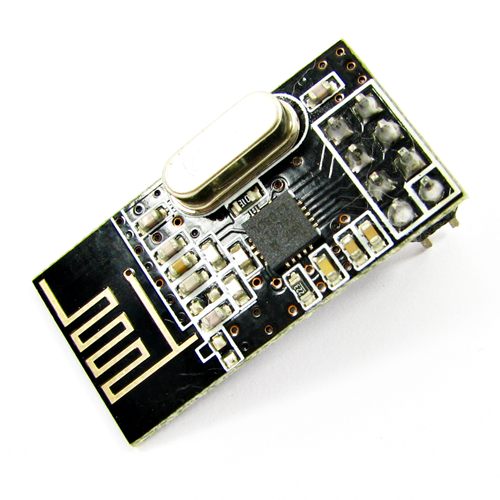
\includegraphics[width=0.5\linewidth]{../../Imagens/nordicc.png}
    \caption{Módulo de Rádio Frequência baseado no \textit{transceiver} da Nordic nRF24L01+}
    \label{Nordic}
  \end{figure}
Módulo de rádio frequência ( Fig. \ref{Nordic}) de baixo custo e consumo cuja faixa de operação situa-se na banda S das ondas UHF ( \textit{Ultra 
High Frequency} ), com uma porção dentro da banda ISM \footnote{maiores informações no apêndice}.
Algumas informações técnicas \cite{nRF} de interesse estão listadas abaixo: 
\begin{itemize}
 \item Tensão de alimentação: 1,9V - 3,6V
 \item Antena em circuito impresso do tipo MIFA(\textit{Meandered Inverted-F Antenna}) \cite{MIFA}
 \item Frequência de operação: 2,4GHz - 2,525GHz
 \item Modulação digital do tipo GFSK 
 \item Apresenta até 126 canais de comunicação \footnote{Válido apenas para as taxas de 250kbps e 1 Mbps; a 2Mbps este valor cai à metade, i.e. 63 
canais.}
 \item Taxas de bits: 250kbps, 1Mbps ou 2Mbps
 \item Potências de saída de transmissão: 0dBm, -6dBm, -12dBm e -18dBm
 \item Interface com o microcontrolador por SPI à taxa de até 10Mbps
 \item Pinos de entrada tolerantes a até 5V
 \item 
Pacotes recebidos verificados automaticamente, certificando-se da validade do endereço apontado e legitimando a integridade 
do pacote via CRC(\textit{Cyclic Redundancy Check}) \footnote{Vide apêndice para uma breve explanação sobre CRC}, antes de 
serem movidos às filas de dados recebidos (\textit{RX FIFO})
 \item Receptor envia ao transmissor um pacote de confirmação de recepção dos dados pelo mesmo canal (\textit{acknowledgment packet}).
\end{itemize}

\section{Arduino}
Trata-se de uma plataforma de prototipação eletrônica aberta, i.e. \textit{open-source hardware}, baseada no microcontrolador de 8 bits da Atmel 
ATMega328 \cite{ATMega}, programável via serial (ICSP) através de um microcomputador, por exemplo, por meio do ambiente de desenvolvimento 
\textit{Arduino Software IDE}, \textit{open-source software} e encontra-se no GitHub \cite{ArduSoft}.
Para programar este dispositivo, foi utilizado um módulo baseado na ponte USB-Serial PL-2303, cuja descrição detalhada pode ser encontrada em 
\cite{PL2303}.

Algumas informações técnicas \cite{ArduInfo} de interesse estão listadas abaixo: 
\begin{itemize}
 \item Dimensões: 17,78mm x 33mm
 \item Tensão de alimentação recomendável: 5V - 12V
 \item Memória 
 \begin{itemize}
  \item Flash: 32kB 
  \item SRAM: 2kB
  \item EEPROM: 1kB
 \end{itemize}

 \item 20 portas digitais de entrada/saída, das quais 6 podem ser usadas como saídas PWM
 \item 6 portas de entrada analógicas
 \item \textit{clock} de 16MHz
\end{itemize}


\section{Bateria} % TODO
Baterias do tipo LiPo são uma das mais indicadas para veículos elétricos e híbridos, tanto quanto para equipamentos eletrônicos portáteis; no 
entanto, alguns cuidados precisam ser tomados ao manipulá-la por serem sensíveis a sobrecarga ou descarga abrupta.
Logo, por questões de segurança e eficiência é necessário haver um sistema eletrônico para gerenciar a recarga deste dispositivo, o qual monitora a 
tensão de cada uma das células assim como a temperatura em pontos específicos \cite{battery}.
Neste trabalho foi utilizado o carregador IMAX B6-AC para fazer este serviço.
\subsection{\textit{C rate}}
É um parâmetro que descreve a corrente de descarga da bateria em relação à sua capacidade nominal \cite{bateria}.
Vide a Eq. \ref{C rate} para um exemplo ilustrativo baseado na bateria utilizada neste projeto.

\begin{equation}
 \label{C rate}
 30 C = \frac{ I_{descarga} }{ 2.800 mAh} \Rightarrow I_{descarga} \approx 10.7A
\end{equation}



\chapter{Método}
\section{Estratégia \textit{bottom-up}}
A estratégia gerencial e organizacional \textit{bottom-up} foi utilizada no desenvolvimento deste projeto. 
Em função da natureza modular e orientada a comportamentos de arquiteturas reativas \cite{murphy}, a adoção deste método de gerenciamento é quase que 
uma escolha natural.
O robô foi dividido em quatro subsistemas, desenvolvidos e testados separadamente: percepção, locomoção, comunicação e navegação (que, no caso deste 
projeto, consiste no desvio de obstáculos em si). %% TODO citar a arq MOSA aqui pra falar do planejamento??
Nesta fase de implementação,  boas práticas de engenharia de software foram prioridade, buscando uma implementação que 
apresente baixo acoplamento  e alta coesão com a expectativa de desenvolver um código que possa ser facilmente entendido e reutilizado em futuros 
trabalhos afins.
Em seguida se deu a etapa de integração das partes para, a posteriori, serem feitos testes no conjunto, conforme ilustra o diagrama \ref{WBS}:

\section{Arquitetura Reativa} 
% creio não termos implementado uma arquitetura de subsumpção pq o robô apresenta estados internos, como transmissão via RF dos USS quando em modo de 
% navegação e o fato de poder andar caso haja mensagem informando que o SB foi acionado até 500ms antes. 

Optou-se por uma arquitetura de controle fortemente baseada nas informações sensoriais, sem delongas em processamento de sinal para ajustar os dados 
dos sensores a um modelo ou representação de mundo preconcebido. 
A razão dessa escolha é decorrência da necessidade de uma resposta rápida do sistema, vantagem da arquitetura reativa em função da sua simplicidade 
\cite{roseli}.

A latência inerente à obtenção dos dados dos sonares \cite{jones} associada à alta velocidade de operação do robô é a causa desta restrição 
temporal. % TODO não gostei da palavra temporal nesse contexto
Como é imprescindível colher dados do ambiente externo a uma taxa que dê um panorama atualizado do que está se passando ao redor do robô 
\cite{brooks}, reduzir o tempo de resposta do sistema possibilita que o desvio de obstáculos ocorra de maneira mais suave.
Haja vista que se a detecção for feita com antecedência, medidas menos bruscas podem ser adotadas; em contraste com o caso em que a latência é alta a 
ponto de que avpercepção das barreiras no caminho se dê na proximidade do veículo.

Os comportamentos implementados no robô se restringem às diferentes manobras de evasão, adotadas com base na proximidade de obstáculos dos cinco 
sensores, vide \ref{IA}. Os estímulos reguladores consistem na recepção, via RF, de um comando que incite o robô a navegar e do aval mediante 
recebimento de uma mensagem nos últimos 500ms informando se o botão de segurança foi acionado.
%TODO: as demais funções implementadas podem ser vistas como comportamentos???

\section{Subsistema de Locomoção}
Numa visão geral, temos que o Arduino é responsável por emitir um sinal de controle, modulado em largura de pulso, ao ESC.
Este, por sua vez, é incumbido de energizar os devidos enrolamentos do estator a fim de que o motor BLDC atinja, o mais breve possível, a velocidade 
desejada, expressa pelo sinal de controle. 
Resumidamente: o Arduino comanda, o ESC acata a ordem e conduz o motor a cumprí-la utilizando os recursos da bateria.
O robô apresenta tração dianteira e os motores estão fixos no chassi, logo, faz curvas quando há diferença de velocidade entre os motores.

O código fonte responsável pela produção do pulso PWM nas portas do Arduino foi desenvolvido por Sam Knight e disponibilizado ao público para 
utilização e modificações de qualquer natureza.
Esta biblioteca, denominada PWM, pode ser encontrada no GitHub \cite{pwm_lib}.

%% TODO: terminar isso aqui...

\section{Subsistema de Percepção}
O \textit{software} que manipula os sensores ultrassônicos foi aperfeiçoado aos poucos.
Primeiramente, buscou-se fazer o dispositivo funcionar, utilizando funções prontas e, portanto, não otimizadas de bibliotecas do Arduino.
Em seguida, foi construída a matriz de sensores que, conforme a Fig. \ref{fritzing}, tem o pino de \textit{trigger} comum a todos sonares; no 
entanto, a priori, a leitura dos sonares era feita sequencialmente utilizando o código citado.
O próximo passo, naturalmente, foi fazer com que os cinco sensores fossem lidos paralelamente, aproveitando o fato de todos dispararem juntos, a fim 
de minimizar o tempo de resposta na leitura da matriz.
Em seguida, a fim de reduzir a latência inerente dos sensores ultrassônicos, optou-se por implementar intervalos dinâmicos de medição, isto é, o 
tempo gasto na percepção dependeria do meio no qual o veículo está inserido.  

Foram feitos testes mais rigorosos nessa última configuração com o objetivo de certificar se há de fato a necessidade de estipular um intervalo 
mínimo entre leituras sucessivas dos sonares ou se seria possível que esta latência fosse dinâmica, atrelada ao sensor cujo obstáculo detectado 
encontra-se mais distante.
Em suma, foi verificado se ciclos de leitura menores do que os 60ms sugeridos em \cite{HC-SR04} realmente ocasionam aumento na incidência de erros 
nas medidas. Os detalhes acerca destes testes constam na seção de resultados.

A decisão de disparar todos os sonares simultaneamente foi feita com o intuito de reduzir o número de portas utilizadas no Arduino, assim como 
aumentar a taxa de obtenção dos dados, i.e. a largura de banda, conforme a terminologia adotada  em \cite{roseli}.
No entanto, as consequências desta deliberação são  severas: agravamento dos fenômenos de \textit{foreshortening} e \textit{crosstalk} 
\cite{2016_artigo_5}. %% TODO: tira o foreshortening daqui??

\section{Subsistema de Comunicação}
Este segmento teve como alicerce a biblioteca denominada RF24, diponível em \cite{nrf_lib}, responsável por todo o controle em baixo nível do 
\textit{transceiver} nRF24L01+.
Foi implementada em C++ e consiste numa única classe, RF24 (vide Fig.\ref{RF24_ClassDiag}), que provê acesso às funcionalidades básicas do 
\textit{transceiver} como controle da potência de transmissão do sinal e escolha do canal a ser utilizado, tanto quanto funções que permitem enviar 
dados por um canal previamente aberto e ler dos canais em que o dispositivo se comporta como receptor; a documentação completa da classe pode ser 
encontrada em \cite{RF24_class_doc}.
Assim como todos os códigos de terceiros e programas utilizados nesse projeto, sua utilização é aberta ao público gratuitamente, conforme os termos 
de uso.

Na definição do escopo do projeto, o papel do módulo de radiofrequência seria de simplesmente garantir a segurança e integridade do robô.
Neste caso, uma comunicação \textit{simplex} seria suficiente para cumprir a tarefa.
O módulo transmissor, localizado no acionador remoto, enviava ao robô o nível lógico lido do botão de segurança.
O \textit{transceiver} do robô assumia o papel de receptor e enviava os dados recebidos por comunicação serial ao Arduino, que ordenava a parada dos 
motores caso a mensagem indicasse que o botão estava desligado ou se nenhum pacote fosse detectado num período pré-determinado de 1 segundo.

No entanto, após concluir o sistema de acionamento sem fio, concebeu-se a ideia de sofisticar a utilização do módulo de radiofrequência, 
implementando uma interface de comando capaz de alterar e supervisionar os parâmetros e dados sensoriais do robô, com o intuito de facilitar a etapa 
de testes com o veículo em movimento, objetivando evitar ao máximo a necessidade de reprogramá-lo.

Ao adicionar essa funcionalidade, surge a necessidade de que ambas partes, i.e. robô e sistema de controle remoto, possam receber e enviar 
informações um ao outro.
Como o \textit{transceiver} utilizado tem a funcionalidade de estabelecer comunicação \textit{half-duplex} para cada canal, i.e. bidirecional mas não 
simultaneamente, pois o receptor pode inserir dados no pacote de confirmação de recepção, \textit{acknowledgment packet} \cite{nRF}, e a biblioteca 
RF24 apresenta funções prontas que facilitam o emprego deste recurso, foi possível adicionar essa funcionalidade ao projeto sem a necessidade de 
utilizar dois canais de comunicação.

A interface de comando implementada abrange as seguintes funções:
\begin{itemize}
 \item 
Ajustar a frequência do PWM de cada um dos motores.
 \item 
Ajustar a velocidade angular dos motores, que corresponde ao \textit{duty cicle} do sinal de controle, modulado em largura de pulso.
 \item 
 Enviar parâmetros do robô ao controlador remoto: frequência dos PWMs, velocidades dos motores, leituras dos sensores ultrassônicos, 
\textit{status} do botão de segurança de acordo com o veículo.
 \item 
Energizar os motores na velocidade estipulada enquanto o botão de segurança estiver acionado e não houver obstáculos que representem perigo ao robô.
 \item 
Acionar o sistema de navegação autônoma, também subordinado ao botão de segurança, com tentativas de envio das informações sensoriais e 
comportamentais a cada tomada de decisão do veículo ao controlador remoto sem suspender a movimentação do robô.
 \item 
 Acionar o sistema de navegação autônoma por um número pré-estabelecido de leituras dos sonares, seguido de envio de todos dados coletados ao 
controlador remoto com o robô parado.
\end{itemize}


\section{Subsistema de Navegação} % TODO subsistema ou estratégia de desvio de obstáculos?
Consiste na inteligência  do robô, isto é, trata-se do conjunto de comportamentos adotados pelo veículo, através dos quais ele é capaz de 
desempenhar sua função de desvio de obstáculos. % TODO é realmente necessário falar isso?
Tal qual \cite{Artigo_3}, a área coberta por um dado sensor ultrassônico foi dividida em três regiões: distante, próxima e perigo.
Quando a leitura de todos os sonares indica região distante, i.e. obstáculos distam mais do que 3 metros, considera-se que o robô 
está seguro e pode andar em velocidade máxima; em futuros trabalhos, corresponderá à situação em que o controle do veículo é cedido ao MOSA.
Caso a medida de algum dos sensores seja menor do que 1 metro - região de perigo - entende-se que o robô está na iminência de uma colisão e deve 
freiar imediatamente.
Quando nenhuma destas situações citadas ocorre, isto é, nenhum dos sonares da matriz está na região de perigo, mas há ao menos um deles que não está 
na região distante, por conseguinte na região próxima, entende-se que há um obstáculo passível de ser contornado.

A estratégia de desvio de obstáculos é semelhante à desenvolvida em \cite{Artigo_1} e define comportamentos bem simples e diretos, como atos reflexos 
nos animais, garantindo rapidez de resposta uma vez que as leituras dos sensores já foram feitas, vide Fig. \ref{ObstAvoid}.
Analisa-se cada um dos cinco sonares quanto à região em que se encontra a barreira identificada: 0 para região distante e 1, próxima;
cada uma das 32 combinações possíveis apresenta um comportamento correspondente: seguir em frente, fazer uma curva aberta, moderada ou brusca.
Na Tabela \ref{IA} utiliza-se \textquoteleft E\textquoteright{} e  \textquoteleft D\textquoteright{} para designar curvas à esquerda e direita, 
respectivamente; enquanto os índices \textquoteleft L\textquoteright{},  \textquoteleft M\textquoteright{} e \textquoteleft F\textquoteright{} 
caracterizam o quão acentuada vai ser a curva: leve, moderada ou forte. % tirar isso daqui e colocar legenda na tabela. 

\section{Integração dos Subsistemas}
Assim que todos os subsistemas foram implementados, testados e operavam isoladamente de maneira satisfatória, foram feitos testes no conjunto, que 
indicaram novos problemas a serem tratados. 
A maioria deles de ordem prática e facilmente contornáveis, no entanto um é digno de nota, pois implicou em uma mudança na disposição física dos 
componentes do veículo que acabou não solucionando o problema. Maiores detalhes, vide seção de Resultados.

% ---
% Capítulo 3 - Citações
% ---
% ---
%% USPSC-Cap3-Citacoes.tex
% --
% Este capítulo traz os exemplos de citações das "Diretrizes para apresentação de dissertações e teses da USP: documento eletrônico e impresso - Parte I (ABNT)" disponílvel em: http://biblioteca.puspsc.usp.br/pdfFiles_Caderno_Estudos_9_PT_1.pdf


% --- 
\chapter{Citações}
\label{Citações}
% --- 
Citação é a menção no texto de informações extraídas de uma fonte documental que tem o propósito de esclarecer ou fundamentar as ideias do autor. A fonte de onde foi extraída a informação deve ser citada obrigatoriamente, respeitando-se os direitos autorais, conforme ABNT NBR 10520 \cite{nbr10520}.

As citações mencionadas no texto devem, obrigatoriamente, seguir a mesma forma de entrada utilizada nas Referências, no final do trabalho e/ou em Notas de Rodapé.

Todos os documentos relacionados nas Referências devem ser citados no texto, assim como todas as citações do texto devem constar nas Referências. 

Os textos que constam desse manual e os exemplos de citações e referências foram elaborados com base nas \textbf{Diretrizes para apresentação de dissertações e teses da USP}: documento eletrônico e impresso - Parte I (ABNT) \cite{sibi2009}.

Para elaborar as citações utilizando a Classe USPSC é necessário a instalação do pacote: 

\begin{alineas}
	\item \textbf{usepackage[num]abntex2cite:} para gerar citações e referências em estilo numérico;
	\item \textbf{usepackage[alf]abntex2cite:} para gerar citações e referências em estilo alfabético.
\end{alineas}

As explicações para utilização do pacote abntex2cite e exemplos de como elaborar citações e referências de acordo com as normas da ABNT está presente nos manuais: \textbf{O pacote abntex2cite}: estilos bibliográficos compatíveis com a ABNT NBR 6023 \cite{abnetxcite} e  \textbf{O pacote abntex2cite}: tópicos específicos da ABNT NBR 10520:2002 e o estilo bibliográfico alfabético (sistema autor-data) \cite{abnetxcitealf}.

Abaixo seguem alguns exemplos de citações, mas se o exemplo que você precisa não estiver contemplado aqui, acesse o manual \textbf{O pacote abntex2cite} que possui aproximadamente 240 modelos de referências.

Em todo esse documento e especificamente nos exemplos abaixo, foi utilizado o ponto final após o comando \verb+\cite{}+, em conformidade com sistema autor-data. Para o sistema numérico é necessário utilizar o ponto final antes do comando \verb+\cite{}+. 

Alertamos que se este documento for alterado para sistema numérico a pontuação final ficará incorreta. \\

\section{Citação direta}

É a transcrição (reprodução integral) de parte da obra consultada, conservando-se a grafia, pontuação, idioma etc.

A reprodução de um texto de até três linhas deve ser incorporada ao parágrafo entre aspas duplas, mesmo que compreenda mais de um parágrafo. As aspas simples são utilizadas para indicar citação no interior da citação.

\textbf{Exemplos:}

\begin{alineas} 
\item 
\begin{verbatim}
\citeonline[p.~27]{KOK2013} refere ao "Texto texto texto texto 
texto texto texto texto texto texto texto texto texto texto."
\end{verbatim}
Que corresponde: \\
\citeonline[p.~27]{KOK2013} refere ao "Texto texto texto texto texto texto texto texto texto texto texto texto texto texto."
\item 
\begin{verbatim}
"Texto texto texto texto texto texto texto texto texto texto texto 
texto texto texto texto texto texto texto." \cite[p.~67]{Krauss1997}.
\end{verbatim}
Que corresponde: \\
"Texto texto texto texto texto texto texto texto texto texto texto texto texto texto texto texto texto texto." \cite[p.~67]{Krauss1997}.

\item 
\begin{verbatim}
Segundo \citeonline [p.~618]{Moss1999}: "[\ldots] texto texto texto 
texto texto texto texto texto texto texto texto texto [\ldots]".
\end{verbatim}
Que corresponde: \\
Segundo \citeonline [p.~618]{Moss1999}: "[\ldots] texto texto texto texto texto texto texto texto texto texto texto texto [\ldots]".

\item 
\begin{verbatim}
"Texto texto texto texto texto texto texto texto\textbf{texto texto}
texto."\cite[v.~2, p.18, grifo do autor]{ROMANO1996}. 
\end{verbatim}
Que corresponde: \\
"Texto texto texto texto texto texto texto texto texto texto texto\textbf{texto texto} texto texto texto texto texto texto texto texto." \cite[v.~2, p.18, grifo do autor]{ROMANO1996}. 

\end{alineas}

As transcrições com mais de três linhas devem figurar abaixo do texto, com recuo de 4 cm da margem esquerda, com letra menor que a do texto utilizado e sem aspas.Utilize o ambiente citação para incluir citações diretas com mais de três linhas.

Use o ambiente assim: 

\verb+\begin{citação}+

Texto texto texto texto texto texto texto texto texto.

\verb+\end{citação}+

O ambiente citação pode receber como parâmetro opcional um nome de idioma previamente carregado nas opções da classe. Nesse caso, o texto da citação é automaticamente escrito em itálico e a hifenização é ajustada para o idioma selecionado na opção do ambiente.\\
 Por exemplo:
 
\verb+\begin{citacao}[english]+
 
 Text in English language in italic with correct hyphenation.
 
\verb+\end{citacao}+
 
Tem como resultado:
\begin{citacao}[english]
Text in English language in italic with correct hyphenation. \\
\end{citacao}

\textbf{Exemplos:} \\

\begin{alineas} 

\item 
\begin{verbatim}
Texto texto texto texto texto texto texto texto texto texto texto. 
\begin{citacao}
Texto texto texto texto texto texto [\ldots] textos textos textos
texto texto texto texto texto texto texto texto texto texto texto 
texto texto texto texto texto texto texto texto texto texto texto 
texto texto texto texto texto texto texto texto texto texto texto
texto texto texto. \cite[p.~10]{Farias2001}.
\end{citacao}
\end{verbatim}
Que corresponde: \\
Texto texto texto texto texto texto texto texto texto texto texto. 
\begin{citacao}
Texto texto texto texto texto texto  [\ldots] textos textos textos Texto texto texto texto texto texto texto texto texto texto texto texto texto texto texto texto texto texto texto texto texto texto texto texto texto texto texto texto texto  texto texto texto texto. \cite[p.~10]{Farias2001}.
\end{citacao}	
\item
\begin{verbatim}
Valendo-se de várias hipóteses \citeonline[p.~21]{Gubitoso1989} 
constata que: 
\begin{citacao}
Texto texto texto texto texto texto texto texto texto texto texto
texto texto texto texto texto texto texto texto texto texto texto 
texto texto texto texto texto texto texto texto texto texto texto 
texto texto texto texto texto texto texto texto texto texto texto.
\end{citacao}
\end{verbatim}
Que corresponde: \\
Valendo-se de várias hipóteses \citeonline[p.~21]{Gubitoso1989} constata que:
\begin{citacao}
Texto texto texto texto texto texto texto texto texto texto texto. Texto texto texto texto texto texto texto texto texto texto texto texto texto texto texto texto texto texto texto texto texto texto texto texto texto texto texto texto texto  texto texto texto texto.\\
\end{citacao}
\item
\begin{verbatim}
De acordo com \citeonline[p.~S4]{Hood1999}
\begin{citacao}[english]
Text in English. Text in English. Text in English. Text in
English. Text in English. Text in English. Text in English. 
Text in English. Text in English. Text in English. Text in
English. Text in English.
\end{citacao}
\end{verbatim}
Que corresponde: \\
 De acordo com \citeonline[p.~S4]{Hood1999}
\begin{citacao}[english]
	Text in English. Text in English. Text in English. Text in English. Text in English. Text in English. Text in English. Text in English. Text in English. Text in English Text in English. Text in English.
\end{citacao}

\end{alineas}

\section{Citação indireta}

É o texto criado com base na obra de autor consultado, em que se reproduz o conteúdo e ideias do documento original; dispensa o uso de aspas duplas.

\textbf{Exemplos:}\\
\begin{alineas}
\item
\begin{verbatim}
Texto texto texto texto texto texto texto \cite{Naves25abr.1999}.
\end{verbatim}
Que corresponde: \\
Texto texto texto texto texto texto texto \cite{Naves25abr.1999}.
\item
\begin{verbatim}
Para \citeonline{Sukikara2007} texto texto texto texto texto texto.
\end{verbatim}
Que corresponde: \\
Para \citeonline{Sukikara2007} texto texto texto texto texto texto.
\item
\begin{verbatim}
Conforme \citeonline[p.~53]{Catani1989} texto texto texto texto.
\end{verbatim}
Que corresponde: \\
Conforme \citeonline[p.~53]{Catani1989} texto texto texto texto.\\
\end{alineas} 


\section{Citação de citação}

É a citação direta ou indireta de um texto que se refere ao documento original, que não se teve acesso.
Indicar no texto o sobrenome do(s) autor(es) do documento não consultado, seguido da data, da expressão latina apud (citado por) e do sobrenome do(s) autor(es) do documento consultado, data e página. 
Este tipo de citação só deve ser utilizada nos casos em que o documento original não foi recuperado (documentos muito antigos, dados insuficientes para a localização do material etc.).

Para elaboração de citação de citação são disponibilizados os seguintes comandos: \verb+\apud e \apudonline+.

\textbf{Exemplos:}

\begin{alineas}

\item
\begin{verbatim}
"[\ldots] texto texto..." \apud[p.~54]{Castro1990}{Alves2002}. 
\end{verbatim}
Que corresponde: \\
"[\ldots] texto texto texto texto texto texto texto texto texto texto texto. Texto texto texto texto texto texto texto texto texto texto texto texto texto texto texto." \apud[p.~54]{Castro1990}{Alves2002}.

\item
\begin{verbatim}
\apudonline {Gomes1992}{Azevedo2015} texto texto texto texto texto.
\end{verbatim}
Que corresponde:

\apudonline{Gomes1992}{Azevedo2015} texto texto texto texto texto texto texto texto texto texto texto. Texto texto texto texto texto texto texto texto texto texto texto texto texto texto texto.
 
\end{alineas}

Ressaltamos que os comandos \verb+\apud e \apudonline+ estão em conformidade com ABNT NBR 10520 e não permitem a inserção de notas de rodapés nos sobrenomes dos autores citados. Para elaborar a citação de citação conforme as Diretrizes da USP, que sugere a inclusão da citação da obra consultada nas referências e mencionar, em nota de rodapé, a referência do trabalho não consultado, é necessário criar a citação conforme abaixo:, esse recurso não deve ser utilizado para citações com sistema numérico, já que as notas de rodapé estão configuradas com símbolos. 

\begin{alineas}
\item
\begin{verbatim}
Saadi\footnote{SAADI, S.\textbf{O jardim das rosas.} Tradução 
de Aurélio Buarque de Holanda. Rio de Janeiro: J. Olympio, 1944.
124 p.(Coleção Rubayat). Versão francesa de Franz Toussaint do 
original àrabe.} (1944 apud \citeauthor{Alves2002}, 2002, p.15) 
texto texto texto texto texto texto texto texto texto texto texto. 
\end{verbatim}
Que Corresponde: \\

Saadi\footnote{SAADI, S.\textbf{O jardim das rosas.} Tradução de Aurélio Buarque de Holanda. Rio de Janeiro: J. Olympio, 1944. 124 p.(Coleção Rubayat). Versão francesa de Franz Toussaint do original àrabe.} (1944 apud \citeauthor{Alves2002}, 2002, p.15) texto texto texto texto texto texto texto texto texto texto texto. 

\item
\begin{verbatim}
"[\ldots] texto texto texto texto texto texto texto texto texto 
texto texto texto texto texto texto texto texto texto texto texto"
(ESPÍRITO SANTO\footnote{ESPÍRITO SANTO, A. \textbf{Essências de
metodologia científica:} aplicada à educação. Londrina: 
Universidade Estadual, 1987}, 1987 p.15 apud \citeauthor
{Azevedo2015}, 2015, p.101).
\end{verbatim}
Que corresponde: \\
"[\ldots] texto texto texto texto texto texto texto texto texto texto texto texto texto texto texto texto texto texto texto texto". (ESPÍRITO SANTO\footnote{ESPÍRITO SANTO, A. \textbf{Essências de metodologia científica:} aplicada à educação. Londrina: Universidade Estadual, 1987}, 1987 p.15 apud \citeauthor
{Azevedo2015}, 2015, p.101).
\end{alineas}

\textbf{Observação:}

Também é possível escolher dentre os dois comandos: \verb+\footciteref{}+ e o comando \verb+\footnote{\citetext{}}+ para inserir referências em notas de rodapés, mas ao utilizar esses comandos a referência é automaticamente inserida na lista final de referências, constando tanto das notas de rodapés quanto da lista de referências.

\section{Citação de fontes informais}

\textbf{Informação Verbal}

Quando obtidas através de comunicações pessoais, anotações de aulas, trabalhos de eventos não publicados (conferências, palestras, seminários, congressos, simpósios etc.), indicar entre parênteses a expressão (informação verbal), mencionando os dados disponíveis somente em nota de rodapé.

\textbf{Exemplos:}

\begin{alineas}
\item
\begin{verbatim}
Silva (1983) texto texto texto texto texto texto [\ldots] 
(informação verbal).\footnote{Informação fornecida por 
Silva em Belo Horizonte, em 1983.}
\end{verbatim}
Que corresponde:\\
Silva (1983) texto texto texto texto texto texto [\ldots] (informação verbal).\footnote{Informação fornecida por Silva em Belo Horizonte, em 1983.} \\
\item
\begin{verbatim}
Fukushima e Hagiwara (1979) texto texto texto texto texto texto 
texto texto texto texto [\ldots] (informação verbal).\footnote
{Informação fornecida por Fukushima e Hagiwara na Conferência 
Anual da Sociedade Paulista de Medicina Veterinária, em 1979.}
\end{verbatim}
Que corresponde: \\
Fukushima e Hagiwara (1979) texto texto texto texto texto texto texto texto texto texto texto [\ldots] (informação verbal).\footnote{Informação fornecida por Fukushima e Hagiwara na Conferência Anual da Sociedade Paulista de Medicina Veterinária, em 1979.}\\
\end{alineas}

\textbf{Informação Pessoal}

Indicar, entre parênteses, a expressão (informação pessoal) para dados obtidos de comunicações pessoais, correspondências pessoais (postal ou e-mail), mencionando-se os dados disponíveis em nota de rodapé.

\textbf{Exemplos:}


\begin{alineas}
\item
\begin{verbatim}
Bruckman citou texto texto texto texto texto texto texto texto 
texto. (informação pessoal)\footnote{\citetext{Bruckman2002}}.
\end{verbatim}
Que corresponde:\\
Bruckman citou texto texto texto texto texto texto texto texto texto texto. (informação pessoal)\footnote{\citetext{Bruckman2002}}.
\item
\begin{verbatim}
SCIENCEDIRECT MESSAGE CENTER traz a informação texto texto texto
texto texto. (informação pessoal)\footnote{\citetext{science2006}}.
\end{verbatim}
Que correspode:\\
SCIENCEDIRECT MESSAGE CENTER traz a informação texto texto texto texto texto texto texto texto texto. (informação pessoal)\footnote{\citetext{science2006}}\\
\end{alineas}

\textbf{Em fase de elaboração}

Trabalhos em fase de elaboração devem ser mencionados apenas em nota de rodapé. 

\textbf{Exemplo:}
\begin{alineas}
\item
\begin{verbatim}
Barbosa estudou texto texto texto texto texto texto texto texto 
texto. (em fase de elaboração)\footnote{\citetext{Barbosa2002}}.\\
\end{verbatim}
Que correspode:\\
Barbosa estudou texto texto texto texto texto texto texto texto texto. (em fase de elaboração)\footnote{\citetext{Barbosa2002}}.
\end{alineas}

\section{Citação de website}

O endereço eletrônico é indicado nas Referências. No texto, a citação é referente ao autor ou ao título do trabalho. 

\textbf{Exemplos:}
\begin{alineas}
\item
Texto texto texto texto texto texto texto texto texto texto texto texto texto texto. \cite{galeria1998}.
\item 
Texto texto texto texto texto texto texto texto texto. \cite{usp2006}.
\end{alineas}

\section{Destaque e supressões no texto}

Utilizar os comandos abaixo durante a redação das citações com destaques e supressões.

\verb+\underline{}+: para grifar.

\verb+\textbf{}+: para colocar em negrito.

\verb+\textit{}+: para colocar em itálico.

\verb+[\ldots]+: para supressões [...]. \\

\textbf{Exemplos:}

\begin{alineas}
\item
Usar \underline{grifo} ou \textbf{negrito} ou \textit{itálico} para ênfases ou destaques. Na citação, indicar (grifo nosso) entre parênteses, logo após a data.
\begin{verbatim}
Texto texto \underline{texto} texto texto. \cite[~p.129, grifo nosso]
{Piccini1999}.
\end{verbatim}	
Que corresponde: \\
Texto texto \underline{texto} texto texto. \cite[~p.129, grifo nosso]{Piccini1999}.\\
\item
Usar a expressão “grifo do autor” caso o destaque seja do autor consultado.
\begin{verbatim}
Texto texto \underline{texto} texto texto. \cite[~p.57, grifo do autor]
{Dias1994}.
\end{verbatim}
Que corresponde: \\
Texto texto \underline{texto} texto texto. \cite[~p.57, grifo do autor]{Dias1994}.\\
\item
Indicar as supressões por reticências dentro de colchetes, estejam elas no início, no meio ou no fim do parágrafo e/ou frase.
\begin{verbatim}
Segundo \citeonline[~p.140]{Tollivet1994} "[\ldots]texto texto 
texto texto [\ldots] texto texto". 
\end{verbatim}
Que corresponde:\\
Segundo \citeonline[~p.140]{Tollivet1994} "[\ldots] texto texto texto texto [\ldots] texto texto".\\ 
\item
Indicar as interpolações, comentários próprios, acréscimos e explicações dentro de colchetes, estejam elas no início ou no fim do parágrafo e/ou frase.
\begin{verbatim}
"Texto texto texto [comentário comentário] texto texto texto texto 
texto texto." \cite[~p.8]{Naves25abr.1999}.
\end{verbatim}
Que corresponde:\\
"Texto texto texto [comentário comentário] texto texto texto texto texto texto".  \cite[~p.8]{Naves25abr.1999}.\\
\item
Quando a citação incluir um texto traduzido pelo autor, acrescentar a chamada da citação seguida da expressão “tradução nossa”, tudo entre parênteses.
\begin{verbatim}
"Texto texto texto". \cite[~p.102, tradução nossa]{Malinowski2000}.
\end{verbatim}
Que corresponde:\\
"Texto texto texto". \cite[~p.102, tradução nossa]{Malinowski2000}.\\
\end{alineas}

\section{Notas de rodapé}
As notas de rodapé são observações ou esclarecimentos, cujas inclusões no texto são feitas pelo autor do trabalho. Inclui dados obtidos por fontes informais tais como: informação verbal, pessoal, trabalhos em fase de elaboração ou não consultados diretamente.
Classificam-se em:\\
\begin{alineas}
\item
\textbf{Notas explicativas} constituem-se em comentários, complementações ou traduções que interromperiam a sequência lógica se colocadas no texto.
\item
\textbf{Notas de referências} indicam documentos consultados ou remetem a outras partes do texto onde o assunto em questão foi abordado. \\
\end{alineas}

Devem ser digitadas em fontes menores, dentro das margens, ficando separadas do texto por um espaço simples de entrelinhas e por filete de aproximadamente 5 cm, a partir da margem esquerda.

As notas de rodapé podem ser indicadas por numeração consecutiva, com números sobrescritos dentro do capítulo ou da parte (não se inicia a numeração a cada folha).\\

\textbf{Notas}

Os exemplos de inserção de notas de rodapé já foram expostos nos itens 3.3 e 3.4.

Se a opção for pelo sistema de chamada numérico, a indicação da nota de rodapé deverá ser por símbolos (ex.: asterisco etc.). 
Este modelo está com o sistema numérico para nota de rodapés para mudar para simbólico é necessário ativar o comando \verb+\renewcommand{\thefootnote}{\fnsymbol{footnote}}+

\section{Exemplos de citações}

\textbf{Um autor}

Pelo sobrenome\\

\cite{Abreu2015}

ou

\citeonline{Abreu2015}\\

\textbf{Dois autores}

Os sobrenomes dos autores entre parênteses devem ser separados por ponto e vírgula. Quando citados fora de parênteses devem ser separados pela letra “e”\\

\cite{simone1977}

ou 

\citeonline{simone1977}\\


\textbf{Três autores}

Os sobrenomes dos autores citados entre parênteses devem ser separados por ponto e vírgula. Quando citados fora de parênteses, os autores devem ser separados por vírgula sendo o último separado pela letra “e”.\\

\cite{Giannini2000}

ou

\citeonline{Giannini2000}\\

\textbf{Quatro ou mais autores}

Indicar o sobrenome do primeiro autor seguido da expressão latina et al., sem itálico.\\

\cite{Meyaard2003}

ou

\citeonline{Meyaard2003}\\


\textbf{Citações consecutivas em Sistema Numérico}

Para agrupar a citação numérica quando for consecutiva:

Adicionar o pacote “cite” junto aos demais pacotes listados inicialmente:

\verb+\usepackage{cite}+ \\

Ao citar a referência:

Para 2 referências consecutivas: 

\verb+\cite{bibtexkey}-\cite{bibtexkey}+ \\

Para 3 ou mais: 

\verb+~\cite{bibtexkey}+ \\

\textbf{Documentos de mesmo autor publicado no mesmo ano}


Acrescentar letras minúsculas após o ano, sem espaço.\\

\cite{Hennekens1987b}  \textbf{\underline{outra obra}}   \cite{Hennekens1987a}

ou

\citeonline{Hennekens1987b}  \textbf{\underline{outra obra}}   \citeonline{Hennekens1987a}

\textbf{Autoria desconhecida}

Citar pela primeira palavra do título, seguida de reticências e do ano de publicação.\\

\cite{fgv1984}

ou 

\citeonline{fgv1984}\\

\textbf{Entidade coletivas}

Citar pela forma em que aparece na referência.\\

\cite{CETESB1994}

ou 

\citeonline{CETESB1994}\\

Na lista de referência do trabalho a entrada será feita pelo nome por extenso da entidade coletiva conforme abaixo:\\

\begin{tabular}{|l|c|} \hline
	COMPANHIA ESTADUAL DE TECNOLOGIA DE SANEAMENTO \\AMBIENTAL.
	Bacia hidrográfica do Ribeirão Pinheiros: relatório técnico.\\ São Paulo: CETESB,
	1994. 39 p. \\\hline
\end{tabular}\\

\textbf{Campos em LATEX:}

\begin{verbatim}
@Book{CETESB1994,
Title                    = {Bacia hidrográfica do Ribeirão Pinheiros},
Address                  = {São Paulo},
Organization             = {Companhia Estadual de Tecnologia de 
Saneamento Ambiental},
Pages                    = {39},
Publisher                = {CETESB},
Subtitle                 = {relatório técnico},
Year                     = {1994},
Owner                    = {apcalabrez},
Timestamp                = {2015.09.17}
}
\end{verbatim}

Para as unidades que desejarem citar no texto a sigla da entidade coletiva ao invés do nome completo, é necessário acrescentar na referência o campo Org-Short no arquivo.bib em BibTeX e acrescentar a sigla da entidade coletiva neste campo. As referências que possuírem esse campo serão citadas pela sigla e a referência será organizada no final do trabalho pelo nome por extenso da entidade.

\cite{cetesb94}

ou 

\citeonline{cetesb94}

Na lista de referência do trabalho a entrada será feita pelo nome por extenso da entidade coletiva conforme abaixo:

\begin{tabular}{|l|c|} \hline
COMPANHIA ESTADUAL DE TECNOLOGIA DE SANEAMENTO \\AMBIENTAL.
Bacia hidrográfica do Ribeirão Pinheiros: relatório técnico.\\ São Paulo: CETESB,
1994. 39 p. \\\hline 
\end{tabular}\\

\textbf{Campos em LATEX:}

\begin{verbatim}
@Book{cetesb94,
Title                    = {Bacia hidrográfica do Ribeirão Pinheiros},
Address                  = {São Paulo},
Org-short                = {CETESB},
Organization             = {Companhia Estadual de Tecnologia de 
Saneamento Ambiental},
Owner                    = {apcalabrez},
Pages                    = {39},
Publisher                = {CETESB},
Subtitle                 = {relatório técnico},
Timestamp                = {2015.09.17},
Year                     = {1994}
}
\end{verbatim}

\textbf{Eventos}

Mencionar o nome completo do evento, desde que considerado no todo, seguido do ano de publicação.\\

\cite{iniciacao1996}

ou

\citeonline{iniciacao1996}\\

\textbf{Vários trabalhos de autores diferentes}

Indicar, em ordem alfabética, os sobrenomes dos autores seguidos de vírgula e data.\\

\cite{Farias2001,ROMANO1996,SEKEFF2002} 
	
ou

\citeonline{Farias2001,ROMANO1996,SEKEFF2002} \\


\section{Comandos em \LaTeX\ para citações}


No texto você deve inserir as citações com os comandos relacionados abaixo:

\begin{alineas}
\item
\begin{verbatim}
\cite
\end{verbatim}

Utilizado para inserir o sobrenome do autor dentro de parênteses seguido da informação do ano.

\textbf{Exemplos} 

\begin{verbatim}
\cite{ASPLUND2006}
\end{verbatim}
\cite{ASPLUND2006}

\begin{verbatim}
\cite{Paula2001}
\end{verbatim}
\cite{Paula2001}

\begin{verbatim}
\cite{Demakopoulou2000}
\end{verbatim}
\cite{Demakopoulou2000}

\begin{verbatim}
\cite{PhillipiJunior2000}
\end{verbatim}
\cite{PhillipiJunior2000}

\begin{verbatim}
\cite{resprin1997}
\end{verbatim}
\cite{resprin1997}

\begin{verbatim}
\cite{saopaulo1963}
\end{verbatim}
\cite{saopaulo1963}

\begin{verbatim}
\cite{resolucao1991}
\end{verbatim}
\cite{resolucao1991}

\begin{verbatim}
\cite{codigo1985}
\end{verbatim}
\cite{codigo1985}

\begin{verbatim}
\cite{constituicao1988}
\end{verbatim}
\cite{constituicao1988}

\begin{verbatim}
\cite{buscopan2013}
\end{verbatim}
\cite{buscopan2013}

\begin{verbatim}
\cite{Pasquarelli1987}
\end{verbatim}
\cite{Pasquarelli1987}\\

\item
\begin{verbatim}
\citeonline
\end{verbatim}

É utilizado quando você menciona explicitamente o autor da referência na sentença.

\textbf{Exemplos}

\begin{verbatim}
\citeonline{Novak1967}
\end{verbatim}
\citeonline{Novak1967}

\begin{verbatim}
\citeonline{Dood2002}
\end{verbatim}
\citeonline{Dood2002}

\begin{verbatim}
\citeonline{biblioteca1985}
\end{verbatim}
\citeonline{biblioteca1985}

\begin{verbatim}
\citeonline{usp2001}
\end{verbatim}
\citeonline{usp2001}

\begin{verbatim}
\citeonline{educacao2005}
\end{verbatim}
\citeonline{educacao2005}

\begin{verbatim}
\citeonline{brasil1981}
\end{verbatim}
\citeonline{brasil1981}

\begin{verbatim}
\citeonline{brasil1986}
\end{verbatim}
\citeonline{brasil1986}

\begin{verbatim}
\citeonline{Gomes1980}
\end{verbatim}
\citeonline{Gomes1980}\\

\item
\begin{verbatim}
\citeyear
\end{verbatim}

Apenas o \textbf{ano} da obra constará do texto, suprimindo-se os outros dados presentes na citação e os dados bibliográficos continuará constando da lista de referências. 

\textbf{Exemplos}

\begin{verbatim}
\citeyear{law1967}
\end{verbatim}
\citeyear{law1967}

\begin{verbatim}
\citeyear{Agencia2003}
\end{verbatim}
\citeyear{Agencia2003}

\begin{verbatim}
\citeyear{Dorlands2000}
\end{verbatim}
\citeyear{Dorlands2000}

\begin{verbatim}
\citeyear{abetter2004}
\end{verbatim}
\citeyear{abetter2004}

\begin{verbatim}
\citeyear{abetter2004}
\end{verbatim}
\citeyear{council2001}

\begin{verbatim}
\citeyear{Thome1999}
\end{verbatim}
\citeyear{Thome1999}

\begin{verbatim}
\citeyear{Nature1869}
\end{verbatim}
\citeyear{Nature1869}

\begin{verbatim}
\citeyear{Brennan2006}
\end{verbatim}
\citeyear{Brennan2006}

\begin{verbatim}
\citeyear{microsoft1995}
\end{verbatim}
\citeyear{microsoft1995}\\

\item
\begin{verbatim}
\citeauthor
\end{verbatim}

Apenas o \textbf{sobrenome do autor} da obra constará do texto em letras maiúsculas, suprimindo-se os outros dados presentes na citação e os dados bibliográficos continuará constando da lista de referências. 

\textbf{Exemplos}

\begin{verbatim}
\citeauthor{Vicente2010}
\end{verbatim}
\citeauthor{Vicente2010}

\begin{verbatim}
\citeauthor{Miyaura}
\end{verbatim}
\citeauthor{Miyaura}

\begin{verbatim}
\citeauthor{Piccini1996} 
\end{verbatim}
\citeauthor{Piccini1996} 

\begin{verbatim}
\citeauthor{Wendel1992}
\end{verbatim}
\citeauthor{Wendel1992}

\begin{verbatim}
\citeauthor{Elewa2006}
\end{verbatim}
\citeauthor{Elewa2006}

\begin{verbatim}
\citeauthor{Hofling1993}
\end{verbatim}
\citeauthor{Hofling1993}

%\begin{verbatim}
%\citeauthor{bule18}
%\end{verbatim}
%\cite{bule18}\\

\item
\begin{verbatim}
\citeauthoronline
\end{verbatim}

Apenas o \textbf{sobrenome do autor} da obra constará do texto, suprimindo-se os outros dados presentes na citação e os dados bibliográficos continuarão constando da lista de referências.

\textbf{Exemplos}

\begin{verbatim}
\citeauthoronline{Fonseca2000}
\end{verbatim}
\citeauthoronline{Fonseca2000}

\begin{verbatim}
\citeauthoronline{bibliotecanacional2000}
\end{verbatim}
\citeauthoronline{bibliotecanacional2000}

\begin{verbatim}
\citeauthoronline{Demakopoulou2000}
\end{verbatim}
\citeauthoronline{Demakopoulou2000}

\begin{verbatim}
\citeauthoronline{GlasscockIII1987}
\end{verbatim}
\citeauthoronline{GlasscockIII1987}

\begin{verbatim}
\citeauthoronline{delvecchio1995}
\end{verbatim}
\citeauthoronline{delvecchio1995}

\begin{verbatim}
\citeauthoronline{brasil1990}
\end{verbatim}
\citeauthoronline{brasil1990}

\begin{verbatim}
\citeauthoronline{Herbrick1989}
\end{verbatim}
\citeauthoronline{Herbrick1989}

\begin{verbatim}
\citeauthoronline{Mostafavi2014}
\end{verbatim}
\citeauthoronline{Mostafavi2014}\\

\item
\begin{verbatim}
\citetext
\end{verbatim}

Imprimi o conteúdo da referência de uma citação dentro do texto e também na lista de referências. Ao utilizar a macro  \verb+\citetext+ será transcrito o conteúdo da referência com a formatação padrão do documento, ou seja com espaçamento entre as linhas de 1,5 cm e na lista de referências com espaçamento simples.

\textbf{Exemplos}

\begin{verbatim}
\citetext{Lacasse2005}
\end{verbatim}

\citetext{Lacasse2005} \\

Para alterar o espaçamento entre linhas da referência para simples dentro do documento é necessário inserir o comando de formatação para espaços simples \verb+\SingleSpacing+ conforme abaixo:

\begin{verbatim}
\begin{SingleSpace} 
\citetext{Lacasse2005}
\end{SingleSpace}
\end{verbatim}

\begin{SingleSpace} 
	\citetext{Lacasse2005}
\end{SingleSpace}

Os exemplos abaixo estão formatados com espaçamento simples.

\begin{verbatim}
\begin{SingleSpace} 
\citetext{Palagachev2006}
\end{SingleSpace}
\end{verbatim}

\begin{SingleSpace} 
	\citetext{Palagachev2006}
\end{SingleSpace}

\begin{verbatim}
\begin{SingleSpace} 
\citetext{Zelen2000}
\end{SingleSpace}
\end{verbatim}

\begin{SingleSpace} 
	\citetext{Zelen2000}
\end{SingleSpace}

\begin{verbatim}
\begin{SingleSpace} 
\citetext{Boyd1993}
\end{SingleSpace}
\end{verbatim}

\begin{SingleSpace} 
	\citetext{Boyd1993}
\end{SingleSpace} 

\begin{verbatim}
\begin{SingleSpace} 
\citetext{Cochrane1998}
\end{SingleSpace}
\end{verbatim}

\begin{SingleSpace} 
	\citetext{Cochrane1998}
\end{SingleSpace} 

\begin{verbatim}
\begin{SingleSpace} 
\citetext{Oliveira2006}
\end{SingleSpace}
\end{verbatim}

\begin{SingleSpace} 
	\citetext{Oliveira2006}
\end{SingleSpace}

\begin{verbatim}
\begin{SingleSpace} 
\citetext{Harrison2001}
\end{SingleSpace}
\end{verbatim}

\begin{SingleSpace} 
	\citetext{Harrison2001}
\end{SingleSpace}

\begin{verbatim}
\begin{SingleSpace} 
\citetext{usp2006}
\end{SingleSpace}
\end{verbatim}

\begin{SingleSpace} 
	\citetext{usp2006}
\end{SingleSpace} 

\quad

\item
\begin{verbatim}
\Idem comando específico para mesmo autor
\Ibidem comando específico para mesma obra
\opcit comando específico para obra citada
\passim comando específico para aqui e alí
\loccit comando específico para no lugar citado
\cfcite comando específico para confira
\etseq comando específico para e sequencia 
\end{verbatim} 

As expressões latinas podem ser usadas para evitar repetições constantes de fontes citadas anteriormente. A primeira citação de uma obra deve apresentar sua referência completa e as subsequentes podem aparecer sob forma abreviada. Não usar destaque tipográfico quando utilizar expressões latinas. As expressões latinas não devem ser usadas no texto, apenas em nota de rodapé, exceto apud. A presença da referência em nota de rodapé não dispensa sua inclusão nas Referências, no final do trabalho. As expressões idem, ibidem, opus citatum, passim, loco citato, cf. e et seq. só podem ser usadas na mesma página ou folha da citação a que se referem. Para não prejudicar a leitura é recomendado evitar o emprego de expressões latinas.\\

\textbf{Exemplos}

\begin{verbatim}
\Idem[p.~491]{Abend2002}
\end{verbatim}
\Idem[p.~491]{Abend2002}

\begin{verbatim}
\Idem[p.~15]{tratados1999}
\end{verbatim}
\Idem[p.~15]{tratados1999}

\begin{verbatim}
\Idem[p.~18]{central1998}
\end{verbatim}
\Idem[p.~18]{central1998}

\begin{verbatim}
\Ibidem[p.~1]{Emenda1995}
\end{verbatim}
\Ibidem[p.~1]{Emenda1995}

\begin{verbatim}
\Ibidem[p.~15]{Paciornick1978}
\end{verbatim}
\Ibidem[p.~15]{Paciornick1978}

\begin{verbatim}
\Ibidem[p.~15]{atlas1981}
\end{verbatim}
\Ibidem[p.~35]{atlas1981}

\begin{verbatim}
\opcit[p.~23]{Denver1974}
\end{verbatim}
\opcit[p.~23]{Denver1974}

\begin{verbatim}
\opcit[p.~2]{Almeida1995}
\end{verbatim}
\opcit[p.~2]{Almeida1995}

\begin{verbatim}
\opcit[p.~3]{bionline}
\end{verbatim}
\opcit[p.~3]{bionline}

\begin{verbatim}
\passim{Villa-Lobos1916}
\end{verbatim}
\passim{Villa-Lobos1916}

\begin{verbatim}
\passim{Ramos1999}
\end{verbatim}
\passim{Ramos1999}

\begin{verbatim}
\passim{atlas2001}
\end{verbatim}
\passim{atlas2001}

\begin{verbatim}
\loccit{Wu1999}
\end{verbatim}
\loccit{Wu1999}

\begin{verbatim}
\loccit{Costa2002}
\end{verbatim}
\loccit{Costa2002}

\begin{verbatim}
\loccit{Geografico1986}
\end{verbatim}
\loccit{Geografico1986}

\begin{verbatim}
\cfcite[p.~2]{BRAYNER1994}
\end{verbatim}
\cfcite[p.~2]{BRAYNER1994}

\begin{verbatim}
\cfcite[p.~2]{Sabroza1998}
\end{verbatim}
\cfcite[p.~2]{Sabroza1998}

\begin{verbatim}
\cfcite[p.~46]{Oliva1900}
\end{verbatim}
\cfcite[p.~46]{Oliva1900}

\begin{verbatim}
\etseq[p.~2]{Montgomery1992}
\end{verbatim}
\etseq[p.~2]{Montgomery1992}

\begin{verbatim}
\etseq[p.~2]{Dudek2006}
\end{verbatim}
\etseq[p.~2]{Dudek2006}

\begin{verbatim}
\etseq[p.~2]{brasil1990b}
\end{verbatim}
\etseq[p.~2]{brasil1990b}

\end{alineas}




% ---
% Capítulo 4 - Referencias
% ---
% ---
%% USPSC-Cap4-Referencias.tex
% --
% Este capítulo traz os exemplos de referências das "Diretrizes para apresentação de dissertações e teses da USP: documento eletrônico e impresso - Parte I (ABNT)" disponílvel em: http://biblioteca.puspsc.usp.br/pdfFiles_Caderno_Estudos_9_PT_1.pdf


% --- 
\chapter{Modelos de referências}
\label{Referências}
% --- 
Elemento obrigatório, que consiste na relação das obras consultadas e citadas no texto, de maneira que permita a identificação individual de cada uma delas. As referências devem ser organizadas em ordem alfabética, caso as citações no texto obedeçam ao sistema autor-data, ou conforme aparecem no texto, quando utilizado o sistema numérico de chamada. \cite{sibi2009}.

O capítulo 4 sobre referências foi elaborado com base nas \textbf{Diretrizes para apresentação de dissertações e teses da USP}: documento eletrônico e impresso - Parte I (ABNT) e todos os exemplos aqui apresentados constam dessas Diretrizes.  

Para organização, gerenciamento e editoração das referências em BibTeX foi utilizado o software JabRef versão 2.10.

A ABNT NBR 6023 especifica os elementos a serem incluídos, fixa sua ordem, orienta a preparação e compilação das referências de materiais utilizados para a produção de documentos e para a inclusão em bibliografias, resumos etc. \cite{nbr6023}.

Normalmente não há problemas em usar caracteres acentuados em arquivos bibliográficos {(*.bib)}. Porém, como as regras da ABNT 6023 exigem a conversão do autor ou organização para letras maiúsculas, é preciso observar o modo como se escrevem os nomes dos autores. No ~\autoref{quadro-acentos} você encontra alguns
exemplos das conversões mais importantes. Preste atenção especial para `ç' e `í'
que devem estar envoltos em chaves. A regra geral é sempre usar a acentuação neste modo quando houver conversão para letras maiúsculas. \cite{abnetxcite} \\

\begin{quadro}[H]
	\caption{\label{quadro-acentos}Conversão de acentuação}
		\begin{tabular}{|p{7.5cm}|p{7.5cm}|}
			\hline
			\textbf{Acentos} & \textbf{BibTeX}\\
			\hline
			à á ã & \verb+\`a+ \verb+\'a+ \verb+\~a+\\
			\hline
			í & \verb+{\'\i}+\\
			\hline
			ç & \verb+{\c c}+\\
			\hline
		\end{tabular}
		\begin{flushleft}
			Fonte: \citeonline{abnetxcite}
		\end{flushleft}	
\end{quadro}


\section{Monografias}

Livros, folhetos, guias, catálogos, fôlderes, dicionários e trabalhos acadêmicos.

Elementos essenciais: autoria, título, edição, local de publicação, editora e ano de publicação.
Elementos complementares: responsabilidade (tradutor, revisor, ilustrador, entre outros), paginação, série, notas e ISBN.

O prenome pode estar abreviado ou por extenso, porém deve estar padronizado em toda a listagem. \\

\subsection{Monografia no todo}

\begin{tabular}{|l|c|} \hline
SOBRENOME, Prenome(s) do(s) autor(es). \textbf{Título da obra}: subtítulo.\\Edição. 
Local:	Editora, data de publicação. Paginação. Série. Notas. ISBN.\\\hline
\end{tabular}\\

\subsubsection{Um autor}

\begin{tabular}{|l|c|} \hline
 ESPÍRITO SANTO, A. \textbf{Essências de metodologia científica}: aplicada \\
 à educação. Londrina: Universidade Estadual, 1987. \\\hline
\end{tabular}\\

\textbf{Campos em LATEX:}

\begin{verbatim}
\@Book{EspiritoSanto1987,
Title                    = {Essências de metodologia científica},
Address                  = {Londrina},
Author                   = {Esp{\'\i}rito, Santo, A.},
Publisher                = {Universidade Estadual},
Subtitle                 = {aplicada à educação},
Year                     = {1987},
Owner                    = {apcalabrez},
Timestamp                = {2015.09.21}
}
\end{verbatim}

\begin{tabular}{|l|c|} \hline
PICCINI, A. \textbf{Cortiços na cidade}: conceito e preconceito na reestruturação\\ do centro urbano de São Paulo. São Paulo: Annablume, 1999. 166 p. \\\hline
\end{tabular}\\

\textbf{Campos em LATEX:}

\begin{verbatim}
@Book{Piccini1999,
Title                    = {Cortiços na cidade},
Address                  = {São Paulo},
Author                   = {Piccini, A.},
Pages                    = {166},
Publisher                = {Annablume},
Subtitle                 = {conceito e preconceito na reestruturação
do centro urbano de São Paulo},
Year                     = {1999},
Owner                    = {apcalabrez},
Timestamp                = {2015.09.21}
}
\end{verbatim}

\subsubsection{Dois autores}

\begin{tabular}{|l|c|} \hline
NOVAK, E.R; WOODRUFF, J. D. \textbf{Novak's ginecologic and obstetric}\\ \textbf{pathology.} Philadelphia: Saunders, 1967. \\\hline
\end{tabular}\\

\textbf{Campos em LATEX:}
\begin{verbatim}
@Book{Novak1967,
Title                    = {Novak's ginecologic and obstetric 
pathology},
Address                  = {Philadelphia},
Author                   = {Novak, E. R. and Woodruff, J. D.},
Publisher                = {Saunders},
Year                     = {1967},
Owner                    = {apcalabrez},
Timestamp                = {2015.09.21}
}

\end{verbatim}

\begin{tabular}{|l|c|} \hline
	GOMES, C. B.; KEIL, K. \textbf{Brazilian stone meteorites.} 
	Albuquerque: \\ University of New Mexico, 1980. \\\hline
\end{tabular}\\

\textbf{Campos em LATEX:}

\begin{verbatim}
@Book{Gomes1980,
Title                    = {Brazilian stone meteorites},
Address                  = {Albuquerque},
Author                   = {Gomes, C. B. and Keil, K.},
Publisher                = {University of New Mexico},
Year                     = {1980},
Owner                    = {apcalabrez},
Timestamp                = {2015.09.21}
}
\end{verbatim}

\subsubsection{Três autores}

\begin{tabular}{|l|c|} \hline
GIANNINI, S. D.; FORTI, N.; DIAMENT, J. \textbf{Cardiologia preventiva}:\\ prevenção primária e secundária. São Paulo: Atheneu, 2000. \\\hline
\end{tabular}\\
\\
\textbf{Campos em LATEX:}

\begin{verbatim}
@Book{Giannini2000,
Title                    = {Cardiologia preventiva},
Address                  = {São Paulo},
Author                   = {Giannini, S. D. and Forti, N. and Diament, 
J.},
Publisher                = {Atheneu},
Subtitle                 = {prevenção primária e secundária},
Year                     = {2000},
Owner                    = {apcalabrez},
Timestamp                = {2015.09.21}
}

\end{verbatim}

\begin{tabular}{|l|c|} \hline
GLASSCOCK III, M. E.; JACKSON, C. G.; JOSEY, A. F. \textbf{Abr handbook}: \\ auditory brainstem response. 2nd ed. New York: Tieme Medical, 1987. \\\hline
\end{tabular}\\

\textbf{Campos em LATEX:}

\begin{verbatim}
@Book{GlasscockIII1987,
Title                    = {Abr handbook},
Address                  = {New York},
Author                   = {Glasscock, III, M. E. and Jackson, 
C. G. and Josey, A. F.},
Publisher                = {Tieme Medical},
Subtitle                 = {auditory brainstem response},
Year                     = {1987},
Edition                  = {2nd},
Owner                    = {apcalabrez},
Timestamp                = {2015.09.21}
}
\end{verbatim}

\subsubsection{Quatro autores}

\begin{tabular}{|l|c|} \hline
PASQUARELLI, M. L. R. et al. \textbf{Avaliação do uso de periódicos}. 
São \\ Paulo: SIBi-USP, 1987. 14 p.\\\hline
\end{tabular}\\

\textbf{Campos em LATEX:}

\begin{verbatim}
@Book{Pasquarelli1987,
Title                    = {Avaliação do uso de periódicos},
Address                  = {São Paulo},
Author                   = {Pasquarelli, M. L. R. and Krzyzanowski,
R. F.; Imperatriz, I. M. M.; Noronha, D. P.; Andrade, E.; Zapparoli,
M. C. M.; Bonesio, M. C. M.; Lobo, M. P.; Almeida, M. S.; Arruda, 
R. M. A.; Plaza, R. T. T.},
Pages                    = {14},
Publisher                = {SIBi-USP},
Year                     = {1987},
Owner                    = {apcalabrez},
Timestamp                = {2015.09.21}
}
\end{verbatim}

\textbf{Nota:} é facultada a indicação de todos os autores para casos específicos, tais como: projetos de pesquisa científica e indicação de
produção científica em relatórios para órgãos de financiamento. 

Para desativar a substituição dos autores por ‘et al.’, nas referências você deve incluir o pacote com a seguinte opção: \verb+\usepackage[alf,abnt-etal-cite=0]{abntex2cite}+

No ~\autoref{quadro-opcoes-etal} estão descritos os comandos dos pacotes de alteração da composição dos estilos bibliográficos para alterar o estilo ‘et al.’

\begin{quadro}[H]
	\caption{\label{quadro-opcoes-etal}Opções de alteração da composição dos estilos bibliográficos para utilização da sigla ‘et al.’}
		\begin{tabular}{|p{4.0cm}|p{2.0cm}|p{8.5cm}|}
			\hline
			\textbf{Campo} & \textbf{Opções} & \textbf{Descrição} \\ 
			\hline
			\emph{abnt-etal-cite} &  & controla como e quando os co-autores são
			substituídos por \emph{et al.}.  Note que a substituição
			por \emph{et al.} continua ocorrendo \emph{sempre} se os co-autores tiverem sido indicados
			como \texttt{others}.\\
			\hline
			\texttt{abnt-etal-cite=0}&\texttt{0}& não abrevia a lista de autores.\\
			\hline
			\texttt{abnt-etal-cite=2}& \texttt{2} & abrevia com mais de 2 autores.\\
			\hline
			\texttt{abnt-etal-cite=3}& \texttt{3} & abrevia com mais de 2 autores.\\
			\hline
			$\vdots$ & $\vdots$ & \\
			\hline
			\texttt{abnt-etal-cite=5}& \texttt{5} & abrevia com mais de 5 autores.\\
			\hline
		\end{tabular}
	\begin{flushleft}
		Fonte: \citeonline{abnetxcite}
	\end{flushleft}	
\end{quadro}

Para ver as demais opções e o modo de uso dos pacotes de especificidades para formatação de referências veja o documento \textbf{O pacote abntex2cite}. \cite{abnetxcite}.

Sendo assim, para que todos os nomes dos autores constem da referência basta acrescentar o pacote: 

\verb+\usepackage[alf,abnt-etal-cite=0]{abntex2cite}+

E a referência será escrita da seguinte forma: \\

\begin{tabular}{|l|c|} \hline
PASQUARELLI, M. L. R.; KRZYZANOWSKI, R. F.; IMPERATRIZ, I. M.\\
M.; NORONHA, D. P.; ANDRADE, E.; ZAPPAROLI, M. C. M.; BONESIO, \\
M. C. M.; LOBO, M. P.; ALMEIDA, M. S.; ARRUDA, R. M. A.; PLAZA, R. \\ \textbf{Avaliação do uso de periódicos}. São Paulo: SIBi-USP, 1987. 14 p.\\\hline
\end{tabular}\\

\textbf{Campos em LATEX:} permanecerão transcritos da mesma forma.\\

\begin{verbatim}
@Book{Pasquarelli1987,
Title                    = {Avaliação do uso de periódicos},
Address                  = {São Paulo},
Author                   = {Pasquarelli, M. L. R. and Krzyzanowski,
R. F.; Imperatriz, I. M. M.; Noronha, D. P.; Andrade, E.; Zapparoli,
M. C. M.; Bonesio, M. C. M.; Lobo, M. P.; Almeida, M. S.; Arruda, 
R. M. A.; Plaza, R. T. T.},
Pages                    = {14},
Publisher                = {SIBi-USP},
Year                     = {1987},
Owner                    = {apcalabrez},
Timestamp                = {2015.09.21}
}
\end{verbatim}

\subsubsection{Autoria Desconhecida}

\begin{tabular}{|l|c|} \hline
A BETTER investiment climate for everyone. Washington: Oxford University \\ Press, 2004.\\\hline
\end{tabular}\\

\textbf{Campos em LATEX:}

\begin{verbatim}
@Book{abetter2004,
Title                    = {A BETTER investiment climate for everyone},
Address                  = {Washington},
Org-short                = {A Better},
Publisher                = {Oxford University Press},
Year                     = {2004},
Owner                    = {apcalabrez},
Timestamp                = {2015.09.21}
}
\end{verbatim}

\begin{tabular}{|l|c|} \hline
EDUCAÇÃO para todos: o imperativo da qualidade. Brasília, DF: Unesco,\\ 2005.\\\hline
\end{tabular}\\

\textbf{Campos em LATEX:}

\begin{verbatim}
@Book{educacao2005,
Title                    = {Educa{\c c}\~ao para todos},
Address                  = {Brasília, DF},
Org-short                = {Educa{\c c}\~ao},
Publisher                = {Unesco},
Subtitle                 = {o imperativo da qualidade},
Year                     = {2005},
Owner                    = {apcalabrez},
Timestamp                = {2015.09.21}
}
\end{verbatim}

\subsubsection{Tradutor, prefaciador, ilustrador, compilador, revisor}

\begin{tabular}{|l|c|} \hline
FONSECA, R. J. (Ed.). \textbf{Oral and maxillofacial surgery}. Illustrated by\\
William M. Winn. Philadelphia: Saunders, 2000. \\\hline
\end{tabular}\\

\textbf{Campos em LATEX:}

\begin{verbatim}
@Book{Fonseca2000,
Title                    = {Oral and maxillofacial surgery},
Address                  = {Philadelphia},
Editor                   = {Fonseca, R. J.},
Furtherresp              = {llustrated by William M. Winn},
Publisher                = {Saunders},
Year                     = {2000},
Owner                    = {apcalabrez},
Timestamp                = {2015.09.17}
}
\end{verbatim}

\begin{tabular}{|l|c|} \hline
GOMES, A. C.; VECHI, C. A. \textbf{Estática romântica}: textos doutrinários
\\ comentados. Tradução de Maria Antonia Simões Nunes, Duílio Colombini.
\\São Paulo: Atlas, 1992. 186 p.  \\\hline
\end{tabular}\\

\textbf{Campos em LATEX:}

\begin{verbatim}
@Book{Gomes,
Title                    = {Estática romântica},
Address                  = {São Paulo},
Author                   = {Gomes, A. C. and Vechi, C. A.},
Furtherresp              = {Tradução de Maria Antonia Simões Nunes, 
Duílio Colombini},
Pages                    = {186},
Publisher                = {Atlas},
Subtitle                 = {textos doutrinários},
Year                     = {1992},
Owner                    = {apcalabrez},
Timestamp                = {2015.09.17}
}
\end{verbatim}

\begin{tabular}{|l|c|} \hline
SAADI, S. \textbf{O jardim das rosas}. Tradução de Aurélio Buarque de Holanda.\\ Rio de Janeiro: J. Olympio, 1944. 124 p., il. (Coleção Rubayat).Versão francesa\\ de Franz Toussaint do original árabe.  \\\hline
\end{tabular}\\

\textbf{Campos em LATEX:}

\begin{verbatim}
@Book{Saadi1944,
Title                    = {O jardim das rosas},
Address                  = {Rio de Janeiro},
Author                   = {Saadi, S.},
Furtherresp              = {Tradução de Aurélio Buarque de Holanda},
Note                     = {Versão francesa de Franz Toussaint do 
original árabe},
Pages                    = {124},
Publisher                = {J. Olympio},
Series                   = {Coleção Rubayat},
Year                     = {1944},
Owner                    = {apcalabrez},
Timestamp                = {2015.09.17}
}
\end{verbatim}

\subsubsection{Série}

\begin{tabular}{|l|c|} \hline
PHILLIPI JÚNIOR, A. et al. \textbf{Interdisciplinaridade em ciências ambien-}\\ 
\textbf{tais}. São Paulo: Signus, 2000. 318 p. (Série textos básicos para a formação \\ambiental, 5). \\\hline
\end{tabular}\\

\textbf{Campos em LATEX:}

\begin{verbatim}
@Book{PhillipiJunior2000,
Title                 = {Interdisciplinaridade em ciências ambientais},
Address               = {São Paulo},
Author                = {Phillipi, Junior, A. and Medeiros, C. B. and 
Silva, A. M. and Piccini, A.},
Pages                 = {318},
Publisher             = {Signus},
Series                = {Série textos básicos para a formação ambiental, 
5},
Year                  = {2000},
Owner                 = {apcalabrez},
Timestamp             = {2015.09.21}
}
\end{verbatim}

\subsubsection{Editor, organizador, coordenador etc.}

\begin{tabular}{|l|c|} \hline
DEL VECCHIO, M. (Comp.). \textbf{A Vista de antejo longa mira}: los \\antejos
del  Luxottica, as lunetas do Museo Luxottica. Tradução de G. Lizabe \\M. Maglione,  Monique Di Prima. Milão: Arti Grafiche Salea Luxottica, 1995.  \\\hline
\end{tabular}\\

\textbf{Campos em LATEX:}

\begin{verbatim}
@Book{delvecchio1995,
Title                    = {A Vista de antejo longa mira},
Address                  = {Milão},
Editor                   = {Del, Vecchio, M},
Editortype               = {Comp.},
Furtherresp              = {Tradução de G. Lizabe M. Maglione, Monique 
Di Prima},
Publisher                = {Arti Grafiche Salea Luxottica},
Subtitle                 = {los antejos del Luxottica, as lunetas do 
Museo Luxottica.},
Year                     = {1995},
Owner                    = {apcalabrez},
Timestamp                = {2015.09.21}
}
\end{verbatim}

\begin{tabular}{|l|c|} \hline
PLOTKIN, S. A.; ORENSTEIN, W. A. (Ed.). \textbf{Vaccines}. 3rd ed. Philadelphia: \\ W.B. Saunders, 1999. 1230 p.  \\\hline
\end{tabular}\\

\textbf{Campos em LATEX:}

\begin{verbatim}
@Book{Plotkin1999,
Title                    = {Vaccines.},
Address                  = {Philadelphia},
Editor                   = {Plotkin, S. A. and Orenstein W. A.},
Editortype               = {Ed.},
Pages                    = {1230},
Publisher                = {W.B. Saunders},
Year                     = {1999},
Edition                  = {3rd ed},
Owner                    = {apcalabrez},
Timestamp                = {2016.03.31}
}
\end{verbatim}

\begin{tabular}{|l|c|} \hline
TORTAMANO, N. (Coord.). \textbf{G.T.O.}: guia terapêutico odontológico. 8. ed. \\São  Paulo: EBO, 1989. 248 p.  \\\hline
\end{tabular}\\

\textbf{Campos em LATEX:}

\begin{verbatim}
@Book{Tortamano1989,
Title                    = {G.T.O.},
Address                  = {São Paulo},
Editor                   = {Tortamano, N.},
Editortype               = {Coord.},
Pages                    = {248},
Publisher                = {EBO},
Subtitle                 = {guia terapêutico odontológico},
Year                     = {1989},
Edition                  = {8. ed.},
Owner                    = {apcalabrez},
Timestamp                = {2015.09.22}
}
\end{verbatim}

\subsubsection{Autor e editor}

\begin{tabular}{|l|c|} \hline
HENNEKENS, C. H.; BURING, J. E. \textbf{Epidemiology in medicine}. Phila-\\delphia:  Lippincott Williams e Wilkins, 1987. 383 p. Edited by Sherry L. \\Mayrent. \\\hline
\end{tabular}\\

\textbf{Campos em LATEX:}

\begin{verbatim}
@Book{Hennekens1987b,
Title                    = {Epidemiology in medicine},
Address                  = {Philadelphia},
Author                   = {Hennekens, C. H. and Buring, J. E.},
Note                     = {Edited by Sherry L. Mayrent},
Pages                    = {383},
Publisher                = {Lippincott Williams \& Wilkins},
Year                     = {1987},
Owner                    = {apcalabrez},
Timestamp                = {2015.09.22}
}
\end{verbatim}
\subsubsection{Pseudônimo}

Deve ser adotado na referência, desde que seja a forma adotada pelo autor. \\

\begin{tabular}{|l|c|} \hline
ATHAYDE, Tristão de. \textbf{Debates pedagógicos}. Rio de Janeiro: Schmidt, \\ 1931. 180 p.   \\\hline
\end{tabular}\\

\textbf{Campos em LATEX:}

\begin{verbatim}
@Book{Athayde1931,
Title                    = {Debates pedagógicos},
Address                  = {Rio de Janeiro},
Author                   = {Athayde, Tristão de},
Pages                    = {180},
Publisher                = {Schmidt},
Year                     = {1931},
Owner                    = {apcalabrez},
Timestamp                = {2016.03.31}
}
\end{verbatim}

\subsubsection{Autor entidade (entidades coletivas, governamentais, públicas, particulares etc.) }

As obras de responsabilidade de autor entidade (órgãos governamentais, empresas, associações, comissões, congressos,
seminários etc.) têm entrada pelo próprio nome da entidade, por extenso.

Seu nome é precedido pelo nome do órgão superior, ou pelo nome da jurisdição geográfica à qual pertence.  

No capítulo \ref{Citações} foram exemplificados algumas citações com  as referências para entidades coletivas. Conforme exposto anteriormente os arquivos.bib de referências para entidade coletiva deve conter o comando Org-short que equivale a forma como à referência será citada no texto. \\

\begin{tabular}{|l|c|} \hline
AGÊNCIA NACIONAL DE VIGILÂNCIA SANITÁRIA. \textbf{Política vigente} \\ 
\textbf{para a regulamentação de medicamentos no Brasil}. Brasília, DF, 2003.  \\\hline
\end{tabular}\\

\textbf{Campos em LATEX:} 

\begin{verbatim}
@Book{Agencia2003,
Title                    = {Política vigente para a regulamentação de 
medicamentos no Brasil},
Address                  = {Brasília, DF},
Org-short                = {Ag\^encia Nacional de Vigil\^ancia Sani
t\'aria},
Organization             = {Ag\^encia Nacional de Vigil\^ancia Sani
t\'aria},
Year                     = {2003},
Owner                    = {apcalabrez},
Timestamp                = {2015.09.22}
}
\end{verbatim}

Para este exemplo a citação será por extenso: \cite{Agencia2003}. 

Par a unidade que desejar inserir na citação a sigla da entidade coletiva deverá preencher o campo Org-short com a sigla da entidade. \\

\begin{tabular}{|l|c|} \hline
	UNIVERSIDADE DE SÃO PAULO. Sistema Integrado de Bibliotecas. \\Departamento Técnico.  \textbf{Bibliotheca universitatis}: livros impressos \\dos séculos XV e XVI do acervo bibliográfico da Universidade de São \\Paulo. São Paulo: EDUSP, 2000. 705 p.   \\\hline
\end{tabular}\\

\textbf{Campos em LATEX:}

\begin{verbatim}
@Book{usp2000,
Title                    = {Bibliotheca universitatis},
Address                  = {São Paulo},
Org-short                = {USP},
Organization             = {Universidade de S\~ao Paulo. {Sistema 
Integrado de Bibliotecas. Departamento Técnico}},
Pages                    = {705},
Publisher                = {EDUSP},
Subtitle                 = {livros impressos dos séculos XV e XVI 
do acervo bibliográfico da Universidade de São Paulo},
Year                     = {2000},
Owner                    = {apcalabrez},
Timestamp                = {2015.09.23}
}
\end{verbatim}

Para este exemplo a citação será pela sigla do órgão superior: \cite{usp200}. \\

De acordo com norma de citações da ABNT NBR 10520 a entrada da citação deverá ser pelo "nome de cada entidade responsável até o primeiro sinal de pontuação". \cite{nbr10520}. 

Para entidades coletivas que possuírem órgão superior ou jurisdição geográfica deverá ser inserido no campo Org-short o nome do órgão superior  ou jurisdição geográfica e no campo Organization o nome completo da entidade coletiva para que este conste da lista de referência. \\

\begin{tabular}{|l|c|} \hline
BRASIL. Ministério da Saúde. \textbf{Pesquisa nacional sobre saúde e nutri-} \\ \textbf{ção}: resultados preliminares e condições nutricionais da população brasileira: \\ adultos e idosos. Brasília, DF: IPEA, IBGE, INAN, 1990. 33 p.   \\\hline
\end{tabular}\\

\textbf{Campos em LATEX:}

\begin{verbatim}
@Book{brasil1990,
Title                    = {Pesquisa nacional sobre saúde e nutrição},
Address                  = {Brasília, DF},
Org-short                = {Brasil},
Organization             = {Brasil. {Ministério da Saúde}},
Pages                    = {33},
Publisher                = {IPEA, IBGE, INAN},
Subtitle                 = {resultados preliminares e condições 
nutricionais da população brasileira: adultos e idosos.},
Year                     = {1990},
Owner                    = {apcalabrez},
Timestamp                = {2015.09.22}
\end{verbatim}

Para este exemplo a citação será pela jurisdição geográfica \cite{brasil1990}. \\

\begin{tabular}{|l|c|} \hline
SÃO PAULO (Estado). Secretaria da Agricultura. \textbf{O café}: estatística de \\produção e commercio 1935-1936. São Paulo: Typ. Brasil de Rothschild, \\1937. 261 p.  \\\hline
\end{tabular}\\

\textbf{Campos em LATEX:}

\begin{verbatim}
@Book{saopaulo1937,
Title                    = {O café},
Address                  = {São Paulo},
Org-short                = {S\~ao Paulo},
Organization             = {S\~ao Paulo {(Estado). Secretaria da 
Agricultura}},
Pages                    = {261},
Publisher                = {Typ. Brasil de Rothschild},
Subtitle                 = {estatística de produção e commercio 1935-
1936.},
Year                     = {1937},
Owner                    = {apcalabrez},
Timestamp                = {2015.09.23}
}
\end{verbatim}

Para este exemplo a citação será pela jurisdição geográfica \cite{saopaulo1937}. \\

Em caso de duplicidade de nomes, deve-se acrescentar entre parêntese a unidade geográfica que identifica a jurisdição a que pertence. \\

\begin{tabular}{|l|c|} \hline
BIBLIOTECA NACIONAL (Brasil). \textbf{Movimento de vanguarda na Euro-} \\ \textbf{pa e modernismo brasileiro (1909-1924)}. Rio de Janeiro, 1976.	83 p.   \\\hline
\end{tabular}\\

\textbf{Campos em LATEX:}

\begin{verbatim}
@Book{bibliotecanacional1976,
Title                    = {Movimento de vangarda na Europa e modernismo
brasileiro (1909-1924)},
Address                  = {Rio de Janeiro},
Org-short                = {Biblioteca Nacional},
Organization             = {Biblioteca nacional {(Brasil)}},
Pages                    = {83},
Year                     = {1976},
Owner                    = {apcalabrez},
Timestamp                = {2015.09.23}
\end{verbatim}

\begin{tabular}{|l|c|} \hline
BIBLIOTECA NACIONAL (Portugal). \textbf{O 24 de Julho de 1833 e a} \\ \textbf{guerra civil de 1829-1834}. Lisboa, 1983. 95 p.   \\\hline
\end{tabular}\\

\textbf{Campos em LATEX:}

\begin{verbatim}
@Book{bibliotecanacional1983,
Title                    = {O 24 de Julho de 1833  e a guerra civil de 
1829-1834},
Address                  = {Lisboa},
Org-short                = {Biblioteca Nacional},
Organization             = {Biblioteca nacional {(Portugal)}},
Pages                    = {95},
Year                     = {1983},
Owner                    = {apcalabrez},
Timestamp                = {2015.09.23}
}
\end{verbatim}
\subsubsection{Autor(es) com mais de uma obra referenciada}

Quando se referenciam várias obras do mesmo autor, pode-se substituir
as seguintes por um traço sublinear (equivalente a seis espaços) e
ponto. 
No ~\autoref{quadro-opcoes-composicao-sublinear} estão descritos os comandos dos pacotes de alteração da composição dos estilos bibliográficos para alterar o estilo sublinear.

\begin{quadro}[H]
	\caption{\label{quadro-opcoes-composicao-sublinear}Opções de alteração da composição dos estilos bibliográficos para inserção de traço sublinear}
		\begin{tabular}{|p{4.0cm}|p{2.0cm}|p{8.5cm}|}
			\hline
			\textbf{Campo} & \textbf{Opções} & \textbf{Descrição} \\ 
			\hline
			\emph{abnt-repeated-author-omit} &   & Permite suprimir o autor que aparece
			repetidas vezes na sequência.\\
			\hline
			\emph{abnt-repeated-author-omit=no} & \emph{no} & Repete os autores. \\
			\hline
			\emph{abnt-repeated-author-omit=yes} & \emph{yes} & Substitui o autor repetido por \underline{\ \ \ \ \ \ \ \ }. \\
			\hline	
		\end{tabular}
	\begin{flushleft}
	Fonte: \citeonline{abnetxcite}
	\end{flushleft}	
\end{quadro}

Sendo assim, para que o traço sublinear conste da lista de referências deve-se acrescentar o pacote: 

\verb+\usepackage[alf,abnt-repeated-author-omit=yes]{abntex2cite}+

Para que ao criar as listas de referências as obras de mesmos autores sejam listadas conforme abaixo: \\

\begin{tabular}{|l|c|} \hline
	PICCINI, A. \textbf{Casa de Babylonia}: estudo da habitação rural no interior de \\São Paulo. São Paulo: Annablume, 1996. 165 p. \\
	
	\underline{\ \ \ \ \ \ \ \ }. \textbf{Cortiços na cidade}: conceito e preconceito na reestruturação do \\centro urbano de  São Paulo. São Paulo: Annablume, 1999. 166 p.   \\\hline
\end{tabular}\\

\textbf{Campos em LATEX:}

\begin{verbatim}
@Book{Piccini1996,
Title                    = {Casa de Babylonia},
Address                  = {São Paulo},
Author                   = {Piccini, A.},
Pages                    = {165},
Publisher                = {Annablume},
Subtitle                 = {estudo da habitação rural no interior de 
São Paulo},
Year                     = {1996},
Owner                    = {apcalabrez},
Timestamp                = {2015.09.23}
}
\end{verbatim}

\begin{verbatim}
Book{Piccini1999,
Title                    = {Cortiços na cidade},
Address                  = {São Paulo},
Author                   = {Piccini, A.},
Pages                    = {166},
Publisher                = {Annablume},
Subtitle                 = {conceito e preconceito na reestruturação do 
centro urbano de São Paulo},
Year                     = {1999},
Owner                    = {apcalabrez},
Timestamp                = {2015.09.21}
}

\end{verbatim}
\subsubsection{Mais de um volume}

\begin{tabular}{|l|c|} \hline
KUHN, H. A.; LASCH, H. G. \textbf{Avaliação clínica e funcional do doente}. \\São Paulo:  E.P.U., 1977. 4 v.    \\\hline
\end{tabular}\\

\textbf{Campos em LATEX:}

\begin{verbatim}
@Book{Kuhn1977,
Title                    = {Avaliação clínica e funcional do doente},
Address                  = {São Paulo},
Author                   = {Kuhn, H. A. and Lasch, H. G.},
Publisher                = {E. P. U.},
Year                     = {1977},
Volume                   = {4},
Owner                    = {apcalabrez},
Timestamp                = {2016.04.11}
}
\end{verbatim}
\subsubsection{Catálogo}

\begin{tabular}{|l|c|} \hline
BIBLIOTECA NACIONAL (Brasil). \textbf{500 anos de Brasil na Biblioteca }\\ \textbf{Nacional}: catálogo. Rio de Janeiro, 2000. 143 p. Catálogo da exposição em \\comemoração aos 500  anos do Brasil e aos 190 anos da Biblioteca Nacional, \\13 de dezembro de 2000 a 20 de abril de 2001.    \\\hline
\end{tabular}\\

\textbf{Campos em LATEX:}

\begin{verbatim}
@Book{bibliotecanacional2000,
Title                    = {500 anos de Brasil na Biblioteca Nacional},
Address                  = {Rio de Janeiro},
Note                     = {Catálogo da exposição em comemoração aos 500
anos do Brasil e aos 190 anos da Biblioteca Nacional, 13 de dezembro de
2000 a 20 de abril de 2001},
Org-short                = {Biblioteca Nacional},
Organization             = {Biblioteca Nacional {(Brasil)}},
Pages                    = {143},
Subtitle                 = {catálogo},
Year                     = {2000},
Owner                    = {apcalabrez},
Timestamp                = {2015.09.18}
}
\end{verbatim}

\begin{tabular}{|l|c|} \hline
DEMAKOPOULOU, K. et al. \textbf{Gods and heroes of the european}\\ \textbf{bronze age}. London:  Thames and Hudson, 2000. 303 p. Catalog.    \\\hline
\end{tabular}\\

\textbf{Campos em LATEX:}

\begin{verbatim}
@Book{Demakopoulou2000,
Title                    = {Gods and heroes of the european bronze age},
Address                  = {London},
Author                   = {Demakopoulou, K. and Arruda, M. L. and Souza,
L. S. and Saadi, S.},
Note                     = {Catalog},
Pages                    = {303},
Publisher                = {Thames and Hudson},
Year                     = {2000},
Owner                    = {apcalabrez},
Timestamp                = {2015.09.18}
}
\end{verbatim}
\subsubsection{Relatório e parecer técnico}

\begin{tabular}{|l|c|} \hline
	CASTRO, M. C. et al. \textbf{Cooperação técnica na implementação do
	Pro-}\\\textbf{grama Integrado de Desenvolvimento - Polonordeste}. Brasília:
	PNUD: \\FAO, 1990. 47 p. Relatório da Missão de Avaliação do Projeto
	BRA/87/037.     \\\hline
\end{tabular}\\

\textbf{Campos em LATEX:}

\begin{verbatim}
@Book{Castro,
Title                    = {Cooperação técnica na implementação do 
Programa Integrado 
de Desenvolvimento - Polonordeste},
Address                  = {Brasília},
Author                   = {Castro, M. C. and Souza, L. S. and Cardoso, 
R. F and Arruda, M. L.},
Note                     = {Relatório da Missão de Avaliação do 
Projeto BRA/87/037},
Pages                    = {47},
Publisher                = {PNUD: FAO},
Year                     = {1990},

Owner                    = {apcalabrez},
Timestamp                = {2015.09.17}
}
\end{verbatim}

\begin{tabular}{|l|c|} \hline
COMPANHIA ESTADUAL DE TECNOLOGIA DE SANEAMENTO AMBI-\\ENTAL. \textbf{Bacia hidrográfica do Ribeirão Pinheiros}: relatório técnico. São \\Paulo: CETESB, 1994. 39 p.   \\\hline
\end{tabular}\\

\textbf{Campos em LATEX:}

\begin{verbatim}
@Book{Castro,
@Book{CETESB1994,
Title                    = {Bacia hidrográfica do Ribeirão Pinheiros},
Address                  = {São Paulo},
Organization             = {Companhia Estadual de Tecnologia de 
Saneamento Ambiental},
Pages                    = {39},
Publisher                = {CETESB},
Subtitle                 = {relatório técnico},
Year                     = {1994},
Owner                    = {apcalabrez},
Timestamp                = {2015.09.17}
}
\end{verbatim}

\begin{tabular}{|l|c|} \hline
GUBITOSO, M. D. \textbf{Máquina worm}: simulador de máquinas paralelas. \\São Paulo: IME- USP, 1989. 29 p. Relatório técnico, Rt-Mac-8908.   \\\hline
\end{tabular}\\

\textbf{Campos em LATEX:}

\begin{verbatim}
@Book{Gubitoso1989,
Title                    = {Máquina worm},
Address                  = {São Paulo},
Author                   = {Gubitoso, M. D.},
Note                     = {Relatório técnico, Rt-Mac-8908},
Pages                    = {29},
Publisher                = {IME-USP},
Subtitle                 = {simulador de máquinas paralelas},
Year                     = {1989},
Owner                    = {apcalabrez},
Timestamp                = {2015.09.17}
\end{verbatim}

\subsubsection{Dicionário}

\begin{tabular}{|l|c|} \hline
DORLAND'S illustrated medical dictionary. 29th. ed. Philadelphia: W.\\B. Saunders, 2000.   \\\hline
\end{tabular}\\


\textbf{Campos em LATEX:}

\begin{verbatim}
@Book{Dorlands2000,
Title                    = {Dorland's illustrated medical dictionary},
Address                  = {Philadelphia},
Org-short                = {DORLAND'S},
Publisher                = {W.B. Saunders},
Year                     = {2000},
Edition                  = {29th.},
Owner                    = {apcalabrez},
Timestamp                = {2015.09.24}
               = {2015.09.17}
\end{verbatim}


\begin{tabular}{|l|c|} \hline
PACIORNICK, R. (Ed.). \textbf{Dicionário médico}. 3. ed. Rio de Janeiro: Gua-\\nabara Koogan,  1978.  \\\hline
\end{tabular}\\


\textbf{Campos em LATEX:}

\begin{verbatim}
@Book{Paciornick1978,
Title                    = {Dicionário médico},
Address                  = {Rio de Janeiro},
Editor                   = {Paciornick, R.},
Publisher                = {Guanabara Koogan},
Year                     = {1978},
Edition                  = {3.},
Owner                    = {apcalabrez},
Timestamp                = {2015.09.24}

\end{verbatim}
\subsubsection{Trabalhos acadêmicos}

Elementos essenciais: \\

\begin{tabular}{|l|c|} \hline
Autor, \textbf{título}, substítulo (se houver), data, número de folhas, grau, vincu-\\lação acadêmica, unidade de defesa, local, data de defesa e ano. \\\hline
\end{tabular}\\
\
 
Elementos complementares: Notas. \\

\begin{tabular}{|l|c|} \hline
SOBRENOME, Prenome do autor. \textbf{Título}: subtítulo. Data (ano de
depó-\\sito). Folhas. Grau de dissertação, tese, monografia ou
trabalho de conclu-\\são de curso - Unidade onde foi defendida,
Local, data (ano da defesa).\\\hline
\end{tabular}\\
\\

Exemplos \\

\begin{tabular}{|l|c|} \hline
ALMEIDA, G. A. \textbf{Resíduos de pesticida organoclorados no} \\ \textbf{complexo estuarino-lagunar Iguape-Cananéia e rio Ribeira}\\ \textbf{e Iguape}. 1995. 95 f.
Dissertação (Mestrado em Oceanografia Física)\\ - Instituto
Oceanográfico, Universidade de São Paulo, São Paulo, 1995.   \\\hline
\end{tabular} \\

\textbf{Campos em LATEX:}

\begin{verbatim}
@Mastersthesis{Almeida1995,
Title                    = {Resíduos de pesticida organoclorados 
no complexo estuarino-lagunar Iguape-Cananéia e rio Ribeira e Iguape},
Address                  = {São Paulo},
Author                   = {Almeida, G. A.},
Pagename                 = {f},
Pages                    = {95},
School                   = {Instituto Oceanográfico, Universidade de 
São Paulo},
Type                     = {Mestrado em Oceanografia Física},
Year                     = {1995},
Owner                    = {apcalabrez},
Timestamp                = {2015.09.23}
\end{verbatim}

\begin{tabular}{|l|c|} \hline
ALVES, J. M. \textbf{Competividade e tendência da produção de manga} \\ \textbf{para exportação do nordeste do Brasil}. 2002. 147 f. + 1 CD-ROM.\\ Tese (Doutorado em Economia Aplicada) - Escola Superior de Agricultura \\ "Luiz de Queiroz", Universidade de São Paulo, Piracicaba, 2002.    \\\hline
\end{tabular} \\

\textbf{Campos em LATEX:} 

\begin{verbatim}
@Phdthesis{Alves2002,
Title                    = {Competividade e tendência da produção de 
manga para exportação do nordeste do Brasil},
Address                  = {Piracicaba},
Author                   = {Alves, J. M.},
Pagename                 = {f. + 1 CD-ROM},
Pages                    = {147},
School                   = {Escola Superior de Agricultura "Luiz de 
Queiroz", Universidade de São Paulo},
Type                     = {Doutorado em Economia Aplicada},
Year                     = {2002},
Owner                    = {apcalabrez},
Timestamp                = {2015.09.23}
}
\end{verbatim} 

\begin{tabular}{|l|c|} \hline
DIAS, F. L. F. \textbf{Efeito da aplicação de calcário, lodo de esgoto e vinhaça} \\ \textbf{em solo cultivado em sorgo granífero (Sorghum bicolor L. Moench)}. \\1994. 74 f. Trabalho de Conclusão do Curso (Engenharia Agronômica) - Facul-\\dade de Ciências Agrárias e Veterinárias, Universidade Estadual Paulista \\"Júlio de Mesquita Filho", Jaboticabal, 1994.     \\\hline
\end{tabular} \\
	
	\textbf{Campos em LATEX:} 
	
	\begin{verbatim}
@Thesis{Dias1994,
Title                    = {Efeito da aplicação de calcário, lodo de esgoto 
e vinhaça 
em solo cultivado em sorgo granífero (Sorghum bicolor L. Moench)},
Address                  = {Jaboticabal},
Author                   = {Dias, F. L. F.},
Pagename                 = {f},
Pages                    = {74},
School                   = {Faculdade de Ciências Agrárias e Veterinárias, 
Universidade Estadual Paulista "Júlio de Mesquita Filho"},
Type                     = {Trabalho de Conclusão do Curso (Engenharia 
Agronômica)},
Year                     = {1994},
Owner                    = {apcalabrez},
Timestamp                = {2015.09.23}
}
	\end{verbatim}
\subsection{Parte de monografia}	

\begin{tabular}{|l|c|} \hline
SOBRENOME, Prenome(s) do(s) autor(es). Título do capítulo. In: SOBRENO-\\ME, Prenome(s) do(s) autor(es) da obra principal. \textbf{Título da obra}: subtítulo. \\Edição. Local: Editora, data de publicação.capítulo, p. inicial-final.     \\\hline
\end{tabular} \\

\subsubsection{Autor distinto da obra no todo} 

\begin{tabular}{|l|c|} \hline
CATANI, A. M. O que é capitalismo. In: SPINDEL, A. \textbf{Que é socialismo e o}\\ \textbf{que é comunismo}. São Paulo: Círculo do Livro, 1989. p. 7-87. (Primeiros \\passos, 1).    \\\hline
\end{tabular} \\

	\textbf{Campos em LATEX:} 
	
	\begin{verbatim}
@Incollection{Catani1989,
Title                    = {O que é capitalismo},
Author                   = {Catani, A. M.},
Booktitle                = {O que é socialismo e o que é comunismo},
Organization             = {Spindel, A.},
Publisher                = {Círculo do Livro},
Year                     = {1989},
Address                  = {São Paulo},
Note                     = {(Primeiros Passos, 1)},
Pages                    = {7-87},
Owner                    = {apcalabrez},
Timestamp                = {2015.09.25}
}
\end{verbatim}


\begin{tabular}{|l|c|} \hline
MOSS, D. W.; HENDERSON, A. R. Clinical enzymology. In: BURTIS, C. \\A.; ASHWOOD, E. R. (Ed.). \textbf{Tietz textbook of clinical chemistry}. 3rd\\ ed. Philadelphia: W. B. Saunders, 1999. cap. 22, p. 617-721.  \\\hline
\end{tabular} \\

\textbf{Campos em LATEX:} 

\begin{verbatim}
@Incollection{Moss1999,
Title                    = {Clinical enzymology},
Author                   = {Moss, D. W. and Henderson, A. R.},
Booktitle                = {Tietz textbook of clinical chemistry},
Publisher                = {W. B. Saunders},
Year                     = {1999},
Address                  = {Philadelphia},
Chapter                  = {22},
Edition                  = {3rd},
Editor                   = {Burtis, C. A. and Ashwood, E. R.},
Pages                    = {617-721},
Owner                    = {apcalabrez},
Timestamp                = {2015.09.25}
\end{verbatim}

\subsubsection{Mesmo autor da obra no todo}

Usam-se seis traços sublineares em substituição ao(s) nome(s) do(s) autor(es). \\
	 
\begin{tabular}{|l|c|} \hline
MONTGOMERY, R.; CONWAY, T. W.; SPECTOR, A. A. Estructuras de \\las proteínas.  In:\underline{\ \ \ \ \ \ \ \ }. \textbf{Bioquímica}: casos y texto. 5. ed. St. Louis:
	Mosby, \\1992. cap. 2, p. 41-90.  \\\hline
\end{tabular} \\ 

\textbf{Campos em LATEX:} 

\begin{verbatim}
@Inbook{Montgomery1992,
Title                    = {Estructuras de las proteínas},
Author                   = {Montgomery, R. and Conway, T. W. and 
Spector, 
A. A.},
Pages                    = {41-90},
Publisher                = {Mosby},
Year                     = {1992},
Address                  = {St. Louis},
Edition                  = {5},
Booksubtitle             = {casos y texto},
Booktitle                = {Bioquímica},
Chapter                  = {2},
Owner                    = {apcalabrez},
Timestamp                = {2015.09.25}
\end{verbatim}
	 
\begin{tabular}{|l|c|} \hline
RAMOS, M. E. M. Serviços administrativos na Bicen da UEPG. In:
\underline{\ \ \ \ \ \ \ \ }. \\ \textbf{Tecnologia e novas formas de gestão em bibliotecas
universitárias}. \\Ponta Grossa: UEPG, 1999. p. 157-182.   \\\hline
	 \end{tabular} \\ 
	 
	 \textbf{Campos em LATEX:} 
	 
\begin{verbatim}
@Inbook{Ramos1999,
Title                    = {Serviços administrativos na {Bicen da UEPG}},
Author                   = {Ramos, M. E. M.},
Pages                    = {157-182},
Publisher                = {UEPG},
Year                     = {1999},
Address                  = {Ponta Grossa},
Booktitle                = {Tecnologia e novas formas de gestão em 
bibliotecas universitárias},
Owner                    = {apcalabrez},
Timestamp                = {2015.09.25}
	 }
\end{verbatim}

\subsection{Monografia em suporte eletrônico}	 
	 
\begin{tabular}{|l|c|} \hline
SOBRENOME, Prenome(s) do(s) autor(es). \textbf{Título da obra}:
subtítulo.\\ Edição. Local: Editora, data de publicação. Disponível em: <endereço \\eletrônico>. Acesso em: dia mês abreviado ano.     \\\hline
\end{tabular} \\
	 
	Exemplos: \\ 
	 
\begin{tabular}{|l|c|} \hline
DUDEK, S. G. (Ed.). \textbf{Nutrition essentials for nursing practice}. \\5th ed. Philadelphia: Lippincott \& Williams  Wilkins, 2006. Disponível \\ em: <http://gateway.ut.ovid.com/gw1/ovidweb.cgi>. Acesso em: 24 out. \\2006.  \\\hline
\end{tabular} \\ 
	 
	 \textbf{Campos em LATEX:} 
	 
\begin{verbatim}
@Book{Dudek2006,
Title                    = {Nutrition essentials for nursing practice},
Address                  = {Philadelphia},
Editor                   = {Dudek, S. G.},
Publisher                = {Lippincott Williams \& Wilkins},
Year                     = {2006},
Edition                  = {5th},
Url                      = {http://gateway.ut.ovid.com/gw1/ovidweb.cgi},
Urlaccessdate            = {24 out. 2011},
Owner                    = {apcalabrez},
Timestamp                = {2015.09.28}

	 \end{verbatim}
	 
	 
	 \begin{tabular}{|l|c|} \hline
	 	NATIONAL RESEARCH COUNCIL. \textbf{Nutrient requirements of dairy }\\ \textbf{cattle}. 7th ed. Washington: National Academy of Sciences, 2001. 408 p.\\	Disponível em: <http:www.nap.edu/books/0309069971/html>. Acesso
	 	em: \\13 maio 2001.   \\\hline
	 \end{tabular} \\ 
	 
	 \textbf{Campos em LATEX:} 
	 
	 \begin{verbatim}
	@Book{council2001,
	Title                    = {Nutrient requirements of dairy cattle},
	Address                  = {Washington},
	Org-short                = {National Research Council},
	Organization             = {National Research Council},
	Pages                    = {408},
	Publisher                = {National Academy of Sciences},
	Year                     = {2001},
	Edition                  = {7th},
	Url                      = {http:www.nap.edu/books/0309069971/html},
	Urlaccessdate            = {13 maio 2001},
	Owner                    = {apcalabrez},
	Timestamp                = {2015.09.28}
	}
	 \end{verbatim}
	 
	 
	 	  \begin{tabular}{|l|c|} \hline
	 	 THOMÉ, V. M. R. et al. \textbf{Zoneamento agroecológico e socioeconômico do } \\ \textbf{Estado de Santa Catarina}:  versão preliminar. Florianópolis: EPAGRI, 1999. \\1 CD-ROM.  \\\hline
	 	 \end{tabular} \\ 
	 	 
	 	 \textbf{Campos em LATEX:} 
	 	 
	 	 \begin{verbatim}
	 	 @Book{Thome1999,
	 	 Title                    = {Zoneamento agroecológico e socioeconômico do 
	 	 Estado de Santa Catarina},
	 	 Address                  = {Florianópolis},
	 	 Author                   = {Thom\'e, V. M. R. and Souza, L. S. and 
	 	 Oliveira, A. P. and Silva, A. M.},
	 	 Note                     = {1 CD-ROM},
	 	 Publisher                = {EPAGRI},
	 	 Subtitle                 = {versão preliminar},
	 	 Year                     = {1999},
	 	 Owner                    = {apcalabrez},
	 	 Timestamp                = {2015.09.28}
	 	 }
	 	 \end{verbatim}
	 \subsubsection{Parte de monografia em suporte eletrônico}
	  	  
	   \begin{tabular}{|l|c|} \hline
	   	SOBRENOME, Prenome(s) do(s) autor(es). Título do capítulo. In:
	   	SOBRENO-\\ME, Prenome(s)  do(s) autor(es) da obra principal.  \textbf{Título da obra}: subtítulo. \\Edição. Local: Editora, data de publicação. capítulo, p. inicial-final. Disponível \\em: <endereço eletrônico>. Acesso em: dia mês abreviado ano.  \\\hline
	   \end{tabular} \\ 
	   
	   	Exemplos: \\ 
	   	
	   	\begin{tabular}{|l|c|} \hline
	   		SÃO PAULO (Estado). Secretaria do Meio Ambiente. Tratados e organizações\\ ambientais em matéria de meio ambiente. In: \underline{\ \ \ \ \ \ \ \ }. \textbf{Entendendo o meio} \\\textbf{ambiente}. São Paulo, 1999. v. 1. Disponível em: <http://www/bdf.org.br/\\sma/entendendo/atual.htm>. Acesso em: 9 mar.
	   		1999.  \\\hline
	   	\end{tabular} \\ 
	   	
	   	\textbf{Campos em LATEX:} 
	   	
	   	\begin{verbatim}
@Inbook{tratados1999,
Title                    = {Tratados e organizações ambientais em matéria 
de meio ambiente},
Org-short                = {S\~ao Paulo},
Organization             = {S\~ao Paulo {(Estado). Secretaria do Meio 
Ambiente}},
Url                      = {http://www/bdf.org.br/sma/entendendo/atual.
htm},
Urlaccessdate            = {9 mar. 1999},
Year                     = {1999},
Address                  = {São Paulo},
Volume                   = {1},
Booktitle                = {Entendendo o meio ambiente},
Or-short                 = {São Paulo},
Owner                    = {apcalabrez},
Timestamp                = {2015.09.28}
}
	   	\end{verbatim}
	   	
\begin{tabular}{|l|c|} \hline
ZELEN, M. Theory and practice of clinical trials. In: BAST Jr, R. C. \\et al. (Ed.). \textbf{Cancer medicine e.5.} Hamilton: BC Decker; New York: \\American Cancer Society, 2000. CD-ROM  \\\hline
\end{tabular} \\ 
	   		
\textbf{Campos em LATEX:} 
	   		
	   		
\begin{verbatim}
@Incollection{Zelen2000,
Title                    = {Theory and practice of clinical trials},
Author                   = {Zelen, M.},
Booktitle                = {Cancer medicine e.5},
Publisher                = {BC Decker},
Year                     = {2000},
Address                  = {Hamilton},
Editor                   = {Bast, J{r}, R. C. and Arruda, A. C. and 
Marques, A. P. and Oliveira, A. C.},
Note                     = {CD-ROM},
Owner                    = {apcalabrez},
Timestamp                = {2015.09.28}
}
\end{verbatim}
	   		
\subsection{Evento}
%\textbf{4.1.4 Evento} \\

Conjunto dos documentos reunidos em um produto final com denominação
de: atas, anais, proceedings, resumos entre outros. \\

\begin{tabular}{|l|c|} \hline
NOME DO EVENTO, numeração do evento em arábico (se
houver), ano, lo-\\cal de realização do evento. \textbf{Título do documento...} (Anais, Atas, \\Resumos etc.). Local: Editora, data de publicação. Páginas \\\hline
\end{tabular} \\ 

\subsubsection{Completo} 
	 
\begin{tabular}{|l|c|} \hline
ANNUAL MEETING OF THE AMERICAN SOCIETY OF INTERNATIO-\\NAL LAW, 65., 1967,  Washington. \textbf{Proceedings...} Washington: ASIL, 1967. \\227 p \\\hline
\end{tabular} \\

\textbf{Campos em LATEX:} 

\begin{verbatim}
@Proceedings{law1967,
Title                    = {Proceedings...},
Address                  = {Washington},
Conference-location      = {Washington},
Conference-number        = {65},
Conference-year          = {1997},
Organization             = {Annual Meeting of the American Society of 
International Law},
Pages                    = {227},
Publisher                = {ASIL},
Year                     = {1967},
Owner                    = {apcalabrez},
Timestamp                = {2015.09.28}
}
\end{verbatim}

\begin{tabular}{|l|c|} \hline
REUNIÃO ANUAL DA SOCIEDADE BRASILEIRA DE QUÍMICA, 20., \\1997, Poços de Caldas. \textbf{Química}: academia, indústria, sociedade: livro de \\resumos. São Paulo: Sociedade Brasileira de Química, 1997.  \\\hline
\end{tabular} \\

\textbf{Campos em LATEX:} 

\begin{verbatim}
@Proceedings{quimica1997,
Title                    = {Química},
Address                  = {São Paulo},
Conference-location      = {Poços de Caldas},
Conference-number        = {20},
Conference-year          = {1997},
Organization             = {Reuni\~ao Anual da Sociedade Brasileira de 
Qu{\'\í}mica},
Publisher                = {Sociedade Brasileira de Química},
Subtitle                 = {academia, indústria, sociedade: livro de 
resumos},
Year                     = {1997},
Owner                    = {apcalabrez},
Timestamp                = {2015.09.28}
}
\end{verbatim}
\subsubsection{Trabalho apresentado em evento}

\begin{tabular}{|l|c|} \hline
BRAYNER, A. R. A.; MEDEIROS, C. B. Incorporação do tempo em SGBD \\orientado a objetos. In: SIMPÓSIO BRASILEIRO DE BANCO DE DADOS, \\9., 1994, São Paulo. \textbf{Anais...} São Paulo: USP, 1994. p. 16-29.  \\\hline
\end{tabular} \\

\textbf{Campos em LATEX:} 

\begin{verbatim}
Title                    = {Incorporação do tempo em {SGBD} orientado a 
objetos},
Author                   = {Brayner, A. R. A. and Medeiros, C. B.},
Booktitle                = {Anais...},
Conference-location      = {São Paulo},
Conference-number        = {9},
Conference-year          = {1994},
Year                     = {1994},
Address                  = {São Paulo},
Organization             = {Simp\'osio Brasileiro de Banco de Dados},
Pages                    = {16-29},
Publisher                = {USP},
Owner                    = {Ana Paula},
Timestamp                = {2015.09.10}
}
\end{verbatim}

\subsubsection{Atas de conferências}

\begin{tabular}{|l|c|} \hline
KRONSTRAND, R. et al. Relationship between melanin and codeine
concen-\\trations in hair after oral administration. In: ANNUAL MEETINGS OF THE \\AMERICAN  ACADEMY OF FORENSIC SCIENCE, 1999, Orlando. \\\textbf{Proceedings…} Orlando:  Academic Press, 1999. p. 12.   \\\hline
\end{tabular} \\

\textbf{Campos em LATEX:} 

\begin{verbatim}
@Inproceedings{kronstrand1994,
Title                    = {Relationship between melanin and codeine
concentrations in hair after oral administration},
Author                   = {Kronstrand, R. and Arruda, M. L. and Kuhn, 
H. A. and Braams, J.},
Booktitle                = {Proceedings...},
Conference-location      = {Orlando},
Conference-year          = {1999},
Year                     = {1994},
Address                  = {Orlando},
Organization             = {Annual Meetings of the American Academy of 
Forensic Science},
Pages                    = {12},
Publisher                = {Academic Press},
Owner                    = {Ana Paula},
Timestamp                = {2015.09.10}
}
\end{verbatim}
\subsubsection{Trabalho de evento publicado em periódico} 

\begin{tabular}{|l|c|} \hline
	MINGRONI-NETTO, R. C. Origin of fmr-1 mutation: study of closely linked \\microsatellite loci in fragile x syndrome. \textbf{Brazilian Journal of Genetics}, \\Ribeirão Preto, v. 19, n.3, p. 144, 1996. Supplement. Program and abstract \\42nd. National Congress of Genetics, 1996. 
 \\\hline
\end{tabular} \\

\textbf{Campos em LATEX:} 

\begin{verbatim}
@Article{Mingroni-Netto1996,
Title                    = {Origin of fmr-1 mutation: study of closely 
linked microsatellite loci in fragile x syndrome},
Author                   = {Mingroni-Netto, R. C},
Journal                  = {Brazilian Journal of Genetics},
Year                     = {1996},
Address                  = {Ribeirão Preto},
Note                     = {Supplement. Program and abstract 42nd. 
National Congress of Genetics, 1996},
Number                   = {3},
Pages                    = {144},
Volume                   = {19},
Owner                    = {AnaPaula},
Timestamp                = {2015.10.02}
\end{verbatim} \\
\subsubsection{Evento em suporte eletrônico} 

\begin{tabular}{|l|c|} \hline
	NOME DO EVENTO, numeração do evento em arábico (se
	houver), ano, \\local de realização do evento. \textbf{Título do
	documento...} (Anais, Atas, \\Resumos etc.). Local: Editora, data de publicação. Disponível em: <endereço \\eletrônico>. Acesso em: dia mês abreviado. ano. 
	\\\hline
\end{tabular} \\

\textbf{Exemplo:} \\

\begin{tabular}{|l|c|} \hline
	SIMPÓSIO INTERNACIONAL DE INICIAÇÃO CIENTÍFICA DA
	UNIVER-\\SIDADE DE SÃO PAULO, 8., 2000, São Paulo. \textbf{Resumos...}
	São Paulo: USP, \\2000. 1 CD-ROM.  \\\hline
\end{tabular} \\

\textbf{Campos em LATEX:} 

\begin{verbatim}
@Proceedings{Simposio2000,
Title                    = {Resumos...},
Address                  = {São Paulo},
Conference-location      = {São Paulo},
Conference-number        = {8},
Conference-year          = {2000},
Organization             = {Simp\'osio Internacional de Iniciação 
Cient{\'\i}fica da Universidade de São Paulo},
Publisher                = {USP},
Year                     = {2000},
Note                     = {1 CD-ROM},
Owner                    = {apcalabrez},
Timestamp                = {2015.09.28}
\end{verbatim}

\subsubsection{Trabalho de evento em suporte eletrônico }

\begin{tabular}{|l|c|} \hline
SABROZA, P. C. Globalização e saúde: impacto nos perfis
epidemiológicos \\das populações. In: CONGRESSO BRASILEIRO DE
EPIDEMIOLOGIA, 4., \\1998, Rio de Janeiro. \textbf{Anais eletrônicos...} Rio de
Janeiro: ABRASCO, 1998. \\Mesa-redonda. Disponível em:
<http://www.abrasco.com.br/epino98/>. \\Acesso em: 17 jan. 1999.\\\hline 
\end{tabular} \\

\textbf{Campos em LATEX:} 

\begin{verbatim}
@Inproceedings{Sabroza1998,
Title                    = {Globalização e saúde},
Author                   = {Sabroza, P. C.},
Booktitle                = {Anais eletrônicos...},
Conference-location      = {Rio de Janeiro},
Conference-number        = {4},
Conference-year          = {1998},
Subtitle                 = {impacto nos perfis epidemiológicos das 
populações},
Year                     = {1998},
Address                  = {Rio Janeiro},
Note                     = {Mesa-redonda},
Organization             = {Congresso Brasileiro de Epidemiologia},
Publisher                = {ABRASCO},
Url                      = {http://www.abrasco.com.br/epino98/},
Urlaccessdate            = {17 jan. 1999},
Owner                    = {apcalabrez},
Timestamp                = {2015.10.01}
}
\end{verbatim}

\section{Publicações Periódicas}

Revistas, jornais, publicações anuais e séries monográficas, quando
tratadas como publicação periódica. \\

\subsection{Coleção como um todo}

\textbf{Exemplo:} \\

\begin{tabular}{|l|c|} \hline
NATURE. London, GB: Macmillan Magazines, 1869- . Semanal. ISSN
0028-\\0836.\\\hline
\end{tabular} \\

\textbf{Campos em LATEX:} 

\begin{verbatim}
@Journalpart{Nature1869,
Title                    = {Nature},
Address                  = {London, GB},
ISSN                     = {0028-0836},
Note                     = {Semanal},
Publisher                = {Macmillan Magazines},
Year                     = {1869-},
Owner                    = {apcalabrez},
Timestamp                = {2015.10.01}
}
\end{verbatim}

\subsection{Artigo de revista}


\begin{tabular}{|l|c|} \hline
BOYD, A. L.; SAMID, D. Molecular biology of transgenic animals. \textbf{Journal } \\ \textbf{of  Animal Science}, Albany, v. 71, n. 3, p. 1-9, 1993.
	\\\hline
\end{tabular} \\

\textbf{Campos em LATEX:} 

\begin{verbatim}
@Article{Boyd1993,
Title                    = {Molecular biology of transgenic animals},
Author                   = {Boyd, A. L and Samid, D.},
Journal                  = {Journal of Animal Science},
Year                     = {1993},
Address                  = {Albany},
Number                   = {3},
Pages                    = {1-9},
Volume                   = {71},
Owner                    = {apcalabrez},
Timestamp                = {2015.10.02}
}
\end{verbatim}

\begin{tabular}{|l|c|} \hline
KRAUSS, J. K. et al. Flow void of cerebrospinal fluid in idiopathic normal\\
pressure hydrocephalus of the elderly: can it predict outcome after
shunting? \\\textbf{Neurosurgery}, Baltimore, v. 40, n. 1, p. 67-73, 1997.
Discussion 73-74. 
	\\\hline
\end{tabular} \\

\textbf{Campos em LATEX:} 

\begin{verbatim}
@Article{Krauss1997,
Title                    = {Flow void of cerebrospinal fluid in idiopathic 
normal pressure hydrocephalus of the elderly:},
Author                   = {Krauss, J. K. and Souza, L. S. and Silva, A. M. 
and Arruda, M. L. and Mansilla, H. C. F.},
Journal                  = {Neurosurgery},
Subtitle                 = {can it predict outcome after shunting?},
Year                     = {1997},
Address                  = {Baltimore},
Note                     = {Discussion 73-74},
Number                   = {1},
Pages                    = {67-73},
Volume                   = {40},
Owner                    = {apcalabrez},
Timestamp                = {2015.10.02}
}
\end{verbatim}

\subsection{Editorial} 


\begin{tabular}{|l|c|} \hline
BRENNAN, R. J.; SONDORP, E. Humanitarian aid: some political realities. \\ \textbf{British Medical Journal}, London, v. 333, n. 7573, p. 817-818, out. 2006. \\Editorial. Disponível em: <http://bmj.bmjjournals.com/cgi/reprint/333/7573/\\817>. Acesso em: 24 out. 2006. \\\hline
\end{tabular} \\

\textbf{Campos em LATEX:} 

\begin{verbatim}
@Article{Brennan2006,
Title                    = {Humanitarian aid},
Author                   = {Brennan, R. J. and Sondorp, E.},
Journal                  = {British Medical Journal},
Subtitle                 = {some political realities},
Year                     = {2006},
Address                  = {London},
Month                    = {out.},
Note                     = {Editorial},
Number                   = {7573},
Pages                    = {817-818},
Url                      = {http://bmj.bmjjournals.com/cgi/reprint/333/
7573/817},
Urlaccessdate            = {24 out. 2006},
Volume                   = {333},
Owner                    = {apcalabrez},
Timestamp                = {2015.10.02}
}
\end{verbatim}

\begin{tabular}{|l|c|} \hline
COSTA, S. Os sertões: cem anos. \textbf{Revista USP}, São Paulo, v. 54, p. 5, jul./\\ago. 2002. Editorial.\\\hline
\end{tabular} \\

\textbf{Campos em LATEX:} 

\begin{verbatim}
@Article{Costa2002,
Title                    = {Os sertões},
Author                   = {Costa, S.},
Journal                  = {Revista USP},
Subtitle                 = {cem anos},
Year                     = {2002},
Address                  = {São Paulo},
Month                    = {jul./ago.},
Note                     = {Editorial},
Owner                    = {apcalabrez},
Timestamp                = {2015.10.02}
}
\end{verbatim}
\subsection{Entidade coletiva}

\begin{tabular}{|l|c|} \hline
COCHRANE INJURIES GROUP ALBUMIN REVIEWERS. Human \\albumin administration in critically ill patients: systematic review of \\randomized controlled trials. \textbf{British Medical} \textbf{Journal}, London, v. 317, \\n. 7153, p. 235-240, 1998. 
	\\\hline
\end{tabular} \\

\textbf{Campos em LATEX:} 

\begin{verbatim}
@Article{Cochrane1998,
Title                    = {Human albumin administration in critically 
ill patients:systematic review of randomized controlled trials.},
Journal                  = {British Medical Journal},
Org-short                = {Cochrane Injuries Group Albumin Reviewers},
Organization             = {Cochrane Injuries Group Albumin Reviewers},
Year                     = {1998},
Address                  = {London},
Number                   = {7153},
Pages                    = {235-240},
Volume                   = {317},
Owner                    = {apcalabrez},
Timestamp                = {2015.10.02}
}
\end{verbatim}

\subsection{Artigos em suplementos ou em números especiais}

\begin{tabular}{|l|c|} \hline
BOYD, A. L.; SAMID, D. Molecular biology of transgenic animals. \textbf{Journal } \\ \textbf{of Animal Science}, Albany, v. 71, p. 1-9, 1993. Supplement 3. 
	\\\hline
\end{tabular} \\

\textbf{Campos em LATEX:} 

\begin{verbatim}
@Article{Boyd1993,
Title                    = {Molecular biology of transgenic animals},
Author                   = {Boyd, A. L and Samid, D.},
Journal                  = {Journal of Animal Science},
Year                     = {1993},
Address                  = {Albany},
Note                     = {Supplement 3},
Pages                    = {1-9},
Volume                   = {71},
Owner                    = {apcalabrez},
Timestamp                = {2015.10.02}
}
\end{verbatim}

\begin{tabular}{|l|c|} \hline
HOOD, D. W. The utility of complete genome sequences in the study of \\pathogenic bacteria. \textbf{Parasitology}, Cambridge, v. 118, p. S3-S9, 1999. \\Supplement. \\\hline
\end{tabular} \\

\textbf{Campos em LATEX:} 

\begin{verbatim}
@Article{Hood1999,
Title                    = {The utility of complete genome sequences in 
the study of pathogenic bacteria},
Author                   = {Hood, D. W.},
Journal                  = {Parasitology},
Year                     = {1999},
Address                  = {Cambridge},
Note                     = {Supplement},
Pages                    = {S3-S9},
Volume                   = {118},
Owner                    = {apcalabrez},
Timestamp                = {2015.10.02}
}
\end{verbatim}

\begin{tabular}{|l|c|} \hline
TOLLIVET, M. Agricultura e meio ambiente: reflexões sociológicas. \\\textbf{Estudos Econômicos},  São Paulo, v. 24, p. 138-198, 1994. Número \\especial. 
	\\\hline
\end{tabular} \\

\textbf{Campos em LATEX:} 

\begin{verbatim}
@Article{Tollivet1994,
Title                    = {Agricultura e meio ambiente: reflexões 
sociológicas},
Author                   = {Tollivet, M},
Journal                  = {Estudos Econômicos},
Year                     = {1994},
Address                  = {São Paulo},
Note                     = {Número especial},
Pages                    = {138-198},
Volume                   = {24},
Owner                    = {apcalabrez},
Timestamp                = {2015.10.02}
}
\end{verbatim}
\subsection{Artigo publicado em partes}
%\textbf{4.2.6 Artigo publicado em partes} \\

\begin{tabular}{|l|c|} \hline
ABEND, S. M.; KULISH, N. The psychoanalytic method from an\\
epistemological viewpoint. \textbf{International Journal of Psycho-Analysis}, \\London, v. 83, pt. 2, p. 491-495, 2002. \\\hline
\end{tabular} \\

\textbf{Campos em LATEX:} 

\begin{verbatim}
@Article{Abend2002,
Title                    = {The psychoanalytic method from an 
epistemological viewpoint},
Author                   = {Abend, S. M. and Kulish},
Journal                  = {International Journal of Psycho-Analysis},
Year                     = {2002},
Address                  = {London},
Pages                    = {491-495},
Volume                   = {83, pt. 2},
Owner                    = {apcalabrez},
Timestamp                = {2015.10.02}
}
\end{verbatim}
\subsection{Artigo com errata publicada}

\begin{tabular}{|l|c|} \hline
MALINOWSKI, J. M.; BOLESTA, S. Rosiglitazone in the treatment of
type \\2 diabetes mellitus: a critical review. Clinical Therapetucis,
Princeton, v. 22, \\n. 10, p. 1151-1168, 2000. Errata em: \textbf{Clinical
Therapeutics}, Princeton, \\v. 23, n. 2, p. 309, 2001.
	\\\hline
\end{tabular} \\

\textbf{Campos em LATEX:} 

\begin{verbatim}
@Article{Malinowski2000,
Title                    = {Rosiglitazone in the treatment of type 
2 diabetes mellitus},
Author                   = {Malinowski, J. M and Bolesta, S.},
Journal                  = {Clinical Therapetucis},
Subtitle                 = {a critical review},
Year                     = {2000},
Address                  = {Princeton},
Note                     = {Errata em: \textbf{Clinical Therapeutics}, 
Princeton, v. 23, n. 2, p. 309, 2001},
Number                   = {10},
Pages                    = {1151-1168},
Volume                   = {22},
Owner                    = {apcalabrez},
Timestamp                = {2015.10.02}
}
\end{verbatim}
\subsection{Com indicação do mês}

\begin{tabular}{|l|c|} \hline
HARRISON, P. Update on pain management for advanced genitourinary	\\cancer. \textbf{Journal of Urology}, Baltimore, v. 165, n. 6, p. 1849-1858, June \\2001. 
	\\\hline
\end{tabular} \\

\textbf{Campos em LATEX:} 

\begin{verbatim}
@Article{Harrison2001,
Title                    = {Update on pain management for advanced 
genitourinary 
cancer},
Author                   = {Harrison, P.},
Journal                  = {Journal of Urology},
Year                     = {2001},
Address                  = {Baltimore},
Month                    = {June},
Number                   = {6},
Pages                    = {1849-1858},
Volume                   = {165},
Owner                    = {AnaPaula},
Timestamp                = {2015.10.02}
}
\end{verbatim}

\begin{tabular}{|l|c|} \hline
OLIVEIRA, R. et al. Preparações radiofarmacêuticas e suas aplicações.\\
\textbf{Revista Brasileira de Ciências Farmacêuticas}, São Paulo, v. 42, n. 2,\\
p. 151-165, abr./jun. 2006. \\\hline
\end{tabular} \\

\textbf{Campos em LATEX:} 

\begin{verbatim}
@Article{Oliveira2006,
Title                    = {Preparações radiofarmacêuticas e suas 
aplicações},
Author                   = {Oliveira, R. and Silva, A. M. and Arruda, 
M. L. and 
Malinowski, J. M},
Journal                  = {Revista Brasileira de Ciências Farmacêuticas},
Year                     = {2006},
Address                  = {São Paulo},
Month                    = {abr./jun.},
Number                   = {2},
Pages                    = {151-165},
Volume                   = {42},
Owner                    = {AnaPaula},
Timestamp                = {2015.10.02}
\end{verbatim}

\subsection{Artigo no prelo}

É considerado no prelo o artigo já aceito para publicação pelo Conselho
Editorial do periódico.

\textbf{Nota:} em português: No prelo, em inglês: In press, em alemão: In druck
e em francês: Sous press. 

\begin{tabular}{|l|c|} \hline
ELEWA, H. H. Water resources and geomorphological characteristics of
\\Tushka and west of Lake Nasser, Agypt. \textbf{Hydrogeology Journal}, Berlin,
\\v. 16, n. 1, 2006. In press. \\\hline
\end{tabular} \\

\textbf{Campos em LATEX:} 

\begin{verbatim}
@Article{Elewa2006,
Title                    = {Water resources and geomorphological 
characteristics of Tushka and west of Lake Nasser, Agypt},
Author                   = {Elewa, H. H.},
Journal                  = {Hydrogeology Journal},
Year                     = {2006},
Address                  = {Berlin},
Note                     = {In press},
Number                   = {1},
Volume                   = {16},
Owner                    = {AnaPaula},
Timestamp                = {2015.10.02}
}
\end{verbatim}

\begin{tabular}{|l|c|} \hline
PAULA, F. C. E. et al. Incinerador de resíduos líquidos e pastosos.
\textbf{Revista} \\ \textbf{ de Engenharia e Ciências Aplicadas}, São Paulo, v. 5, n. 2,
2001. No \\prelo. \\\hline
\end{tabular} \\

\textbf{Campos em LATEX:} 

\begin{verbatim}
@Article{Paula2001,
Title                    = {Incinerador de resíduos líquidos e pastosos},
Author                   = {Paula, F. C. E and Cardoso, R. F and Oliveira, 
A. P. and Silva, A. M. and Guimarães, P. C.},
Journal                  = {Revista de Engenharia e Ciências Aplicadas},
Year                     = {2001},
Address                  = {São Paulo},
Note                     = {No prelo},
Volume                   = {5},
Owner                    = {apcalabrez},
Timestamp                = {2015.09.16}
}
\end{verbatim}

\subsection{Publicações periódicas em suporte eletrônico}

\begin{tabular}{|l|c|} \hline
SOBRENOME, Prenome(s) do(s) autor(es). Título do artigo: subtítulo. \ \\\textbf{Título}  \textbf{da publicação}, Local de publicação (cidade), volume, fascículo, \\paginação inicial e final do artigo e mês abreviado de publicação. Dispo-\\nível em: <endereço eletrônico>. Acesso em: dia mês abreviado ano. \\\hline
\end{tabular} \\

\textbf{Exemplos:} \\

\begin{tabular}{|l|c|} \hline
PALAGACHEV, D. K.; RECKE, L.; SOFTOVA, L. G. Applications of\\ the
differential calculus to nonlinear elliptic operators with discontinuous\\
coefficients.  \textbf{Mathematische Annalen}, Berlin, v. 336, n. 3, p. 617-637,
\\Nov. 2006. Disponível em:
<http://www.springerlink.com.w10077.dotlib.\\com.br/content/y767134777
841722/fulltext.pdf>. Acesso em: 17 nov. \\2006. 
	\\\hline
\end{tabular} \\

\textbf{Campos em LATEX:} 

\begin{verbatim}
Title                    = {Applications of the differential calculus 
to nonlinear
elliptic operators with discontinuous coefficients.},
Author                   = {Palagachev, D. K. and Recke, L and 
Softova, 
L. G.},
Journal                  = {Mathematische Annalen},
Year                     = {2006},
Address                  = {Berlin},
Month                    = {nov.},
Number                   = {3},
Pages                    = {617-637},
Url                      = {http://www.springerlink.com.w10077.dotlib.
com.br/content/y767134777841722/fulltext.pdf},
Urlaccessdate            = {17 nov. 2006},
Volume                   = {336},
Owner                    = {AnaPaula},
Timestamp                = {2015.10.02}
}
\end{verbatim}

\begin{tabular}{|l|c|} \hline
WU, H. et al. Parametric sensitivity in fixed-bed catalytic reactors with \\
reverse flow operation. \textbf{Chemical Engineering Science}, London, v. 54,\\
n. 20, 1999. Disponível em: <http://www.probe.br/sciencedirect.html>. \\Acesso em: 8 nov. 1999. \\\hline
\end{tabular} \\

\textbf{Campos em LATEX:} 

\begin{verbatim}
@Article{Wu1999,
Title                    = {Parametric sensitivity in fixed-bed 
catalytic reactors with reverse flow operation},
Author                   = {Wu, H. and Silva, A. M. and Montgomery, 
R. and Arruda, M. L.},
Journal                  = {Chemical Engineering Science},
Year                     = {1999},
Address                  = {London},
Number                   = {20},
Url                      = {http://www.probe.br/sciencedirect.html},
Urlaccessdate            = {8 nov. 1999},
Volume                   = {54},
Owner                    = {AnaPaula},
Timestamp                = {2015.10.02}
}
\end{verbatim}
\subsection{Artigo e/ou matéria de jornal}

\begin{tabular}{|l|c|} \hline
HOFLING, E. Livro descreve os 134 tipos de aves do campus da USP. \textbf{O} \\ \textbf{Estado de S. Paulo}, São Paulo, 15 out. 1993. Cidades, Caderno 7, p. 15. \\Depoimento a Luiz Roberto de Souza Queiroz.	\\\hline
\end{tabular} \\

\begin{verbatim}
@Article{Hofling1993,
Title                    = {Livro descreve os 134 tipos de aves do campus
da USP},
Author                   = {Hofling, E.},
Journal                  = {O Estado de S. Paulo},
Year                     = {1993},
Address                  = {São Paulo},
Month                    = {15 out.},
Note                     = {Cidades, Caderno 7, p. 15. Depoimento a Luiz 
Roberto de Souza Queiroz},
Owner                    = {AnaPaula},
Timestamp                = {2015.10.02}
}
\end{verbatim}

\textbf{-- Em suporte eletrônico} \\

\begin{tabular}{|l|c|} \hline
PORTER, E. This time, it's not the economy. \textbf{The New York Times}, \\New 
York, 24 Oct. 2006. Disponível em: <http://www.nytimes.com/2006\\/10/24/
business/usinessoref=slogin>. Acesso em: 24 out. 2006. \\\hline
\end{tabular} \\

\textbf{Campos em LATEX:} 

\begin{verbatim}
@Article{Porter2006,
Title                    = {This time, it's not the economy},
Author                   = {Porter, E.},
Journal                  = {The New York Times},
Year                     = {2006},
Address                  = {New York},
Month                    = {24 Oct.},
Url                      = {http://www.nytimes.com/2006/10/24/
business/usinessoref=slogin},
Urlaccessdate            = {24 out. 2006},
Owner                    = {AnaPaula},
Timestamp                = {2015.10.02}
}
\end{verbatim}

\subsection{Artigo publicado com correção}

\textbf{-- correção de} \\

\begin{tabular}{|l|c|} \hline
MEYAARD, L. et al. The epithelial celular adhesion molecule (Ep-CAM)\\
is a ligand for the leukocyte-associated immunoglobulin-like receptor
\\(LAIR). \textbf{Journal of Experimental Medicine}, New York, v. 198, n. 7,\\ 
p.	1129, Oct. 2003. Correção de: MEYAARD, L. et al. Journal of Experi-\\mental Medicine, New York, v. 194, n. 1, p. 107-112, July 2001.\\\hline
\end{tabular} \\

\textbf{Campos em LATEX:} 

\begin{verbatim}
@Article{Meyaard2003,
Title                    = {The epithelial celular adhesion molecule 
(Ep-CAM) is a ligand for the leukocyte-associated immunoglobulin-like 
receptor (LAIR).}, 
Author                   = {Meyaard, L and Arruda, M. L. and Silva, 
A. M. and Montgomery, R. and Malinowski, J. M},
Journal                  = {Journal of Experimental Medicine},
Year                     = {2003},
Address                  = {New York},
Month                    = {Oct.},
Note                     = {Correção de: MEYAARD, L. et al. Journal of 
Experimental Medicine, New York, v. 194, n. 1, p. 107-112, July 2001},
Number                   = {7},
Pages                    = {1129},
Volume                   = {198},
Owner                    = {AnaPaula},
Timestamp                = {2015.10.02}
}
\end{verbatim}

\textbf{-- correção em} \\

\begin{tabular}{|l|c|} \hline
MEYAARD, L. et al. The epithelial celular adhesion molecule (Ep-CAM)
\\is a ligand for the leukocyte-associated immunoglobulin-like receptor
(LAIR). \\Journal of Experimental Medicine, New York, v. 194, n. 1, p. 107-112, July \\2001. Correção em: MEYAARD, L. et al. \textbf{Journal of Experimental}\\ \textbf{Medicine}, New York, v. 198, n. 7, p. 1129, Oct. 2003. 
	\\\hline
\end{tabular} \\

\textbf{Campos em LATEX:} 

\begin{verbatim}
@Article{Meyaard2003,
Title                    = {The epithelial celular adhesion molecule 
(Ep-CAM) is a ligand for the leukocyte-associated immunoglobulin-like 
receptor (LAIR).},
Author                   = {Meyaard, L and Arruda, M. L. and Silva, 
A. M. and 
Montgomery, R. and Malinowski, J. M},
Journal                  = {Journal of Experimental Medicine},
Year                     = {2001},
Address                  = {New York},
Month                    = {July},
Note                     = {Correção em: MEYAARD, L. et al. 
\textbf{Journal of Experimental Medicine}, New York, v. 198, n. 7, 
p. 1129, Oct. 2003.},
Number                   = {1},
Pages                    = {107-112},
Volume                   = {194},
Owner                    = {AnaPaula},
Timestamp                = {2015.10.02}
}
\end{verbatim}

\section{Patentes}

\begin{tabular}{|l|c|} \hline
ENTIDADE RESPONSÁVEL. Nome do Autor/inventor na ordem \\direta. \textbf{Título}. Número da patente, datas (período de registro).
	\\\hline
\end{tabular} \\

\textbf{Exemplos:} \\

\begin{tabular}{|l|c|} \hline
EMBRAPA. Unidade de Apoio, Pesquisa e Desenvolvimento de
\\Instrumentação Agropecuária (São Carlos, SP). Paulo Estevão \\Cruvinel. \textbf{Medidor digital de temperatura para solos}. \\BR n. PI 8903105-9, 26 jun. 1989, 30 maio 1995. 
	\\\hline
\end{tabular} \\

\textbf{Campos em LATEX:} 

\begin{verbatim}
@Patent{Cruviel2014,
Title                    = {Medidor digital multisensorial de 
temperatura para solos},
Author                   = {Paulo Estev\~ao Cruvinel},
HowPublished             = {26 jul. 1989, 30 maio 1995},
Number                   = {BR1O 2014 0890310-5A2},
Organization             = {Embrapa. {Unidade de Apoio a 
Pesquisa e desenvolvimento de Instrumentação Agropecuária 
(São Carlos)}},
Owner                    = {Ana Paula},
Timestamp                = {2015.08.31}
}
\end{verbatim}

\begin{tabular}{|l|c|} \hline
MINOLTA COMPANY (Japan). Tomoko Miyaura. \textbf{Method for}\\ \textbf{manufacturing optical lens} \textbf{elements}. US 5720791A, 7 Mar. \\1995, 24
Feb. 1998. 
	\\\hline
\end{tabular} \\

\textbf{Campos em LATEX:} 

\begin{verbatim}
@Patent{Miyaura,
Title                    = {Method for manufacturing optical 
lens elements},
Author                   = {Tomoko Miyaura},
HowPublished             = {7 mar. 1995, 24 fev. 1998},
Number                   = {US 5720791A},
Organization             = {Minolta Company {(Japan)}},
Owner                    = {apcalabrez},
Timestamp                = {2015.09.15}
}
\end{verbatim}

\begin{tabular}{|l|c|} \hline
UNIVERSIDADE DE SÃO PAULO. Escola Politécnica. Waldir Pó.\\
\textbf{Conversor eletrônico de lâmpadas}. BR n. PI 6500856, 19 maio \\1985. 
	\\\hline
\end{tabular} \\

\textbf{Campos em LATEX:} 

\begin{verbatim}
@Patent{po1995,
Title                    = {Conversor eletrônico de lâmpadas},
Author                   = {Waldir P\'o},
HowPublished             = {19 maio 1985},
Number                   = {BR n. PI 6500856},
Organization             = {UNIVERSIDADE DE 
SÃO PAULO. {Escola Politécnica}},
Owner                    = {apcalabrez},
Timestamp                = {2015.09.15}
}
\end{verbatim}

\textbf{-- Em suporte eletrônico } \\

\begin{tabular}{|l|c|} \hline
ENTIDADE RESPONSÁVEL. Nome do Autor/inventor na ordem direta. \\\textbf{Título}. Número da patente, datas (período de registro). Disponível em: \\<endereço eletrônico>. Acesso em: dia mês abreviado. Ano. 
	\\\hline
\end{tabular} \\

\textbf{Exemplos:} \\

\begin{tabular}{|l|c|} \hline
IMPERIAL CHEMICAL INDUSTRIES PLC (London). David Ronald \\Hodgson; Francis Rourke. \textbf{Cathode for use in electrolyte cell}. US \\6017430, 6 Aug. 1997, 25 Jan. 2000. Disponível em:
<http://164.195.\\100.11/netacgi/nphParser?Sect1=PTO2Sect2=HITTOFFp1u=/neta\\html/srchnum.htmr=1f=Gl=5 Os1=6017430x>. Acesso em: 4 dez. \\2001. 
	\\\hline
\end{tabular} \\

\textbf{Campos em LATEX:} 

\begin{verbatim}
@Patent{imperial2000,
Title                    = {Cathode for use in electrolyte cell},
Author                   = {David Ronald Hodgson and Francis Rourke.},
HowPublished             = {25 Jan. 2000},
Number                   = {US 6017430},
Organization             = {Imperial Chemical Industries Plc (London).},
Url                      = {<http://164.195.100.11/netacgi/nphParser?Sect1
=PTO2Sect2=HITTOFFp=1u=/netahtml/srchnum.htmr=1f=Gl=5 O s1=6017430x>},
Urlaccessdate            = {4 dez. 2001},
Owner                    = {apcalabrez},
Timestamp                = {2015.09.15}
}

\end{verbatim}


\begin{tabular}{|l|c|} \hline
UNILEVER N. V. Elza Maria Possinhas Pimentel. \textbf{Dove}. BR n. PI 06520430,\\ 10 mar. 1977, 19 ago. 1997. Disponível em: <http://www.inpi.gov.br/pesqmar\\cas/ marcas.htm>. Acesso em: 30 abr.
2002. 
	\\\hline
\end{tabular} \\

\textbf{Campos em LATEX:} 

\begin{verbatim}
@Patent{unilever1997,
Title                    = {Dove},
Author                   = {Elza Maria Possinhas Pimentel},
HowPublished             = {10 mar. 1977, 19 ago. 1997},
Number                   = {BR n. PI 006520430},
Organization             = {Unilever N. V.},
Url                      = {<http://www.inpi.gov.br/pesq_marcas/
marcas.htm>},
Urlaccessdate            = {30 abr. 2002},
Owner                    = {apcalabrez},
Timestamp                = {2015.09.15}
}
\end{verbatim}

\section{Normas}

Norma é o documento estabelecido por consenso e aprovado por um organismo reconhecido, que fornece regras, diretrizes ou características mínimas para atividades ou para seus resultados, visando à obtenção de um grau ótimo de ordenação em um dado contexto.

\textbf{Exemplos:} \\

\begin{tabular}{|l|c|} \hline
ASSOCIAÇÃO BRASILEIRA DE NORMAS TÉCNICAS. \textbf{NBR 10520}: \\informação e documentação: citações em documentos: apresentação. Rio \\de Janeiro, 2002a. 7 p. 
	\\\hline
\end{tabular} \\

\textbf{Campos em LATEX:} 

\begin{verbatim}
@Book{nbr10520,
Title                    = {NBR 10520},
Address                  = {Rio de Janeiro},
Org-short                = {Associa{\c c}\~ao Brasileira de Normas 
T\'ecnicas},
Organization             = {Associa{\c c}\~ao Brasileira de Normas 
T\'ecnicas},
Pages                    = {7},
Subtitle                 = {informação e documentação: citações 
em documentos: 
apresentação},
Year                     = {2002a},
Owner                    = {apcalabrez},
Timestamp                = {2015.10.16}
}
\end{verbatim}

\begin{tabular}{|l|c|} \hline
INSTITUTO BRASILEIRO DE GEOGRAFIA E ESTATÍSTICA. \textbf{Normas} \\ \textbf{de apresentação tabular}. 3. ed. Rio de Janeiro, 1993. 
	\\\hline
\end{tabular} \\

\textbf{Campos em LATEX:} 

\begin{verbatim}
@Book{ibge1993,
Title                    = {Normas de apresentação tabular},
Address                  = {Rio de Janeiro},
Organization             = {Instituto Brasileiro de Geografia e 
Estat{\'\i}stica},
Publisher                = {IBGE},
Year                     = {1993},
Edition                  = {3},
Owner                    = {Ana Paula},
Timestamp                = {2015.09.10}
}

\end{verbatim}
\section{Documentos Jurídicos}

Documentos referentes à legislação, jurisprudência (decisões judiciais) e
doutrina (interpretação dos textos legais).
Elementos essenciais: jurisdição (ou cabeçalho da entidade, no caso de
se tratar de normas), título, numeração, data e dados da publicação. No
caso de constituições e suas emendas, entre com o nome da jurisdição, o
título e acrescente a palavra “Constituição”, seguida do ano de
promulgação, entre parênteses.
Elementos complementares: Notas explicativas. \\

\subsection{Legislação}

Compreende a Constituição, as emendas constitucionais e os textos
legais intraconstitucionais (lei complementar e ordinária, medida
provisória, decreto em todas as suas formas, resolução do Senado
Federal) e normas emanadas de entidades públicas e privadas (ato
normativo, portaria, resolução, ordem de serviço, instrução normativa,
comunicado, aviso, circular, decisão administrativa, entre outros). 

\textbf{Exemplos:} \\

\begin{tabular}{|l|c|} \hline
BRASIL. \textbf{Código civil}. Organização dos textos, notas remissivas e índices por \\Juarez de Oliveira. 46. ed. São Paulo: Saraiva, 1985. 
	\\\hline
\end{tabular} \\

\textbf{Campos em LATEX:} 
\begin{verbatim}
@Book{codigo1995,
Title                    = {Código civil},
Address                  = {São Paulo},
Furtherresp              = {Organização dos textos, notas remissivas e 
índices por 
Juarez de Oliveira},
Org-short                = {Brasil},
Organization             = {Brasil},
Publisher                = {Saraiva},
Year                     = {1985},
Edition                  = {46},
Owner                    = {AnaPaula},
Timestamp                = {2015.10.02}
}

\end{verbatim}

\begin{tabular}{|l|c|} \hline
BRASIL. \textbf{Constituição (1988)}. Constituição da República Federativa do \\Brasil. Brasília, DF: Senado, 1988. 
	\\\hline
\end{tabular} \\

\textbf{Campos em LATEX:} 

\begin{verbatim}
@Book{constituicao1988,
Title                    = {Constituição (1988)},
Address                  = {Brasília, DF},
Furtherresp              = {Constituição da República Federativa 
do Brasil.},
Org-short                = {Brasil},
Organization             = {Brasil},
Publisher                = {Senado},
Year                     = {1988},
Owner                    = {AnaPaula},
Timestamp                = {2015.10.02}
}
\end{verbatim}

\begin{tabular}{|l|c|} \hline
BRASIL. Constituição (1988). Emenda Constitucional 
nº 9, de 9 de \\novembro de 1995. Dá nova redação ao art. 177 da Constituição
Federal,\\ alterando e inserindo parágrafos. \textbf{Lex}, São Paulo, v. 59, p. 1966, \\out./dez. 1995.  
	\\\hline
\end{tabular} \\

\textbf{Campos em LATEX:} 

\begin{verbatim}
@Article{brasil1995,
Title                    = {Constituição (1988). Emenda constitucional 
nº 9, de 9 de novembro de 1995. Dá nova redação ao art. 177 da 
Constituição Federal, alterando e inserindo paragráfos},
Journal                  = {Lex},
Organization             = {Brasil},
Year                     = {1995},
Address                  = {São Paulo},
Volume                   = {59},
Owner                    = {Ana Paula},
Timestamp                = {2015.09.10}
}
\end{verbatim}

\begin{tabular}{|l|c|} \hline
BRASIL. Medida provisória nº 1.569-9, de 11 de dezembro de 1997.\\
Estabelece multa em operações de importação, e dá outras
providências.\\ \textbf{Diário Oficial [da] República Federativa do Brasil},
Poder Executivo, \\Brasília, DF, 14 dez. 1997. Seção 1, p. 29514.  
	\\\hline
\end{tabular} \\

\textbf{Campos em LATEX:} 

\begin{verbatim}
@Article{brasil1997,
Title                    = {Medida provisória nº 1.569-9, de 11 de 
dezembro de 1997. Estabelece multa em operações de importação, e 
dá outras providências},
Journal                  = {Diário Oficial da República Federativa 
do Brasil},
Organization             = {Brasil},
Year                     = {1997},
Address                  = {Brasília, DF},
Month                    = {14 dez.},
Note                     = {Seção 1, p.29514},
Owner                    = {Ana Paula},
Publisher                = {Poder Executivo},
Timestamp                = {2015.09.10}
}

\end{verbatim}
\subsection{Jurisprudência}

Súmulas, enunciados, acórdãos, sentenças e demais decisões judiciais. 

\textbf{Exemplos:} \\

\begin{tabular}{|l|c|} \hline
BRASIL. Tribunal Regional Federal. (5. Região). Administrativo. Escola\\
Técnica Federal. Pagamento de diferenças referente a enquadramento de \\
servidor decorrente da implantação de Plano Único de Classificação e \\
Distribuição de Cargos e Empregos, instituído pela Lei nº 8.270/91. \\
Predominância da lei sobre a portaria. Apelação cível nº 42.441-PE \\
(94.05.01629-6). Apelante: Edilemos Mamede dos Santos e outros. Ape-\\
lada: Escola Técnica Federal de Pernambuco. Relator: Juiz Nereu San-\\
tos. Recife, 4 de março de 1997. \textbf{Lex}: jurisprudência do STJ e Tribu-\\
nais Regionais Federais, São Paulo. v. 10, n.103, p. 558-562, mar. 1998. \\\hline
\end{tabular} \\

\textbf{Campos em LATEX:} 

\begin{verbatim}
@Article{brasillex1998,
Title                    = {Tribunal Regional Federal. Regi\~ao, 5. 
Administrativo. Escola T\’ecnica Federal. Pagamento de diferen{\c c}as 
referente a enquadramento de servidor decorrente de implanta{\c c}\~ao 
de Plano {{\’U}}nico de Classifica{\cc}\~ao e Distribui{\c c}\~ao de 
Cargos e Empregos, institu{\’\i}do pela Lei n{$^o$}~8.270/91. 
Predomin\^ancia da lei sobre a portaria. Apela{\cc}\~ao c{\’\i}vel
n{$^o$}~42.441-{PE} (94.05.01629-6). Apelante: Edilemos Mamede dos Santos
e outros. Apelada: Escola T\’ecnica Federal de Pernambuco. Relator: Juiz
Nereu Santos. Recife, 4 de mar{\c c}o de 1997},
Journal                  = {Lex},
Organization             = {Brasil},
Year                     = {1998},
Address                  = {S\~ao Paulo},
Month                    = {mar.},
Number                   = {103},
Pages                    = {558-562},
Volume                   = {10},
Section                  = {Jurisprud\^encia do STJ e Tribunais Regionais 
Federais}
Owner                    = {Ana Paula},
Timestamp                = {2015.09.10}
}
\end{verbatim}
\subsection{Doutrina}

Qualquer discussão técnica sobre questões legais (monografias, artigos
de periódicos, papers etc.), referenciada conforme o tipo de publicação. 

\textbf{Exemplos:} \\

\begin{tabular}{|l|c|} \hline
BARROS, Raimundo Gomes de. Ministério Público: sua legitimação	frente ao\\
Código do Consumidor. \textbf{Revista Trimestral de Jurisprudência dos}\\
\textbf{Estados}, São Paulo, v. 19, n. 139, p. 53-72, ago. 1995. \\\hline
\end{tabular} \\

\textbf{Campos em LATEX:} 

\begin{verbatim}
@Article{barros1995,
Title                    = {Ministério Público},
Author                   = {Barros, Raimundo Gomes de},
Journal                  = {Revista Trimestral de Jurisprudência dos 
Estados},
Subtitle                 = {sua legitimação
frente ao Código do Consumidor},
Year                     = {1995},
Address                  = {São Paulo,},
Month                    = {ago},
Number                   = {139},
Pages                    = {53-72},
Volume                   = {19},
Owner                    = {apcalabrez},
Timestamp                = {2016.04.26}
}
\end{verbatim}
\subsection{Em suporte eletrônico}
%\textbf{4.5.4 Em suporte eletrônico} \\

\begin{tabular}{|l|c|} \hline
BRASIL. Lei nº 9.887, de 7 de dezembro de 1999. Altera a legislação tributária\\
federal. \textbf{Diário Oficial [da] República Federativa do Brasil}, Brasília,\\
DF, 8 dez. 1999. Disponível em: <http://www.in.gov.br/mpleis/leistexto.asp?\\
ld=LEI209887>. Acesso em: 22 dez. 1999. 
\\\hline
\end{tabular} \\

\textbf{Campos em LATEX:} 

\begin{verbatim}
@Article{1999,
Title                    = {Lei nº 9.887, de 7 de dezembro de 1999. Altera 
a legislação tributária federal},
Journal                  = {Diário Oficial da República Federativa do 
Brasil},
Organization             = {Brasil},
Year                     = {1999},
Address                  = {Brasília, DF},
Month                    = {8 dez.},
Url                      = {http://www.in.gov.br/mp_leis/leis_texto.aps?
Id=Lei209887},
Urlaccessdate            = {22 dez. 1999},
Owner                    = {Ana Paula},
Timestamp                = {2015.09.10}
}
\end{verbatim}

\section{Materiais especiais}

Filmes cinematográficos ou científicos, gravações de vídeo e som,
esculturas, maquetes, objetos de museu, animais empalhados, jogos,
modelos, protótipos etc. \\

\begin{tabular}{|l|c|} \hline
	TÍTULO. Diretor, produtor. Local: Produtora, data. Especificação do	suporte\\
	em unidades físicas. Notas complementares. \\
	
	ou\\	
	
	SOBRENOME, Prenome(s) do(s) autor(es). \textbf{Título} (quando não 	existir,\\
	deve-se atribuir uma denominação ou a indicação sem 	título, entre col-\\
	chetes). Ano. Especificação do objeto. 
	\\\hline
\end{tabular} \\

\textbf{Exemplos:} \\

\begin{tabular}{|l|c|} \hline
BULE de porcelana: família Rosa, decorado com buquês e guirlandas de flores\\ 
sobre fundo branco, pegador de tampa em formato de fruto. [China: Compa-\\
nhia das Índias, 18--]. 1 bule.  
	\\\hline
\end{tabular} \\

\textbf{Campos em LATEX:} 

\begin{verbatim}
@Book{bule18,
Title                    = {Bule de porcela},
Note                     = {[China: Companhia das Índias, 18--]. 1 
bule.}, 
Org-short                = {Bule, 18--},
Subtitle                 = {família Rosa, decorado com buquês e 
guirlandas de flores sobre fundo branco, pegador de tampa em formato de 
fruto},
Owner                    = {apcalabrez},
Timestamp                = {2015.10.08}
}
\end{verbatim}

\begin{tabular}{|l|c|} \hline
CENTRAL do Brasil. Direção: Walter Salles Júnior. Produção: Martire de\\
Clermont-Tonnerre e Arthur Cohn. Intérpretes: Fernanda Montenegro; Ma-\\
rília Pera; Vinicius de Oliveira; Sônia Lira; Othon Bastos; Matheus\\ 
Nachtergaele e outros. Roteiro: Marcos Bernstein, João Emanuel Carnei-\\
ro e Walter Salles Júnior. [S.l.]: Le Studio Canal; Riofilme; MACT \\
Productions, 1998. 1 bobina cinematográfica (106 min), son., color., 
\\35 mm. 
	\\\hline
\end{tabular} \\

\textbf{Campos em LATEX:} 

\begin{verbatim}
@Book{central1998,
Title                    = {Central do Brasil},
Address                  = {[S.l.]},
Furtherresp              = {Direção: Walter Salles Júnior. Produção: 
Martire de Clermont-Tonnerre e Arthur Cohn. Intérpretes: Fernanda 
Montenegro; Marília Pera; Vinicius de Oliveira; Sônia Lira; Othon 
Bastos; Matheus Nachtergaele e outros. Roteiro: Marcos Bernstein, 
João Emanuel Carneiro e Walter Salles Júnior},
Note                     = {1 bobina cinematográfica (106 min), 
son., color., 35 mm},
Org-short                = {Central},
Publisher                = {Le Studio Canal; Riofilme; MACT 
Productions},
Year                     = {1998},
Owner                    = {apcalabrez},
Timestamp                = {2015.10.08}
}
\end{verbatim}


\begin{tabular}{|l|c|} \hline
KOBAYASHI, K. \textbf{Doença dos xavantes}. 1980. 1 fotografia, color., 16 cm x \\
56 cm. 
	\\\hline
\end{tabular} \\

\textbf{Campos em LATEX:} 

\begin{verbatim}
@Book{Kobayashi1980,
Title                    = {Doença dos xavantes},
Author                   = {Kobayashi, K.},
Note                     = {1 fotografia, color., 16 cm x 56 cm},
Year                     = {1980},
Owner                    = {apcalabrez},
Timestamp                = {2015.10.08}
}

Ou

@Misc{KOBAYASHI1980,
Title                    = {Doenças dos xavantes},
Author                   = {Kobayashi, K.},
Note                     = {1 fot., color. 16 cm X 56 cm.},
Year                     = {1980},
Owner                    = {Ana Paula},
Timestamp                = {2015.09.10}
}
\end{verbatim}
\subsection{Documentos Cartográficos}

Mapa, atlas, globo, fotografia aérea, imagem de satélite etc. 
\subsubsection{No todo}

\begin{tabular}{|l|c|} \hline
SOBRENOME, Prenome(s) do(s) autor(es). \textbf{Título}: subtítulo. Local: \\
Editora, ano, designação específica e escala
	\\\hline
\end{tabular} \\

\textbf{Exemplos:} \\

\begin{tabular}{|l|c|} \hline
ATLAS Mirador Internacional. Rio de Janeiro: Enciclopédia Britânica do\\
Brasil, 1981. 1 atlas. Escalas variam. 
	\\\hline
\end{tabular} \\

\textbf{Campos em LATEX:} 

\begin{verbatim}
@Book{atlas1981,
Title                    = {Atlas Mirador Internacional},
Address                  = {Rio de Janeiro},
Note                     = {1 atlas. Escalas variam},
Org-short                = {Atlas},
Publisher                = {Enciclopédia Britânica do Brasil},
Year                     = {1981},
Owner                    = {apcalabrez},
Timestamp                = {2015.10.08}
}
\end{verbatim}

\begin{tabular}{|l|c|} \hline
BRASIL e parte da América do Sul: mapa político, escolar, rodoviário,
turís-\\ 
tico e regional. São Paulo: Michalany, 1981. 1 mapa, color., 79 cm x\\
95 cm. Escala 1:600. 
	\\\hline
\end{tabular} \\

\textbf{Campos em LATEX:} 

\begin{verbatim}
@Book{brasil1981,
Title                    = {Brasil e parte da América do Sul},
Address                  = {São Paulo},
Note                     = {1 mapa, color., 79 cm x 95 cm. Escala 1:600},
Org-short                = {Brasil},
Publisher                = {Michalany},
Subtitle                 = {mapa político, escolar, rodoviário, turístico 
e regional},
Year                     = {1981},
Owner                    = {apcalabrez},
Timestamp                = {2015.10.08}
}
\end{verbatim}

\subsubsection{Em suporte eletrônico}

\begin{tabular}{|l|c|} \hline
SOBRENOME, Prenome(s) do(s) autor(es). \textbf{Título}: subtítulo. Local: Editora,\\
ano, designação específica e escala. Disponível em: <endereço eletrônico>. \\
Acesso em: dia mês abreviado. Ano. 
	\\\hline
\end{tabular} \\

\textbf{Exemplos:} \\

\begin{tabular}{|l|c|} \hline
ATLAS ambiental da Bacia do Rio Corumbataí. Rio Claro: CEAPLA, IGCE,\\
UNESP, 2001. Disponível em: <http://www.rc.unesp.br/igce/ceapla/atlas>.\\
Acesso em: 8 abr. 2002. 
	\\\hline
\end{tabular} \\

\textbf{Campos em LATEX:} 

\begin{verbatim}
@Book{atlas2001,
Title                    = {Atlas ambiental da Bacia do Rio Corumbataí},
Address                  = {Rio Claro},
Org-short                = {Atlas},
Publisher                = {CEAPLA, IGCE, UNESP},
Year                     = {2001},
Url                      = {http://www.rc.unesp.br/igce/ceapla/atlas},
Urlaccessdate            = {8 abr. 2002},
Owner                    = {apcalabrez},
Timestamp                = {2015.10.08}
}
\end{verbatim}

\subsection{Documentos sonoros}

Discos, CD, fita cassete, fita magnética etc. \\
\subsubsection{No todo}

\begin{tabular}{|l|c|} \hline
COMPOSITOR(ES) OU INTÉRPRETE(S). \textbf{Título}. Local: Gravadora, ano. \\
Especificação do suporte. 
	\\\hline
\end{tabular} \\

\textbf{Exemplos:} \\

\begin{tabular}{|l|c|} \hline
FAGNER, R. \textbf{Revelação}. Rio de Janeiro: CBS, 1988. 1 cassete sonoro (60 \\
min), 3 3/4 pps, estéreo.  
	\\\hline
\end{tabular} \\

\textbf{Campos em LATEX:} 

\begin{verbatim}
@Book{Fagner1988,
Title                    = {Revelação},
Address                  = {Rio de Janeiro},
Author                   = {Fagner, R.},
Note                     = {1 cassete sonoro (60 min), 3 3/4 pps, 
estéreo},
Publisher                = {CBS},
Year                     = {1988},
Owner                    = {AnaPaula},
Timestamp                = {2015.10.08}
}
\end{verbatim}

\begin{tabular}{|l|c|} \hline
DENVER, John. \textbf{Poems, prayers \& promises}. São Paulo: RCA Records, 1974.\\
1 disco (38 min): 33 1/3 rpm, microssulco, estéreo. 104.4049.   
	\\\hline
\end{tabular} \\

\textbf{Campos em LATEX:} 

\begin{verbatim}
@Book{Denver1974,
Title                    = {Poems, prayers \& promises},
Address                  = {São Paulo},
Author                   = {Denver, John},
Note                     = {1 disco (38 min): 33 1/3 rpm, microssulco, 
estéreo. 104.4049},
Publisher                = {RCA records},
Year                     = {1974},
Owner                    = {apcalabrez},
Timestamp                = {2015.10.08}
}
\end{verbatim}
\subsubsection{Em parte}
%\textbf{4.6.2.2 Em parte} \\

\begin{tabular}{|l|c|} \hline
COSTA. S.; SILVA, A. Jura secreta. Intérprete: Simone. In: SIMONE. \textbf{Face}\\ \textbf{a face}. [S.l.]: Emi-Odeon Brasil, p1977. 1 CD. Faixa 7. 
	\\\hline
\end{tabular} \\

\textbf{Campos em LATEX:} 

\begin{verbatim}
@Incollection{simone1977,
Title                    = {Jura secreta. Intérprete: Simone},
Author                   = {Costa, S and Silva, A.},
Booktitle                = {Face a face},
Org-short                = {Simone},
Organization             = {Simone},
Publisher                = {Emi-Odeon Brasil},
Year                     = {1977},
Address                  = {[S.l.]},
Note                     = {1 CD. Faixa 7},
Owner                    = {apcalabrez},
Timestamp                = {2015.10.08}
}
\end{verbatim}

\subsection{Partituras}

\subsubsection{Impressa}


\begin{tabular}{|l|c|} \hline
SOBRENOME, Prenome do autor. \textbf{Título}: subtítulo. Local: Editora, ano.\\
Designação do material (unidades físicas: número de partituras ou de partes,\\
páginas e/ou folhas). Instrumento a que se destina. 
	\\\hline
\end{tabular} \\

\textbf{Exemplos:} \\

\begin{tabular}{|l|c|} \hline
VILLA-LOBOS, H. \textbf{Coleções de quartetos modernos}: cordas. Rio de \\Janeiro: [s.n.], 1916. 1 partitura [23 p.]. Violoncelo. 
	\\\hline
\end{tabular} \\

\textbf{Campos em LATEX:} 

\begin{verbatim}
@Book{Villa-Lobos1916,
Title                    = {Coleções de quartetos modernos:},
Address                  = {Rio de Janeiro},
Author                   = {Villa-Lobos, H.},
Note                     = {1 partitura [23 p.]. Violoncelo},
Publisher                = {[s.n.]},
Subtitle                 = {cordas},
Year                     = {1916},
Owner                    = {apcalabrez},
Timestamp                = {2015.10.08}
}
\end{verbatim}

\subsubsection{Em suporte eletrônico}

\begin{tabular}{|l|c|} \hline
	SOBRENOME, Prenome do autor. \textbf{Título}: subtítulo. Local: Editora,
	ano. \\Designação do material (unidades físicas: número de
	partituras ou de partes).\\Instrumento a que se destina. Disponível
	em: <endereço eletrônico>. Acesso \\em: dia mês abreviado. Ano. 
	\\\hline
\end{tabular} \\

\textbf{Exemplos:} \\

\begin{tabular}{|l|c|} \hline
OLIVA, Marcos; MOCOTÓ, Tiago. \textbf{Fervilhar}: frevo. [19--?]. 1 partitura.
\\Piano. Disponível em: <http://openlink.inter.net/picolino/partitur.htm>.
\\Acesso: 5 jan. 2002. 
	\\\hline
\end{tabular} \\

\textbf{Campos em LATEX:} 

\begin{verbatim}
@Book{Oliva1900,
Title                    = {Fervilhar},
Author                   = {Oliva, M. and Mocot\'o, T.},
Note                     = {1 partitura. Piano},
Subtitle                 = {frevo},
Year                     = {[1900},
Url                      = {http://openlink.inter.net/picolino/partitur.
htm},
Urlaccessdate            = {5 jan. 2002},
Owner                    = {apcalabrez},
Timestamp                = {2015.10.08}
}
\end{verbatim}

\subsection{Bula de medicamento}

\begin{tabular}{|l|c|} \hline
TÍTULO da medicação. Responsável técnico (se houver). Local: Laboratório, \\ano de fabricação. Bula de remédio. 
	\\\hline
\end{tabular} \\

\textbf{Exemplos:} \\

\begin{tabular}{|l|c|} \hline
RESPRIN: comprimidos. Responsável técnico Delosmar R. Bastos. São José \\dos Campos: Johnson \& Johnson, 1997. Bula de remédio. 
	\\\hline
\end{tabular} \\

\textbf{Campos em LATEX:} 

\begin{verbatim}
@Book{resprin1997,
Title                    = {Resprin},
Address                  = {São José dos Campos},
Furtherresp              = {Responsável técnico Delosmar R. Bastos},
Note                     = {Bula de remédio},
Publisher                = {Johnson \& Johnson},
Subtitle                 = {comprimidos},
Year                     = {1997},
Owner                    = {apcalabrez},
Timestamp                = {2015.09.14}
}
\end{verbatim}

\textbf{-- Em suporte eletrônico} \\

\begin{tabular}{|l|c|} \hline
BUSCOPAN: composto. Responsável Técnico Dímitra Apostolopoulou.\\ Itacerica da Serra: Boehringer Ingelheim Brasil, 2013. Bula de remédio. \\Disponível em:<http://www.buscopan.com.br/content/dam/internet/\\chc/buscopan/pt-BR/documents/bula-buscopan-composto-comprimidos-\\revestidos-paciente.pdf>. Acesso em: 14 set. 2015.
	\\\hline
\end{tabular} \\

\textbf{Campos em LATEX:} 

\begin{verbatim}
@Book{buscopan2013,
Title                    = {Buscopan},
Address                  = {Itacerica da Serra},
Furtherresp              = {Responsável Técnico Dímitra 
Apostolopoulou},
Note                     = {Bula de remédio},
Publisher                = {Boehringer Ingelheim Brasil},
Subtitle                 = {composto},
Year                     = {2013},
Url                      = {http://www.buscopan.com.br/
content/dam/internet/chc/buscopan/pt_BR/documents/bula_
buscopan_composto_comprimidos_revestidos_paciente.pdf},
Urlaccessdate            = {14 set. 2015},
Owner                    = {apcalabrez},
Timestamp                = {2015.09.14}
}

\end{verbatim}

\section{Documentos disponíveis somente em suporte eletrônico}

Documento codificado para manipulação (edição, leitura) por computador, com acessos:\\
\textbf{• direto}: leitura efetuada por equipamentos periféricos ligados ao
computador (disquete, arquivos em disco rígido, CD-ROM, DVD);\\
\textbf{• remoto}: redes locais ou externas (banco e bases de dados,
catálogos ou livro, websites, serviços on-line, tais como: listas de
discussão, mensagens eletrônicas, arquivos etc.) \cite{Weitzc2016} \\

\begin{tabular}{|l|c|} \hline
SOBRENOME, Prenome(s). \textbf{Título} e versão (se houver) e descrição física \\do meio eletrônico. Quando se tratar de obras consultadas on-line, incluir o \\ endereço eletrônico. Disponível em: <endereço eletrônico>. Acesso em: dia \\mês abreviado. Ano. 
	\\\hline
\end{tabular} \\

\subsection{Acesso a banco, base de dados e lista de discussão}

\textbf{Exemplos:} \\

\begin{tabular}{|l|c|} \hline
ÁCAROS no Estado de São Paulo (Enseius concordis): banco de dados\\ preparado por Carlos H.W. Flechtmann. In: FUNDAÇÃO TROPICAL \\DE PESQUISAS E TECNOLOGIA "ANDRÉ TOSELLO". \textbf{Base de Dados} \\\textbf{Tropical}: no ar desde 1985. Disponível em: <http://www.bdt.org/bdt/aca\\rosp>. Acesso em: 28 nov. 1998. 
	\\\hline
\end{tabular} \\

\textbf{Campos em LATEX:} 

\begin{verbatim}
@Incollection{acaros1985,
Title                    = {Ácaros no Estado de São Paulo (Enseius 
concordis)},
Booksubtitle             = {no ar desde 1985},
Booktitle                = {Base de Dados Tropical},
Org-short                = {Ácaros},
Organization             = {Funda{\c c}\~ao Tropical De Pesquisas e 
Tecnologia "Andr\'e Tosello},
Subtitle                 = {banco de dados preparado por Carlos 
H.W. Flechtmann.},
Url                      = {http://www.bdt.org/bdt/acarosp.},
Urlaccessdate            = {28 nov. 1998},
Owner                    = {apcalabrez},
Timestamp                = {2015.10.08}
}
\end{verbatim}

\begin{tabular}{|l|c|} \hline
BIONLINE Discussion List. List maintained by the Bases de Dados Tropical, \\BDT in Brasil. Disponível em: <lisserv@bdt.org.br>. Acesso em: 25 nov.\\1998. 
	\\\hline
\end{tabular} \\

\textbf{Campos em LATEX:} 

\begin{verbatim}
@Book{bionline,
Title                    = {Bionline Discussion List.  
List maintained by the Bases de Dados Tropical, BDT in Brasil.},
Org-short                = {Bionline},
Url                      = {<lisserv@bdt.org.br},
Urlaccessdate            = {25 nov. 1998},
Owner                    = {apcalabrez},
Timestamp                = {2015.10.08}
}

\end{verbatim}

\begin{tabular}{|l|c|} \hline
UNIVERSIDADE DE SÃO PAULO. Sistema Integrado de Bibliotecas. \\\textbf{DEDALUS}: banco de dados bibliográficos da USP. São Paulo, 2006. \\Disponível em: <http://www.usp.br/sibi>. Acesso em: 16 out. 2006. 
	\\\hline
\end{tabular} \\

\textbf{Campos em LATEX:} 

\begin{verbatim}
@Book{usp2006,
Title                    = {Dedalus},
Address                  = {São Paulo},
Org-short                = {Universidade de S\~ao Paulo},
Organization             = {Universidade de S\~ao Paulo. {Sistema 
Integrado de 
Bibliotecas}},
Subtitle                 = {banco de dados bibliográficos da USP},
Year                     = {2006},
Url                      = {http://www.usp.br/sibi},
Urlaccessdate            = {16 out. 2006},
Owner                    = {apcalabrez},
Timestamp                = {2015.10.08}
}
\end{verbatim}

\subsection{Website}

\textbf{Exemplos:} \\

\begin{tabular}{|l|c|} \hline
GALERIA virtual de arte do Vale do Paraíba. São José dos Campos: \\Fundação Cultural Cassiano Ricardo, 1998. Apresenta reproduções \\virtuais de obras de artistas plásticos do Vale do Paraíba. Disponível \\em: <http://www.virtualvale.com.br/galeria>. Acesso em: 27 nov. \\2001. 
	\\\hline
\end{tabular} \\

\textbf{Campos em LATEX:} 

\begin{verbatim}
@Book{galeria1998,
Title                    = {Galeria virtual de arte do Vale da 
Paraíba},
Address                  = {São José dos Campos},
Note                     = {Apresenta reproduções virtuais de obras
de artistas 
plásticos do Vale do Paraíba},
Org-short                = {Galeria},
Publisher                = {Fundação Cultural Cassiano Ricardo},
Year                     = {1998},
Url                      = {http://www.virtualvale.com.br/galeria},
Urlaccessdate            = {27 nov. 2001},
Owner                    = {apcalabrez},
Timestamp                = {2015.10.08}
}

\end{verbatim}
\subsection{Artigo ahead of print}

Artigo aceito para publicação e disponível on-line, antes da impressão,
sem ter um número de fascículo associado. \\

\textbf{Exemplos:} \\

\begin{tabular}{|l|c|} \hline
SIGH-MANOUX, A.; RICHARDS, M.; MARMOT, M. Socieconomic
\\position acroos the lifecourse: how does is relate to cognitive function \\in
mid-life? \textbf{Annals of Epidemiology}, New York, 2005. In press. \\Disponível
em: <http://www.science.direct.com/science?-ob=Article\\URL>. Acesso em: 13 jan. 2005. 
	\\\hline
\end{tabular} \\

\textbf{Campos em LATEX:} 

\begin{verbatim}
@Article{Sigh-Manoux2005,
Title                    = {Socieconomic position acroos the 
lifecourse},
Author                   = {Sigh-Manoux, A. and Richrads, M. 
and Marmot, M.},
Journal                  = {Annals of Epidemiology},
Subtitle                 = {how does is relate to cognitive function 
in mid-life?},
Year                     = {2005},

Address                  = {New York},
Note                     = {In press},
Url                      = {<http://www.sciencedirect.com/science?
-ob=ArticleURL>},
Urlaccessdate            = {13 jan. 2005},
Owner                    = {apcalabrez},
Timestamp                = {2016.04.26}
}
\end{verbatim}

\begin{tabular}{|l|c|} \hline
TEIXEIRA JÚNIOR, A. L.; CARAMELLI, P. Apatia na doença de \\Alzheimer. \textbf{Revista Brasileira de Psiquiatria}, São Paulo, 2006. No\\ prelo. Disponível em:
<http://www.scielo.br/pdf/rbp/nahead/ahead1b.\\pdf>. Acesso em: 8 ago.
2006. 
	\\\hline
\end{tabular} \\

\textbf{Campos em LATEX:} 

\begin{verbatim}
@Article{Teixeira2006,
Title                    = {Apatia na doença de Alzheimer},
Author                   = {Teixeira, Junior, A. L. and Caramelli, 
P.},
Journal                  = {Revista Brasileira de Psiquiatria},
Year                     = {2006},
Address                  = {São Paulo},
Note                     = {No prelo},
Url                      = {<http://www.scielo.br/pdf/rbp/nahead
/ahead1b.pdf>},
Urlaccessdate            = {8 ago. 2006},
Owner                    = {apcalabrez},
Timestamp                = {2016.04.26}
}
\end{verbatim}

\subsection{Open access}

\textbf{Exemplo} \\

\begin{tabular}{|l|c|} \hline
LACASSE, J. R.; LEO, J. Serotonin and depression: a disconnect between \\ the advertisements and the scientific literature. \textbf{Plos Medicine}, San \\Francisco, v. 2, n. 12, p. e392, Dec. 2005. \emph{Open access}. Disponível em: \\<http://www.plosmedicine.org>. Acesso em: 15 mar. 2006. 
	\\\hline
\end{tabular} \\

\textbf{Campos em LATEX:} 

\begin{verbatim}
@Article{Lacasse2005,
Title                    = {Serotonin and depression: a disconnect 
between the 
advertisements and the scientific literature},
Author                   = {Lacasse, J. R. and Leo, J.},
Journal                  = {Plos Medicine},
Year                     = {2005},
Address                  = {San Francisco},
Month                    = {Dec.},
Note                     = {\emph{Open access}},
Number                   = {12},
Pages                    = {e392},
Url                      = {http://www.plosmedicine.org},
Urlaccessdate            = {15 mar. 2006},
Volume                   = {2},
Owner                    = {apcalabrez},
Timestamp                = {2015.10.08}
}
\end{verbatim}

\subsection{Digital Object Identifier (DOI)}

Representa um sistema de identificação numérico para localizar e
acessar materiais na web (publicações em periódicos, livros etc.), muitas
das quais localizadas em bibliotecas virtuais. Foi desenvolvido pela
Associação de Publicadores Americanos (AAP) com a finalidade de autenticar a base administrativa de conteúdo digital. Este número de
identificação da obra é composto por duas sequências: um prefixo (ou
raiz) que identifica o publicador do documento e um sufixo determinado
pelo responsável pela publicação do documento. \cite{Doic2016}.

Por exemplo: 34.7111.9 / ISBN (ou ISSN).

O prefixo DOI é nomeado pela International DOI Foundation (IDF),
garantindo identidade única a cada documento. \\


\begin{tabular}{|l|c|} \hline
SUKIKARA, M. H. et al. Opiate regulation of behavioral selection during \\lactation. \textbf{Pharmacology, Biochemistry and Behavior}, Phoenix, v. 87,\\ p. 315-320, 2007. doi:10.1016/j.pbb.2007.05.005. 
	\\\hline
\end{tabular} \\

\textbf{Campos em LATEX:} 

\begin{verbatim}
@Article{Sukikara2007,
Title                    = {Opiate regulation of behavioral selection 
during lactation},
Author                   = {Sukikara, M. H. and Arruda, M. L. and 
Softova,
L. G. and Malinowski, J. M},
Journal                  = {Pharmacology, Biochemistry and Behavior},
Year                     = {2007},
Address                  = {Phoenix},
Note                     = {doi:10.1016/j.pbb.2007.05.005},
Pages                    = {315-320},
Volume                   = {87},
Owner                    = {apcalabrez},
Timestamp                = {2015.10.08}
}

\end{verbatim}

\subsection{CD-ROM e disquete}

\textbf{Exemplo} \\

\begin{tabular}{|l|c|} \hline
MICROSOFT Project for Windows 95: project planning software. Version \\4.1. [S.l]: Microsoft Corporation, 1995. 1 CD-ROM. 
	\\\hline
\end{tabular} \\

\textbf{Campos em LATEX:} 

\begin{verbatim}
@Book{microsoft1995,
Title                    = {Microsoft Project for Windows 95},
Note                     = {1 CD-ROM},
Org-short                = {Microsoft},
Publisher                = {Microsoft Corporation},
Subtitle                 = {project planning software. Version 4.1.},
Year                     = {1995},
Owner                    = {apcalabrez},
Timestamp                = {2015.10.08}
}
\end{verbatim}

\subsection{Mensagens eletrônicas}

\textbf{Exemplo} \\

\begin{tabular}{|l|c|} \hline
SCIENCEDIRECT MESSAGE CENTER. \textbf{ScienceDirect Search Alert}: \\34 New articles Available on ScienceDirect [mensagem pessoal]. Mensagem \\recebida por <mjkarval@usp.br> em 17 nov. 2006. 
	\\\hline
\end{tabular} \\

\textbf{Campos em LATEX:} 

\begin{verbatim}
@Book{science2006,
Title                    = {ScienceDirect Search Alert},
Note                     = {Mensagem recebida por <mjkarval@usp.br> 
em 17 nov. 2006},
Org-short                = {Sciencedirect Message Center},
Organization             = {Sciencedirect Message Center},
Subtitle                 = {34 New articles Available on 
ScienceDirect [mensagem pessoal]},
Owner                    = {apcalabrez},
Timestamp                = {2015.10.08}
}
\end{verbatim}

As referências das citações presentes no capítulo "Referências"  também servem de exemplos para elaboração de bibliografia em BibTeX e constam do arquivo.bib. 


% ---

% Capítulo 5 - Conclusão
% ---
\chapter{Resultados}

\section{Testes Unitários}

\subsection{Leituras Espúrias nos Sonares}
% citar leituras espúrias encontradas no teste de din Vs est
Ao serem feitos testes unitários no \textit{software} de controle dos sensores ultrassônicos, notou-se a existência de leituras espúrias, em 
condições em que não havia obstáculos dentro da região visível do dispositivo.
A fim de documentar o problema, posicionou-se o veículo num ambiente em que não havia qualquer obstáculo num raio de 5 metros e foram feitas medições 
com intervalos de 30ms, 45ms e 60ms; no casa deste teste, não faz diferença se as leituras são dinâmicas ou estáticas pois em todas leituras ao menos 
um dos sonares não conseguia detectar obstáculos, fazendo com que os intervalos de medida estático e dinâmico fossem iguais sempre.

Os resultados obtidos no teste mostraram que as leituras espúrias são esparsas e, em sua maioria, apontam valores menores do que 10cm.
A solução concebida para remediar este problema foi basear o comportamento a ser adotado pelo veículo na média aritmética das últimas 5 leituras, 
excluindo os valores extremos. 
Desta forma, reduz-se problemas de leituras errôneas em que o sensor falha em detectar o obstáculo dentro do alcance tanto quanto quando detecta-se 
empecilhos onde não há.
Com este novo comportamento, houve redução de mais de 40\% do número de medidas espúrias, conforme ilustra a Tabela \ref{vazio}.
Uma outra solução plausível para remediar as medidas espúrias que apontam valores muito próximos ao veículo seria aumentar o \textit{blanking time} 
dos sonares, conforme \cite{siegwart}.

\subsection{Comparação entre Intervalos de Medição Dinâmico e Estático}
A fim de verificar a viabilidade de empregar-se intervalos dinâmicos na percepção do veículo, este foi disposto de frente a uma quina, buscando 
manter o sensor frontal o mais alinhado ao plano bissetor da junção das duas paredes, perpendiculares entre si, de forma que os sensores das 
extremidades estivessem aproximadamente equidistantes da respectiva parede mais próxima. 
Para isso, foram marcados com uma trena pontos no chão que distavam de ambas paredes 30cm, 50cm, 100cm, 150cm e 200cm; para valores 
maiores do que 200cm não era possível sensibilizar todos sonares ao mesmo tempo, de modo que ao menos um deles não conseguia detectar obstáculos, o 
que não faria sentido para o teste em questão.
Em cada um destes pontos foram feitas medições estáticas e dinâmicas com intervalos de 30ms, 45ms e 60ms. Numa situação ideal, em que todos sonares 
conseguissem sempre encontrar os obstáculos, não faria diferença para as medidas dinâmicas qual o intervalo estipulado, pois a medição seria 
encerrada assim que todos sonares houvessem sido sensibilizados; no entanto, em algumas leituras houve falhas na detecção, apontando erroneamente a 
inexistência de obstáculo.
Em cada um dos testes foram armazenadas 150 leituras consecutivas em um \textit{buffer} local que, ao ser preenchido, cessava o acionamento dos 
sonares e imprimia os dados via interface serial antes de começar a próxima medição.
Nos dados obtidos em cada uma dessas medições foram feitos cálculos de média e desvio padrão sujos e limpos\footnote{Medidas limpas são aquelas cuja 
métrica foi calculada descartando-se as leituras em que o respectivo sonar falhou em encontrar o obstáculo. No caso do teste de 30cm, foram 
excluídas medidas abaixo de 10cm também.}, contagem dos resultados que desviassem em mais do que 15 centímetros em relação à média limpa das 
leituras, exceto para o caso do teste feito a 30cm das paredes, em que foram contadas medidas que desviaram mais do que 5 centímetros da média limpa.

\subsubsection{Teste 30cm}
Neste teste as leituras dinâmicas se mostraram consideravelmente mais imprecisas, chegando a apresentar mais de 10\% de erros em alguns testes; no 
entanto, é preciso levar em consideração o quão mais rápidas são as medições dinâmicas que, no caso deste teste, durariam por volta de 2ms.
Apesar de todas as leituras de todos sonares terem encontrado obstáculo, o desvio padrão das leituras com intervalo dinâmico chegou a mais de 8cm 
para o sensor frontal em decorrência da aparição de medidas espúrias bem abaixo da média, da ordem de grandeza de 10cm. 
Este tipo de erro de leitura constitui um problema sério para a aplicação em pauta neste projeto, pois a detecção de falsos obstáculos tão próximos 
do veículo causaria o desligamento dos motores para, logo em seguida, serem ligados novamente como consequência das leituras corretas; como resultado 
deste erro, a trajetória acaba sendo imprevisível, pois os motores reagiriam diferentemente ao comando de parada, já que podem estar em velocidades 
diferentes entre si. Isto é, caso no momento dessa leitura espúria um dos motores esteja com a rotação mais baixa, pode ser que ele trave a roda mais 
rapidamente do que o outro, fazendo com que o veículo faça uma curva brusca que possa causar uma colisão, por exemplo.
\subsubsection{Teste 50cm}
Neste teste, houve grande incidência de medidas espúrias da ordem de grandeza de 100cm no sensor mais à direita do veículo, denominado Sensor 4 na 
Tabela \ref{50cm}, causando desvios padrão maiores do que 25cm para determinados testes, mesmo tendo sido encontrado obstáculo em todas medidas.
Para os demais sensores, os resultados obtidos foram satisfatórios, pois as medidas espúrias que surgiram foram esparsas e, desta vez, apareceram 
mais frequentemente nos testes com leituras estáticas.
\subsubsection{Teste 100cm}
Neste teste, não houve diferença significativa dos resultados obtidos anteriormente, houve apenas uma leitura destoante de mais do que 15cm 
da média limpa: 116cm. 
\subsubsection{Teste 150cm}
Pela primeira vez surgiram leituras em que algum sonar não encontrou obstáculos, todas ocorreram no sensor da extremidade direita, no entanto, não 
houve distinção notória de incidência deste fenômeno dos intervalos de medições fixos em relação aos variáveis, de modo que, para a discussão em 
pauta, essas medidas não agregam valor significativo.
Tal qual ocorreu no teste de 100cm, as leituras de intervalo dinâmico apresentaram um desempenho levemente superior em relação a medidas destoantes.
\subsubsection{Teste 200cm}
No teste em que o carrinho estava a 200 cm das paredes, foram registradas no sensor frontal, em sua grande maioria, medidas em dois intervalos 
estreitos: entre 185cm e 195cm, e de 265cm a 275cm, o que fez com que as medidas de desvio padrão fossem bem altas, chegando a mais de 40cm.
No entanto, é interessante notar que o segundo intervalo é aproximadamente o primeiro multiplicado pela raiz quadrada de dois, logo, é possível que 
as medidas obtidas no segundo intervalo sejam dos pacotes de ondas acústicas emitidas pelo sonar frontal, enquanto as do primeiro intervalo seriam 
decorrência de \textit{crosstalk}.
De qualquer forma, neste teste, no que se refere ao sensor frontal, não é possível extrair grandes informações no que concerne a qual tipo de medição 
é melhor, logo, ele será desconsiderado na análise a seguir.

No sensor da extremidade esquerda, denominado Sensor 0 na Tabela \ref{200cm}, houve diversas medidas em que não foi detectado o obstáculo, no 
entanto, não houve discrepância considerável na ocorrência deste fenômeno dentre os dois tipos de intervalos de medição.

De um modo geral, a partir dos dados coletados neste teste, nota-se que não há deterioração das medidas obtidas dos sonares quando utiliza-se 
intervalos dinâmicos que, no caso deste, durariam em média menos do que 15ms por leitura, o que possibilitaria pelo menos o dobro de medidas 
para um mesmo período.


\section{Testes de Integração}
\subsection{Interferência dos BLDC nos Sonares}
Notou-se que em determinadas condições o robô ia de encontro ao obstáculo ao invés de efetuar o desvio. 
Após serem analisados os dados dos sensores nessas circunstâncias, observou-se a existência de ruídos nos sensores, que causavam a adoção 
destes comportamentos errados.

Ao perceber o problema, novos testes foram engendrados a fim de descobrir a natureza da falha.
As hipóteses concebidas eram as seguintes: \textit{crosstalk}, curto circuito entre pinos do Arduino, falha na lógica do \textit{software} ou 
interferência dos motores nos sensores.

Para eliminar a possibilidade de que uma das portas da placa de prototipação estivesse interferindo na outra de alguma maneira, a 
ligação dos sensores ultrassônicos no Arduino foram mudadas mas o problema se manteve.
O mesmo foi feito no \textit{software}, i.e. foi alterada a disposição dos sensores ultrassônicos no código. 
Especificamente falando, foram trocados os parâmetros que correlacionam a ligação física do pino de \textit{echo} dos dispositivos a sua variável 
correspondente na matriz de estruturas do tipo \textit{sensor\_t}, denominada no programa por USS, e, mais uma vez, o defeito persistiu.
Adicionalmente a essa modificação no \textit{software}, foram feitas medições com os motores desligados, nas quais a falha em questão não ocorreu, 
evidenciando que a natureza do problema não era do código e nem os pinos da placa de prototipação.

O teste seguinte consistiu em desacoplar os sensores ultrassônicos da carcaça do veículo apontando-os para um lugar livre de obstáculos e ligar os 
motores com os sonares sendo segurados na mão. 
No resultado, observou-se a desaparição total das leituras espúrias, confirmando a hipótese de que os BLDC causavam de alguma maneira a distorção na 
percepção do robô.
Em vista disso, supôs-se que a natureza da interferência seria em razão da proximidade entre os dispositivos, como interferência eletromagnética nos 
pinos de \textit{echo} dos sonares ou então de ondas acústica na banda de operação dos sensores, e optou-se por erguer os sensores a uma altura 
na qual não houvesse interferência suficiente a ponto de provocar erros de medição.

Em seguida foram feitas modificações na estrutura do veículo para distanciar os sonares dos motores: foram fixadas três hastes metálicas de 30 
centímetros na carcaça do veículo, nestas foram fixados suportes nos quais foi parafusado o para-choque do veículo, onde estavam colados com 
cola epóxi os 5 sensores ultrassônicos. Além disso, as ligações dos sonares entre si e com o Arduino foram refeitas, soldando de fato os fios ao 
invés de serem utilizados \textit{jumpers} como outrora, com o intuito de reduzir ao máximo qualquer tipo de ruído causado por mal contato.

Após isso, foi engendrado um novo teste a fim de constatar se com a nova disposição o problema havia sido sanado: cada uma das combinações de 
velocidades dos motores foi mantida por dez segundos enquanto os sonares faziam as medições.
Os dados obtidos, vide Tabela \ref{teste_4}, apontaram que o problema persistia, apresentando inclusive detecções espúrias de obstáculos a mais 
do que 400cm, distância que se encontra além do alcance dos sonares.
Enquanto era realizado o teste, notou-se que os fios oscilavam em decorrência da vibração dos motores, o que levou a cogitar a hipótese de que essa 
seria de fato a natureza da interferência entre os sensores ultrassônicos e os motores, i.e. as vibrações mecânicas dos BLDC ressoavam nos fios 
provocando alguma espécie de mal contato, seja pela solda mal feita ou fios partidos.
Diante desse cenário, foi realizado um novo teste nas mesmas condições em que desparafusou-se o para-choque no qual os sensores estão fixos, das 
hastes metálicas e foram colhidos dados  com ele apoiado no chão. Nestas circunstâncias houve redução considerável do ruído que, de um modo geral, se 
restringiu a um único sonar, conforme \ref{teste_2}.


\chapter{Conclusão}

Com o processamento dos dados lidos pelos sonares, foi possível reduzir os efeitos
de falsas detecções de obstáculos. Quanto à decisão entre optar por intervalos estáticos
ou dinâmicos de medição, foi comprovado que há de fato menor confiabilidade nas medidas
obtidas utilizando-se intervalos dinâmicos no que concerne a obstáculos mais próximos
ao veículo enquanto que, para obstáculos mais longínquos, a diferença não é tão notória.
De forma que a diminuição no tempo de resposta dos sonares acaba sendo maior do que
o aumento da incidência de erros de leitura, o que faz com que seja melhor se sujeitar a
obtenção de dados menos confiáveis porém mais atualizados, pois é possível tratar esses
eventuais erros utilizando métodos estatísticos como a teoria Dempster-Shafer, conforme foi feito em
 \cite{Artigo_11}, ou inferência Bayesiana, conforme \cite{Artigo_7}.
 
No entanto, o problema da interferência dos motores nos sonares ainda não foi
resolvido e constitui um contratempo grave ao bom funcionamento do veículo e que,
portanto, precisa ser resolvido para poder dar prosseguimento ao projeto. É preciso reduzir
o impacto das vibrações mecânicas dos BLDC no circuito que liga a placa de prototipação
aos sonares. Uma abordagem que poderia mitigar o fenômeno seria fazer uma placa de
circuito impresso, na qual os sonares seriam soldados diretamente, eliminando totalmente
a utilização de fios para fazer contato entre os dispositivos.

Quanto ao subsistema de comunicação, por se tratar de um módulo de baixo
consumo de potência, há uma limitação no alcance do dispositivo. No entanto, apesar
de perceptível, essa restrição não constituiu um problema nos testes feitos no veículo,
que manteve a comunicação funcionando mesmo em distâncias de aproximadamente 10
metros as custas de um aumento na perda de pacotes.

O subsistema de navegação ainda tem muito o que melhorar pois, como há uma
gama de apenas 8 possíveis medidas de evasão, a resposta do veículo é pouco adaptável ao
ambiente externo, de modo que muitas vezes o comportamento adotado é muito suave,
causando colisões, ou muito brusco, causando desvios de rota desnecessários. Utilizando-se
estratégias de desvio de obstáculos em que a rotação dos motores é obtida por meio de
um controlador PID, ou Virtual Force Field Method, conforme  \cite{2016_artigo_2}.



% ---

% ----------------------------------------------------------
% ELEMENTOS PÓS-TEXTUAIS
% ----------------------------------------------------------
\postextual
% ----------------------------------------------------------

% -----------------------------------------------------------
% Referências bibliográficas
% ----------------------------------------------------------
\bibliography{USPSC-modelo-references}


% ----------------------------------------------------------
% Glossário
% ----------------------------------------------------------
%
% Consulte o manual da classe abntex2 para orientações sobre o glossário.
%
%\glossary

% ----------------------------------------------------------
% Apêndices
% ----------------------------------------------------------
\chapter{Apêndices}

 \section{Diagrama da Classe RF24}
  \begin{figure}[H]
    \centering
    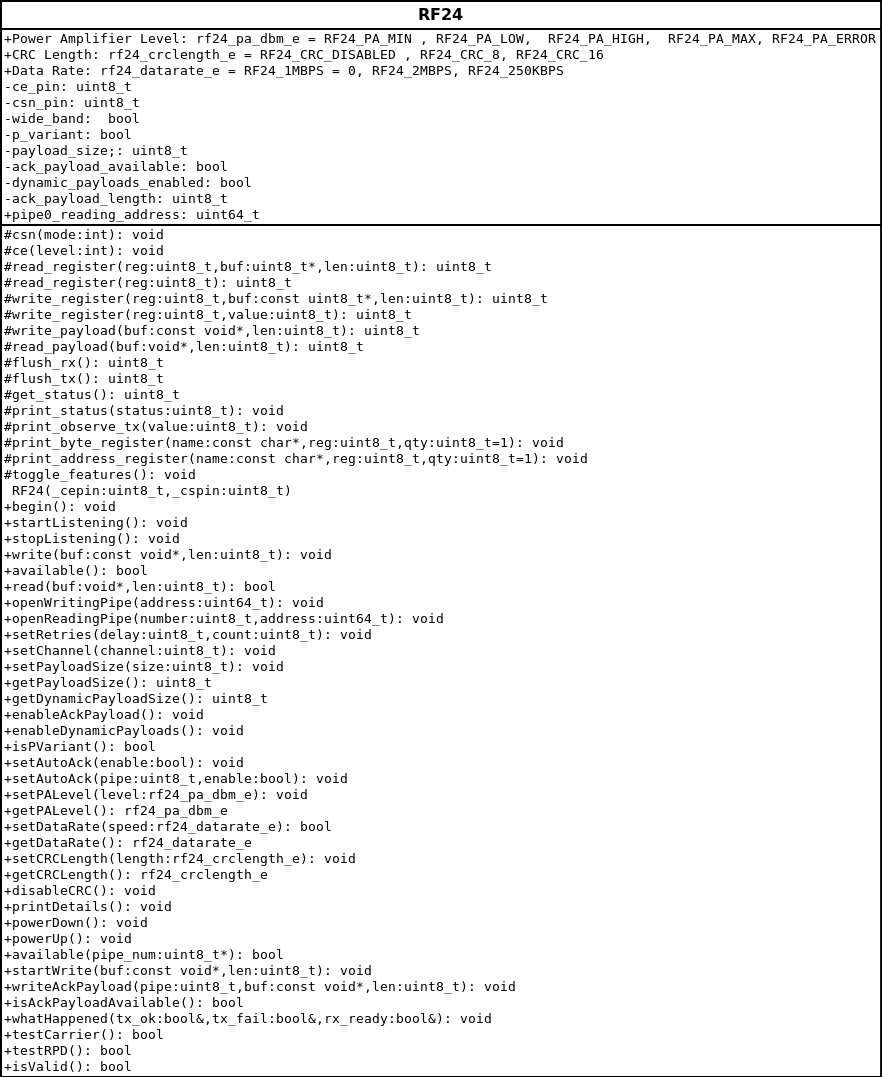
\includegraphics[width=\linewidth]{../../Imagens/RF24_class.png}
    \caption{Diagrama da Classe RF24} %% TODO certificar se realmente é uma WBS!!!
    \label{RF24_ClassDiag}
  \end{figure}

 \section{Estrutura Analítica do Projeto}
  \begin{figure}[H] %% TODO certificar se realmente é uma WBS!!!
    \centering
    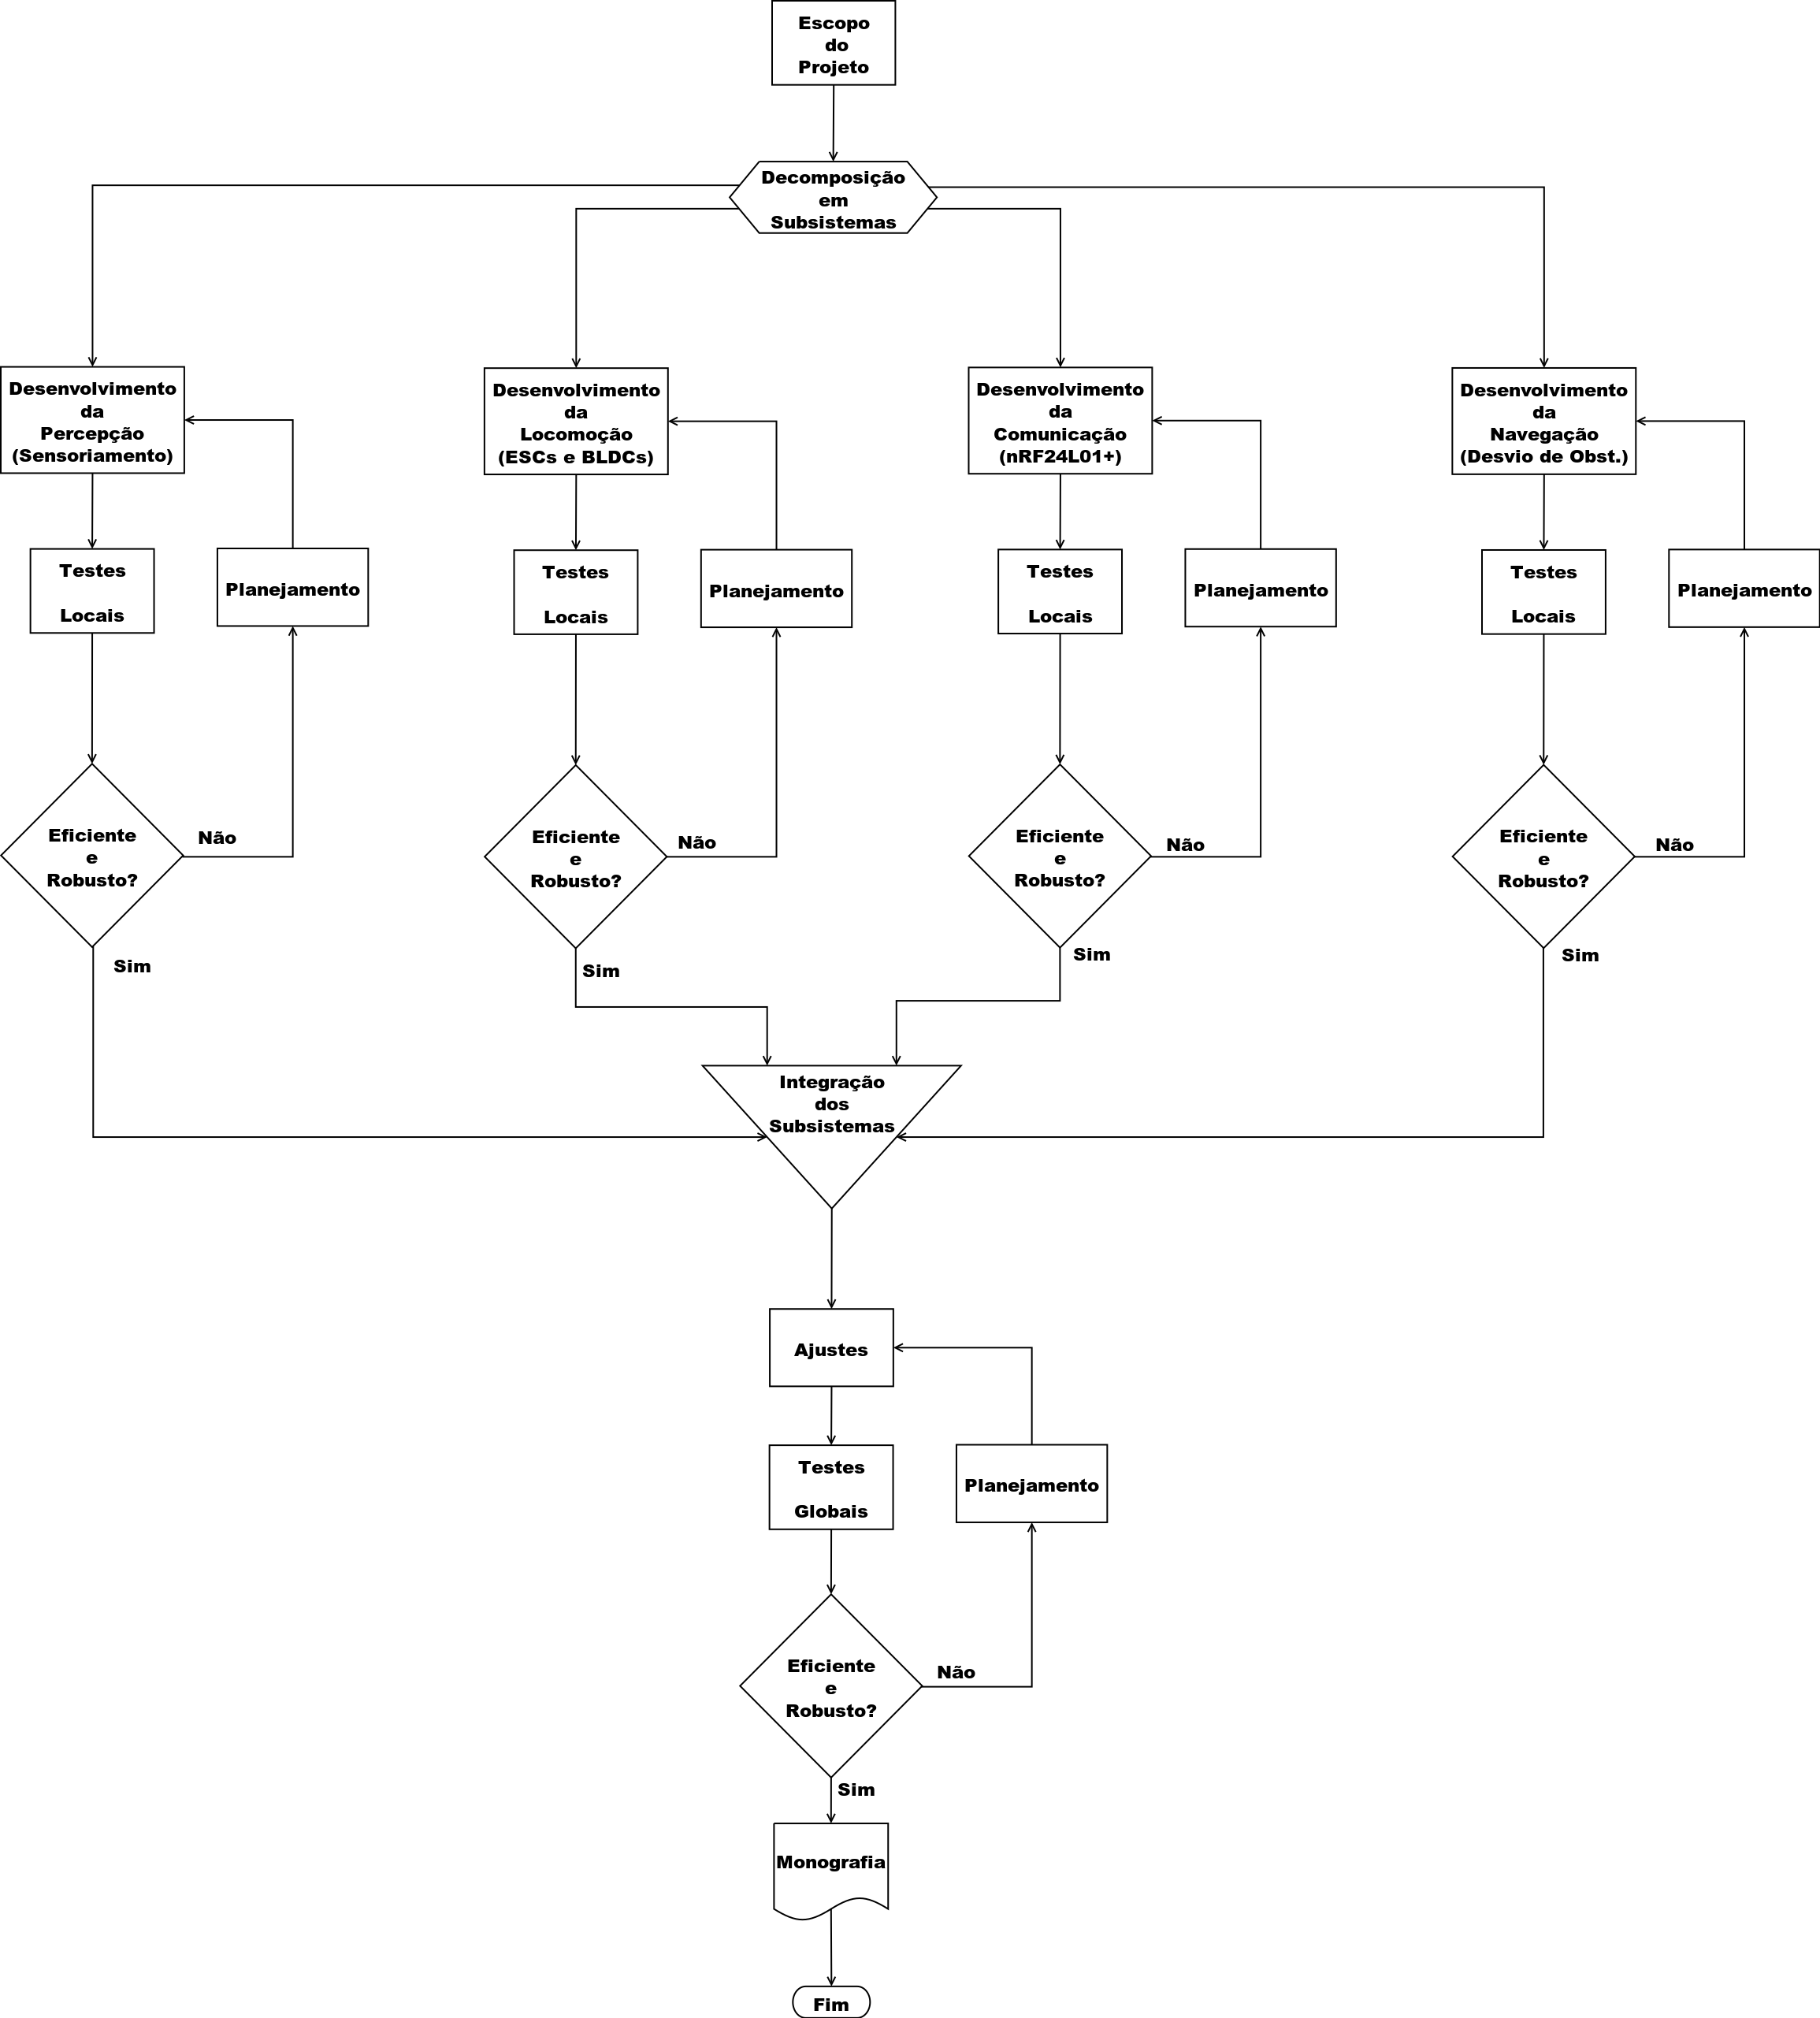
\includegraphics[width=\linewidth]{../../Imagens/WBS.png}
    \caption{Estrutura Analítica do Projeto} %% TODO certificar se realmente é uma WBS!!!
    \label{WBS}
  \end{figure}
  
 \section{Esquemático do Robô}
  \begin{figure}[H]
    \centering
    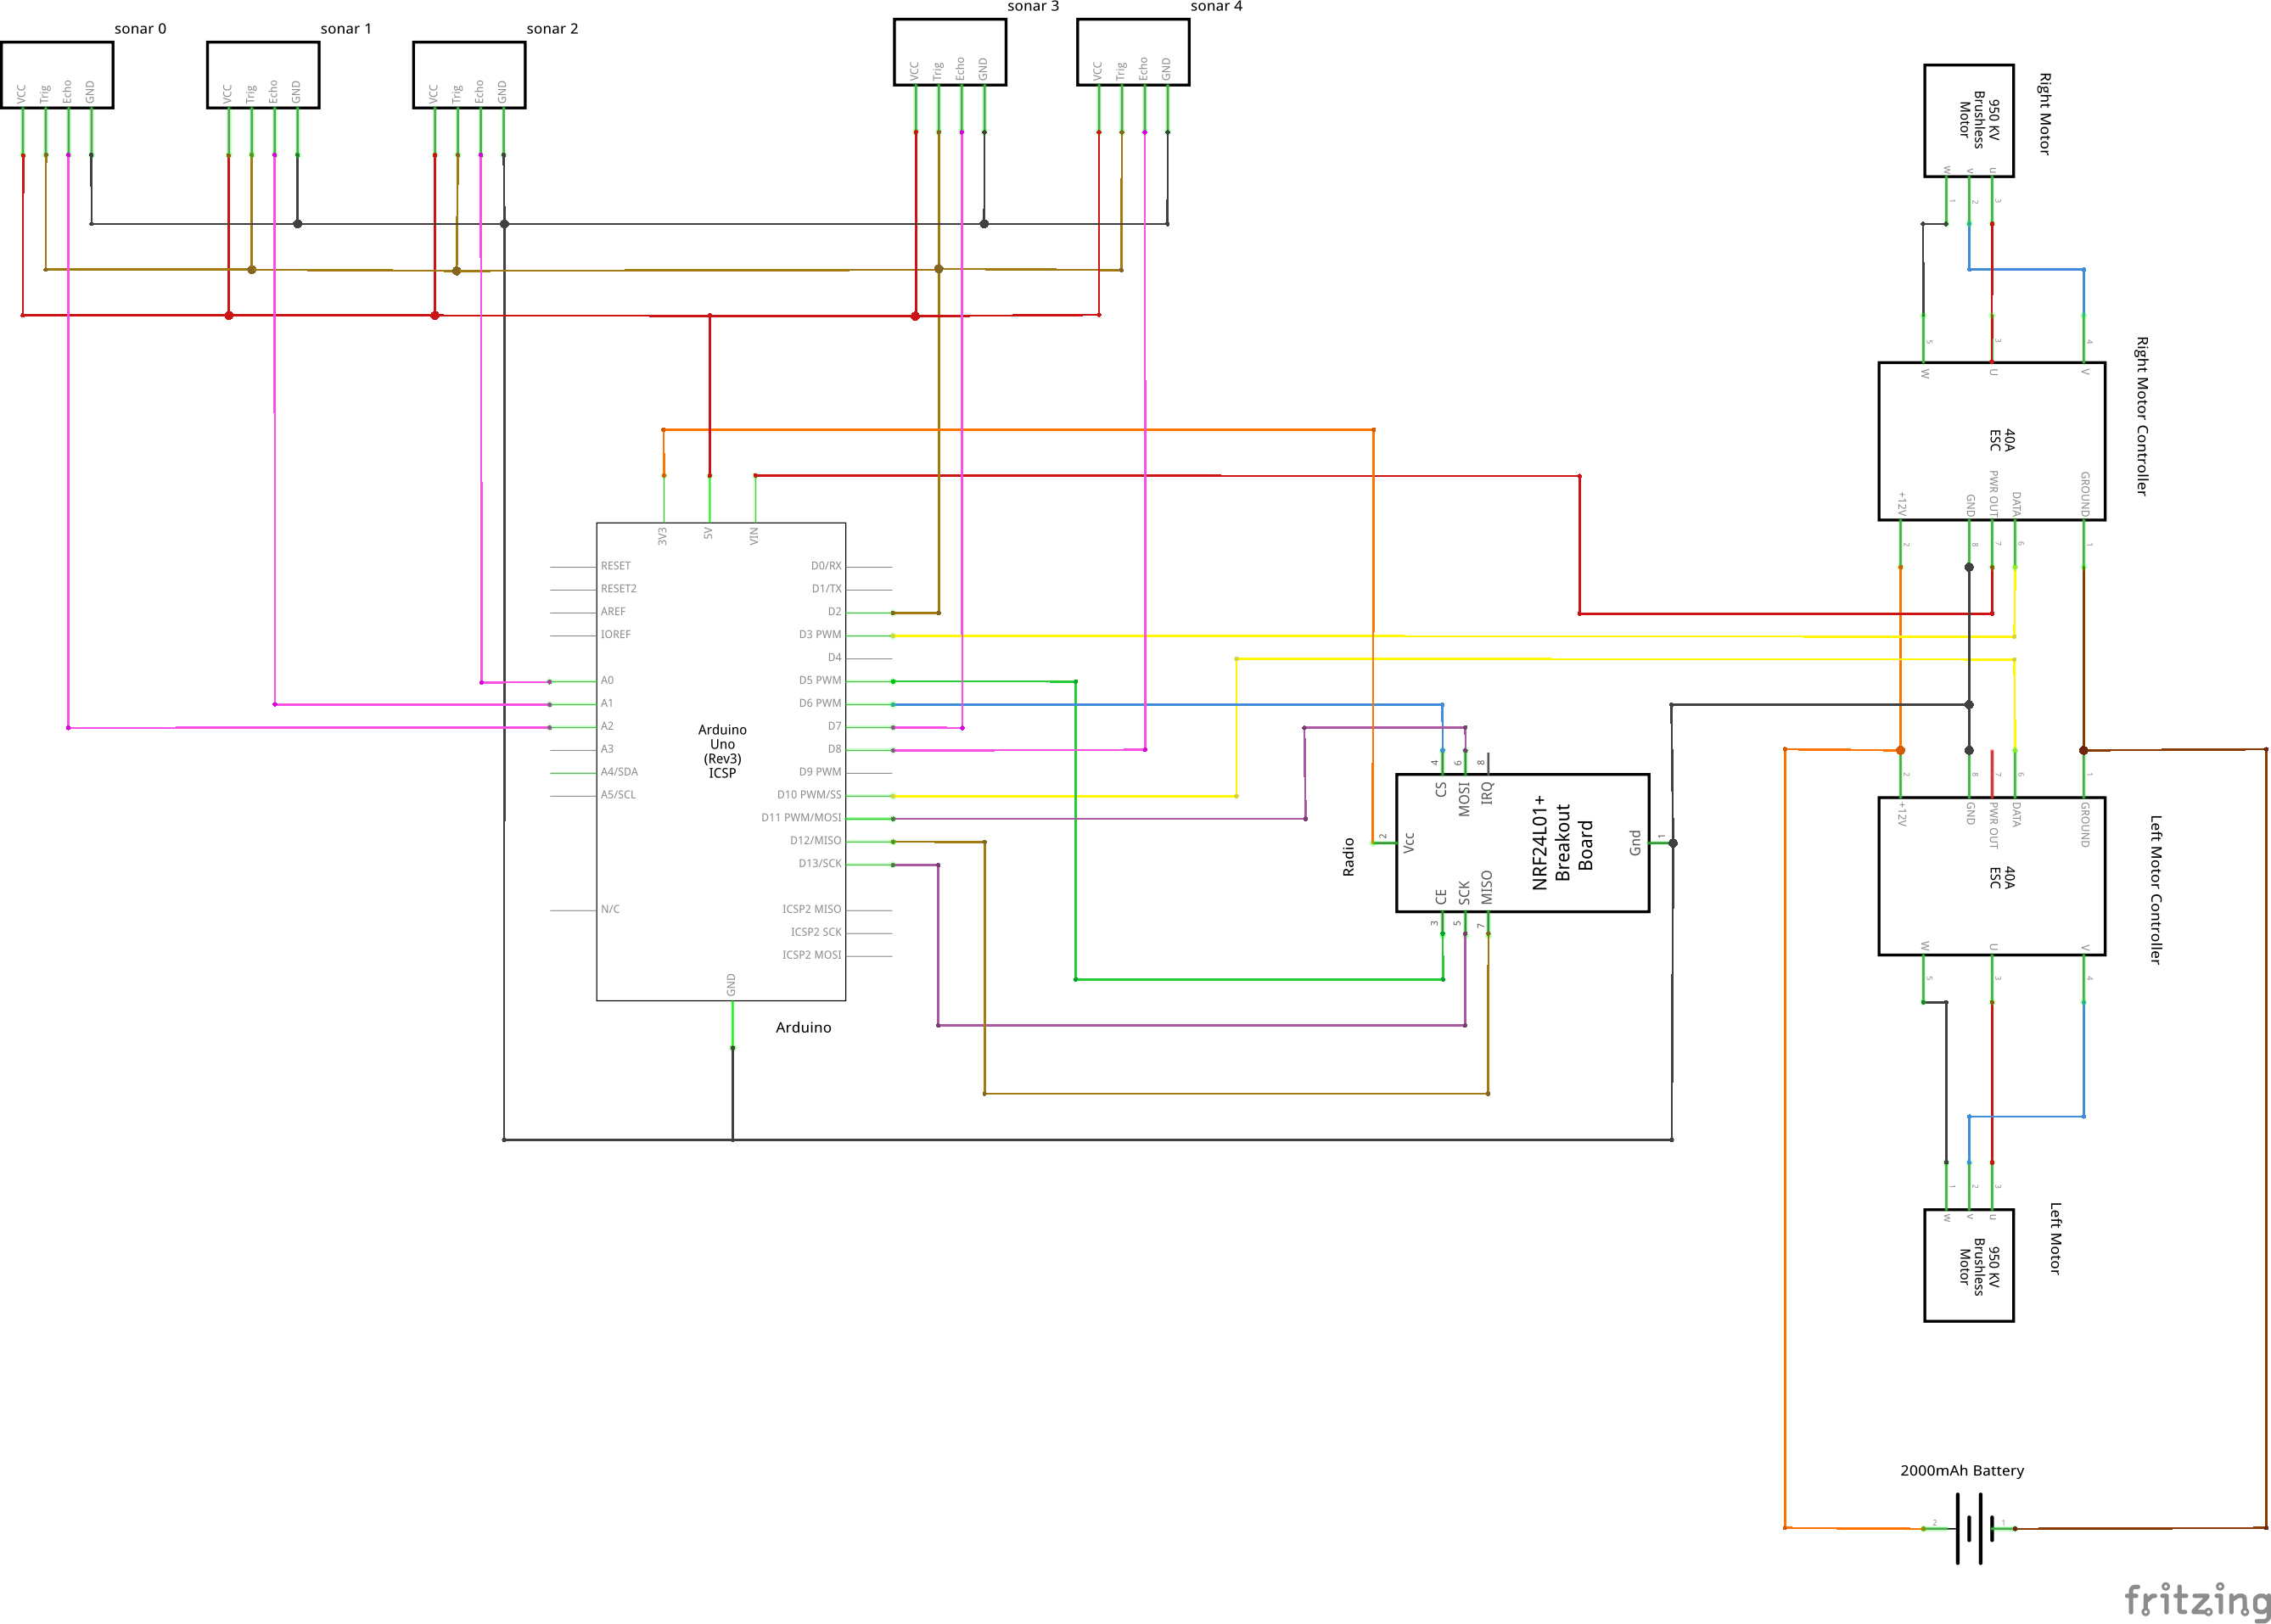
\includegraphics[width=\linewidth]{../../Imagens/robot_schem.png}
    \caption{Diagrama Elétrico} %% TODO: é um bom nome??
    \label{fritzing}
  \end{figure}
  
 \section{Testes}
 \subsection{Leituras Espúrias}
% Please add the following required packages to your document preamble:
% \usepackage{multirow}
\begin{table}[H]
\centering
\caption{Teste sem Obstáculos ao Alcance}
\label{vazio}
\begin{tabular}{|c|c|c|ccccc|}\hline
Dados & Contagem & Intervalo & Sensor 0 & Sensor 1 & Sensor 2 & Sensor 3 & Sensor 4 \\ \hline
\multirow{6}{*}{crus} & \multirow{3}{*}{$\neq 400$} & 30ms & 0\% & 1,22\% & 0\% & 1,48\% & 0\% \\
 &  & 45ms & 0,67\% & 0,92\% & 0\% & 1,58\% & 0\% \\
 &  & 60ms & 3,17\% & 0,58\% & 0\% & 2,67\% & 0\% \\ \cline{2-8} 
 & \multirow{3}{*}{\textless \hspace{0,5mm} 10} & 30ms & 0\% & 0\% & 0\% & 0,78\% & 0\% \\
 &  & 45ms & 0,67\% & 0\% & 0\% & 0,83\% & 0\% \\
 &  & 60ms & 3,17\% & 0\% & 0\% & 1,08\% & 0\% \\ \hline
\multirow{6}{*}{processados} & \multirow{3}{*}{$\neq 400$} & 30ms & 0\% & 0,70\% & 0\% & 0,35\% & 0\% \\
 &  & 45ms & 0\% & 0,25\% & 0\% & 0,33\% & 0\% \\
 &  & 60ms & 0\% & 0,08\% & 0\% & 1,09\% & 0\% \\ \cline{2-8} 
 & \multirow{3}{*}{\textless \hspace{0,5mm} 10} & 30ms & 0\% & 0\% & 0\% & 0\% & 0\% \\
 &  & 45ms & 0\% & 0\% & 0\% & 0\% & 0\% \\
 &  & 60ms & 0\% & 0\% & 0\% & 0\% & 0\% \\ \hline
\end{tabular}
\end{table}

  \pagebreak

 \subsection{Leituras Dinâmicas x Estáticas}
 % Please add the following required packages to your document preamble:
% \usepackage{multirow}
\begin{center}
\begin{longtable}{|c|c|c|ccccc|}
\label{30cm} \\
\caption[30cm]{30cm} \endfirsthead \\
\caption[]{30cm} \\
\hline \multicolumn{3}{|c|}{{Continua na próxima página.}} \\ \hline
\endfoot \hline
\hline \hline
\endlastfoot
\hline
\textbf{Medida} & \textbf{Intervalo} & \textbf{Leitura} & \textbf{Sensor 0} & \textbf{Sensor 1} & \textbf{Sensor 2} & \textbf{Sensor 3} & \textbf{Sensor 4} \\ \hline
\multirow{12}{*}{\begin{tabular}[c]{@{}c@{}}Média\\ {[}cm{]}\end{tabular}} & \multirow{4}{*}{30ms} & Est. & 26,43 & 30,13 & 31,14 & 35,62 & 37,19 \\
 &  & Din. & 26,58 & 30,57 & 30,55 & 35,67 & 37,51 \\
 &  & Est. & 26,37 & 30,12 & 30,99 & 35,66 & 37,21 \\
 &  & Din. & 26,42 & 30,60 & 32,17 & 35,61 & 37,52 \\ \cline{2-8} 
 & \multirow{4}{*}{45ms} & Est. & 26,36 & 30,51 & 32,61 & 35,67 & 37,34 \\
 &  & Din. & 26,39 & 30,86 & 32,31 & 35,76 & 37,73 \\
 &  & Est. & 26,45 & 30,26 & 31,59 & 35,75 & 37,17 \\
 &  & Din. & 26,42 & 30,29 & 29,11 & 35,65 & 37,36 \\ \cline{2-8} 
 & \multirow{4}{*}{60ms} & Est. & 26,41 & 30,12 & 31,28 & 35,67 & 37,21 \\
 &  & Din. & 26,72 & 30,48 & 31,11 & 35,71 & 37,65 \\
 &  & Est. & 26,46 & 30,01 & 30,38 & 35,61 & 37,15 \\
 &  & Din. & 26,52 & 30,35 & 28,47 & 35,50 & 37,33 \\ \hline
\multirow{12}{*}{\begin{tabular}[c]{@{}c@{}}Média\\ Limpa\\ {[}cm{]}\end{tabular}} & \multirow{4}{*}{30ms} & Est. & 26,43 & 30,13 & 31,14 & 35,62 & 37,19 \\
 &  & Din. & 26,58 & 30,57 & 31,16 & 35,67 & 37,51 \\
 &  & Est. & 26,37 & 30,12 & 30,99 & 35,66 & 37,21 \\
 &  & Din. & 26,42 & 30,60 & 32,69 & 35,61 & 37,52 \\ \cline{2-8} 
 & \multirow{4}{*}{45ms} & Est. & 26,36 & 30,51 & 32,61 & 35,67 & 37,34 \\
 &  & Din. & 26,39 & 30,86 & 32,82 & 35,76 & 37,73 \\
 &  & Est. & 26,45 & 30,26 & 31,59 & 35,75 & 37,17 \\
 &  & Din. & 26,42 & 30,29 & 31,91 & 35,65 & 37,36 \\ \cline{2-8} 
 & \multirow{4}{*}{60ms} & Est. & 26,41 & 30,12 & 31,28 & 35,67 & 37,21 \\
 &  & Din. & 26,72 & 30,48 & 31,59 & 35,71 & 37,65 \\
 &  & Est. & 26,46 & 30,01 & 30,38 & 35,61 & 37,15 \\
 &  & Din. & 26,52 & 30,35 & 30,84 & 35,50 & 37,33 \\ \hline \pagebreak
\multirow{12}{*}{\begin{tabular}[c]{@{}c@{}}Desvio\\ Padrão\\ {[}cm{]}\end{tabular}} & \multirow{4}{*}{30ms} & Est. & 0,50 & 0,34 & 1,51 & 0,49 & 0,41 \\
 &  & Din. & 0,50 & 0,50 & 4,19 & 0,55 & 0,53 \\
 &  & Est. & 0,48 & 0,33 & 1,19 & 0,48 & 0,43 \\
 &  & Din. & 0,50 & 0,49 & 4,35 & 0,59 & 0,55 \\ \cline{2-8} 
 & \multirow{4}{*}{45ms} & Est. & 0,48 & 0,50 & 1,68 & 0,47 & 0,52 \\
 &  & Din. & 0,49 & 0,35 & 4,12 & 0,54 & 0,62 \\
 &  & Est. & 0,50 & 0,44 & 1,63 & 0,44 & 0,41 \\
 &  & Din. & 0,50 & 0,46 & 8,18 & 0,48 & 0,63 \\ \cline{2-8} 
 & \multirow{4}{*}{60ms} & Est. & 0,49 & 0,33 & 1,42 & 0,47 & 0,41 \\
 &  & Din. & 0,45 & 0,50 & 4,10 & 0,50 & 0,69 \\
 &  & Est. & 0,50 & 0,12 & 0,70 & 0,49 & 0,38 \\
 &  & Din. & 0,50 & 0,48 & 7,47 & 0,50 & 0,49 \\ \hline
\multirow{12}{*}{\textless avg - 15} & \multirow{4}{*}{30ms} & Est. & 0,00\% & 0,00\% & 0,00\% & 0,00\% & 0,00\% \\
 &  & Din. & 0,00\% & 0,00\% & 2,67\% & 0,00\% & 0,00\% \\
 &  & Est. & 0,00\% & 0,00\% & 0,00\% & 0,00\% & 0,00\% \\
 &  & Din. & 0,00\% & 0,00\% & 2,00\% & 0,00\% & 0,00\% \\ \cline{2-8} 
 & \multirow{4}{*}{45ms} & Est. & 0,00\% & 0,00\% & 0,00\% & 0,00\% & 0,00\% \\
 &  & Din. & 0,00\% & 0,00\% & 2,00\% & 0,00\% & 0,00\% \\
 &  & Est. & 0,00\% & 0,00\% & 0,00\% & 0,00\% & 0,00\% \\
 &  & Din. & 0,00\% & 0,00\% & 11,33\% & 0,00\% & 0,00\% \\ \cline{2-8} 
 & \multirow{4}{*}{60ms} & Est. & 0,00\% & 0,00\% & 0,00\% & 0,00\% & 0,00\% \\
 &  & Din. & 0,00\% & 0,00\% & 2,00\% & 0,00\% & 0,00\% \\
 &  & Est. & 0,00\% & 0,00\% & 0,00\% & 0,00\% & 0,00\% \\
 &  & Din. & 0,00\% & 0,00\% & 10,00\% & 0,00\% & 0,00\% \\ \hline
\multirow{12}{*}{\textgreater avg + 15} & \multirow{4}{*}{30ms} & Est. & 0,00\% & 0,00\% & 1,33\% & 0,00\% & 0,00\% \\
 &  & Din. & 0,00\% & 0,00\% & 4,00\% & 0,00\% & 0,00\% \\
 &  & Est. & 0,00\% & 0,00\% & 0,67\% & 0,00\% & 0,00\% \\
 &  & Din. & 0,00\% & 0,00\% & 4,67\% & 0,00\% & 0,00\% \\ \cline{2-8} 
 & \multirow{4}{*}{45ms} & Est. & 0,00\% & 0,00\% & 0,00\% & 0,00\% & 0,00\% \\
 &  & Din. & 0,00\% & 0,00\% & 1,33\% & 0,00\% & 0,00\% \\
 &  & Est. & 0,00\% & 0,00\% & 0,00\% & 0,00\% & 0,00\% \\
 &  & Din. & 0,00\% & 0,00\% & 6,67\% & 0,00\% & 0,00\% \\ \cline{2-8} 
 & \multirow{4}{*}{60ms} & Est. & 0,00\% & 0,00\% & 0,00\% & 0,00\% & 0,00\% \\
 &  & Din. & 0,00\% & 0,00\% & 7,33\% & 0,00\% & 0,00\% \\
 &  & Est. & 0,00\% & 0,00\% & 0,00\% & 0,00\% & 0,00\% \\
 &  & Din. & 0,00\% & 0,00\% & 6,67\% & 0,00\% & 0,00\% \\ \hline
\multirow{12}{*}{= 400} & \multirow{4}{*}{30ms} & Est. & 0,00\% & 0,00\% & 0,00\% & 0,00\% & 0,00\% \\
 &  & Din. & 0,00\% & 0,00\% & 0,00\% & 0,00\% & 0,00\% \\
 &  & Est. & 0,00\% & 0,00\% & 0,00\% & 0,00\% & 0,00\% \\
 &  & Din. & 0,00\% & 0,00\% & 0,00\% & 0,00\% & 0,00\% \\ \cline{2-8} 
 & \multirow{4}{*}{45ms} & Est. & 0,00\% & 0,00\% & 0,00\% & 0,00\% & 0,00\% \\
 &  & Din. & 0,00\% & 0,00\% & 0,00\% & 0,00\% & 0,00\% \\
 &  & Est. & 0,00\% & 0,00\% & 0,00\% & 0,00\% & 0,00\% \\
 &  & Din. & 0,00\% & 0,00\% & 0,00\% & 0,00\% & 0,00\% \\ \cline{2-8} 
 & \multirow{4}{*}{60ms} & Est. & 0,00\% & 0,00\% & 0,00\% & 0,00\% & 0,00\% \\
 &  & Din. & 0,00\% & 0,00\% & 0,00\% & 0,00\% & 0,00\% \\
 &  & Est. & 0,00\% & 0,00\% & 0,00\% & 0,00\% & 0,00\% \\
 &  & Din. & 0,00\% & 0,00\% & 0,00\% & 0,00\% & 0,00\% \\ \hline
\end{longtable}
\end{center}

  % Please add the following required packages to your document preamble:
% \usepackage{multirow}
\begin{center}
\begin{longtable}{|c|c|c|ccccc|}
\label{50cm} \\
\caption[50cm]{50cm} \endfirsthead \\
\caption[]{50cm} \\
\hline \multicolumn{3}{|c|}{{Continua na próxima página.}} \\ \hline
\endfoot \hline
\hline \hline
\endlastfoot
\hline
\textbf{Medida} & \textbf{Intervalo} & \textbf{Leitura} & \textbf{Sensor 0} & \textbf{Sensor 1} & \textbf{Sensor 2} & \textbf{Sensor 3} & \textbf{Sensor 4} \\ \hline
\multirow{12}{*}{\begin{tabular}[c]{@{}c@{}}Média\\ {[}cm{]}\end{tabular}} & \multirow{4}{*}{30ms} & Est. & 44,80 & 47,77 & 50,86 & 48,39 & 53,25 \\
 &  & Din. & 44,57 & 47,87 & 50,13 & 48,59 & 53,65 \\
 &  & Est. & 45,21 & 47,91 & 50,86 & 48,35 & 52,49 \\
 &  & Din. & 44,95 & 47,83 & 50,65 & 48,77 & 52,65 \\ \cline{2-8} 
 & \multirow{4}{*}{45ms} & Est. & 45,35 & 47,46 & 50,45 & 48,53 & 53,61 \\
 &  & Din. & 44,85 & 47,85 & 52,61 & 48,92 & 63,21 \\
 &  & Est. & 44,70 & 47,72 & 51,35 & 48,56 & 53,06 \\
 &  & Din. & 44,79 & 47,91 & 50,87 & 48,67 & 60,42 \\ \cline{2-8} 
 & \multirow{4}{*}{60ms} & Est. & 45,86 & 47,76 & 50,81 & 48,49 & 51,69 \\
 &  & Din. & 45,27 & 47,85 & 50,74 & 48,94 & 52,55 \\
 &  & Est. & 45,68 & 47,89 & 51,54 & 48,61 & 53,26 \\
 &  & Din. & 44,78 & 47,63 & 51,29 & 48,73 & 51,33 \\ \hline  \pagebreak
\multirow{12}{*}{\begin{tabular}[c]{@{}c@{}}Média\\ Limpa\\ {[}cm{]}\end{tabular}} & \multirow{4}{*}{30ms} & Est. & 44,80 & 47,77 & 50,86 & 48,39 & 53,25 \\
 &  & Din. & 44,57 & 47,87 & 50,13 & 48,59 & 53,65 \\
 &  & Est. & 45,21 & 47,91 & 50,86 & 48,35 & 52,49 \\
 &  & Din. & 44,95 & 47,83 & 50,65 & 48,77 & 52,65 \\ \cline{2-8} 
 & \multirow{4}{*}{45ms} & Est. & 45,35 & 47,46 & 50,45 & 48,53 & 53,61 \\
 &  & Din. & 44,85 & 47,85 & 52,61 & 48,92 & 63,21 \\
 &  & Est. & 44,70 & 47,72 & 51,35 & 48,56 & 53,06 \\
 &  & Din. & 44,79 & 47,91 & 50,87 & 48,67 & 60,42 \\ \cline{2-8} 
 & \multirow{4}{*}{60ms} & Est. & 45,86 & 47,76 & 50,81 & 48,49 & 51,69 \\
 &  & Din. & 45,27 & 47,85 & 50,74 & 48,94 & 52,55 \\
 &  & Est. & 45,68 & 47,89 & 51,54 & 48,61 & 53,26 \\
 &  & Din. & 44,78 & 47,63 & 51,29 & 48,73 & 51,33 \\ \hline
\multirow{12}{*}{\begin{tabular}[c]{@{}c@{}}Desvio\\ Padrão\\ {[}cm{]}\end{tabular}} & \multirow{4}{*}{30ms} & Est. & 0,65 & 0,42 & 0,74 & 0,50 & 11,99 \\
 &  & Din. & 0,56 & 0,33 & 1,48 & 0,53 & 12,93 \\
 &  & Est. & 2,96 & 0,29 & 0,74 & 0,48 & 11,24 \\
 &  & Din. & 1,00 & 0,37 & 1,17 & 0,49 & 11,11 \\ \cline{2-8} 
 & \multirow{4}{*}{45ms} & Est. & 3,38 & 0,50 & 0,97 & 0,51 & 13,46 \\
 &  & Din. & 0,63 & 0,36 & 1,16 & 0,54 & 28,66 \\
 &  & Est. & 0,76 & 0,45 & 0,81 & 0,50 & 12,03 \\
 &  & Din. & 0,53 & 0,28 & 0,70 & 0,51 & 26,26 \\ \cline{2-8} 
 & \multirow{4}{*}{60ms} & Est. & 7,40 & 0,43 & 0,87 & 0,50 & 7,44 \\
 &  & Din. & 2,98 & 0,35 & 0,81 & 0,48 & 8,89 \\
 &  & Est. & 6,25 & 0,31 & 0,81 & 0,50 & 11,92 \\
 &  & Din. & 0,53 & 0,48 & 1,30 & 0,49 & 5,41 \\ \hline
\multirow{12}{*}{\textless avg - 15} & \multirow{4}{*}{30ms} & Est. & 0,00\% & 0,00\% & 0,00\% & 0,00\% & 0,00\% \\
 &  & Din. & 0,00\% & 0,00\% & 0,00\% & 0,00\% & 0,00\% \\
 &  & Est. & 0,00\% & 0,00\% & 0,00\% & 0,00\% & 0,00\% \\
 &  & Din. & 0,00\% & 0,00\% & 0,00\% & 0,00\% & 0,00\% \\ \cline{2-8} 
 & \multirow{4}{*}{45ms} & Est. & 0,00\% & 0,00\% & 0,00\% & 0,00\% & 0,00\% \\
 &  & Din. & 0,00\% & 0,00\% & 0,00\% & 0,00\% & 0,00\% \\
 &  & Est. & 0,00\% & 0,00\% & 0,00\% & 0,00\% & 0,00\% \\
 &  & Din. & 0,00\% & 0,00\% & 0,00\% & 0,00\% & 0,00\% \\ \cline{2-8} 
 & \multirow{4}{*}{60ms} & Est. & 0,00\% & 0,00\% & 0,00\% & 0,00\% & 0,00\% \\
 &  & Din. & 0,00\% & 0,00\% & 0,00\% & 0,00\% & 0,00\% \\
 &  & Est. & 0,00\% & 0,00\% & 0,00\% & 0,00\% & 0,00\% \\
 &  & Din. & 0,00\% & 0,00\% & 0,00\% & 0,00\% & 0,00\% \\ \hline
\multirow{12}{*}{\textgreater avg + 15} & \multirow{4}{*}{30ms} & Est. & 0,00\% & 0,00\% & 0,00\% & 0,00\% & 4,00\% \\
 &  & Din. & 0,00\% & 0,00\% & 0,00\% & 0,00\% & 5,33\% \\
 &  & Est. & 0,67\% & 0,00\% & 0,00\% & 0,00\% & 2,67\% \\
 &  & Din. & 0,00\% & 0,00\% & 0,00\% & 0,00\% & 2,67\% \\ \cline{2-8} 
 & \multirow{4}{*}{45ms} & Est. & 0,67\% & 0,00\% & 0,00\% & 0,00\% & 4,00\% \\
 &  & Din. & 0,00\% & 0,00\% & 0,00\% & 0,00\% & 16,00\% \\
 &  & Est. & 0,00\% & 0,00\% & 0,00\% & 0,00\% & 3,33\% \\
 &  & Din. & 0,00\% & 0,00\% & 0,00\% & 0,00\% & 12,67\% \\ \cline{2-8} 
 & \multirow{4}{*}{60ms} & Est. & 1,33\% & 0,00\% & 0,00\% & 0,00\% & 1,33\% \\
 &  & Din. & 0,67\% & 0,00\% & 0,00\% & 0,00\% & 2,67\% \\
 &  & Est. & 1,33\% & 0,00\% & 0,00\% & 0,00\% & 4,67\% \\
 &  & Din. & 0,00\% & 0,00\% & 0,00\% & 0,00\% & 0,67\% \\ \hline
\multirow{12}{*}{= 400} & \multirow{4}{*}{30ms} & Est. & 0,00\% & 0,00\% & 0,00\% & 0,00\% & 0,00\% \\
 &  & Din. & 0,00\% & 0,00\% & 0,00\% & 0,00\% & 0,00\% \\
 &  & Est. & 0,00\% & 0,00\% & 0,00\% & 0,00\% & 0,00\% \\
 &  & Din. & 0,00\% & 0,00\% & 0,00\% & 0,00\% & 0,00\% \\ \cline{2-8} 
 & \multirow{4}{*}{45ms} & Est. & 0,00\% & 0,00\% & 0,00\% & 0,00\% & 0,00\% \\
 &  & Din. & 0,00\% & 0,00\% & 0,00\% & 0,00\% & 0,00\% \\
 &  & Est. & 0,00\% & 0,00\% & 0,00\% & 0,00\% & 0,00\% \\
 &  & Din. & 0,00\% & 0,00\% & 0,00\% & 0,00\% & 0,00\% \\ \cline{2-8} 
 & \multirow{4}{*}{60ms} & Est. & 0,00\% & 0,00\% & 0,00\% & 0,00\% & 0,00\% \\
 &  & Din. & 0,00\% & 0,00\% & 0,00\% & 0,00\% & 0,00\% \\
 &  & Est. & 0,00\% & 0,00\% & 0,00\% & 0,00\% & 0,00\% \\
 &  & Din. & 0,00\% & 0,00\% & 0,00\% & 0,00\% & 0,00\% \\ \hline
\end{longtable}
\end{center}

\pagebreak
  % Please add the following required packages to your document preamble:
% \usepackage{multirow}
\begin{center}
\begin{longtable}{|c|c|c|ccccc|}
\label{100cm} \\
\caption[100cm]{100cm} \endfirsthead \\
\caption[]{100cm} \\
\hline \multicolumn{3}{|c|}{{Continua na próxima página.}} \\ \hline
\endfoot \hline
\hline \hline
\endlastfoot
\hline
\textbf{Medida} & \textbf{Intervalo} & \textbf{Leitura} & \textbf{Sensor 0} & \textbf{Sensor 1} & \textbf{Sensor 2} & \textbf{Sensor 3} & \textbf{Sensor 4} \\ \hline
\multirow{12}{*}{\begin{tabular}[c]{@{}c@{}}Média\\ {[}cm{]}\end{tabular}} & \multirow{4}{*}{30ms} & Est. & 102,49 & 106,83 & 96,83 & 92,05 & 94,19 \\
 &  & Din. & 102,71 & 107,05 & 97,07 & 92,46 & 94,74 \\
 &  & Est. & 102,41 & 106,85 & 96,83 & 92,21 & 94,49 \\
 &  & Din. & 102,46 & 106,91 & 97,19 & 92,54 & 94,54 \\ \cline{2-8} 
 & \multirow{4}{*}{45ms} & Est. & 102,78 & 106,86 & 96,96 & 92,05 & 94,29 \\
 &  & Din. & 102,31 & 106,82 & 97,10 & 92,37 & 94,49 \\
 &  & Est. & 102,41 & 106,89 & 97,07 & 92,20 & 94,27 \\
 &  & Din. & 102,37 & 106,83 & 97,07 & 92,23 & 94,20 \\ \cline{2-8} 
 & \multirow{4}{*}{60ms} & Est. & 102,63 & 106,96 & 97,46 & 92,14 & 94,24 \\
 &  & Din. & 102,34 & 106,81 & 97,23 & 92,46 & 94,53 \\
 &  & Est. & 102,59 & 106,90 & 97,07 & 92,43 & 94,60 \\
 &  & Din. & 102,07 & 106,77 & 97,18 & 92,51 & 94,65 \\ \hline
\multirow{12}{*}{\begin{tabular}[c]{@{}c@{}}Média\\ Limpa\\ {[}cm{]}\end{tabular}} & \multirow{4}{*}{30ms} & Est. & 102,49 & 106,83 & 96,83 & 92,05 & 94,19 \\
 &  & Din. & 102,71 & 107,05 & 97,07 & 92,46 & 94,74 \\
 &  & Est. & 102,41 & 106,85 & 96,83 & 92,21 & 94,49 \\
 &  & Din. & 102,46 & 106,91 & 97,19 & 92,54 & 94,54 \\ \cline{2-8} 
 & \multirow{4}{*}{45ms} & Est. & 102,78 & 106,86 & 96,96 & 92,05 & 94,29 \\
 &  & Din. & 102,31 & 106,82 & 97,10 & 92,37 & 94,49 \\
 &  & Est. & 102,41 & 106,89 & 97,07 & 92,20 & 94,27 \\
 &  & Din. & 102,37 & 106,83 & 97,07 & 92,23 & 94,20 \\ \cline{2-8} 
 & \multirow{4}{*}{60ms} & Est. & 102,63 & 106,96 & 97,46 & 92,14 & 94,24 \\
 &  & Din. & 102,34 & 106,81 & 97,23 & 92,46 & 94,53 \\
 &  & Est. & 102,59 & 106,90 & 97,07 & 92,43 & 94,60 \\
 &  & Din. & 102,07 & 106,77 & 97,18 & 92,51 & 94,65 \\ \hline
\multirow{12}{*}{\begin{tabular}[c]{@{}c@{}}Desvio\\ Padrão\\ {[}cm{]}\end{tabular}} & \multirow{4}{*}{30ms} & Est. & 0,66 & 0,39 & 0,78 & 0,24 & 1,02 \\
 &  & Din. & 0,99 & 0,44 & 0,73 & 0,53 & 1,12 \\
 &  & Est. & 0,66 & 0,38 & 0,77 & 0,41 & 1,01 \\
 &  & Din. & 0,66 & 0,29 & 0,75 & 0,57 & 0,98 \\ \cline{2-8} 
 & \multirow{4}{*}{45ms} & Est. & 0,83 & 0,35 & 0,72 & 0,33 & 1,01 \\
 &  & Din. & 0,60 & 0,39 & 0,78 & 0,56 & 0,99 \\
 &  & Est. & 0,66 & 0,31 & 0,77 & 0,42 & 0,83 \\
 &  & Din. & 0,66 & 0,40 & 0,81 & 0,44 & 0,62 \\ \cline{2-8}  \pagebreak
 & \multirow{4}{*}{60ms} & Est. & 0,69 & 0,33 & 2,52 & 0,37 & 1,07 \\
 &  & Din. & 0,61 & 0,39 & 0,76 & 0,54 & 0,95 \\
 &  & Est. & 0,73 & 0,34 & 0,72 & 0,50 & 1,22 \\
 &  & Din. & 0,53 & 0,42 & 0,71 & 0,58 & 0,99 \\ \hline
\multirow{12}{*}{\textless avg - 15} & \multirow{4}{*}{30ms} & Est. &0\% &0\% &0\% &0\% &0\% \\
 &  & Din. &0\% &0\% &0\% &0\% &0\% \\
 &  & Est. &0\% &0\% &0\% &0\% &0\% \\
 &  & Din. &0\% &0\% &0\% &0\% &0\% \\ \cline{2-8} 
 & \multirow{4}{*}{45ms} & Est. &0\% &0\% &0\% &0\% &0\% \\
 &  & Din. &0\% &0\% &0\% &0\% &0\% \\
 &  & Est. &0\% &0\% &0\% &0\% &0\% \\
 &  & Din. &0\% &0\% &0\% &0\% &0\% \\ \cline{2-8} 
 & \multirow{4}{*}{60ms} & Est. &0\% &0\% &0\% &0\% &0\% \\
 &  & Din. &0\% &0\% &0\% &0\% &0\% \\
 &  & Est. &0\% &0\% &0\% &0\% &0\% \\
 &  & Din. &0\% &0\% &0\% &0\% &0\% \\ \hline
\multirow{12}{*}{\textgreater avg + 15} & \multirow{4}{*}{30ms} & Est. &0\% &0\% &0\% &0\% &0\% \\
 &  & Din. &0\% &0\% &0\% &0\% &0\% \\
 &  & Est. &0\% &0\% &0\% &0\% &0\% \\
 &  & Din. &0\% &0\% &0\% &0\% &0\% \\ \cline{2-8} 
 & \multirow{4}{*}{45ms} & Est. &0\% &0\% &0\% &0\% &0\% \\
 &  & Din. &0\% &0\% &0\% &0\% &0\% \\
 &  & Est. &0\% &0\% &0\% &0\% &0\% \\
 &  & Din. &0\% &0\% &0\% &0\% &0\% \\ \cline{2-8} 
 & \multirow{4}{*}{60ms} & Est. &0\% &0\% & 0,67\% &0\% &0\% \\
 &  & Din. &0\% &0\% &0\% &0\% &0\% \\
 &  & Est. &0\% &0\% &0\% &0\% &0\% \\
 &  & Din. &0\% &0\% &0\% &0\% &0\% \\ \hline
\multirow{12}{*}{= 400} & \multirow{4}{*}{30ms} & Est. &0\% &0\% &0\% &0\% &0\% \\
 &  & Din. &0\% &0\% &0\% &0\% &0\% \\
 &  & Est. &0\% &0\% &0\% &0\% &0\% \\
 &  & Din. &0\% &0\% &0\% &0\% &0\% \\ \cline{2-8} 
 & \multirow{4}{*}{45ms} & Est. &0\% &0\% &0\% &0\% &0\% \\
 &  & Din. &0\% &0\% &0\% &0\% &0\% \\
 &  & Est. &0\% &0\% &0\% &0\% &0\% \\
 &  & Din. &0\% &0\% &0\% &0\% &0\% \\ \cline{2-8} 
 & \multirow{4}{*}{60ms} & Est. &0\% &0\% &0\% &0\% &0\% \\
 &  & Din. &0\% &0\% &0\% &0\% &0\% \\
 &  & Est. &0\% &0\% &0\% &0\% &0\% \\
 &  & Din. &0\% &0\% &0\% &0\% &0\% \\ \hline
\end{longtable}
\end{center}

  % Please add the following required packages to your document preamble:
% \usepackage{multirow}
\begin{center}
\begin{longtable}{|c|c|c|ccccc|}
\label{150cm} \\
\caption[150cm]{150cm} \endfirsthead \\
\caption[]{150cm} \\
\hline \multicolumn{3}{|c|}{{Continua na próxima página.}} \\ \hline
\endfoot \hline
\hline \hline
\endlastfoot
\hline
\textbf{Medida} & \textbf{Intervalo} & \textbf{Leitura} & \textbf{Sensor 0} & \textbf{Sensor 1} & \textbf{Sensor 2} & \textbf{Sensor 3} & \textbf{Sensor 4} \\ \hline
\multirow{12}{*}{\begin{tabular}[c]{@{}c@{}}Média\\ {[}cm{]}\end{tabular}} & \multirow{4}{*}{30ms} & Est. & 148,52 & 152,17 & 152,97 & 156,65 & 230,77 \\
 &  & Din. & 148,70 & 153,18 & 153,45 & 156,41 & 174,46 \\
 &  & Est. & 148,97 & 153,53 & 153,65 & 156,53 & 196,81 \\
 &  & Din. & 149,05 & 153,01 & 153,63 & 156,95 & 176,01 \\ \cline{2-8} 
 & \multirow{4}{*}{45ms} & Est. & 149,13 & 153,13 & 153,95 & 156,42 & 184,03 \\
 &  & Din. & 148,62 & 153,01 & 153,10 & 156,97 & 226,32 \\
 &  & Est. & 148,63 & 151,45 & 153,23 & 157,11 & 210,04 \\
 &  & Din. & 148,90 & 153,04 & 154,24 & 157,13 & 192,36 \\ \cline{2-8} 
 & \multirow{4}{*}{60ms} & Est. & 148,84 & 153,09 & 153,42 & 156,79 & 256,77 \\
 &  & Din. & 148,53 & 152,96 & 153,33 & 157,28 & 161,61 \\
 &  & Est. & 148,49 & 152,95 & 153,03 & 156,81 & 164,53 \\
 &  & Din. & 148,45 & 152,57 & 152,18 & 156,33 & 229,58 \\ \hline \multirow{12}{*}{\begin{tabular}[c]{@{}c@{}}Média\\ Limpa\\ {[}cm{]}\end{tabular}} & \multirow{4}{*}{30ms} & Est. & 148,52 & 152,17 & 152,97 & 156,65 & 158,25 \\
 &  & Din. & 148,70 & 153,18 & 153,45 & 156,41 & 158,35 \\
 &  & Est. & 148,97 & 153,53 & 153,65 & 156,53 & 158,10 \\
 &  & Din. & 149,05 & 153,01 & 153,63 & 156,95 & 158,28 \\ \cline{2-8} 
 & \multirow{4}{*}{45ms} & Est. & 149,13 & 153,13 & 153,95 & 156,42 & 158,25 \\
 &  & Din. & 148,62 & 153,01 & 153,10 & 156,97 & 158,78 \\
 &  & Est. & 148,63 & 151,45 & 153,23 & 157,11 & 158,53 \\
 &  & Din. & 148,90 & 153,04 & 154,24 & 157,13 & 158,56 \\ \cline{2-8} 
 & \multirow{4}{*}{60ms} & Est. & 148,84 & 153,09 & 153,42 & 156,79 & 158,60 \\
 &  & Din. & 148,53 & 152,96 & 153,33 & 157,28 & 158,39 \\
 &  & Est. & 148,49 & 152,95 & 153,03 & 156,81 & 158,08 \\
 &  & Din. & 148,45 & 152,57 & 152,18 & 156,33 & 158,84 \\ \hline \pagebreak
\multirow{12}{*}{\begin{tabular}[c]{@{}c@{}}Desvio\\ Padrão\\ {[}cm{]}\end{tabular}} & \multirow{4}{*}{30ms} & Est. & 0,60 & 7,48 & 6,44 & 0,76 & 111,16 \\
 &  & Din. & 0,63 & 0,39 & 0,64 & 0,88 & 60,49 \\
 &  & Est. & 0,52 & 0,50 & 0,65 & 0,68 & 88,98 \\
 &  & Din. & 0,47 & 0,08 & 0,61 & 0,68 & 63,23 \\ \cline{2-8} 
 & \multirow{4}{*}{45ms} & Est. & 0,42 & 0,33 & 0,73 & 0,74 & 74,88 \\
 &  & Din. & 0,63 & 0,23 & 0,86 & 0,82 & 108,67 \\
 &  & Est. & 0,61 & 9,46 & 0,89 & 0,64 & 99,26 \\
 &  & Din. & 0,47 & 0,30 & 6,01 & 0,72 & 84,06 \\ \cline{2-8} 
 & \multirow{4}{*}{60ms} & Est. & 0,57 & 0,28 & 0,63 & 0,57 & 118,98 \\
 &  & Din. & 0,62 & 0,20 & 0,62 & 0,65 & 27,81 \\
 &  & Est. & 0,54 & 0,21 & 0,68 & 0,61 & 39,11 \\
 &  & Din. & 0,59 & 4,90 & 5,68 & 0,89 & 110,18 \\ \hline
\multirow{12}{*}{\textless avg - 15} & \multirow{4}{*}{30ms} & Est. & 0,00\% & 1,33\% & 0,67\% & 0,00\% & 0,00\% \\
 &  & Din. & 0,00\% & 0,00\% & 0,00\% & 0,00\% & 0,00\% \\
 &  & Est. & 0,00\% & 0,00\% & 0,00\% & 0,00\% & 0,00\% \\
 &  & Din. & 0,00\% & 0,00\% & 0,00\% & 0,00\% & 0,00\% \\ \cline{2-8} 
 & \multirow{4}{*}{45ms} & Est. & 0,00\% & 0,00\% & 0,00\% & 0,00\% & 0,00\% \\
 &  & Din. & 0,00\% & 0,00\% & 0,00\% & 0,00\% & 0,00\% \\
 &  & Est. & 0,00\% & 2,67\% & 0,00\% & 0,00\% & 0,00\% \\
 &  & Din. & 0,00\% & 0,00\% & 0,00\% & 0,00\% & 0,00\% \\ \cline{2-8} 
 & \multirow{4}{*}{60ms} & Est. & 0,00\% & 0,00\% & 0,00\% & 0,00\% & 0,00\% \\
 &  & Din. & 0,00\% & 0,00\% & 0,00\% & 0,00\% & 0,00\% \\
 &  & Est. & 0,00\% & 0,00\% & 0,00\% & 0,00\% & 0,00\% \\
 &  & Din. & 0,00\% & 0,67\% & 1,33\% & 0,00\% & 0,00\% \\ \hline
\multirow{12}{*}{\textgreater avg + 15} & \multirow{4}{*}{30ms} & Est. & 0,00\% & 0,00\% & 0,00\% & 0,00\% & 0,00\% \\
 &  & Din. & 0,00\% & 0,00\% & 0,00\% & 0,00\% & 0,00\% \\
 &  & Est. & 0,00\% & 0,00\% & 0,00\% & 0,00\% & 0,00\% \\
 &  & Din. & 0,00\% & 0,00\% & 0,00\% & 0,00\% & 0,00\% \\ \cline{2-8} 
 & \multirow{4}{*}{45ms} & Est. & 0,00\% & 0,00\% & 0,00\% & 0,00\% & 0,00\% \\
 &  & Din. & 0,00\% & 0,00\% & 0,00\% & 0,00\% & 0,00\% \\
 &  & Est. & 0,00\% & 0,00\% & 0,00\% & 0,00\% & 0,00\% \\
 &  & Din. & 0,00\% & 0,00\% & 0,67\% & 0,00\% & 0,00\% \\ \cline{2-8} 
 & \multirow{4}{*}{60ms} & Est. & 0,00\% & 0,00\% & 0,00\% & 0,00\% & 0,00\% \\
 &  & Din. & 0,00\% & 0,00\% & 0,00\% & 0,00\% & 0,00\% \\
 &  & Est. & 0,00\% & 0,00\% & 0,00\% & 0,00\% & 0,00\% \\
 &  & Din. & 0,00\% & 0,00\% & 0,00\% & 0,00\% & 0,00\% \\ \hline
\multirow{12}{*}{= 400} & \multirow{4}{*}{30ms} & Est. & 0,00\% & 0,00\% & 0,00\% & 0,00\% & 30,00\% \\
 &  & Din. & 0,00\% & 0,00\% & 0,00\% & 0,00\% & 6,67\% \\
 &  & Est. & 0,00\% & 0,00\% & 0,00\% & 0,00\% & 16,00\% \\
 &  & Din. & 0,00\% & 0,00\% & 0,00\% & 0,00\% & 7,33\% \\ \cline{2-8} 
 & \multirow{4}{*}{45ms} & Est. & 0,00\% & 0,00\% & 0,00\% & 0,00\% & 10,67\% \\
 &  & Din. & 0,00\% & 0,00\% & 0,00\% & 0,00\% & 28,00\% \\
 &  & Est. & 0,00\% & 0,00\% & 0,00\% & 0,00\% & 21,33\% \\
 &  & Din. & 0,00\% & 0,00\% & 0,00\% & 0,00\% & 14,00\% \\ \cline{2-8} 
 & \multirow{4}{*}{60ms} & Est. & 0,00\% & 0,00\% & 0,00\% & 0,00\% & 40,67\% \\
 &  & Din. & 0,00\% & 0,00\% & 0,00\% & 0,00\% & 1,33\% \\
 &  & Est. & 0,00\% & 0,00\% & 0,00\% & 0,00\% & 2,67\% \\
 &  & Din. & 0,00\% & 0,00\% & 0,00\% & 0,00\% & 29,33\% \\ \hline
\end{longtable}
\end{center}


  % Please add the following required packages to your document preamble:
% \usepackage{multirow}
\begin{center}
\begin{longtable}{|c|c|c|ccccc|}
\label{200cm} \\
\caption[200cm]{200cm} \endfirsthead \\
\caption[]{200cm} \\
\hline \multicolumn{3}{|c|}{{Continua na próxima página.}} \\ \hline
\endfoot \hline
\hline \hline
\endlastfoot
\hline
\textbf{Medida} & \textbf{Intervalo} & \textbf{Leitura} & \textbf{Sensor 0} & \textbf{Sensor 1} & \textbf{Sensor 2} & \textbf{Sensor 3} & \textbf{Sensor 4} \\ \hline
\multirow{12}{*}{\begin{tabular}[c]{@{}c@{}}Média\\ {[}cm{]}\end{tabular}} & \multirow{4}{*}{30ms} & Est. & 197,58 & 189,40 & 192,26 & 182,45 & 182,72 \\
 &  & Din. & 209,51 & 189,56 & 213,76 & 182,13 & 182,67 \\
 &  & Est. & 216,61 & 189,42 & 206,54 & 182,01 & 182,48 \\
 &  & Din. & 191,33 & 189,25 & 202,63 & 182,43 & 182,72 \\ \cline{2-8} 
 & \multirow{4}{*}{45ms} & Est. & 196,53 & 189,63 & 220,25 & 182,33 & 182,75 \\
 &  & Din. & 239,21 & 189,51 & 208,81 & 182,87 & 183,20 \\
 &  & Est. & 201,98 & 189,55 & 209,55 & 182,76 & 183,12 \\
 &  & Din. & 242,49 & 188,22 & 192,27 & 182,97 & 183,50 \\ \cline{2-8} 
 & \multirow{4}{*}{60ms} & Est. & 199,45 & 189,49 & 189,49 & 182,46 & 186,07 \\
 &  & Din. & 197,21 & 189,61 & 212,97 & 182,71 & 183,24 \\
 &  & Est. & 237,66 & 189,77 & 196,97 & 182,60 & 182,85 \\
\multirow{12}{*}{\begin{tabular}[c]{@{}c@{}}Média\\ Limpa\\ {[}cm{]}\end{tabular}} & \multirow{4}{*}{30ms} & Est. & 194,84 & 189,40 & 192,26 & 182,45 & 182,72 \\
 &  & Din. & 200,18 & 189,56 & 211,24 & 182,13 & 182,67 \\
 &  & Est. & 194,72 & 189,42 & 206,54 & 182,01 & 182,48 \\
 &  & Din. & 191,33 & 189,25 & 202,63 & 182,43 & 182,72 \\ \cline{2-8} 
 & \multirow{4}{*}{45ms} & Est. & 196,53 & 189,63 & 220,25 & 182,33 & 182,75 \\
 &  & Din. & 197,32 & 189,51 & 208,81 & 182,87 & 183,20 \\
 &  & Est. & 193,73 & 189,55 & 209,55 & 182,76 & 183,12 \\
 &  & Din. & 198,06 & 188,22 & 192,27 & 182,97 & 183,50 \\ \cline{2-8} 
 & \multirow{4}{*}{60ms} & Est. & 191,09 & 189,49 & 189,49 & 182,46 & 183,18 \\
 &  & Din. & 191,65 & 189,61 & 212,97 & 182,71 & 183,24 \\
 &  & Est. & 190,08 & 189,77 & 196,97 & 182,60 & 182,85 \\
 &  & Din. & 189,75 & 188,77 & 192,45 & 182,79 & 182,97 \\ \hline
\multirow{12}{*}{\begin{tabular}[c]{@{}c@{}}Desvio\\ Padrão\\ {[}cm{]}\end{tabular}} & \multirow{4}{*}{30ms} & Est. & 25,47 & 0,51 & 16,06 & 0,56 & 0,72 \\
 &  & Din. & 43,75 & 0,50 & 42,00 & 0,65 & 0,71 \\
 &  & Est. & 64,48 & 0,51 & 32,18 & 0,74 & 0,66 \\
 &  & Din. & 5,85 & 0,43 & 28,28 & 0,82 & 0,77 \\ \cline{2-8} 
 & \multirow{4}{*}{45ms} & Est. & 10,08 & 0,49 & 39,51 & 0,48 & 0,69 \\
 &  & Din. & 82,97 & 0,53 & 34,85 & 0,75 & 0,93 \\
 &  & Est. & 41,49 & 0,53 & 33,54 & 0,65 & 0,90 \\
 &  & Din. & 84,75 & 9,48 & 14,72 & 0,79 & 1,24 \\ \cline{2-8} 
 & \multirow{4}{*}{60ms} & Est. & 41,69 & 0,53 & 6,76 & 0,54 & 24,97 \\
 &  & Din. & 33,94 & 0,50 & 35,49 & 0,64 & 1,14 \\
 &  & Est. & 88,21 & 0,42 & 22,80 & 0,67 & 0,83 \\
 &  & Din. & 41,38 & 7,62 & 13,07 & 0,70 & 0,90 \\ \hline
\multirow{12}{*}{\textless avg - 15} & \multirow{4}{*}{30ms} & Est. &0\% &0\% &0\% &0\% &0\% \\
 &  & Din. &0\% &0\% & 71,33\% &0\% &0\% \\
 &  & Est. &0\% &0\% & 54,00\% &0\% &0\% \\
 &  & Din. &0\% &0\% & 1,33\% &0\% &0\% \\ \cline{2-8} 
 & \multirow{4}{*}{45ms} & Est. &0\% &0\% & 62,00\% &0\% &0\% \\
 &  & Din. &0\% &0\% & 73,33\% &0\% &0\% \\
 &  & Est. &0\% &0\% & 75,33\% &0\% &0\% \\
 &  & Din. &0\% & 2,67\% &0\% &0\% &0\% \\ \cline{2-8} 
 & \multirow{4}{*}{60ms} & Est. &0\% &0\% &0\% &0\% &0\% \\
 &  & Din. &0\% &0\% & 72,00\% &0\% &0\% \\
 &  & Est. &0\% &0\% &0\% &0\% &0\% \\
 &  & Din. &0\% & 2,00\% &0\% &0\% &0\% \\ \hline
\multirow{12}{*}{\textgreater avg + 15} & \multirow{4}{*}{30ms} & Est. & 18,67\% &0\% & 4,00\% &0\% &0\% \\
 &  & Din. & 0,67\% &0\% & 26,67\% &0\% &0\% \\
 &  & Est. & 16,00\% &0\% & 20,00\% &0\% &0\% \\
 &  & Din. & 4,67\% &0\% & 14,67\% &0\% &0\% \\ \cline{2-8} 
 & \multirow{4}{*}{45ms} & Est. & 25,33\% &0\% & 38,00\% &0\% &0\% \\
 &  & Din. & 11,33\% &0\% & 24,00\% &0\% &0\% \\
 &  & Est. & 10,00\% &0\% & 22,67\% &0\% &0\% \\
 &  & Din. & 15,33\% &0\% & 3,33\% &0\% &0\% \\ \cline{2-8} 
 & \multirow{4}{*}{60ms} & Est. & 6,00\% &0\% & 0,67\% &0\% &0\% \\
 &  & Din. & 2,67\% &0\% & 27,33\% &0\% &0\% \\
 &  & Est. &0\% &0\% & 8,67\% &0\% &0\% \\
 &  & Din. &0\% &0\% & 2,67\% &0\% &0\% \\ \hline
\multirow{12}{*}{= 400} & \multirow{4}{*}{30ms} & Est. & 1,33\% &0\% &0\% &0\% &0\% \\
 &  & Din. & 4,67\% &0\% & 1,33\% &0\% &0\% \\
 &  & Est. & 10,67\% &0\% &0\% &0\% &0\% \\
 &  & Din. &0\% &0\% &0\% &0\% &0\% \\ \cline{2-8} 
 & \multirow{4}{*}{45ms} & Est. &0\% &0\% &0\% &0\% &0\% \\
 &  & Din. & 20,67\% &0\% &0\% &0\% &0\% \\
 &  & Est. & 4,00\% &0\% &0\% &0\% &0\% \\
 &  & Din. & 22,00\% &0\% &0\% &0\% &0\% \\ \cline{2-8} 
 & \multirow{4}{*}{60ms} & Est. & 4,00\% &0\% &0\% &0\% & 1,33\% \\
 &  & Din. & 2,67\% &0\% &0\% &0\% &0\% \\
 &  & Est. & 22,67\% &0\% &0\% &0\% &0\% \\
 &  & Din. & 4,00\% &0\% &0\% &0\% &0\% \\ \hline
\end{longtable}
\end{center}



% \subsection{Leituras Dinâmicas}
% \begin{table}[]
\centering
\caption{My caption}
\label{my-label}
\begin{tabular}{|c|c|ccccc|}
\hline
\textbf{Teste}            & \textbf{Medida}                                                            & \textbf{Sensor 0}         & \textbf{Sensor 1}         & \textbf{Sensor 2}         & \textbf{Sensor 3}         & \textbf{Sensor 4}          \\ \hline
1                         & Média                                                                      & 26,58                     & 30,57                     & 30,55                     & 35,67                     & 37,51                      \\
2                         & Média                                                                      & 26,42                     & 30,60                     & 32,17                     & 35,61                     & 37,52                      \\
3                         & Média                                                                      & 26,39                     & 30,86                     & 32,31                     & 35,76                     & 37,73                      \\
4                         & Média                                                                      & 26,42                     & 30,29                     & 29,11                     & 35,65                     & 37,36                      \\
5                         & Média                                                                      & 26,72                     & 30,48                     & 31,11                     & 35,71                     & 37,65                      \\
6                         & Média                                                                      & 26,52                     & 30,35                     & 28,47                     & 35,50                     & 37,33                      \\ \hline
1                         & Média Limpa                                                                & 26,58                     & 30,57                     & 30,55                     & 35,67                     & 37,51                      \\
2                         & Média Limpa                                                                & 26,42                     & 30,60                     & 32,17                     & 35,61                     & 37,52                      \\
3                         & Média Limpa                                                                & 26,39                     & 30,86                     & 32,31                     & 35,76                     & 37,73                      \\
4                         & Média Limpa                                                                & 26,42                     & 30,29                     & 29,11                     & 35,65                     & 37,36                      \\
5                         & Média Limpa                                                                & 26,72                     & 30,48                     & 31,11                     & 35,71                     & 37,65                      \\
6                         & Média Limpa                                                                & 26,52                     & 30,35                     & 28,47                     & 35,50                     & 37,33                      \\ \hline
1                         & Desvio Padrão                                                              & 0,50                      & 0,50                      & 4,19                      & 0,55                      & 0,53                       \\
2                         & Desvio Padrão                                                              & 0,50                      & 0,49                      & 4,35                      & 0,59                      & 0,55                       \\
3                         & Desvio Padrão                                                              & 0,49                      & 0,35                      & 4,12                      & 0,54                      & 0,62                       \\
4                         & Desvio Padrão                                                              & 0,50                      & 0,46                      & 8,18                      & 0,48                      & 0,63                       \\
5                         & Desvio Padrão                                                              & 0,45                      & 0,50                      & 4,10                      & 0,50                      & 0,69                       \\
6                         & Desvio Padrão                                                              & 0,50                      & 0,48                      & 7,47                      & 0,50                      & 0,49                       \\ \hline
1                         & Desvio Padrão Limpo                                                        & 0,50                      & 0,50                      & 4,19                      & 0,55                      & 0,53                       \\
2                         & Desvio Padrão Limpo                                                        & 0,50                      & 0,49                      & 4,35                      & 0,59                      & 0,55                       \\
3                         & Desvio Padrão Limpo                                                        & 0,49                      & 0,35                      & 4,12                      & 0,54                      & 0,62                       \\
4                         & Desvio Padrão Limpo                                                        & 0,50                      & 0,46                      & 8,18                      & 0,48                      & 0,63                       \\
5                         & Desvio Padrão Limpo                                                        & 0,45                      & 0,50                      & 4,10                      & 0,50                      & 0,69                       \\
6                         & Desvio Padrão Limpo                                                        & 0,50                      & 0,48                      & 7,47                      & 0,50                      & 0,49                       \\ \hline
1                         & \textless (Média)/2                                                        & 0\%                    & 0\%                    & 2,67\%                    & 0\%                    & 0\%                     \\
2                         & \textless (Média)/2                                                        & 0\%                    & 0\%                    & 2,00\%                    & 0\%                    & 0\%                     \\
3                         & \textless (Média)/2                                                        & 0\%                    & 0\%                    & 2,00\%                    & 0\%                    & 0\%                     \\
4                         & \textless (Média)/2                                                        & 0\%                    & 0\%                    & 11,33\%                   & 0\%                    & 0\%                     \\
5                         & \textless (Média)/2                                                        & 0\%                    & 0\%                    & 2,00\%                    & 0\%                    & 0\%                     \\
6                         & \textless (Média)/2                                                        & 0\%                    & 0\%                    & 10,00\%                   & 0\%                    & 0\%                     \\ \hline
1                         & Destoantes                                                                 & 0\%                    & 0\%                    & 0\%                    & 0\%                    & 0\%                     \\
2                         & Destoantes                                                                 & 0\%                    & 0\%                    & 0\%                    & 0\%                    & 0\%                     \\
3                         & Destoantes                                                                 & 0\%                    & 0\%                    & 0\%                    & 0\%                    & 0\%                     \\
4                         & Destoantes                                                                 & 0\%                    & 0\%                    & 0\%                    & 0\%                    & 0\%                     \\
5                         & Destoantes                                                                 & 0\%                    & 0\%                    & 0\%                    & 0\%                    & 0\%                     \\
6                         & Destoantes                                                                 & 0\%                    & 0\%                    & 0\%                    & 0\%                    & 0\%                     \\ \hline
1-6 & Média dos Testes                                                           & 26,51 & 30,53 & 30,62 & 35,65 & 37,52 \\ \hline
1-6 & \begin{tabular}[c]{@{}c@{}}Média Limpa \\ dos Testes\end{tabular}          & 26,51 & 30,53 & 30,62 & 35,65 & 37,52 \\ \hline
1-6 & \begin{tabular}[c]{@{}c@{}}Média dos \\ Desvios Padrão\end{tabular}        & 0,02  & 0,06  & 1,89  & 0,04  & 0,07  \\ \hline
1-6 & \begin{tabular}[c]{@{}c@{}}Média dos \\ Desvios Padrão Limpos\end{tabular} & 0,02  & 0,06  & 1,89  & 0,04  & 0,07  \\ \hline
\end{tabular}
\end{table}

% \begin{table}[]
\centering
\caption{My caption}
\label{my-label}
\begin{tabular}{|c|c|ccccc|}
\hline
\textbf{Teste}            & \textbf{Medida}                                                            & \textbf{Sensor 0}         & \textbf{Sensor 1}         & \textbf{Sensor 2}         & \textbf{Sensor 3}         & \textbf{Sensor 4}          \\ \hline
1                         & Média                                                                      & 44,57                     & 47,87                     & 50,13                     & 48,59                     & 53,65                      \\
2                         & Média                                                                      & 44,95                     & 47,83                     & 50,65                     & 48,77                     & 52,65                      \\
3                         & Média                                                                      & 44,85                     & 47,85                     & 52,61                     & 48,92                     & 63,21                      \\
4                         & Média                                                                      & 44,79                     & 47,91                     & 50,87                     & 48,67                     & 60,42                      \\
5                         & Média                                                                      & 45,27                     & 47,85                     & 50,74                     & 48,94                     & 52,55                      \\
6                         & Média                                                                      & 44,78                     & 47,63                     & 51,29                     & 48,73                     & 51,33                      \\ \hline
1                         & Média Limpa                                                                & 44,57                     & 47,87                     & 50,13                     & 48,59                     & 53,65                      \\
2                         & Média Limpa                                                                & 44,95                     & 47,83                     & 50,65                     & 48,77                     & 52,65                      \\
3                         & Média Limpa                                                                & 44,85                     & 47,85                     & 52,61                     & 48,92                     & 63,21                      \\
4                         & Média Limpa                                                                & 44,79                     & 47,91                     & 50,87                     & 48,67                     & 60,42                      \\
5                         & Média Limpa                                                                & 45,27                     & 47,85                     & 50,74                     & 48,94                     & 52,55                      \\
6                         & Média Limpa                                                                & 44,78                     & 47,63                     & 51,29                     & 48,73                     & 51,33                      \\ \hline
1                         & Desvio Padrão                                                              & 0,56                      & 0,33                      & 1,48                      & 0,53                      & 12,93                      \\
2                         & Desvio Padrão                                                              & 1,00                      & 0,37                      & 1,17                      & 0,49                      & 11,11                      \\
3                         & Desvio Padrão                                                              & 0,63                      & 0,36                      & 1,16                      & 0,54                      & 28,66                      \\
4                         & Desvio Padrão                                                              & 0,53                      & 0,28                      & 0,70                      & 0,51                      & 26,26                      \\
5                         & Desvio Padrão                                                              & 2,98                      & 0,35                      & 0,81                      & 0,48                      & 8,89                       \\
6                         & Desvio Padrão                                                              & 0,53                      & 0,48                      & 1,30                      & 0,49                      & 5,41                       \\ \hline
1                         & Desvio Padrão Limpo                                                        & 0,56                      & 0,33                      & 1,48                      & 0,53                      & 12,93                      \\
2                         & Desvio Padrão Limpo                                                        & 1,00                      & 0,37                      & 1,17                      & 0,49                      & 11,11                      \\
3                         & Desvio Padrão Limpo                                                        & 0,63                      & 0,36                      & 1,16                      & 0,54                      & 28,66                      \\
4                         & Desvio Padrão Limpo                                                        & 0,53                      & 0,28                      & 0,70                      & 0,51                      & 26,26                      \\
5                         & Desvio Padrão Limpo                                                        & 2,98                      & 0,35                      & 0,81                      & 0,48                      & 8,89                       \\
6                         & Desvio Padrão Limpo                                                        & 0,53                      & 0,48                      & 1,30                      & 0,49                      & 5,41                       \\ \hline
1                         & \textless (Média)/2                                                        & 0\%                    & 0\%                    & 0\%                    & 0\%                    & 0\%                     \\
2                         & \textless (Média)/2                                                        & 0\%                    & 0\%                    & 0\%                    & 0\%                    & 0\%                     \\
3                         & \textless (Média)/2                                                        & 0\%                    & 0\%                    & 0\%                    & 0\%                    & 0\%                     \\
4                         & \textless (Média)/2                                                        & 0\%                    & 0\%                    & 0\%                    & 0\%                    & 0\%                     \\
5                         & \textless (Média)/2                                                        & 0\%                    & 0\%                    & 0\%                    & 0\%                    & 0\%                     \\
6                         & \textless (Média)/2                                                        & 0\%                    & 0\%                    & 0\%                    & 0\%                    & 0\%                     \\ \hline
1                         & Destoantes                                                                 & 0\%                    & 0\%                    & 0\%                    & 0\%                    & 2,00\%                     \\
2                         & Destoantes                                                                 & 0,67\%                    & 0\%                    & 0\%                    & 0\%                    & 2,67\%                     \\
3                         & Destoantes                                                                 & 0\%                    & 0\%                    & 0\%                    & 0\%                    & 0\%                     \\
4                         & Destoantes                                                                 & 0\%                    & 0\%                    & 0\%                    & 0\%                    & 0\%                     \\
5                         & Destoantes                                                                 & 0,67\%                    & 0\%                    & 0\%                    & 0\%                    & 2,67\%                     \\
6                         & Destoantes                                                                 & 0\%                    & 0\%                    & 0\%                    & 0\%                    & 0,67\%                     \\ \hline
1-6 & Média dos Testes                                                           & 44,87 & 47,83 & 51,05 & 48,77 & 55,63 \\ \hline
1-6 & \begin{tabular}[c]{@{}c@{}}Média Limpa \\ dos Testes\end{tabular}          & 44,87 & 47,83 & 51,05 & 48,77 & 55,63 \\ \hline
1-6 & \begin{tabular}[c]{@{}c@{}}Média dos \\ Desvios Padrão\end{tabular}        & 0,97  & 0,07  & 0,29  & 0,02  & 9,59  \\ \hline
1-6 & \begin{tabular}[c]{@{}c@{}}Média dos \\ Desvios Padrão Limpos\end{tabular} & 0,97  & 0,07  & 0,29  & 0,02  & 9,59  \\ \hline
\end{tabular}
\end{table}

% \begin{table}[]
\centering
\caption{My caption}
\label{my-label}
\begin{tabular}{|c|c|ccccc|}
\hline
\textbf{Teste}            & \textbf{Medida}                                                            & \textbf{Sensor 0}          & \textbf{Sensor 1}          & \textbf{Sensor 2}         & \textbf{Sensor 3}         & \textbf{Sensor 4}          \\ \hline
1                         & Média                                                                      & 102,71                     & 107,05                     & 97,07                     & 92,46                     & 94,74                      \\
2                         & Média                                                                      & 102,46                     & 106,91                     & 97,19                     & 92,54                     & 94,54                      \\
3                         & Média                                                                      & 102,31                     & 106,82                     & 97,10                     & 92,37                     & 94,49                      \\
4                         & Média                                                                      & 102,37                     & 106,83                     & 97,07                     & 92,23                     & 94,20                      \\
5                         & Média                                                                      & 102,34                     & 106,81                     & 97,23                     & 92,46                     & 94,53                      \\
6                         & Média                                                                      & 102,07                     & 106,77                     & 97,18                     & 92,51                     & 94,65                      \\ \hline
1                         & Média Limpa                                                                & 102,71                     & 107,05                     & 97,07                     & 92,46                     & 94,74                      \\
2                         & Média Limpa                                                                & 102,46                     & 106,91                     & 97,19                     & 92,54                     & 94,54                      \\
3                         & Média Limpa                                                                & 102,31                     & 106,82                     & 97,10                     & 92,37                     & 94,49                      \\
4                         & Média Limpa                                                                & 102,37                     & 106,83                     & 97,07                     & 92,23                     & 94,20                      \\
5                         & Média Limpa                                                                & 102,34                     & 106,81                     & 97,23                     & 92,46                     & 94,53                      \\
6                         & Média Limpa                                                                & 102,07                     & 106,77                     & 97,18                     & 92,51                     & 94,65                      \\ \hline
1                         & Desvio Padrão                                                              & 0,99                       & 0,44                       & 0,73                      & 0,53                      & 1,12                       \\
2                         & Desvio Padrão                                                              & 0,66                       & 0,29                       & 0,75                      & 0,57                      & 0,98                       \\
3                         & Desvio Padrão                                                              & 0,60                       & 0,39                       & 0,78                      & 0,56                      & 0,99                       \\
4                         & Desvio Padrão                                                              & 0,66                       & 0,40                       & 0,81                      & 0,44                      & 0,62                       \\
5                         & Desvio Padrão                                                              & 0,61                       & 0,39                       & 0,76                      & 0,54                      & 0,95                       \\
6                         & Desvio Padrão                                                              & 0,53                       & 0,42                       & 0,71                      & 0,58                      & 0,99                       \\ \hline
1                         & Desvio Padrão Limpo                                                        & 0,99                       & 0,44                       & 0,73                      & 0,53                      & 1,12                       \\
2                         & Desvio Padrão Limpo                                                        & 0,66                       & 0,29                       & 0,75                      & 0,57                      & 0,98                       \\
3                         & Desvio Padrão Limpo                                                        & 0,60                       & 0,39                       & 0,78                      & 0,56                      & 0,99                       \\
4                         & Desvio Padrão Limpo                                                        & 0,66                       & 0,40                       & 0,81                      & 0,44                      & 0,62                       \\
5                         & Desvio Padrão Limpo                                                        & 0,61                       & 0,39                       & 0,76                      & 0,54                      & 0,95                       \\
6                         & Desvio Padrão Limpo                                                        & 0,53                       & 0,42                       & 0,71                      & 0,58                      & 0,99                       \\ \hline
1                         & \textless (Média)/2                                                        & 0\%                     & 0\%                     & 0\%                    & 0\%                    & 0\%                     \\
2                         & \textless (Média)/2                                                        & 0\%                     & 0\%                     & 0\%                    & 0\%                    & 0\%                     \\
3                         & \textless (Média)/2                                                        & 0\%                     & 0\%                     & 0\%                    & 0\%                    & 0\%                     \\
4                         & \textless (Média)/2                                                        & 0\%                     & 0\%                     & 0\%                    & 0\%                    & 0\%                     \\
5                         & \textless (Média)/2                                                        & 0\%                     & 0\%                     & 0\%                    & 0\%                    & 0\%                     \\
6                         & \textless (Média)/2                                                        & 0\%                     & 0\%                     & 0\%                    & 0\%                    & 0\%                     \\ \hline
1                         & Destoantes                                                                 & 0\%                     & 0\%                     & 0\%                    & 0\%                    & 0\%                     \\
2                         & Destoantes                                                                 & 0\%                     & 0\%                     & 0\%                    & 0\%                    & 0\%                     \\
3                         & Destoantes                                                                 & 0\%                     & 0\%                     & 0\%                    & 0\%                    & 0\%                     \\
4                         & Destoantes                                                                 & 0\%                     & 0\%                     & 0\%                    & 0\%                    & 0\%                     \\
5                         & Destoantes                                                                 & 0\%                     & 0\%                     & 0\%                    & 0\%                    & 0\%                     \\
6                         & Destoantes                                                                 & 0\%                     & 0\%                     & 0\%                    & 0\%                    & 0\%                     \\ \hline
1-6 & Média dos Testes                                                           & 102,38 & 106,86 & 97,14 & 92,43 & 94,52 \\ \hline
1-6 & \begin{tabular}[c]{@{}c@{}}Média Limpa \\ dos Testes\end{tabular}          & 102,38 & 106,86 & 97,14 & 92,43 & 94,52 \\ \hline
1-6 & \begin{tabular}[c]{@{}c@{}}Média dos \\ Desvios Padrão\end{tabular}        & 0,16   & 0,05   & 0,04  & 0,05  & 0,17  \\ \hline
1-6 & \begin{tabular}[c]{@{}c@{}}Média dos \\ Desvios Padrão Limpos\end{tabular} & 0,16   & 0,05   & 0,04  & 0,05  & 0,17  \\ \hline
\end{tabular}
\end{table}

% \begin{table}[]
\centering
\caption{My caption}
\label{my-label}
\begin{tabular}{|c|c|ccccc|}
\hline
\textbf{Teste}            & \textbf{Medida}                                                            & \textbf{Sensor 0}          & \textbf{Sensor 1}          & \textbf{Sensor 2}          & \textbf{Sensor 3}          & \textbf{Sensor 4}           \\ \hline
1                         & Média                                                                      & 148,70                     & 153,18                     & 153,45                     & 156,41                     & 174,46                      \\
2                         & Média                                                                      & 149,05                     & 153,01                     & 153,63                     & 156,95                     & 176,01                      \\
3                         & Média                                                                      & 148,62                     & 153,01                     & 153,10                     & 156,97                     & 226,32                      \\
4                         & Média                                                                      & 148,90                     & 153,04                     & 154,24                     & 157,13                     & 192,36                      \\
5                         & Média                                                                      & 148,53                     & 152,96                     & 153,33                     & 157,28                     & 161,61                      \\
6                         & Média                                                                      & 148,45                     & 152,57                     & 152,18                     & 156,33                     & 229,58                      \\ \hline
1                         & Média Limpa                                                                & 148,70                     & 153,18                     & 153,45                     & 156,41                     & 158,35                      \\
2                         & Média Limpa                                                                & 149,05                     & 153,01                     & 153,63                     & 156,95                     & 158,28                      \\
3                         & Média Limpa                                                                & 148,62                     & 153,01                     & 153,10                     & 156,97                     & 158,78                      \\
4                         & Média Limpa                                                                & 148,90                     & 153,04                     & 154,24                     & 157,13                     & 158,56                      \\
5                         & Média Limpa                                                                & 148,53                     & 152,96                     & 153,33                     & 157,28                     & 158,39                      \\
6                         & Média Limpa                                                                & 148,45                     & 152,57                     & 152,18                     & 156,33                     & 158,84                      \\ \hline
1                         & Desvio Padrão                                                              & 0,63                       & 0,39                       & 0,64                       & 0,88                       & 60,49                       \\
2                         & Desvio Padrão                                                              & 0,47                       & 0,08                       & 0,61                       & 0,68                       & 63,23                       \\
3                         & Desvio Padrão                                                              & 0,63                       & 0,23                       & 0,86                       & 0,82                       & 108,67                      \\
4                         & Desvio Padrão                                                              & 0,47                       & 0,30                       & 6,01                       & 0,72                       & 84,06                       \\
5                         & Desvio Padrão                                                              & 0,62                       & 0,20                       & 0,62                       & 0,65                       & 27,81                       \\
6                         & Desvio Padrão                                                              & 0,59                       & 4,90                       & 5,68                       & 0,89                       & 110,18                      \\ \hline
1                         & Desvio Padrão Limpo                                                        & 0,63                       & 0,39                       & 0,64                       & 0,88                       & 0,88                        \\
2                         & Desvio Padrão Limpo                                                        & 0,47                       & 0,08                       & 0,61                       & 0,68                       & 0,86                        \\
3                         & Desvio Padrão Limpo                                                        & 0,63                       & 0,23                       & 0,86                       & 0,82                       & 0,80                        \\
4                         & Desvio Padrão Limpo                                                        & 0,47                       & 0,30                       & 6,01                       & 0,72                       & 0,79                        \\
5                         & Desvio Padrão Limpo                                                        & 0,62                       & 0,20                       & 0,62                       & 0,65                       & 0,72                        \\
6                         & Desvio Padrão Limpo                                                        & 0,59                       & 4,90                       & 5,68                       & 0,89                       & 2,09                        \\ \hline
1                         & \textless (Média)/2                                                        & 0\%                     & 0\%                     & 0\%                     & 0\%                     & 0\%                      \\
2                         & \textless (Média)/2                                                        & 0\%                     & 0\%                     & 0\%                     & 0\%                     & 0\%                      \\
3                         & \textless (Média)/2                                                        & 0\%                     & 0\%                     & 0\%                     & 0\%                     & 0\%                      \\
4                         & \textless (Média)/2                                                        & 0\%                     & 0\%                     & 0\%                     & 0\%                     & 0\%                      \\
5                         & \textless (Média)/2                                                        & 0\%                     & 0\%                     & 0\%                     & 0\%                     & 0\%                      \\
6                         & \textless (Média)/2                                                        & 0\%                     & 0\%                     & 0\%                     & 0\%                     & 0\%                      \\ \hline
1                         & Destoantes                                                                 & 0\%                     & 0\%                     & 0\%                     & 0\%                     & 0\%                      \\
2                         & Destoantes                                                                 & 0\%                     & 0\%                     & 0\%                     & 0\%                     & 0\%                      \\
3                         & Destoantes                                                                 & 0\%                     & 0\%                     & 0\%                     & 0\%                     & 0\%                      \\
4                         & Destoantes                                                                 & 0\%                     & 0\%                     & 0,67\%                     & 0\%                     & 0\%                      \\
5                         & Destoantes                                                                 & 0\%                     & 0\%                     & 0\%                     & 0\%                     & 0\%                      \\
6                         & Destoantes                                                                 & 0\%                     & 0\%                     & 0\%                     & 0\%                     & 0\%                      \\ \hline
1-6 & Média dos Testes                                                           & 148,71 & 152,96 & 153,32 & 156,84 & 193,39 \\ \hline
1-6 & \begin{tabular}[c]{@{}c@{}}Média Limpa \\ dos Testes\end{tabular}          & 148,71 & 152,96 & 153,32 & 156,84 & 158,53 \\ \hline
1-6 & \begin{tabular}[c]{@{}c@{}}Média dos \\ Desvios Padrão\end{tabular}        & 0,08   & 1,91   & 2,67   & 0,10   & 31,70  \\ \hline
1-6 & \begin{tabular}[c]{@{}c@{}}Média dos \\ Desvios Padrão Limpos\end{tabular} & 0,08   & 1,91   & 2,67   & 0,10   & 0,52   \\ \hline
\end{tabular}
\end{table}

% \begin{table}[]
\centering
\caption{My caption}
\label{my-label}
\begin{tabular}{|c|c|ccccc|}
\hline
\textbf{Teste}            & \textbf{Medida}                                                            & \textbf{Sensor 0}          & \textbf{Sensor 1}          & \textbf{Sensor 2}          & \textbf{Sensor 3}          & \textbf{Sensor 4}           \\ \hline
1                         & Média                                                                      & 209,51                     & 189,56                     & 213,76                     & 182,13                     & 182,67                      \\
2                         & Média                                                                      & 191,33                     & 189,25                     & 202,63                     & 182,43                     & 182,72                      \\
3                         & Média                                                                      & 239,21                     & 189,51                     & 208,81                     & 182,87                     & 183,20                      \\
4                         & Média                                                                      & 242,49                     & 188,22                     & 192,27                     & 182,97                     & 183,50                      \\
5                         & Média                                                                      & 197,21                     & 189,61                     & 212,97                     & 182,71                     & 183,24                      \\
6                         & Média                                                                      & 198,16                     & 188,77                     & 192,45                     & 182,79                     & 182,97                      \\ \hline
1                         & Média Limpa                                                                & 200,18                     & 189,56                     & 211,24                     & 182,13                     & 182,67                      \\
2                         & Média Limpa                                                                & 191,33                     & 189,25                     & 202,63                     & 182,43                     & 182,72                      \\
3                         & Média Limpa                                                                & 197,32                     & 189,51                     & 208,81                     & 182,87                     & 183,20                      \\
4                         & Média Limpa                                                                & 198,06                     & 188,22                     & 192,27                     & 182,97                     & 183,50                      \\
5                         & Média Limpa                                                                & 191,65                     & 189,61                     & 212,97                     & 182,71                     & 183,24                      \\
6                         & Média Limpa                                                                & 189,75                     & 188,77                     & 192,45                     & 182,79                     & 182,97                      \\ \hline
1                         & Desvio Padrão                                                              & 43,75                      & 0,50                       & 42,00                      & 0,65                       & 0,71                        \\
2                         & Desvio Padrão                                                              & 5,85                       & 0,43                       & 28,28                      & 0,82                       & 0,77                        \\
3                         & Desvio Padrão                                                              & 82,97                      & 0,53                       & 34,85                      & 0,75                       & 0,93                        \\
4                         & Desvio Padrão                                                              & 84,75                      & 9,48                       & 14,72                      & 0,79                       & 1,24                        \\
5                         & Desvio Padrão                                                              & 33,94                      & 0,50                       & 35,49                      & 0,64                       & 1,14                        \\
6                         & Desvio Padrão                                                              & 41,38                      & 7,62                       & 13,07                      & 0,70                       & 0,90                        \\ \hline
1                         & Desvio Padrão Limpo                                                        & 11,49                      & 0,50                       & 36,19                      & 0,65                       & 0,71                        \\
2                         & Desvio Padrão Limpo                                                        & 5,85                       & 0,43                       & 28,28                      & 0,82                       & 0,77                        \\
3                         & Desvio Padrão Limpo                                                        & 11,41                      & 0,53                       & 34,85                      & 0,75                       & 0,93                        \\
4                         & Desvio Padrão Limpo                                                        & 13,32                      & 9,48                       & 14,72                      & 0,79                       & 1,24                        \\
5                         & Desvio Padrão Limpo                                                        & 4,25                       & 0,50                       & 35,49                      & 0,64                       & 1,14                        \\
6                         & Desvio Padrão Limpo                                                        & 1,92                       & 7,62                       & 13,07                      & 0,70                       & 0,90                        \\ \hline
1                         & \textless (Média)/2                                                        & 0\%                     & 0\%                     & 0\%                     & 0\%                     & 0\%                      \\
2                         & \textless (Média)/2                                                        & 0\%                     & 0\%                     & 0\%                     & 0\%                     & 0\%                      \\
3                         & \textless (Média)/2                                                        & 0\%                     & 0\%                     & 0\%                     & 0\%                     & 0\%                      \\
4                         & \textless (Média)/2                                                        & 0\%                     & 0\%                     & 0\%                     & 0\%                     & 0\%                      \\
5                         & \textless (Média)/2                                                        & 0\%                     & 0\%                     & 0\%                     & 0\%                     & 0\%                      \\
6                         & \textless (Média)/2                                                        & 0\%                     & 0\%                     & 0\%                     & 0\%                     & 0\%                      \\ \hline
1                         & Destoantes                                                                 & 0\%                     & 0\%                     & 0\%                     & 0\%                     & 0\%                      \\
2                         & Destoantes                                                                 & 2,00\%                     & 0\%                     & 0\%                     & 0\%                     & 0\%                      \\
3                         & Destoantes                                                                 & 0\%                     & 0\%                     & 0\%                     & 0\%                     & 0\%                      \\
4                         & Destoantes                                                                 & 0\%                     & 0\%                     & 3,33\%                     & 0\%                     & 0,67\%                      \\
5                         & Destoantes                                                                 & 0\%                     & 0\%                     & 0\%                     & 0\%                     & 0\%                      \\
6                         & Destoantes                                                                 & 0\%                     & 0\%                     & 2,67\%                     & 0\%                     & 0\%                      \\ \hline
1-6 & Média dos Testes                                                           & 212,98 & 189,15 & 203,81 & 182,65 & 183,05 \\  \hline

1-6 & \begin{tabular}[c]{@{}c@{}}Média Limpa \\ dos Testes\end{tabular}          & 194,71 & 189,15 & 203,39 & 182,65 & 183,05 \\ \hline

1-6 & \begin{tabular}[c]{@{}c@{}}Média dos \\ Desvios Padrão\end{tabular}        & 30,35  & 4,21   & 11,82  & 0,07   & 0,21   \\ \hline

1-6 & \begin{tabular}[c]{@{}c@{}}Média dos \\ Desvios Padrão Limpos\end{tabular} & 4,64   & 4,21   & 10,63  & 0,07   & 0,21   \\ \hline
\end{tabular}
\end{table}	

% 
% \subsection{Leituras Estáticas}
% \begin{table}[]
\centering
\caption{My caption}
\label{my-label}
\begin{tabular}{|c|c|ccccc|}
\hline
\textbf{time out} & \textbf{Medida}     & \textbf{Sensor 0} & \textbf{Sensor 1} & \textbf{Sensor 2} & \textbf{Sensor 3} & \textbf{Sensor 4} \\ \hline
30ms              & Média               & 26,43             & 30,13             & 31,14             & 35,62             & 37,19             \\
30ms              & Média               & 26,37             & 30,12             & 30,99             & 35,66             & 37,21             \\
45ms              & Média               & 26,36             & 30,51             & 32,61             & 35,67             & 37,34             \\
45ms              & Média               & 26,45             & 30,26             & 31,59             & 35,75             & 37,17             \\
60ms              & Média               & 26,41             & 30,12             & 31,28             & 35,67             & 37,21             \\
60ms              & Média               & 26,46             & 30,01             & 30,38             & 35,61             & 37,15             \\ \hline
30ms              & Média Limpa         & 26,43             & 30,13             & 31,14             & 35,62             & 37,19             \\
30ms              & Média Limpa         & 26,37             & 30,12             & 30,99             & 35,66             & 37,21             \\
45ms              & Média Limpa         & 26,36             & 30,51             & 32,61             & 35,67             & 37,34             \\
45ms              & Média Limpa         & 26,45             & 30,26             & 31,59             & 35,75             & 37,17             \\
60ms              & Média Limpa         & 26,41             & 30,12             & 31,28             & 35,67             & 37,21             \\
60ms              & Média Limpa         & 26,46             & 30,01             & 30,38             & 35,61             & 37,15             \\ \hline
30ms              & Desvio Padrão       & 0,50              & 0,34              & 1,51              & 0,49              & 0,41              \\
30ms              & Desvio Padrão       & 0,48              & 0,33              & 1,19              & 0,48              & 0,43              \\
45ms              & Desvio Padrão       & 0,48              & 0,50              & 1,68              & 0,47              & 0,52              \\
45ms              & Desvio Padrão       & 0,50              & 0,44              & 1,63              & 0,44              & 0,41              \\
60ms              & Desvio Padrão       & 0,49              & 0,33              & 1,42              & 0,47              & 0,41              \\
60ms              & Desvio Padrão       & 0,50              & 0,12              & 0,70              & 0,49              & 0,38              \\ \hline
30ms              & Desvio Padrão Limpo & 0,50              & 0,34              & 1,51              & 0,49              & 0,41              \\
30ms              & Desvio Padrão Limpo & 0,48              & 0,33              & 1,19              & 0,48              & 0,43              \\
45ms              & Desvio Padrão Limpo & 0,48              & 0,50              & 1,68              & 0,47              & 0,52              \\
45ms              & Desvio Padrão Limpo & 0,50              & 0,44              & 1,63              & 0,44              & 0,41              \\
60ms              & Desvio Padrão Limpo & 0,49              & 0,33              & 1,42              & 0,47              & 0,41              \\
60ms              & Desvio Padrão Limpo & 0,50              & 0,12              & 0,70              & 0,49              & 0,38              \\ \hline
30ms              & \textless (Média)/2 & 0\%            & 0\%            & 0\%            & 0\%            & 0\%            \\
30ms              & \textless (Média)/2 & 0\%            & 0\%            & 0\%            & 0\%            & 0\%            \\
45ms              & \textless (Média)/2 & 0\%            & 0\%            & 0\%            & 0\%            & 0\%            \\
45ms              & \textless (Média)/2 & 0\%            & 0\%            & 0\%            & 0\%            & 0\%            \\
60ms              & \textless (Média)/2 & 0\%            & 0\%            & 0\%            & 0\%            & 0\%            \\
60ms              & \textless (Média)/2 & 0\%            & 0\%            & 0\%            & 0\%            & 0\%            \\ \hline
30ms              & Destoantes          & 0\%            & 0\%            & 0\%            & 0\%            & 0\%            \\
30ms              & Destoantes          & 0\%            & 0\%            & 0,67\%            & 0\%            & 0\%            \\
45ms              & Destoantes          & 0\%            & 0\%            & 0\%            & 0\%            & 0\%            \\
45ms              & Destoantes          & 0\%            & 0\%            & 0\%            & 0\%            & 0\%            \\
60ms              & Destoantes          & 0\%            & 0\%            & 0\%            & 0\%            & 0\%            \\
60ms              & Destoantes          & 0\%            & 0\%            & 0\%            & 0\%            & 0\%            \\ \hline
\end{tabular}
\end{table}

% \begin{table}[]
\centering
\caption{My caption}
\label{my-label}
\begin{tabular}{|c|c|ccccc|}
\hline
\textbf{time out} & \textbf{Medida}     & \textbf{Sensor 0} & \textbf{Sensor 1} & \textbf{Sensor 2} & \textbf{Sensor 3} & \textbf{Sensor 4} \\ \hline
30ms              & Média               & 44,80             & 47,77             & 50,86             & 48,39             & 53,25             \\
30ms              & Média               & 45,21             & 47,91             & 50,86             & 48,35             & 52,49             \\
45ms              & Média               & 45,35             & 47,46             & 50,45             & 48,53             & 53,61             \\
45ms              & Média               & 44,70             & 47,72             & 51,35             & 48,56             & 53,06             \\
60ms              & Média               & 45,86             & 47,76             & 50,81             & 48,49             & 51,69             \\
60ms              & Média               & 45,68             & 47,89             & 51,54             & 48,61             & 53,26             \\ \hline
30ms              & Média Limpa         & 44,80             & 47,77             & 50,86             & 48,39             & 53,25             \\
30ms              & Média Limpa         & 45,21             & 47,91             & 50,86             & 48,35             & 52,49             \\
45ms              & Média Limpa         & 45,35             & 47,46             & 50,45             & 48,53             & 53,61             \\
45ms              & Média Limpa         & 44,70             & 47,72             & 51,35             & 48,56             & 53,06             \\
60ms              & Média Limpa         & 45,86             & 47,76             & 50,81             & 48,49             & 51,69             \\
60ms              & Média Limpa         & 45,68             & 47,89             & 51,54             & 48,61             & 53,26             \\ \hline
30ms              & Desvio Padrão       & 0,65              & 0,42              & 0,74              & 0,50              & 11,99             \\
30ms              & Desvio Padrão       & 2,96              & 0,29              & 0,74              & 0,48              & 11,24             \\
45ms              & Desvio Padrão       & 3,38              & 0,50              & 0,97              & 0,51              & 13,46             \\
45ms              & Desvio Padrão       & 0,76              & 0,45              & 0,81              & 0,50              & 12,03             \\
60ms              & Desvio Padrão       & 7,40              & 0,43              & 0,87              & 0,50              & 7,44              \\
60ms              & Desvio Padrão       & 6,25              & 0,31              & 0,81              & 0,50              & 11,92             \\ \hline
30ms              & Desvio Padrão Limpo & 0,65              & 0,42              & 0,74              & 0,50              & 11,99             \\
30ms              & Desvio Padrão Limpo & 2,96              & 0,29              & 0,74              & 0,48              & 11,24             \\
45ms              & Desvio Padrão Limpo & 3,38              & 0,50              & 0,97              & 0,51              & 13,46             \\
45ms              & Desvio Padrão Limpo & 0,76              & 0,45              & 0,81              & 0,50              & 12,03             \\
60ms              & Desvio Padrão Limpo & 7,40              & 0,43              & 0,87              & 0,50              & 7,44              \\
60ms              & Desvio Padrão Limpo & 6,25              & 0,31              & 0,81              & 0,50              & 11,92             \\ \hline
30ms              & \textless (Média)/2 & 0\%            & 0\%            & 0\%            & 0\%            & 0\%            \\
30ms              & \textless (Média)/2 & 0\%            & 0\%            & 0\%            & 0\%            & 0\%            \\
45ms              & \textless (Média)/2 & 0\%            & 0\%            & 0\%            & 0\%            & 0\%            \\
45ms              & \textless (Média)/2 & 0\%            & 0\%            & 0\%            & 0\%            & 0\%            \\
60ms              & \textless (Média)/2 & 0\%            & 0\%            & 0\%            & 0\%            & 0\%            \\
60ms              & \textless (Média)/2 & 0\%            & 0\%            & 0\%            & 0\%            & 0\%            \\ \hline
30ms              & Destoantes          & 0\%            & 0\%            & 0\%            & 0\%            & 4,00\%            \\
30ms              & Destoantes          & 0,67\%            & 0\%            & 0\%            & 0\%            & 2,67\%            \\
45ms              & Destoantes          & 0,67\%            & 0\%            & 0\%            & 0\%            & 4,00\%            \\
45ms              & Destoantes          & 0,67\%            & 0\%            & 0\%            & 0\%            & 3,33\%            \\
60ms              & Destoantes          & 1,33\%            & 0\%            & 0\%            & 0\%            & 1,33\%            \\
60ms              & Destoantes          & 1,33\%            & 0\%            & 0\%            & 0\%            & 4,00\%            \\ \hline
\end{tabular}
\end{table}

% \begin{table}[]
\centering
\caption{My caption}
\label{my-label}
\begin{tabular}{|c|c|ccccc|}
\hline
\textbf{time out} & \textbf{Medida}     & \textbf{Sensor 0} & \textbf{Sensor 1} & \textbf{Sensor 2} & \textbf{Sensor 3} & \textbf{Sensor 4} \\ \hline
30ms              & Média               & 102,49            & 106,83            & 96,83             & 92,05             & 94,19             \\
30ms              & Média               & 102,41            & 106,85            & 96,83             & 92,21             & 94,49             \\
45ms              & Média               & 102,78            & 106,86            & 96,96             & 92,05             & 94,29             \\
45ms              & Média               & 102,41            & 106,89            & 97,07             & 92,20             & 94,27             \\
60ms              & Média               & 102,63            & 106,96            & 97,46             & 92,14             & 94,24             \\
60ms              & Média               & 102,59            & 106,90            & 97,07             & 92,43             & 94,60             \\ \hline
30ms              & Média Limpa         & 102,49            & 106,83            & 96,83             & 92,05             & 94,19             \\
30ms              & Média Limpa         & 102,41            & 106,85            & 96,83             & 92,21             & 94,49             \\
45ms              & Média Limpa         & 102,78            & 106,86            & 96,96             & 92,05             & 94,29             \\
45ms              & Média Limpa         & 102,41            & 106,89            & 97,07             & 92,20             & 94,27             \\
60ms              & Média Limpa         & 102,63            & 106,96            & 97,46             & 92,14             & 94,24             \\
60ms              & Média Limpa         & 102,59            & 106,90            & 97,07             & 92,43             & 94,60             \\ \hline
30ms              & Desvio Padrão       & 0,66              & 0,39              & 0,78              & 0,24              & 1,02              \\
30ms              & Desvio Padrão       & 0,66              & 0,38              & 0,77              & 0,41              & 1,01              \\
45ms              & Desvio Padrão       & 0,83              & 0,35              & 0,72              & 0,33              & 1,01              \\
45ms              & Desvio Padrão       & 0,66              & 0,31              & 0,77              & 0,42              & 0,83              \\
60ms              & Desvio Padrão       & 0,69              & 0,33              & 2,52              & 0,37              & 1,07              \\
60ms              & Desvio Padrão       & 0,73              & 0,34              & 0,72              & 0,50              & 1,22              \\ \hline
30ms              & Desvio Padrão Limpo & 0,66              & 0,39              & 0,78              & 0,24              & 1,02              \\
30ms              & Desvio Padrão Limpo & 0,66              & 0,38              & 0,77              & 0,41              & 1,01              \\
45ms              & Desvio Padrão Limpo & 0,83              & 0,35              & 0,72              & 0,33              & 1,01              \\
45ms              & Desvio Padrão Limpo & 0,66              & 0,31              & 0,77              & 0,42              & 0,83              \\
60ms              & Desvio Padrão Limpo & 0,69              & 0,33              & 2,52              & 0,37              & 1,07              \\
60ms              & Desvio Padrão Limpo & 0,73              & 0,34              & 0,72              & 0,50              & 1,22              \\ \hline
30ms              & \textless (Média)/2 & 0\%            & 0\%            & 0\%            & 0\%            & 0\%            \\
30ms              & \textless (Média)/2 & 0\%            & 0\%            & 0\%            & 0\%            & 0\%            \\
45ms              & \textless (Média)/2 & 0\%            & 0\%            & 0\%            & 0\%            & 0\%            \\
45ms              & \textless (Média)/2 & 0\%            & 0\%            & 0\%            & 0\%            & 0\%            \\
60ms              & \textless (Média)/2 & 0\%            & 0\%            & 0\%            & 0\%            & 0\%            \\
60ms              & \textless (Média)/2 & 0\%            & 0\%            & 0\%            & 0\%            & 0\%            \\ \hline
30ms              & Destoantes          & 0\%            & 0\%            & 0\%            & 0\%            & 0\%            \\
30ms              & Destoantes          & 0\%            & 0\%            & 0\%            & 0\%            & 0\%            \\
45ms              & Destoantes          & 0\%            & 0\%            & 0\%            & 0\%            & 0\%            \\
45ms              & Destoantes          & 0\%            & 0\%            & 0\%            & 0\%            & 0\%            \\
60ms              & Destoantes          & 0\%            & 0\%            & 1,33\%            & 0\%            & 0\%            \\
60ms              & Destoantes          & 0\%            & 0\%            & 0\%            & 0\%            & 0,67\%            \\ \hline
\end{tabular}
\end{table}

% \begin{table}[]
\centering
\caption{My caption}
\label{my-label}
\begin{tabular}{|c|c|ccccc|}
\hline
\textbf{time out} & \textbf{Medida}     & \textbf{Sensor 0} & \textbf{Sensor 1} & \textbf{Sensor 2} & \textbf{Sensor 3} & \textbf{Sensor 4} \\ \hline
30ms              & Média               & 148,52            & 152,17            & 152,97            & 156,65            & 230,77            \\
30ms              & Média               & 148,97            & 153,53            & 153,65            & 156,53            & 196,81            \\
45ms              & Média               & 149,13            & 153,13            & 153,95            & 156,42            & 184,03            \\
45ms              & Média               & 148,63            & 151,45            & 153,23            & 157,11            & 210,04            \\
60ms              & Média               & 148,84            & 153,09            & 153,42            & 156,79            & 256,77            \\
60ms              & Média               & 148,49            & 152,95            & 153,03            & 156,81            & 164,53            \\ \hline
30ms              & Média Limpa         & 148,52            & 152,17            & 152,97            & 156,65            & 158,25            \\
30ms              & Média Limpa         & 148,97            & 153,53            & 153,65            & 156,53            & 158,10            \\
45ms              & Média Limpa         & 149,13            & 153,13            & 153,95            & 156,42            & 158,25            \\
45ms              & Média Limpa         & 148,63            & 151,45            & 153,23            & 157,11            & 158,53            \\
60ms              & Média Limpa         & 148,84            & 153,09            & 153,42            & 156,79            & 158,60            \\
60ms              & Média Limpa         & 148,49            & 152,95            & 153,03            & 156,81            & 158,08            \\ \hline
30ms              & Desvio Padrão       & 0,60              & 7,48              & 6,44              & 0,76              & 111,16            \\
30ms              & Desvio Padrão       & 0,52              & 0,50              & 0,65              & 0,68              & 88,98             \\
45ms              & Desvio Padrão       & 0,42              & 0,33              & 0,73              & 0,74              & 74,88             \\
45ms              & Desvio Padrão       & 0,61              & 9,46              & 0,89              & 0,64              & 99,26             \\
60ms              & Desvio Padrão       & 0,57              & 0,28              & 0,63              & 0,57              & 118,98            \\
60ms              & Desvio Padrão       & 0,54              & 0,21              & 0,68              & 0,61              & 39,11             \\ \hline
30ms              & Desvio Padrão Limpo & 0,60              & 7,48              & 6,44              & 0,76              & 0,96              \\
30ms              & Desvio Padrão Limpo & 0,52              & 0,50              & 0,65              & 0,68              & 0,93              \\
45ms              & Desvio Padrão Limpo & 0,42              & 0,33              & 0,73              & 0,74              & 0,69              \\
45ms              & Desvio Padrão Limpo & 0,61              & 9,46              & 0,89              & 0,64              & 0,69              \\
60ms              & Desvio Padrão Limpo & 0,57              & 0,28              & 0,63              & 0,57              & 0,65              \\
60ms              & Desvio Padrão Limpo & 0,54              & 0,21              & 0,68              & 0,61              & 0,70              \\ \hline
30ms              & \textless (Média)/2 & 0\%            & 0,67\%            & 0,67\%            & 0\%            & 0\%            \\
30ms              & \textless (Média)/2 & 0\%            & 0\%            & 0\%            & 0\%            & 0\%            \\
45ms              & \textless (Média)/2 & 0\%            & 0\%            & 0\%            & 0\%            & 0\%            \\
45ms              & \textless (Média)/2 & 0\%            & 0\%            & 0\%            & 0\%            & 0\%            \\
60ms              & \textless (Média)/2 & 0\%            & 0\%            & 0\%            & 0\%            & 0\%            \\
60ms              & \textless (Média)/2 & 0\%            & 0\%            & 0\%            & 0\%            & 0\%            \\ \hline
30ms              & Destoantes          & 0\%            & 0\%            & 0\%            & 0\%            & 0\%            \\
30ms              & Destoantes          & 0\%            & 0\%            & 0\%            & 0\%            & 0\%            \\
45ms              & Destoantes          & 0\%            & 0\%            & 0\%            & 0\%            & 0\%            \\
45ms              & Destoantes          & 0\%            & 0\%            & 0\%            & 0\%            & 0\%            \\
60ms              & Destoantes          & 0\%            & 0\%            & 0\%            & 0\%            & 0\%            \\
60ms              & Destoantes          & 0\%            & 0\%            & 0\%            & 0\%            & 0\%            \\ \hline
\end{tabular}
\end{table}

% \begin{table}[]
\centering
\caption{My caption}
\label{my-label}
\begin{tabular}{|c|c|ccccc|}
\hline
\textbf{time out} & \textbf{Medida}     & \textbf{Sensor 0} & \textbf{Sensor 1} & \textbf{Sensor 2} & \textbf{Sensor 3} & \textbf{Sensor 4} \\ \hline
30ms              & Média               & 148,52            & 152,17            & 152,97            & 156,65            & 230,77            \\
30ms              & Média               & 148,97            & 153,53            & 153,65            & 156,53            & 196,81            \\
45ms              & Média               & 149,13            & 153,13            & 153,95            & 156,42            & 184,03            \\
45ms              & Média               & 148,63            & 151,45            & 153,23            & 157,11            & 210,04            \\
60ms              & Média               & 148,84            & 153,09            & 153,42            & 156,79            & 256,77            \\
60ms              & Média               & 148,49            & 152,95            & 153,03            & 156,81            & 164,53            \\ \hline
30ms              & Média Limpa         & 148,52            & 152,17            & 152,97            & 156,65            & 158,25            \\
30ms              & Média Limpa         & 148,97            & 153,53            & 153,65            & 156,53            & 158,10            \\
45ms              & Média Limpa         & 149,13            & 153,13            & 153,95            & 156,42            & 158,25            \\
45ms              & Média Limpa         & 148,63            & 151,45            & 153,23            & 157,11            & 158,53            \\
60ms              & Média Limpa         & 148,84            & 153,09            & 153,42            & 156,79            & 158,60            \\
60ms              & Média Limpa         & 148,49            & 152,95            & 153,03            & 156,81            & 158,08            \\ \hline
30ms              & Desvio Padrão       & 0,60              & 7,48              & 6,44              & 0,76              & 111,16            \\
30ms              & Desvio Padrão       & 0,52              & 0,50              & 0,65              & 0,68              & 88,98             \\
45ms              & Desvio Padrão       & 0,42              & 0,33              & 0,73              & 0,74              & 74,88             \\
45ms              & Desvio Padrão       & 0,61              & 9,46              & 0,89              & 0,64              & 99,26             \\
60ms              & Desvio Padrão       & 0,57              & 0,28              & 0,63              & 0,57              & 118,98            \\
60ms              & Desvio Padrão       & 0,54              & 0,21              & 0,68              & 0,61              & 39,11             \\ \hline
30ms              & Desvio Padrão Limpo & 0,60              & 7,48              & 6,44              & 0,76              & 0,96              \\
30ms              & Desvio Padrão Limpo & 0,52              & 0,50              & 0,65              & 0,68              & 0,93              \\
45ms              & Desvio Padrão Limpo & 0,42              & 0,33              & 0,73              & 0,74              & 0,69              \\
45ms              & Desvio Padrão Limpo & 0,61              & 9,46              & 0,89              & 0,64              & 0,69              \\
60ms              & Desvio Padrão Limpo & 0,57              & 0,28              & 0,63              & 0,57              & 0,65              \\
60ms              & Desvio Padrão Limpo & 0,54              & 0,21              & 0,68              & 0,61              & 0,70              \\ \hline
30ms              & \textless (Média)/2 & 0\%            & 0,67\%            & 0,67\%            & 0\%            & 0\%            \\
30ms              & \textless (Média)/2 & 0\%            & 0\%            & 0\%            & 0\%            & 0\%            \\
45ms              & \textless (Média)/2 & 0\%            & 0\%            & 0\%            & 0\%            & 0\%            \\
45ms              & \textless (Média)/2 & 0\%            & 0\%            & 0\%            & 0\%            & 0\%            \\
60ms              & \textless (Média)/2 & 0\%            & 0\%            & 0\%            & 0\%            & 0\%            \\
60ms              & \textless (Média)/2 & 0\%            & 0\%            & 0\%            & 0\%            & 0\%            \\ \hline
30ms              & Destoantes          & 0\%            & 0\%            & 0\%            & 0\%            & 0\%            \\
30ms              & Destoantes          & 0\%            & 0\%            & 0\%            & 0\%            & 0\%            \\
45ms              & Destoantes          & 0\%            & 0\%            & 0\%            & 0\%            & 0\%            \\
45ms              & Destoantes          & 0\%            & 0\%            & 0\%            & 0\%            & 0\%            \\
60ms              & Destoantes          & 0\%            & 0\%            & 0\%            & 0\%            & 0\%            \\
60ms              & Destoantes          & 0\%            & 0\%            & 0\%            & 0\%            & 0\%            \\ \hline
\end{tabular}
\end{table}


 \subsection{Interfência entre BLDC e sonares}
% % Please add the following required packages to your document preamble:
% \usepackage{multirow}
\begin{table}[]
\centering
\caption{My caption}
\label{my-label}
\begin{tabular}{|c|c|ccccc|}
\hline
\textbf{Motores}                & \textbf{Medida}  & \textbf{Sensor 0} & \textbf{Sensor 1} & \textbf{Sensor 2} & \textbf{Sensor 3} & \textbf{Sensor 4} \\ \hline
\multirow{3}{*}{STP}            & Média            & 399               & 339               & 400               & 400               & 400               \\
                                & \textless 400    & 0,43\%            & 21,26\%           & 0\%            & 0\%            & 0\%            \\
                                & \textgreater 400 & 0\%            & 0\%            & 0\%            & 0\%            & 0\%            \\ \hline
\multirow{3}{*}{E\_L}           & Média            & 399               & 236               & 400               & 400               & 400               \\
                                & \textless 400    & 0,30\%            & 59,34\%           & 0\%            & 0\%            & 0\%            \\
                                & \textgreater 400 & 0\%            & 0\%            & 0\%            & 0\%            & 0\%            \\ \hline
\multirow{3}{*}{E\_M}           & Média            & 400               & 219               & 400               & 400               & 400               \\
                                & \textless 400    & 0\%            & 66,56\%           & 0\%            & 0\%            & 0\%            \\
                                & \textgreater 400 & 0\%            & 0\%            & 0\%            & 0\%            & 0\%            \\ \hline
\multirow{3}{*}{E\_F}           & Média            & 400               & 233               & 400               & 400               & 400               \\
                                & \textless 400    & 0\%            & 61,28\%           & 0\%            & 0\%            & 0\%            \\
                                & \textgreater 400 & 0\%            & 0\%            & 0\%            & 0\%            & 0\%            \\ \hline
\multirow{3}{*}{D\_L}           & Média            & 399               & 316               & 400               & 400               & 400               \\
                                & \textless 400    & 0,34\%            & 31,54\%           & 0\%            & 0\%            & 0\%            \\
                                & \textgreater 400 & 0\%            & 0\%            & 0\%            & 0\%            & 0\%            \\ \hline
\multirow{3}{*}{D\_M}           & Média            & 400               & 217               & 400               & 400               & 400               \\
                                & \textless 400    & 0\%            & 66,78\%           & 0\%            & 0\%            & 0\%            \\
                                & \textgreater 400 & 0\%            & 0\%            & 0\%            & 0\%            & 0\%            \\ \hline
\multirow{3}{*}{D\_F}           & Média            & 400               & 247               & 400               & 400               & 400               \\
                                & \textless 400    & 0\%            & 55,56\%           & 0\%            & 0\%            & 0\%            \\
                                & \textgreater 400 & 0\%            & 0\%            & 0\%            & 0\%            & 0\%            \\ \hline
\multirow{3}{*}{FS}             & Média            & 400               & 290               & 400               & 400               & 400               \\
                                & \textless 400    & 0\%            & 40,27\%           & 0\%            & 0\%            & 0\%            \\
                                & \textgreater 400 & 0\%            & 0\%            & 0\%            & 0\%            & 0\%            \\ \hline
\multirow{3}{*}{Fre}            & Média            & 400               & 156               & 400               & 400               & 400               \\
                                & \textless 400    & 0\%            & 89,23\%           & 0\%            & 0\%            & 0\%            \\
                                & \textgreater 400 & 0\%            & 0\%            & 0\%            & 0\%            & 0\%            \\ \hline
\multirow{4}{*}{\textbf{TOTAL}} & Média            & 399               & 261               & 400               & 400               & 400               \\
                                & Desvio Padrão    & 13                & 138               & 0                 & 0                 & 0                 \\
                                & \textless 400    & 0,16\%            & 50,42\%           & 0\%            & 0\%            & 0\%            \\
                                & \textgreater 400 & 0\%            & 0\%            & 0\%            & 0\%            & 0\%            \\ \hline
\end{tabular}
\end{table}

% Please add the following required packages to your document preamble:
% \usepackage{multirow}
\begin{table}[]
\centering
\caption{My caption}
\label{my-label}
\begin{tabular}{|c|c|ccccc|}
\hline
\textbf{Motores}                & \textbf{Medida}  & \textbf{Sensor 0} & \textbf{Sensor 1} & \textbf{Sensor 2} & \textbf{Sensor 3} & \textbf{Sensor 4} \\ \hline
\multirow{3}{*}{STP}            & Média            & 400               & 373               & 400               & 400               & 400               \\
                                & \textless 400    & 0\%            & 11,09\%           & 0\%            & 0\%            & 0\%            \\
                                & \textgreater 400 & 0\%            & 0\%            & 0\%            & 0\%            & 0\%            \\ \hline
\multirow{3}{*}{E\_L}           & Média            & 400               & 141               & 400               & 400               & 400               \\
                                & \textless 400    & 0\%            & 89,55\%           & 0\%            & 0\%            & 0\%            \\
                                & \textgreater 400 & 0\%            & 0\%            & 0\%            & 0\%            & 0\%            \\ \hline
\multirow{3}{*}{E\_M}           & Média            & 400               & 121               & 400               & 400               & 400               \\
                                & \textless 400    & 0\%            & 96,97\%           & 0\%            & 0\%            & 0\%            \\
                                & \textgreater 400 & 0\%            & 0\%            & 0\%            & 0\%            & 0\%            \\ \hline
\multirow{3}{*}{E\_F}           & Média            & 400               & 116               & 400               & 400               & 400               \\
                                & \textless 400    & 0\%            & 98,48\%           & 0\%            & 0\%            & 0\%            \\
                                & \textgreater 400 & 0\%            & 0\%            & 0\%            & 0\%            & 0\%            \\ \hline
\multirow{3}{*}{D\_L}           & Média            & 400               & 207               & 400               & 400               & 400               \\
                                & \textless 400    & 0\%            & 67,84\%           & 0\%            & 0\%            & 0\%            \\
                                & \textgreater 400 & 0\%            & 0\%            & 0\%            & 0\%            & 0\%            \\ \hline
\multirow{3}{*}{D\_M}           & Média            & 400               & 148               & 400               & 400               & 400               \\
                                & \textless 400    & 0\%            & 87,94\%           & 0\%            & 0\%            & 0\%            \\
                                & \textgreater 400 & 0\%            & 0\%            & 0\%            & 0\%            & 0\%            \\ \hline
\multirow{3}{*}{D\_F}           & Média            & 400               & 242               & 400               & 400               & 400               \\
                                & \textless 400    & 0\%            & 56,57\%           & 0\%            & 0\%            & 0\%            \\
                                & \textgreater 400 & 0\%            & 0\%            & 0\%            & 0\%            & 0\%            \\ \hline
\multirow{3}{*}{FS}             & Média            & 400               & 218               & 400               & 400               & 400               \\
                                & \textless 400    & 0\%            & 64,65\%           & 0\%            & 0\%            & 0\%            \\
                                & \textgreater 400 & 0\%            & 0\%            & 0\%            & 0\%            & 0\%            \\ \hline
\multirow{3}{*}{Fre}            & Média            & 400               & 123               & 400               & 400               & 400               \\
                                & \textless 400    & 0\%            & 96,48\%           & 0\%            & 0\%            & 0\%            \\
                                & \textgreater 400 & 0\%            & 0\%            & 0\%            & 0\%            & 0\%            \\ \hline
\multirow{4}{*}{\textbf{TOTAL}} & Média            & 400               & 210               & 400               & 400               & 400               \\
                                & Desvio Padrão    & 0                 & 135               & 0                 & 0                 & 0                 \\
                                & \textless 400    & 0\%            & 66,83\%           & 0\%            & 0\%            & 0\%            \\
                                & \textgreater 400 & 0\%            & 0\%            & 0\%            & 0\%            & 0\%            \\ \hline
\end{tabular}
\end{table}

% % Please add the following required packages to your document preamble:
% \usepackage{multirow}
\begin{table}[]
\centering
\caption{My caption}
\label{my-label}
\begin{tabular}{|c|c|ccccc|}
\hline
\textbf{Motores}                & \textbf{Medida}  & \textbf{Sensor 0} & \textbf{Sensor 1} & \textbf{Sensor 2} & \textbf{Sensor 3} & \textbf{Sensor 4} \\ \hline
\multirow{3}{*}{STP}            & Média            & 400               & 384               & 400               & 400               & 399               \\
                                & \textless 400    & 0\%            & 8,14\%            & 0\%            & 0\%            & 0,68\%            \\
                                & \textgreater 400 & 0\%            & 0\%            & 0\%            & 0\%            & 0\%            \\ \hline
\multirow{3}{*}{E\_L}           & Média            & 400               & 121               & 400               & 400               & 400               \\
                                & \textless 400    & 0\%            & 98,50\%           & 0\%            & 0\%            & 0,50\%            \\
                                & \textgreater 400 & 0\%            & 0\%            & 0\%            & 0\%            & 0\%            \\ \hline
\multirow{3}{*}{E\_M}           & Média            & 400               & 115               & 400               & 400               & 400               \\
                                & \textless 400    & 0\%            & 100\%          & 0\%            & 0\%            & 0\%            \\
                                & \textgreater 400 & 0\%            & 0\%            & 0\%            & 0\%            & 0\%            \\ \hline
\multirow{3}{*}{E\_F}           & Média            & 400               & 117               & 400               & 400               & 400               \\
                                & \textless 400    & 0\%            & 100\%          & 0\%            & 0\%            & 0\%            \\
                                & \textgreater 400 & 0\%            & 0\%            & 0\%            & 0\%            & 0\%            \\ \hline
\multirow{3}{*}{D\_L}           & Média            & 400               & 149               & 400               & 400               & 400               \\
                                & \textless 400    & 0\%            & 88,94\%           & 0\%            & 0\%            & 0,50\%            \\
                                & \textgreater 400 & 0\%            & 0\%            & 0\%            & 0\%            & 0\%            \\ \hline
\multirow{3}{*}{D\_M}           & Média            & 400               & 187               & 400               & 400               & 399               \\
                                & \textless 400    & 0\%            & 80,30\%           & 0\%            & 0\%            & 1,52\%            \\
                                & \textgreater 400 & 0\%            & 0\%            & 0\%            & 0\%            & 0\%            \\ \hline
\multirow{3}{*}{D\_F}           & Média            & 400               & 281               & 400               & 400               & 400               \\
                                & \textless 400    & 0\%            & 45,23\%           & 0\%            & 0\%            & 0,50\%            \\
                                & \textgreater 400 & 0\%            & 0\%            & 0\%            & 0\%            & 0\%            \\ \hline
\multirow{3}{*}{FS}             & Média            & 400               & 163               & 400               & 400               & 400               \\
                                & \textless 400    & 0\%            & 84,85\%           & 0\%            & 0\%            & 0\%            \\
                                & \textgreater 400 & 0\%            & 0\%            & 0\%            & 0\%            & 0\%            \\ \hline
\multirow{3}{*}{Fre}            & Média            & 400               & 125               & 400               & 400               & 400               \\
                                & \textless 400    & 0\%            & 97,49\%           & 0\%            & 0\%            & 0\%            \\
                                & \textgreater 400 & 0\%            & 0\%            & 0\%            & 0\%            & 0\%            \\ \hline
\multirow{4}{*}{\textbf{TOTAL}} & Média            & 400               & 207               & 400               & 400               & 400               \\
                                & Desvio Padrão    & 0                 & 129               & 0                 & 0                 & 5                 \\
                                & \textless 400    & 0\%            & 69,78\%           & 0\%            & 0\%            & 0,44\%            \\
                                & \textgreater 400 & 0\%            & 0\%            & 0\%            & 0\%            & 0\%            \\ \hline
\end{tabular}
\end{table}

% Please add the following required packages to your document preamble:
% \usepackage{multirow}
\begin{table}[H]
\centering
\caption{Teste com os Sonares Acoplados ao Veículo}
\label{teste_4}
\begin{tabular}{|c|c|ccccc|}
\hline
\textbf{Motores}                & \textbf{Medida}  & \textbf{Sensor 0} & \textbf{Sensor 1} & \textbf{Sensor 2} & \textbf{Sensor 3} & \textbf{Sensor 4} \\ \hline
\multirow{3}{*}{STP}            & Média            & 400               & 400               & 400               & 398               & 400               \\
                                & \textless 400    & 0,23\%            & 0\%            & 0\%            & 0,70\%            & 0\%            \\
                                & \textgreater 400 & 0\%            & 0\%            & 0\%            & 0\%            & 0\%            \\ \hline
\multirow{3}{*}{E\_L}           & Média            & 163               & 222               & 400               & 90                & 232               \\
                                & \textless 400    & 91,58\%           & 66,34\%           & 0\%            & 98,51\%           & 71,29\%           \\
                                & \textgreater 400 & 3,47\%            & 0\%            & 0\%            & 0\%            & 4,46\%            \\ \hline
\multirow{3}{*}{E\_M}           & Média            & 143               & 196               & 400               & 90                & 209               \\
                                & \textless 400    & 98,48\%           & 77,78\%           & 0\%            & 100\%          & 83,33\%           \\
                                & \textgreater 400 & 1,01\%            & 0\%            & 0\%            & 0\%            & 4,55\%            \\ \hline
\multirow{3}{*}{E\_F}           & Média            & 176               & 198               & 400               & 91                & 250               \\
                                & \textless 400    & 93,43\%           & 77,27\%           & 0\%            & 100\%          & 61,62\%           \\
                                & \textgreater 400 & 2,02\%            & 0\%            & 0\%            & 0\%            & 2,53\%            \\ \hline
\multirow{3}{*}{D\_L}           & Média            & 174               & 229               & 400               & 84                & 238               \\
                                & \textless 400    & 89,95\%           & 62,81\%           & 0\%            & 100\%          & 66,33\%           \\
                                & \textgreater 400 & 2,51\%            & 0\%            & 0\%            & 0\%            & 4,02\%            \\ \hline
\multirow{3}{*}{D\_M}           & Média            & 180               & 332               & 400               & 99                & 369               \\
                                & \textless 400    & 94,95\%           & 27,27\%           & 0\%            & 100\%          & 21,21\%           \\
                                & \textgreater 400 & 1,52\%            & 0\%            & 0\%            & 0\%            & 3,03\%            \\ \hline
\multirow{3}{*}{D\_F}           & Média            & 292               & 386               & 400               & 132               & 380               \\
                                & \textless 400    & 50,25\%           & 6,03\%            & 0\%            & 99,50\%           & 14,57\%           \\
                                & \textgreater 400 & 5,53\%            & 0\%            & 0\%            & 0,50\%            & 2,01\%            \\ \hline
\multirow{3}{*}{FS}             & Média            & 192               & 232               & 400               & 90                & 253               \\
                                & \textless 400    & 77,89\%           & 60,80\%           & 0\%            & 99,50\%           & 57,29\%           \\
                                & \textgreater 400 & 0,50\%            & 0\%            & 0\%            & 0,50\%            & 0,50\%            \\ \hline
\multirow{3}{*}{Fre}            & Média            & 181               & 252               & 400               & 86                & 274               \\
                                & \textless 400    & 81,82\%           & 53,03\%           & 0\%            & 100\%          & 56,06\%           \\
                                & \textgreater 400 & 2,02\%            & 0\%            & 0\%            & 0\%            & 2,53\%            \\ \hline
\multirow{4}{*}{\textbf{TOTAL}} & Média            & 233               & 287               & 400               & 160               & 302               \\
                                & Desvio Padrão    & 132               & 134               & 0                 & 128               & 128               \\
                                & \textless 400    & 66,80\%           & 42,45\%           & 0\%            & 78,62\%           & 42,50\%           \\
                                & \textgreater 400 & 1,83\%            & 0\%            & 0\%            & 0,10\%            & 2,33\%            \\ \hline
\end{tabular}
\end{table}

% % Please add the following required packages to your document preamble:
% \usepackage{multirow}
\begin{table}[]
\centering
\caption{Teste 5}
\label{teste_5}
\begin{tabular}{|c|c|ccccc|}
\hline
\textbf{Motores}                & \textbf{Medida}  & \textbf{Sensor 0} & \textbf{Sensor 1} & \textbf{Sensor 2} & \textbf{Sensor 3} & \textbf{Sensor 4} \\ \hline
\multirow{3}{*}{STP}            & Média            & 399               & 399               & 400               & 398               & 399               \\
                                & \textless 400    & 0,37\%            & 0,37\%            & 0\%            & 0,75\%            & 0,37\%            \\
                                & \textgreater 400 & 0\%            & 0\%            & 0\%            & 0\%            & 0\%            \\ \hline
\multirow{3}{*}{E\_L}           & Média            & 205               & 276               & 400               & 154               & 383               \\
                                & \textless 400    & 84,85\%           & 45,96\%           & 0\%            & 95,45\%           & 10,10\%           \\
                                & \textgreater 400 & 8,08\%            & 0\%            & 0\%            & 2,53\%            & 3,54\%            \\ \hline
\multirow{3}{*}{E\_M}           & Média            & 148               & 326               & 400               & 220               & 331               \\
                                & \textless 400    & 99,49\%           & 27,78\%           & 0\%            & 73,23\%           & 32,32\%           \\
                                & \textgreater 400 & 0,51\%            & 0\%            & 0\%            & 1,52\%            & 3,54\%            \\ \hline
\multirow{3}{*}{E\_F}           & Média            & 204               & 363               & 400               & 247               & 365               \\
                                & \textless 400    & 83,33\%           & 14,65\%           & 0\%            & 56,06\%           & 21,21\%           \\
                                & \textgreater 400 & 3,54\%            & 0\%            & 0\%            & 3,03\%            & 4,04\%            \\ \hline
\multirow{3}{*}{D\_L}           & Média            & 203               & 293               & 400               & 179               & 367               \\
                                & \textless 400    & 83,42\%           & 41,21\%           & 0\%            & 81,41\%           & 14,57\%           \\
                                & \textgreater 400 & 5,03\%            & 0\%            & 0\%            & 2,51\%            & 0,50\%            \\ \hline
\multirow{3}{*}{D\_M}           & Média            & 210               & 397               & 400               & 285               & 400               \\
                                & \textless 400    & 88,24\%           & 0,98\%            & 0\%            & 63,73\%           & 0\%            \\
                                & \textgreater 400 & 2,94\%            & 0\%            & 0\%            & 6,86\%            & 0\%            \\ \hline
\multirow{3}{*}{D\_F}           & Média            & 316               & 400               & 400               & 400               & 400               \\
                                & \textless 400    & 47,47\%           & 0\%            & 0\%            & 0\%            & 0\%            \\
                                & \textgreater 400 & 6,06\%            & 0\%            & 0\%            & 0\%            & 0\%            \\ \hline
\multirow{3}{*}{FS}             & Média            & 247               & 325               & 400               & 211               & 355               \\
                                & \textless 400    & 63,64\%           & 30,30\%           & 0\%            & 73,74\%           & 17,17\%           \\
                                & \textgreater 400 & 2,02\%            & 0\%            & 0\%            & 4,04\%            & 0\%            \\ \hline
\multirow{3}{*}{Fre}            & Média            & 200               & 306               & 400               & 186               & 395               \\
                                & \textless 400    & 83,84\%           & 33,33\%           & 0\%            & 84,85\%           & 2,02\%            \\
                                & \textgreater 400 & 4,04\%            & 1,01\%            & 0\%            & 6,06\%            & 2,02\%            \\ \hline
\multirow{4}{*}{\textbf{TOTAL}} & Média            & 243               & 342               & 400               & 255               & 376               \\
                                & Desvio Padrão    & 128               & 111               & 0                 & 139               & 75                \\
                                & \textless 400    & 67,17\%           & 22,07\%           & 0\%            & 56,96\%           & 11,99\%           \\
                                & \textgreater 400 & 3,36\%            & 0,07\%            & 0\%            & 2,47\%            & 1,71\%            \\ \hline
\end{tabular}
\end{table}

% % Please add the following required packages to your document preamble:
% \usepackage{multirow}
\begin{table}[]
\centering
\caption{Teste 6}
\label{teste_6}
\begin{tabular}{|c|c|ccccc|}
\hline
\textbf{Motores}                & \textbf{Medida}  & \textbf{Sensor 0} & \textbf{Sensor 1} & \textbf{Sensor 2} & \textbf{Sensor 3} & \textbf{Sensor 4} \\ \hline
\multirow{3}{*}{STP}            & Média            & 395               & 397               & 400               & 398               & 303               \\
                                & \textless 400    & 1,72\%            & 1,15\%            & 0\%            & 0,57\%            & 53,45\%           \\
                                & \textgreater 400 & 0\%            & 0\%            & 0\%            & 0\%            & 0\%            \\ \hline
\multirow{3}{*}{E\_L}           & Média            & 182               & 263               & 400               & 339               & 247               \\
                                & \textless 400    & 90,91\%           & 49,49\%           & 0\%            & 36,36\%           & 88,89\%           \\
                                & \textgreater 400 & 3,03\%            & 0\%            & 0\%            & 12,12\%           & 0\%            \\ \hline
\multirow{3}{*}{E\_M}           & Média            & 179               & 158               & 400               & 388               & 258               \\
                                & \textless 400    & 98,00\%           & 90\%           & 0\%            & 7,00\%            & 85,00\%           \\
                                & \textgreater 400 & 2,00\%            & 0\%            & 0\%            & 1,00\%            & 0\%            \\ \hline
\multirow{3}{*}{E\_F}           & Média            & 140               & 386               & 396               & 395               & 260               \\
                                & \textless 400    & 98,99\%           & 5,05\%            & 1,01\%            & 4,04\%            & 84,85\%           \\
                                & \textgreater 400 & 1,01\%            & 0\%            & 0\%            & 3,03\%            & 0\%            \\ \hline
\multirow{3}{*}{D\_L}           & Média            & 180               & 184               & 400               & 395               & 316               \\
                                & \textless 400    & 89,90\%           & 80,81\%           & 0\%            & 5,05\%            & 50,51\%           \\
                                & \textgreater 400 & 4,04\%            & 0\%            & 0\%            & 2,02\%            & 0\%            \\ \hline
\multirow{3}{*}{D\_M}           & Média            & 394               & 397               & 400               & 394               & 242               \\
                                & \textless 400    & 2,02\%            & 1,01\%            & 0\%            & 3,03\%            & 94,95\%           \\
                                & \textgreater 400 & 0\%            & 0\%            & 0\%            & 0\%            & 0\%            \\ \hline
\multirow{3}{*}{D\_F}           & Média            & 355               & 400               & 400               & 400               & 251               \\
                                & \textless 400    & 23,00\%           & 0\%            & 0\%            & 0\%            & 89,00\%           \\
                                & \textgreater 400 & 0\%            & 0\%            & 0\%            & 0\%            & 0\%            \\ \hline
\multirow{3}{*}{FS}             & Média            & 221               & 292               & 400               & 397               & 266               \\
                                & \textless 400    & 69,70\%           & 40,40\%           & 0\%            & 4,04\%            & 80,81\%           \\
                                & \textgreater 400 & 2,02\%            & 0\%            & 0\%            & 2,02\%            & 0\%            \\ \hline
\multirow{3}{*}{Fre}            & Média            & 217               & 181               & 400               & 245               & 229               \\
                                & \textless 400    & 76,77\%           & 75,76\%           & 0\%            & 75,76\%           & 87,88\%           \\
                                & \textgreater 400 & 9,09\%            & 0\%            & 0\%            & 5,05\%            & 0\%            \\ \hline
\multirow{4}{*}{\textbf{TOTAL}} & Média            & 263               & 303               & 400               & 374               & 267               \\
                                & Desvio Padrão    & 132               & 133               & 13                & 78                & 75                \\
                                & \textless 400    & 56,61\%           & 35,33\%           & 0,10\%            & 13,95\%           & 77,48\%           \\
                                & \textgreater 400 & 2,17\%            & 0\%            & 0\%            & 2,58\%            & 0\%            \\ \hline
\end{tabular}
\end{table}


 \pagebreak
 \newpage
 \section{Fluxograma da Rotina de Desvio de Obstáculos}
  \begin{figure}[H]
    \centering
    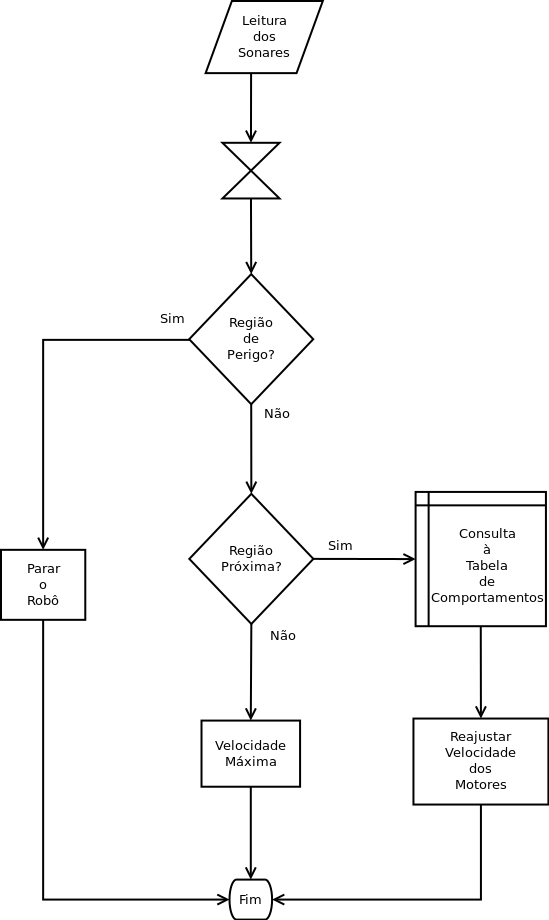
\includegraphics[width=0.8 \linewidth]{../../Imagens/ObstAvoid.png}
    \caption{Fluxograma da Rotina de Desvio de Obstáculos}
    \label{ObstAvoid}
  \end{figure}
 \pagebreak

 \section{Tabela Verdade}
\begin{table}[!htb]
\centering
\caption{}
\label{IA}
\begin{tabular}{|ccccc|c|}
\hline
{\color[HTML]{00009B} \textbf{$USS_0$}} & {\color[HTML]{00009B} \textbf{$USS_1$}} & {\color[HTML]{00009B} \textbf{$USS_2$}} & 
{\color[HTML]{00009B} \textbf{$USS_3$}} & {\color[HTML]{00009B} \textbf{$USS_4$}} & {\color[HTML]{FE0000} \textbf{Ação}} \\ 
\hline
{\color[HTML]{00009B} 0}                                     & {\color[HTML]{00009B} 0}                                    & {\color[HTML]{00009B} 0} 
 
                                  & {\color[HTML]{00009B} 0}                                    & {\color[HTML]{00009B} 1}                            
 
       & {\color[HTML]{FE0000} $E_L$}                                     \\ \hline
{\color[HTML]{00009B} 0}                                     & {\color[HTML]{00009B} 0}                                    & {\color[HTML]{00009B} 0} 
 
                                  & {\color[HTML]{00009B} 1}                                    & {\color[HTML]{00009B} 0}                            
 
       & {\color[HTML]{FE0000} $E_M$}                                     \\ \hline
{\color[HTML]{00009B} 0}                                     & {\color[HTML]{00009B} 0}                                    & {\color[HTML]{00009B} 0} 
 
                                  & {\color[HTML]{00009B} 1}                                    & {\color[HTML]{00009B} 1}                            
 
       & {\color[HTML]{FE0000} $E_M$}                                     \\ \hline
{\color[HTML]{00009B} 0}                                     & {\color[HTML]{00009B} 0}                                    & {\color[HTML]{00009B} 1} 
 
                                  & {\color[HTML]{00009B} 0}                                    & {\color[HTML]{00009B} 0}                            
 
       & {\color[HTML]{FE0000} $E_F$}                                     \\ \hline
{\color[HTML]{00009B} 0}                                     & {\color[HTML]{00009B} 0}                                    & {\color[HTML]{00009B} 1} 
 
                                  & {\color[HTML]{00009B} 0}                                    & {\color[HTML]{00009B} 1}                            
 
       & {\color[HTML]{FE0000} $E_F$}                                     \\ \hline
{\color[HTML]{00009B} 0}                                   & {\color[HTML]{00009B} 0}                                    & {\color[HTML]{00009B} 1}   
 
                                & {\color[HTML]{00009B} 1}                                    & {\color[HTML]{00009B} 0}                              
 
     & {\color[HTML]{FE0000} $E_F$}                                     \\ \hline
{\color[HTML]{00009B} 0}                                    & {\color[HTML]{00009B} 0}                                  & {\color[HTML]{00009B} 1}    
 
                               & {\color[HTML]{00009B} 1}                                    & {\color[HTML]{00009B} 1}                               
 
    & {\color[HTML]{FE0000} $E_F$}                                     \\ \hline
{\color[HTML]{00009B} 0}                                     & {\color[HTML]{00009B} 1}                                    & {\color[HTML]{00009B} 0} 
 
                                & {\color[HTML]{00009B} 0}                                    & {\color[HTML]{00009B} 0}                              
 
     & {\color[HTML]{FE0000} $D_M$}                                     \\ \hline
{\color[HTML]{00009B} 0}                                    & {\color[HTML]{00009B} 1}                                    & {\color[HTML]{00009B} 0}  
 
                                 & {\color[HTML]{00009B} 0}                                 & {\color[HTML]{00009B} 1}                                
 
   & {\color[HTML]{FE0000} $D_M$}                                     \\ \hline
{\color[HTML]{00009B} 0}                                    & {\color[HTML]{00009B} 1}                                    & {\color[HTML]{00009B} 0}  
 
                                 & {\color[HTML]{00009B} 1}                                    & {\color[HTML]{00009B} 0}                             
 
      & {\color[HTML]{FE0000} $E_F$}                                     \\ \hline
{\color[HTML]{00009B} 0}                                    & {\color[HTML]{00009B} 1}                                    & {\color[HTML]{00009B} 0}  
 
                                 & {\color[HTML]{00009B} 1}                                    & {\color[HTML]{00009B} 1}                             
 
      & {\color[HTML]{FE0000} $E_M$}                                  \\ \hline
{\color[HTML]{00009B} 0}                                     & {\color[HTML]{00009B} 1}                                    & {\color[HTML]{00009B} 1} 
 
                                  & {\color[HTML]{00009B} 0}                                    & {\color[HTML]{00009B} 0}                            
 
       & {\color[HTML]{FE0000} $D_F$}                                     \\ \hline
{\color[HTML]{00009B} 0}                                     & {\color[HTML]{00009B} 1}                                    & {\color[HTML]{00009B} 1} 
 
                                  & {\color[HTML]{00009B} 0}                                    & {\color[HTML]{00009B} 1}                            
 
       & {\color[HTML]{FE0000} $E_F$}                                     \\ \hline
{\color[HTML]{00009B} 0}                                     & {\color[HTML]{00009B} 1}                                    & {\color[HTML]{00009B} 1} 
 
                                  & {\color[HTML]{00009B} 1}                                    & {\color[HTML]{00009B} 0}                            
 
       & {\color[HTML]{FE0000} $E_F$}                                     \\ \hline
{\color[HTML]{00009B} 0}                                     & {\color[HTML]{00009B} 1}                                    & {\color[HTML]{00009B} 1} 
 
                                  & {\color[HTML]{00009B} 1}                                    & {\color[HTML]{00009B} 1}                            
 
       & {\color[HTML]{FE0000} $E_F$}                                     \\ \hline
{\color[HTML]{00009B} 1}                                     & {\color[HTML]{00009B} 0}                                    & {\color[HTML]{00009B} 0} 
 
                                  & {\color[HTML]{00009B} 0}                                    & {\color[HTML]{00009B} 0}                            
 
       & {\color[HTML]{FE0000} $D_L$}                                     \\ \hline
{\color[HTML]{00009B} 1}                                     & {\color[HTML]{00009B} 0}                                    & {\color[HTML]{00009B} 0} 
 
                                  & {\color[HTML]{00009B} 0}                                    & {\color[HTML]{00009B} 1}                            
 
       & {\color[HTML]{FE0000} Frente}                                     \\ \hline
{\color[HTML]{00009B} 1}                                     & {\color[HTML]{00009B} 0}                                    & {\color[HTML]{00009B} 0} 
 
                                  & {\color[HTML]{00009B} 1}                                    & {\color[HTML]{00009B} 0}                            
 
       & {\color[HTML]{FE0000} $E_M$}                                     \\ \hline
{\color[HTML]{00009B} 1}                                     & {\color[HTML]{00009B} 0}                                    & {\color[HTML]{00009B} 0} 
 
                                  & {\color[HTML]{00009B} 1}                                    & {\color[HTML]{00009B} 1}                            
 
       & {\color[HTML]{FE0000} $E_M$}                                     \\ \hline
{\color[HTML]{00009B} 1}                                     & {\color[HTML]{00009B} 0}                                    & {\color[HTML]{00009B} 1} 
 
                                  & {\color[HTML]{00009B} 0}                                    & {\color[HTML]{00009B} 0}                            
 
       & {\color[HTML]{FE0000} $D_F$}                                     \\ \hline
{\color[HTML]{00009B} 1}                                     & {\color[HTML]{00009B} 0}                                    & {\color[HTML]{00009B} 1} 
 
                                  & {\color[HTML]{00009B} 0}                                    & {\color[HTML]{00009B} 1}                            
 
       & {\color[HTML]{FE0000} $E_F$}                                     \\ \hline
{\color[HTML]{00009B} 1}                                     & {\color[HTML]{00009B} 0}                                    & {\color[HTML]{00009B} 1} 
 
                                  & {\color[HTML]{00009B} 1}                                    & {\color[HTML]{00009B} 0}                            
 
       & {\color[HTML]{FE0000} $E_F$}                                     \\ \hline
{\color[HTML]{00009B} 1}                                     & {\color[HTML]{00009B} 0}                                    & {\color[HTML]{00009B} 1} 
 
                                  & {\color[HTML]{00009B} 1}                                    & {\color[HTML]{00009B} 1}                            
 
       & {\color[HTML]{FE0000} $E_F$}                                     \\ \hline
{\color[HTML]{00009B} 1}                                     & {\color[HTML]{00009B} 1}                                    & {\color[HTML]{00009B} 0} 
 
                                  & {\color[HTML]{00009B} 0}                                    & {\color[HTML]{00009B} 0}                            
 
       & {\color[HTML]{FE0000} $D_M$}                                     \\ \hline
{\color[HTML]{00009B} 1}                                     & {\color[HTML]{00009B} 1}                                    & {\color[HTML]{00009B} 0} 
 
                                  & {\color[HTML]{00009B} 0}                                    & {\color[HTML]{00009B} 1}                            
 
       & {\color[HTML]{FE0000} $D_M$}                                     \\ \hline
{\color[HTML]{00009B} 1}                                     & {\color[HTML]{00009B} 1}                                    & {\color[HTML]{00009B} 0} 
 
                                  & {\color[HTML]{00009B} 1}                                    & {\color[HTML]{00009B} 0}                            
 
       & {\color[HTML]{FE0000} $D_M$}                                     \\ \hline
{\color[HTML]{00009B} 1}                                     & {\color[HTML]{00009B} 1}                                    & {\color[HTML]{00009B} 0} 
 
                                  & {\color[HTML]{00009B} 1}                                    & {\color[HTML]{00009B} 1}                            
 
       & {\color[HTML]{FE0000} Frente}                                     \\ \hline
{\color[HTML]{00009B} 1}                                     & {\color[HTML]{00009B} 1}                                    & {\color[HTML]{00009B} 1} 
 
                                  & {\color[HTML]{00009B} 0}                                    & {\color[HTML]{00009B} 0}                            
 
       & {\color[HTML]{FE0000} $D_F$}                                     \\ \hline
{\color[HTML]{00009B} 1}                                     & {\color[HTML]{00009B} 1}                                    & {\color[HTML]{00009B} 1} 
 
                                  & {\color[HTML]{00009B} 0}                                    & {\color[HTML]{00009B} 1}                            
 
       & {\color[HTML]{FE0000} $D_F$}                                     \\ \hline
{\color[HTML]{00009B} 1}                                     & {\color[HTML]{00009B} 1}                                    & {\color[HTML]{00009B} 1} 
 
                                  & {\color[HTML]{00009B} 1}                                    & {\color[HTML]{00009B} 0}                            
 
       & {\color[HTML]{FE0000} $D_F$}                                     \\ \hline
{\color[HTML]{00009B} 1}                                     & {\color[HTML]{00009B} 1}                                    & {\color[HTML]{00009B} 1} 
 
                                  & {\color[HTML]{00009B} 1}                                    & {\color[HTML]{00009B} 1}                            
 
       & {\color[HTML]{FE0000} $E_F$}                                    \\ \hline

\end{tabular}
\end{table}



\section{Sistemas de Tempo Real}
São sistemas computacionais que dependem não somente da correção dos dados computados, mas que sejam obtidos dentro de um intervalo 
de tempo 
pré determinado, que pode ser maior ou menor de acordo com a aplicação.
Na literatura, este período em que se espera que a resposta do sistema se dê é denominado \textit{deadline}.
Sistemas de tempo real podem ser classificados em dois tipos: \textit{soft} ou \textit{hard}.

Sistemas \textit{soft} são menos restritivos, tolerando eventuais perdas de \textit{deadline}; 
ao contrário dos sistemas \textit{hard}, em que estas perdas não são aceitáveis.  

Algumas características típicas, apesar de não obrigatórias, de sistemas de tempo real são limitações com relação ao tamanho, propósito específico e 
baixo custo \cite{silberschatz}.

\section{CRC}
Método de detecção de erros aleatórios, isto é, de dados corrompidos ao longo do processo de transmissão ou armazenamento da informação por exemplo 
por ruídos, mas não por um agente \textquoteleft inteligente\textquoteright{} externo que modifique os dados transmitidos, tal qual um 
\textit{malware} \cite{stigge}.

Consiste essencialmente em uma divisão polinomial \cite{stigge}, logo, pode ser implementado em \textit{hardware}, utilizando-se apenas registradores 
de deslocamento com conexões realimentadas \cite{peterson}, assim como em \textit{software}. 
Em suma, trata-se de acrescentar à mensagem digital original um sufixo, que tem seu valor definido por operações realizadas em função da mensagem 
binária que se intenta enviar e de um polinômio gerador.
Para o \textit{transceiver} nRF24L01+, dois polinômios geradores são utilizados: Eq. \ref{CRC_1} quando o dado cíclico adicionado é de 1 
\textit{byte} , e Eq. \ref{CRC_2}, para 2 \textit{bytes} \cite{nRF}.

Para uma descrição completa de como é implementado este método, vide \cite{stigge,peterson}.

\begin{equation}
\label{CRC_1}
G(X) = X^8 + X^2 + X + 1 
\end{equation}

\begin{equation}
\label{CRC_2}
G(X) = X^{16} + X^{12} + X^5 + 1 
\end{equation}

\section{PWM}
A modulação por largura de pulso é uma técnica de modulação que consiste em amostrar e codificar o sinal correspondente à mensagem na largura de um 
trem de pulsos de amplitude fixa, i.e. cada amostra da mensagem é convertida em um pulso retangular cuja duração expressa a amplitude do sinal 
modulante.

Um modulador PWM pode ser implementado utilizando-se um circuito comparador não inversor cuja entrada inversora liga-se à saída de um gerador de 
ondas tipo dente de serra (\textit{trailing edge modulation}), dente de serra invertida (\textit{leading edge modulation}  ou triangular 
(\textit{modulation on both edges}) e na entrada não inversora, o sinal modulante. 
Desta forma, quando a tensão da mensagem excede a amplitude da onda gerada, observa-se um sinal alto na saída, caso contrário, baixo, conforme 
ilustra a Fig. \ref{pwm_modulation_types}.

  \begin{figure}[H] %% TODO fonte: https://en.wikipedia.org/wiki/File:Three_PWM_types.svg
    \centering
    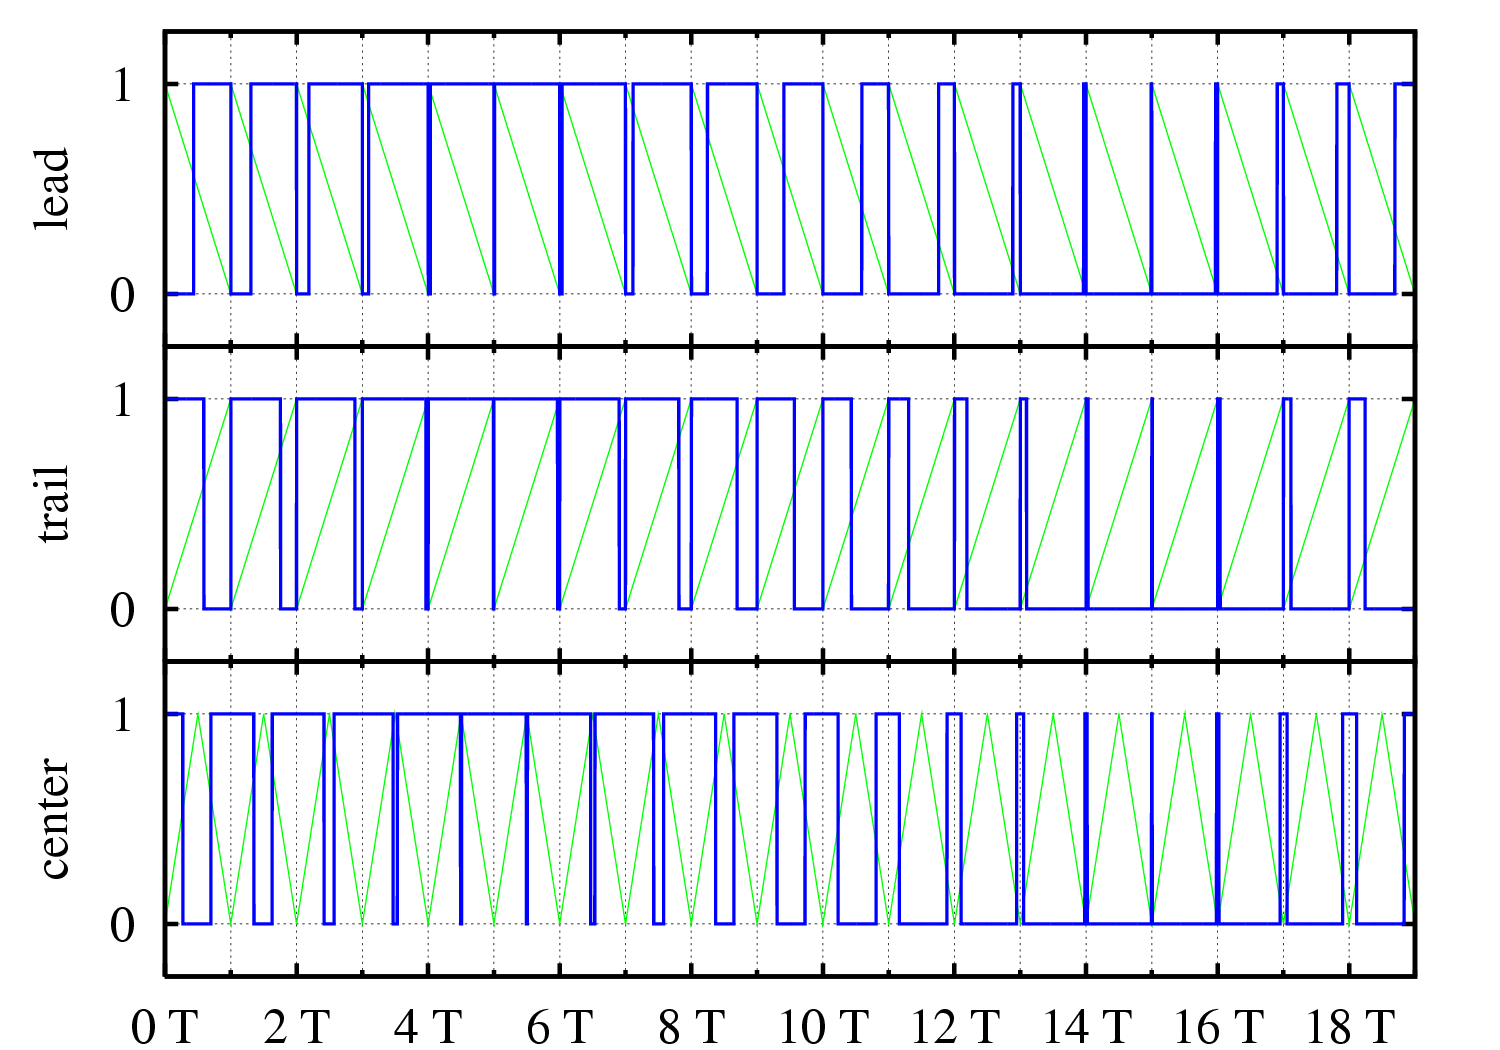
\includegraphics[width=0.7\linewidth]{../../Imagens/PWM_modulation_types.png}
    \caption{Três tipos de modulação PWM: \textit{trailing edge}, \textit{leading edge} e  \textit{both edges}, de cima pra baixo, respectivamente.}
    \label{pwm_modulation_types}
  \end{figure}
  
para uma descrição detalhada do circuito e simulações vide \cite{pwm_modulator}
  
  %TODO circuito corretor de erros:
%    First, the error amplifier accommodates feedback of the output PWM waveform in order to correct for any errors in the
% output voltage introduced by the comparator. Second, it adds a dc offset to the input voltage so that negative input voltages can be accommodated 
% by 
% the circuit.
%  
%  Because the supply voltage of the comparator directly impacts the output voltage, PWM circuits without feedback have no power supply rejection. In 
% this TI Design, the error amplifier acts as an inverting amplifier to the input signal, shown as a dc-coupled source VIN. By including the 
% comparator 
% inside the feedback loop of the error amplifier, and adding integration capacitor C1, the error amplifier now directly controls the average output 
% voltage
% 
% 


% ----------------------------------------------------------
% Anexos
% ----------------------------------------------------------
%% USPSC-Anexos.tex
% ---
% Inicia os anexos
% ---
\begin{anexosenv}

% Imprime uma página indicando o início dos anexos
\partanexos

% ---
\chapter{Exemplo de anexo}
% ---
Elemento opcional, que consiste em um texto ou documento não elaborado pelo autor, que serve de fundamentação, comprovação e ilustração, conforme a ABNT NBR 14724. \cite{nbr14724}.

O \textbf{ANEXO B} exemplifica como incluir um anexo em pdf.

\chapter{Acentuação (modo texto - \LaTeX)}
\begin{figure}[H]
	\begin{center}
	\caption{\label{fig_anexob}Acentuação (modo texto - \LaTeX)}
	\includegraphics[scale=1.0]{USPSC-AcentuacaoLaTeX.png} \\
	Fonte: \citeonline{comandos}
	\end{center}	
\end{figure}

\chapter{Símbolos úteis em \LaTeX}
\begin{figure}[H]
	\begin{center}
		\caption{\label{fig_anexoc}Símbolos úteis em \LaTeX}
		\includegraphics[scale=1.0]{USPSC-SimbolosUteis.png} \\
		Fonte: \citeonline{comandos}
	\end{center}	
\end{figure}


\chapter{Letras gregas em \LaTeX}
\begin{figure}[H]
	\begin{center}
		\caption{\label{fig_anexod}Letras gregas em \LaTeX}
		\includegraphics[scale=1.0]{USPSC-LetrasGregas.png} \\
		Fonte: \citeonline{comandos}
	\end{center}	
\end{figure}

\end{anexosenv}


%---------------------------------------------------------------------
% INDICE REMISSIVO
%--------------------------------------------------------------------
%% USPSC-IndicexRemissivos.tex
% ---
% Inicia os Índices Remissivos
% ---
%---------------------------------------------------------------------
% INDICE REMISSIVO
%--------------------------------------------------------------------
\phantompart
\printindex
%---------------------------------------------------------------------


%---------------------------------------------------------------------

\end{document}
